\chapter[Experimentos]{Experimentos}
\label{chapter_experimentos}

Neste capítulo são apresentados os experimentos realizados durante a pesquisa. Esses experimentos visam avaliar o desempenho de diversas abordagens bio-inspiradas (algoritmos evolutivos e baseados em colônias de formigas), incluindo o algoritmo proposto nesta dissertação (MACO/NDS), quando empregadas na resolução de dois problemas discretos com muitos objetivos. 

Para facilitar a análise dos resultados, esses experimentos foram divididos em 4 etapas distintas de acordo com os objetivos desejados. Na primeira etapa, cinco algoritmos evolutivos multiobjetivos (AEMOs), encontrados da literatura, foram avaliados em problemas discretos de 2 a 6 objetivos. O objetivo dessa etapa é analisar o comportamento desses algoritmos de acordo com o número de objetivos tratados. Na segunda etapa, a fim de se desenvolver a base para a elaboração do algoritmo MACO/NDS pra o PRM multiobjetivo, avaliaram-se diversas estratégias para a construção de uma solução em um ACO mono-objetivo. A terceira etapa de experimentos contou com o algoritmo proposto (MACO/NDS) em sua versão final, ou seja, com a melhores estratégias observadas na segunda etapa de experimentos. O objetivo da terceira etapa foi avaliar o MACO/NDS contra os algoritmos \textit{many-objective} vistos até então (NSGA-III, MOEA/D, AEMMT e AEMMD) nos dois problemas (PMM e PRM) em instâncias com formulações a partir de 4 objetivos. A última etapa de experimentos conta com a adição de mais três métodos em relação a etapa anterior: o SPEA2-SDE, o MOEA/D-ACO e o MOACS. O objetivo dessa última seção é avaliar o comportamento dos algoritmos em instâncias mais complexas dos problemas da mochila e do roteamento. Além disso, na quarta etapa, é utilizada a métrica hiper-volume na avaliação dos resultados.

\section{Ambiente de teste}

Esta seção descreve a metodologia empregada nos experimentos, isto é, os algoritmos utilizados, as formas de avaliação e a apresentação dos resultados. Os seguintes algoritmos multiobjetivos foram utilizados em nossos experimentos:

\acresetall
\begin{itemize}
	\item \ac{NSGA-II} \cite{Deb2002};
	\item \ac{NSGA-III} \cite{Deb2014};
	\item \ac{SPEA2} \cite{Zitzler2002};
	\item \ac{SPEA2-SDE} \cite{Spea2SDE};
	\item \ac{MOEA/D} \cite{Zhang2007};
	\item \ac{MEAMT}. Nesta dissertação, referenciamos esse trabalho pelo nome proposto originalmente em português, \ac{AEMMT} \cite{Brasil2013};
	\item \ac{MEANDS}. Nesta dissertação, referenciamos esse trabalho pelo nome proposto originalmente em português, \ac{AEMMD} \cite{Lafeta2017};
	\item \ac{MOEA/D-ACO} \cite{Ke2013};
	\item \ac{MOACS} \cite{Riveros2016}
	\item e o ACO proposto: \ac{MACO/NDS}.
\end{itemize}

Todos esses algoritmos foram avaliados considerando dois problemas discretos multiobjetivos: o \ac{PMM} e o Problema \ac{PRM}. A fim  de verificar o comportamento dos algoritmos em relação ao número de objetivos, diversas formulações foram consideradas, avaliando-se problemas desde dois até seis objetivos. Assim como o número de funções objetivo, a topologia da rede (PRM) e a quantidade de itens (PMM) também afetam a complexidade. Portanto, elaboraram-se instâncias diferentes para cada problema. No PRM, são consideradas seis redes de diferentes complexidades, as quais também foram utilizadas em \cite{LafetaThesis}. No PMM variou-se a quantidade de itens em 30, 40, 50, 100 e 200.

Parte das métricas utilizadas para avaliar os algoritmos são paramétricas, ou seja, dependem do conhecimento prévio sobre a fronteira de Pareto do problema. Como foi inviável a obtenção do conjunto Pareto ótimo exato para cada instância, antes de executar os experimentos, foi calculado um conjunto aproximado para cada um dos cenários de teste. Tal conjunto aproximado, denominado ``Pareto aproximado'' ou ``fronteira de Pareto aproximada'', foi obtido através de várias execuções de todos os algoritmos utilizados nos experimentos sobre o cenário. Além disso, no caso das instâncias de redes do PRM, esses resultados foram comparados com os Paretos aproximados obtidos em \cite{Lafeta2017}.

Considerando as quatro etapas de experimentos, foram usadas 4 métricas multiobjetivo para se avaliar o desempenho dos algoritmos, além do tempo de execução. São elas:

\begin{itemize}
	\item \textbf{\ac{ER}}: sendo $S$ o conjunto de soluções encontrado pelo algoritmo e $P$ a fronteira de Pareto aproximada. A taxa de erro é a porcentagem das soluções de $S$ que não aparecem em P, como mostra a fórmula a seguir:
	\begin{equation}
		ER = \frac{\sum\limits_{s \in S} e(s)}{|S|}, \quad
		e(s) = 
		\begin{cases} 
			0 & s \in P \\
			1 & s \notin P
		\end{cases}
	\end{equation}
	Por exemplo, tome $S=\{A, B, C, D, F\}$ e $P=\{A,D\}$. Como 3 das soluções de $S$ não estão em $P$, a taxa de erro é $3/5=0,6$, ou seja, 60\%.
	\item \textbf{\ac{GD}}: mede a distância das soluções no conjunto encontrado pelo algoritmo ($S$) para as soluções mais próximas na fronteira de Pareto aproximada ($P$). A distância euclidiana ($dist$) de cada $s \in S$ é medida em relação a cada $p \in P$. A menor distância para $p$ de cada $s$ é então elevada ao quadrado e adicionada à soma. Ao final, retorna-se o valor da raiz quadrada do somatório dividido pela quantidade de elementos em $S$. O cálculo da $GD$ é dada por:
	\begin{equation}GD = \frac{\sqrt{\sum\limits_{s \in S} \min\limits_{p \in P} dist(s, p)^2}}{|S|}\end{equation}
	Por exemplo, considere um problema bi-dimensional, onde o $S$ encontrado é $\{(1,2), (5,2), (3,7)\}$ e o Pareto aproximado $P$ vale $\{(2,3), (5,2)\}$. O primeiro passo é encontrar as menores distâncias de cada elemento de $S$ para $P$. Tomando o primeiro elemento de $S$, $s_1=(1,2)$, calcula-se as distâncias para $p_1$ e $p_2$. $dist(s_1, p_1)=\sqrt{(1-2)^2 + (2-3)^2}=\sqrt{2}$ e $dist(s_1, p_2)=\sqrt{(1-5)^2 + (2-2)^2}=4$. Portanto, a menor distância de $s_1$ para $P$ é $\sqrt{2}$. O mesmo cálculo é feito para $s_2$ e $s_3$, onde obtém-se que a menor distância de $s_2$ para $P$ é 0 e a menor distância de $s_3$ para $P$ é $\sqrt{17}$. Logo, a distância $GD$ é dada por $\frac{\sqrt{\sqrt{2} + 0 + \sqrt{17}}}{3}=0,78$.
	\item \textbf{\ac{GDp}}: similar à definição anterior, mas ao invés de considerar todas as soluções no cálculo de distância, considera apenas aquelas que não fazem parte do Pareto aproximado, ou seja, elimina do cálculo as distâncias que valem 0. No exemplo dado para o $GD$, o valor de $GDp$ seria dado por $\frac{\sqrt{\sqrt{2} + \sqrt{17}}}{2}=1,18$.
	\item \textbf{\ac{PS}}: número absoluto de soluções encontradas ($S$) que fazem parte do Pareto aproximado ($P$), o qual é obtido por:
	\begin{equation}
		PS = \sum\limits_{s \in S} a(s), \quad
		a(s) = 
		\begin{cases} 
			1 & s \in P \\
			0 & s \notin P
		\end{cases}
	\end{equation}
	Por exemplo, dado $S=\{A, B, C, D, F\}$ e $P=\{A,D\}$. Como 2 das soluções de $S$ estão em $P$, o valor do $PS$ é 2.
	\item \textbf{\ac{HV}}: métrica multiobjetivo que independe do conhecimento prévio da fronteira de Pareto. Mede o volume da figura geométrica $m$-dimensional (sendo $m$ o número de objetivos) formada pelas soluções encontradas considerando a origem do sistema de coordenadas como um ponto arbitrário $p_{ref}$, chamado de ponto de referência. As coordenadas de $p_{ref}$ são diferentes para cada cenário (problema, formulação de objetivos e instância) e são determinadas pelo pior valor encontrado em cada um dos objetivos considerando a união das soluções dos Paretos obtidos em cada execução. Se o PMM de 5 objetivos e 100 itens é executado 10 vezes, por exemplo, extraem-se os 10 resultados e colocam-se as soluções em um único conjunto $S_{todos}$. Varre-se $S_{todos}$ procurando pelo pior valor em cada uma das 5 coordenadas e cria-se uma solução fictícia para os valores encontrados. Essa solução fictícia é então utilizada como ponto de referência ($p_{ref}$) para o PMM de 5 objetivos e 100 itens. Em nossos experimentos, foi utilizada a implementação do cálculo de hiper-volume descrito em \citeonline{Bradstreet2012}.
	Por exemplo, considere um problema de minimização bi-dimensional e tome $S=\{(6,3), (9,2), (4,5), (5,4), (3,6)\}$ como o conjunto de soluções encontradas. O ponto de referência será dado pelo ponto formado pelo pior valor obtido na primeira coordenada e pelo pior valor obtido na segunda, ou seja, $p_{ref}=(9,6)$. A \autoref{fig_hipervolume} mostra a representação gráfica de $S$ e $p_{ref}$. Neste exemplo, o valor do hiper-volume é dado pelo volume da forma geométrica destacada em cinza ($F$), ou seja, $hv=13$. Dessa forma, é fácil visualizar que quanto mais representativo e distribuído o conjunto de soluções, maior o volume da forma geométrica, ou seja, o hiper-volume deve ser maximizado.
	\begin{figure*}[!htbp]
		\centering
		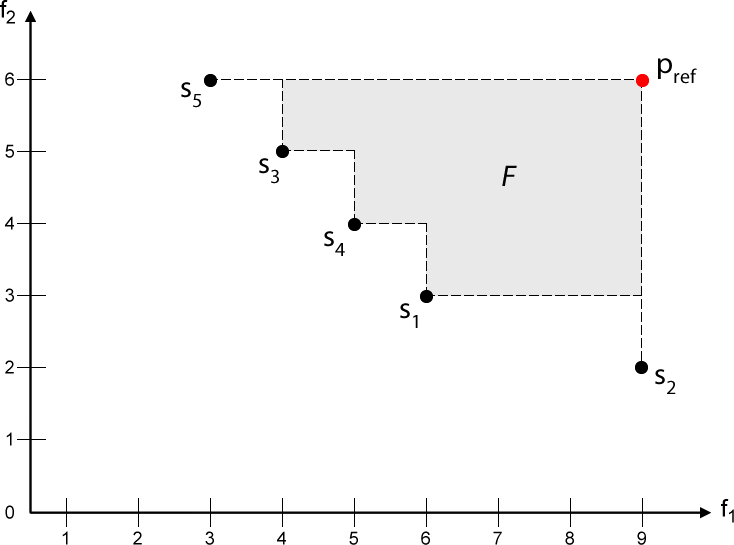
\includegraphics[width=0.8\textwidth]{cap_experimentos/figs/hipervolume}
		\caption{\label{fig_hipervolume}Exemplo de hiper-volume}
	\end{figure*}
	\item Tempo: tempo médio, em segundos, necessário para a execução do algoritmo. Foi aferido a partir das diferenças de tempo entre o momento em que o algoritmo inicia a execução até o momento quando retorna o conjunto de soluções encontradas. O valor final do tempo é obtido através da média entre três execuções.
\end{itemize}

Para obter os valores dessas métricas, nas seções \ref{section_experimentos_etapa1} e \ref{section_experimentos_etapa3}, foram feitas 100 execuções de cada algoritmo em cada cenário. Na Seção \ref{section_experimentos_etapa4}, que utiliza o hiper-volume, o número de execuções foi 30. O número reduzido de execuções na última etapa se deve à maior dificuldade em se calcular o hiper-volume em relação às demais métricas. Uma ressalva também é feita quanto ao tempo de execução, que foi calculado a partir da média aritmética de três execuções isoladas de cada algoritmo em cada cenário. O número reduzido de experimentos para se obter os valores de tempo se deve a dois fatores. Primeiramente, executar cada algoritmo isoladamente em uma máquina leva um tempo considerável, o que torna inviável a execução de vários experimentos. Além disso, o tempo não varia muito de uma execução para outra, fazendo com que a média entre três simulações seja suficiente. 

A apresentação dos resultados é feita de três formas: gráficos, tabelas e testes de hipótese. Os gráficos utilizam barras para mostrar os valores da média dos resultados de cada métrica considerando todas as execuções para o algoritmo e cenário indicados. Em alguns gráficos, os desvios padrões são representados por linhas verticais sobre as barras. Os mesmos valores mostrados de maneira gráfica também são disponibilizados na forma de tabelas no apêndice \ref{ape_tabelas_exp}. Além disso, em alguns dos experimentos, é utilizado o testes de hipótese teste Z (\textit{Z test}) para verificar se a superioridade de algum algoritmo em relação aos demais possui significância estatística. O teste de hipótese é apresentado através de uma tabela, onde cada linha representa um cenário e cada coluna uma métrica de desempenho, os sinais de ``$>$'' e ``$<$'' indicam se o método analisado obteve resultado significativamente maior ou menor em relação a seu adversário, enquanto o sinal ``$=$'' indica que não é possível determinar de forma significativa a superioridade entre eles. Além dos sinais, no teste de hipótese, as células são coloridas em verde, caso o algoritmo analisado tenha obtido melhor desempenho, em vermelho, caso o desempenho tenha sido pior e em branco, nos casos onde o desempenho foi similar.

\section{Análise Comparativa dos Algoritmos Evolutivos}
\label{section_experimentos_etapa1}

Os experimentos apresentados nesta seção serviram como base para a elaboração de um artigo publicado no \ac{BRACIS} \cite{Franca2017}. Na elaboração do artigo, o autor da presente dissertação implementou e efetuou os experimentos com o PMM, enquanto os experimentos com o PRM foram realizados por outro autor e também estudante de pós-graduação Thiago Fialho Lafetá, quem investigou o PRM em sua própria dissertação \cite{LafetaThesis}. Posteriormente, o PRM também foi implementado e o novo ambiente serviu de base para os experimentos descritos nas próximas seções. Os resultados no PRM gerados pelo Thiago Fialho são apresentados nessa seção, pois suas conclusões foram importantes na definição dos próximos passos da dissertação.

Nessa primeira etapa, foram realizados experimentos visando a análise comparativa dos AGs multiobjetivos NSGA-II, NSGA-III, SPEA2, MOEA/D e AEMMT nos problemas da mochila e do roteamento multicast. O número de objetivos varia entre dois e seis e, no PRM, três redes são testadas, enquanto o PMM lida com instâncias de 30, 50 e 100 itens. Além dos cinco algoritmos mencionados, avalia-se também uma pequena modificação no AEMMT chamada de AEMMT-F que remove o limite no tamanho do arquivo de soluções não-dominadas (\textit{free size}). As avaliações dos algoritmos são feitas com base em métricas relacionadas ao Pareto aproximado calculado e permitem um melhor entendimento sobre o comportamento dos algoritmos. Isso facilitou a identificação de pontos fortes e fracos de cada estratégia, ajudando na elaboração do MACO/NDS, que é o novo algoritmo proposto neste trabalho.

Durante os experimentos, os algoritmos NSGA-II, NSGA-III, SPEA2, MOEA/D e AEMMT foram avaliados em diferentes cenários dos dois problemas investigados (PRM e PMM). Ao todo, 30 cenários de teste foram considerados (15 para cada problema):

\begin{itemize}
	\item PMM: 5 formulações de objetivos (2 a 6) e 3 instâncias (30, 50 e 100 itens). Os valores de cada objetivo e dos pesos dos itens são gerados aleatoriamente para cada instância do problema, conforme descrito na Seção \ref{section_problemas_pmm}.
	\item PRM: 5 formulações de objetivos ($P_2$ a $P_6$) e 3 redes ($R_1$, $R_2$ e $R_3$). Tanto as formulações quanto as redes estão descritas na Seção \ref{section_problemas_prm}.
\end{itemize}

Para cada um dos cenários foi obtida um conjunto de Pareto aproximado, através de múltiplas execuções dos 5 algoritmos testados. A Tabela \ref{table_exp1_paretos} mostra a cardinalidade de cada Pareto encontrado.

\begin{table}[!htbp]
	\centering
	\caption{Conjunto de Pareto considerado para os cenários investigados na primeira etapa de experimentos}
	\label{table_exp1_paretos}
	\begin{tabular}{c|rrr|rrr}
		& \multicolumn{3}{c|}{\textbf{PRM}} & \multicolumn{3}{c}{\textbf{PMM}} \\ \hline
		Objetivos & R1         & R2       & R3        & 30 itens  & 50 itens & 100 itens \\ \hline
		2         & 14         & 9        & 6         & 15        & 67       & 170       \\
		3         & 30         & 18       & 17        & 106       & 501      & 6288      \\
		4         & 122        & 72       & 60        & 425       & 986      & 88374*    \\
		5         & 424        & 326      & 551       & 1765      & 5213     & 176868*   \\
		6         & 1196       & 657      & 1078      & 5800      & 35760*   & 248198*   \\ \hline
	\end{tabular}
\end{table}

Na Tabela \ref{table_exp1_paretos}, a quantidade de elementos nos paretos do PMM é demasiadamente grande para as formulações \textit{many-objective} com 100 itens. Isso acontece porque o espaço de busca do problema da mochila cresce exponencialmente com o número de itens. Esse crescimento é potencializado com o número de objetivos considerado, ou seja, quanto maior a quantidade de funções objetivos na formulação, maior o número de soluções que serão não-dominadas. O asterisco ao lado de alguns valores no PMM significa que não foi possível estabilizar o Pareto, ou seja, a cada rodada de execuções dos algoritmos, novas soluções eram encontradas. Tal comportamento motivou a realização dos experimentos da etapa 4 (Seção \ref{section_experimentos_etapa4}), nos quais não se usa um Pareto pré-definido para se avaliar os algoritmos. Apesar disso, os resultados para o problema de 100 itens ainda são relevantes, pois mesmo que os Paretos não sejam estáveis, comparam-se as execuções dos algoritmos contra o conjunto com todas as soluções encontradas, possibilitando determinar o algoritmo com melhor potencial para encontrar boas soluções nos diferentes cenários dos problemas multiobjetivos.

Os resultados utilizados no cálculo das métricas de desempenho $ER$, $GD$ e $PS$ foram obtidos a partir da média entre 100 execuções de cada algoritmo. Nessas execuções foram adotados os parâmetros de configuração listados na Tabela \ref{table_exp1_parametros}. Os parâmetros foram retirados de trabalhos anteriores \cite{LafetaThesis, Brasil2013, Ishibuchi2015}. Na tabela, o asterisco em ``número de gerações'' indica que nem todos os algoritmos seguem esse parâmetro. O AEMMT executa 9 mil gerações para o PRM e 7500 para o PMM. Isso acontece, pois esse algoritmo gera apenas 1 filho por ciclo no PRM e apenas 2 no PMM necessitando, portanto, de mais gerações para fazer o mesmo número de avaliações de novos indivíduos. No problema da mochila com 100 itens, devido à complexidade do problema, dobrou-se a quantidade de gerações. Ainda na tabela \ref{table_exp1_parametros}, o termo ``variável'' indica que a taxa de mutação adotada varia de acordo com a instância do problema. Nos experimentos realizados, foi empregada uma taxa de mutação de 6\% para o PMM de 30 itens, 4\% para o de 50 itens e 2\% para o de 100 itens, similar aos valores utilizados em \cite{Ishibuchi2015}. Esses valores foram empregados em todos os algoritmos.

\begin{table}[!htbp]
	\caption{Parâmetros utilizados pelos AEMOs na 1ª etapa, de acordo com o problema tratado.}
	\label{table_exp1_parametros}
	\begin{center}
		\begin{tabular}{c|r|r}
			\textbf{Parâmetro} & \textbf{(A) PRM} &  \textbf{(B) PMM} \\ %\hline
			\hline
			Tamanho da população                    &    90 &      150 \\ %\hline
			Número de gerações*                     &   100 (9000*) &      100 (7500*) \\ %\hline
			Taxa de crossover                       & 100\% &    100\% \\ %\hline
			Taxa de mutação                         &  20\% & variável \\ %\hline
			Tamanho da vizinhança (MOEA/D)          &    10 &       10 \\ %\hline
			Tamanho das tabelas (AEMMT)             &    30 &       50 \\ %\hline
			Tamanho da tabela de dominância (AEMMT) &    90 &      150 \\ %\hline
			Número de subdivisões (NSGA-III)        &     8 &        8 \\
			\hline
		\end{tabular}
	\end{center}
\end{table}

As Figuras \ref{fig_exp1_pmm_30}, \ref{fig_exp1_pmm_50} e \ref{fig_exp1_pmm_100} mostram, respectivamente, os resultados para o PMM de 30, 50 e 100 itens. Nas Figuras \ref{fig_exp1_prm_r1}, \ref{fig_exp1_prm_r2} e \ref{fig_exp1_prm_r3} são apresentados os resultados dos algoritmos para o PRM considerando as redes $R_1$, $R_2$ e $R_3$, respectivamente. Uma análise consolidada, considerando a média entre as três instâncias de cada problema, é apresenta nas Figuras \ref{fig_exp1_pmm_todos} (PMM) e \ref{fig_exp1_prm_todos} (PRM).

\begin{figure*}[!htbp]
	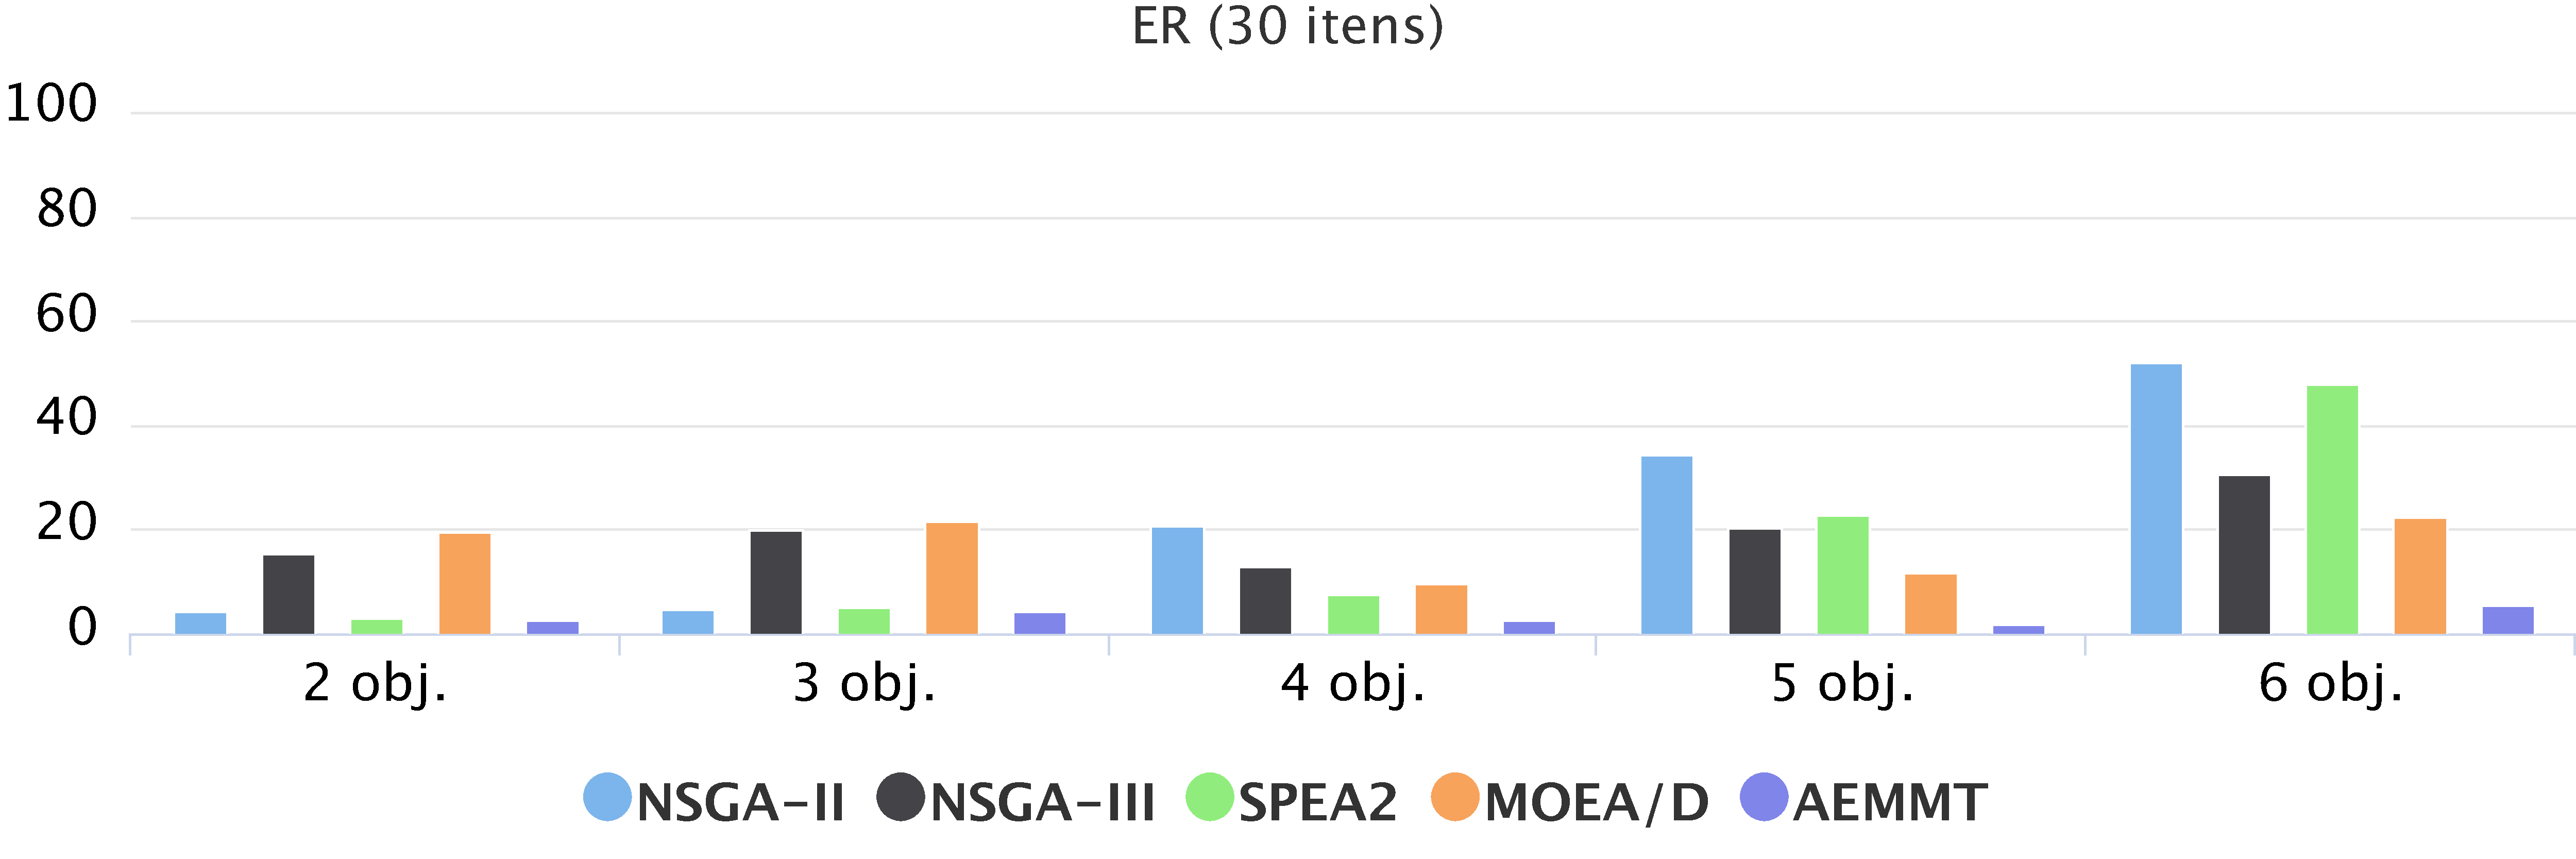
\includegraphics[width=1\textwidth]{cap_experimentos/figs/etapa1/er-mkp-30}
	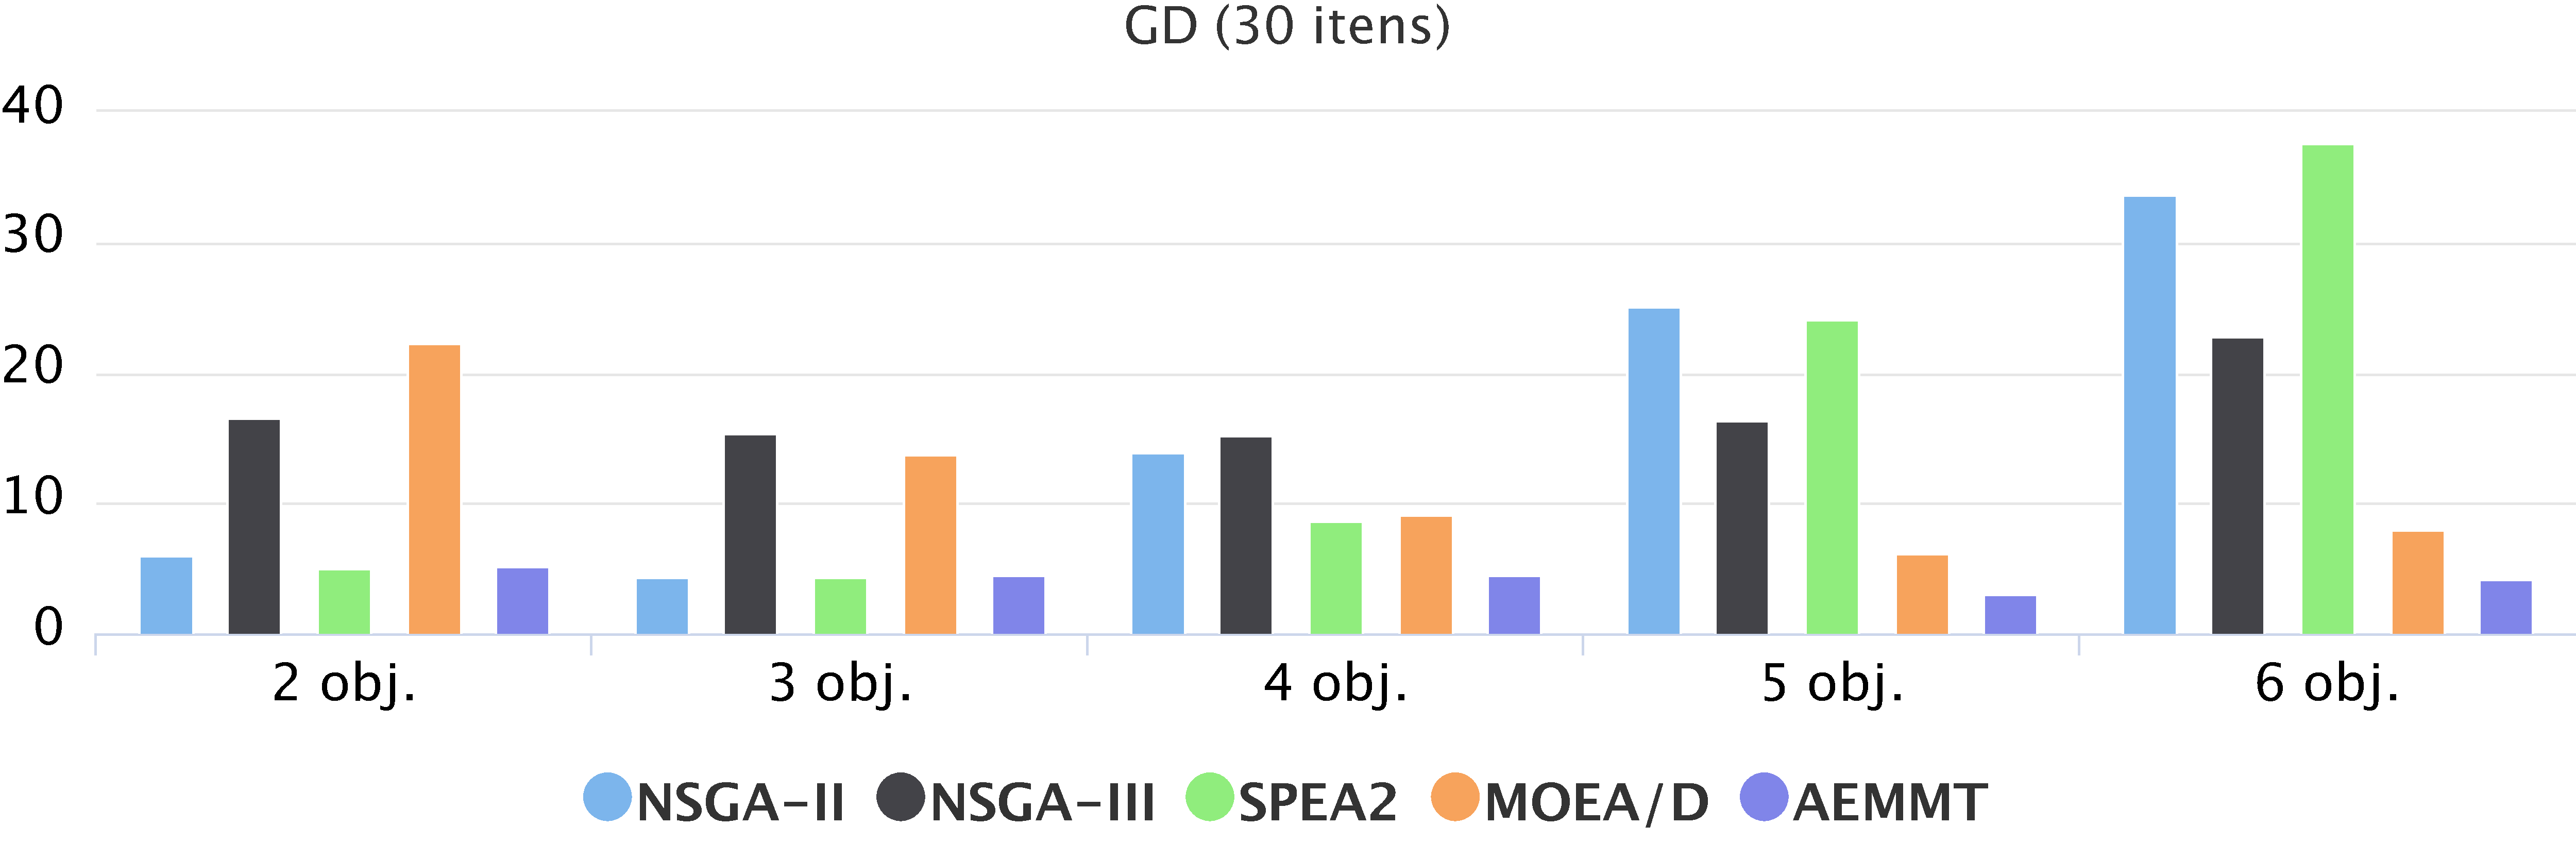
\includegraphics[width=1\textwidth]{cap_experimentos/figs/etapa1/gd-mkp-30}
	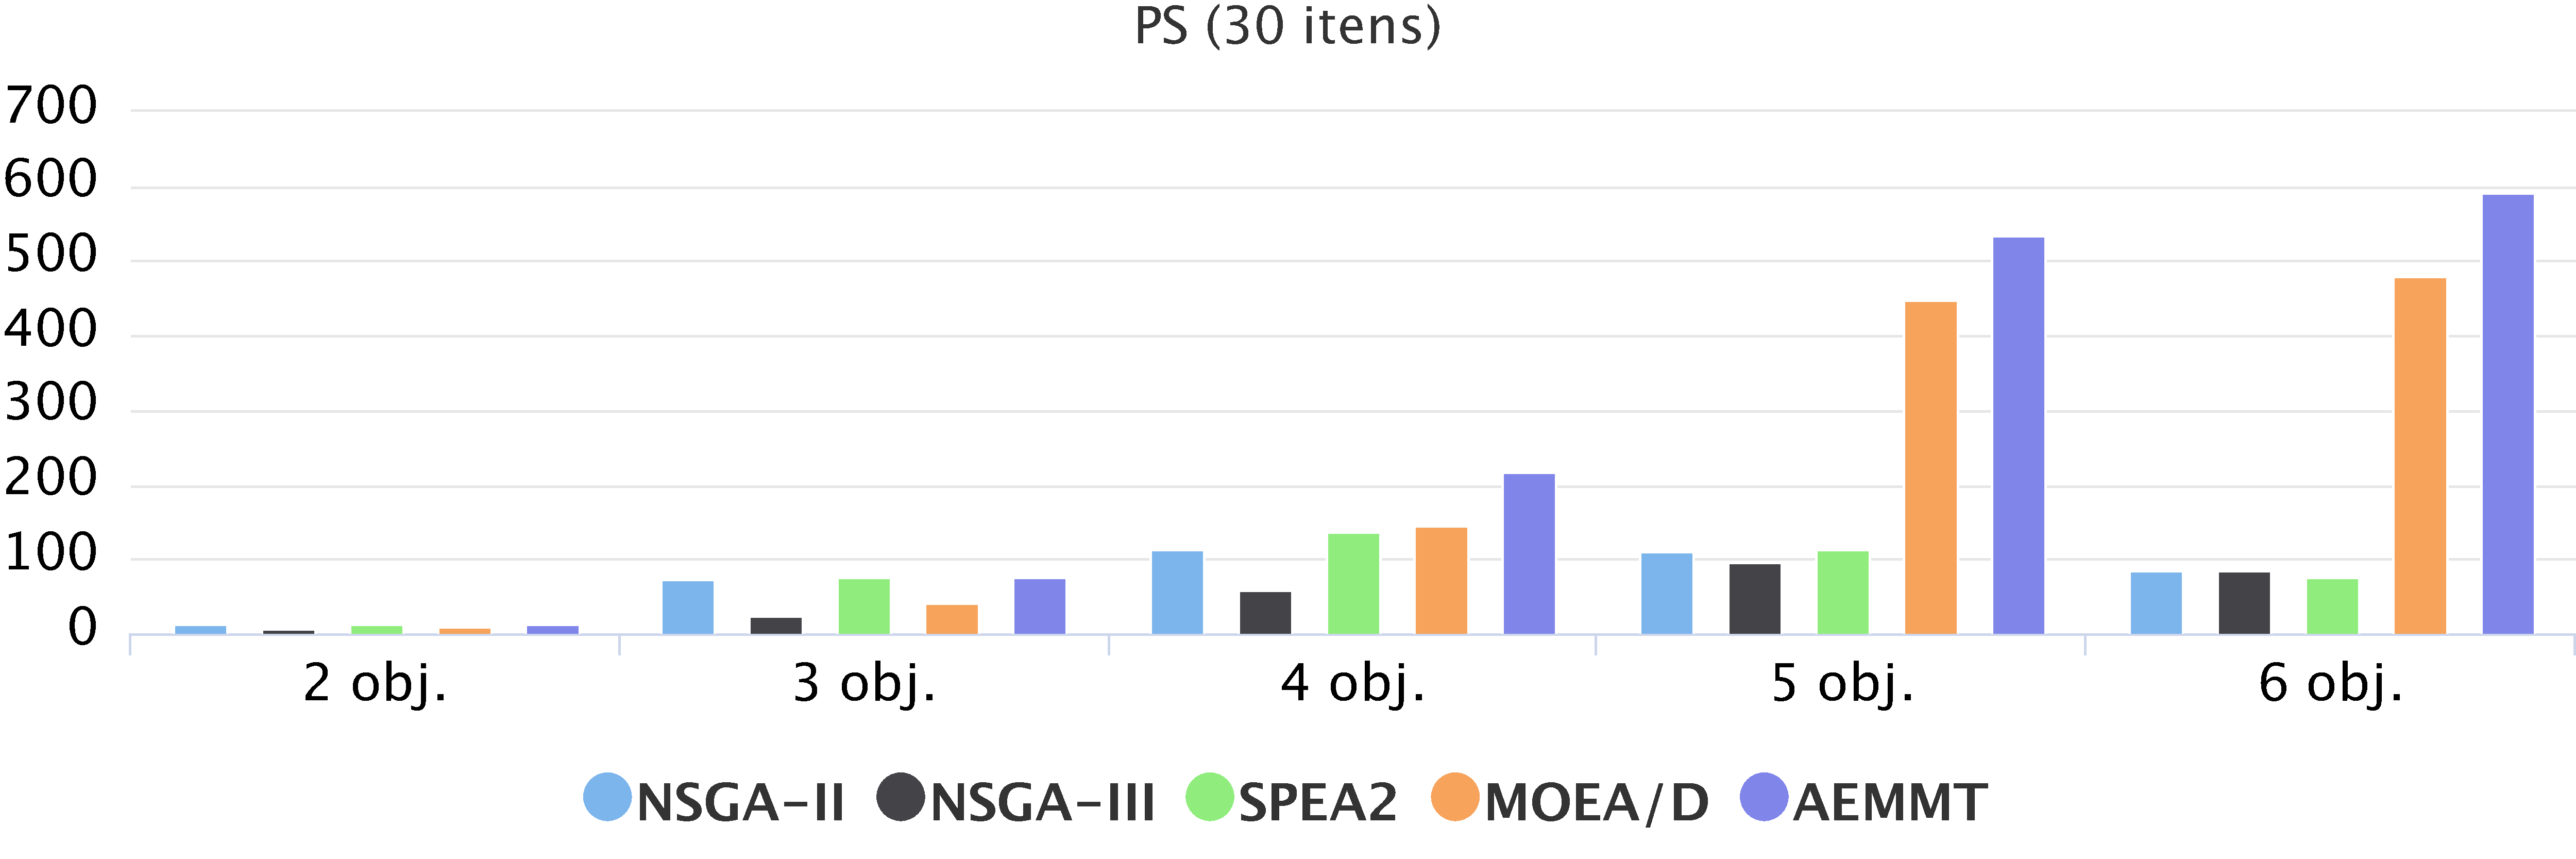
\includegraphics[width=1\textwidth]{cap_experimentos/figs/etapa1/ps-mkp-30}
	\caption{\label{fig_exp1_pmm_30}Desempenho dos algoritmos na 1ª etapa para o PMM com 30 itens}
\end{figure*}

Como pode ser observado na \autoref{fig_exp1_pmm_30}, o PMM com 30 itens é um problema relativamente simples e, no geral, os métodos de otimização multiobjetivo alcançam bons resultados. Até 4 objetivos, apenas o MOEA/D passou a marca de 20\% de erro. Para 2 e 3 objetivos, os algoritmos NSGA-II, SPEA2 e AEMMT apresentaram desempenhos muito similares, resultando nos melhores percentuais de erro entre todos os algoritmos avaliados. A partir de 4 objetivos é possível notar uma queda considerável no desempenho dos algoritmos multiobjetivos clássicos (NSGA-II e SPEA-2). Considerando-se todas as formulações de objetivo no PMM, os melhores resultados foram obtidos pelo AEMMT que manteve o erro abaixo de 6\% em todos os casos. Analisando a métrica $GD$, obtêm-se as mesmas conclusões tiradas a partir do $ER$. Isto é, considerando todas as formulações, o AEMMT gera os melhores resultados. Por outro lado, apesar de terem um desempenho muito bom nos problemas de 2 e 3 objetivos, os valores da métrica GD para o NSGA-II e o SPEA2 apresentam resultados ruins a partir de 4 objetivos. O tamanho da fronteira de Pareto encontrada, medida pelo $PS$, é maior nos algoritmos MOEA/D e AEMMT. Esse comportamento é esperado no MOEA/D, pois diferentemente dos demais AEMOs, ele não aplica uma limitação sobre o tamanho do arquivo que armazena as soluções não-dominadas. O alto valor de $PS$ também é esperado no AEMMT, pois, apesar da tabela de não-dominância ser limitada, o resultado final é dado pelas soluções não dominadas considerando todas as tabelas, ou seja, o limite sobre o tamanho do Pareto é mais fraco que os demais algoritmos. Considerando-se os valores das três métricas em todas as formulações de objetivos para o PMM de 30 itens, está claro que, no geral, o AEMMT é o melhor dentre os métodos testados.

\begin{figure*}[!htbp]
	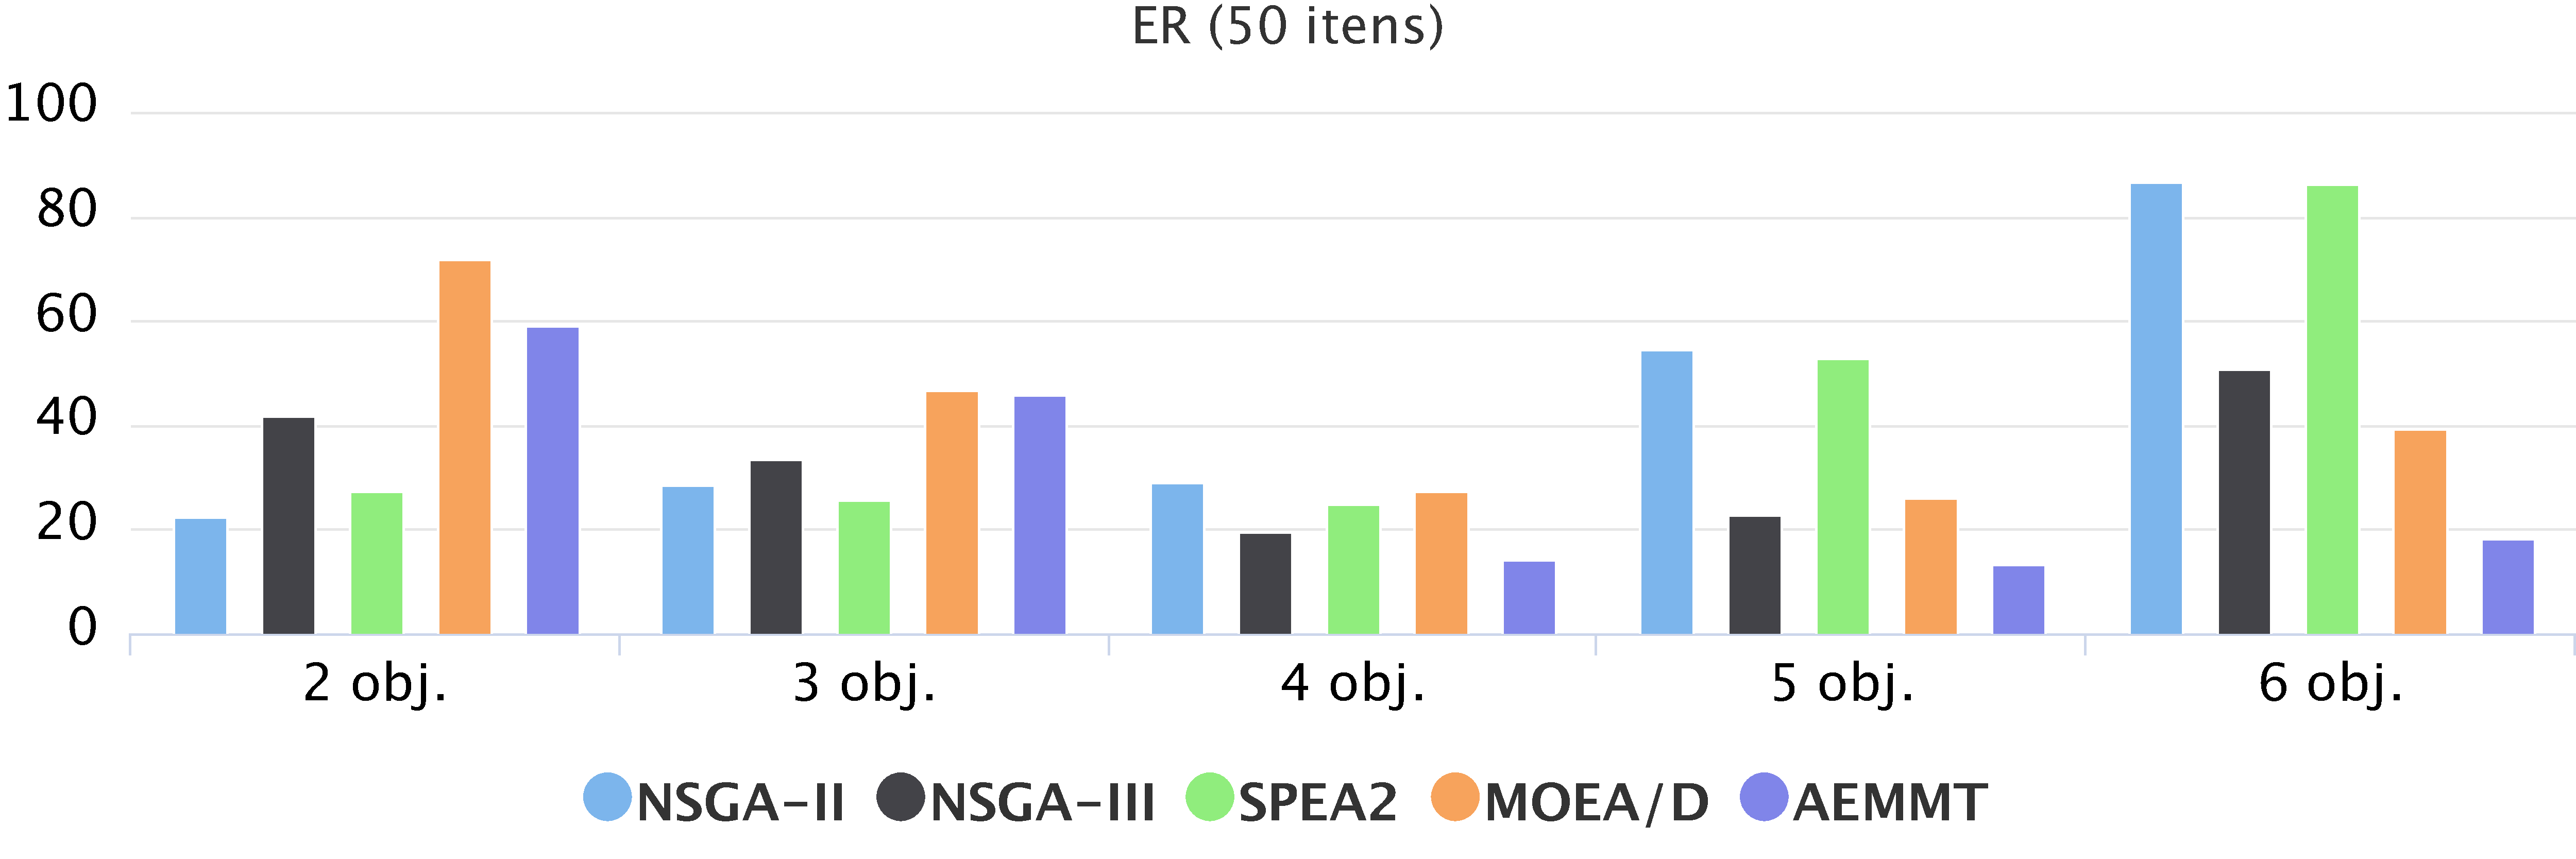
\includegraphics[width=1\textwidth]{cap_experimentos/figs/etapa1/er-mkp-50}
	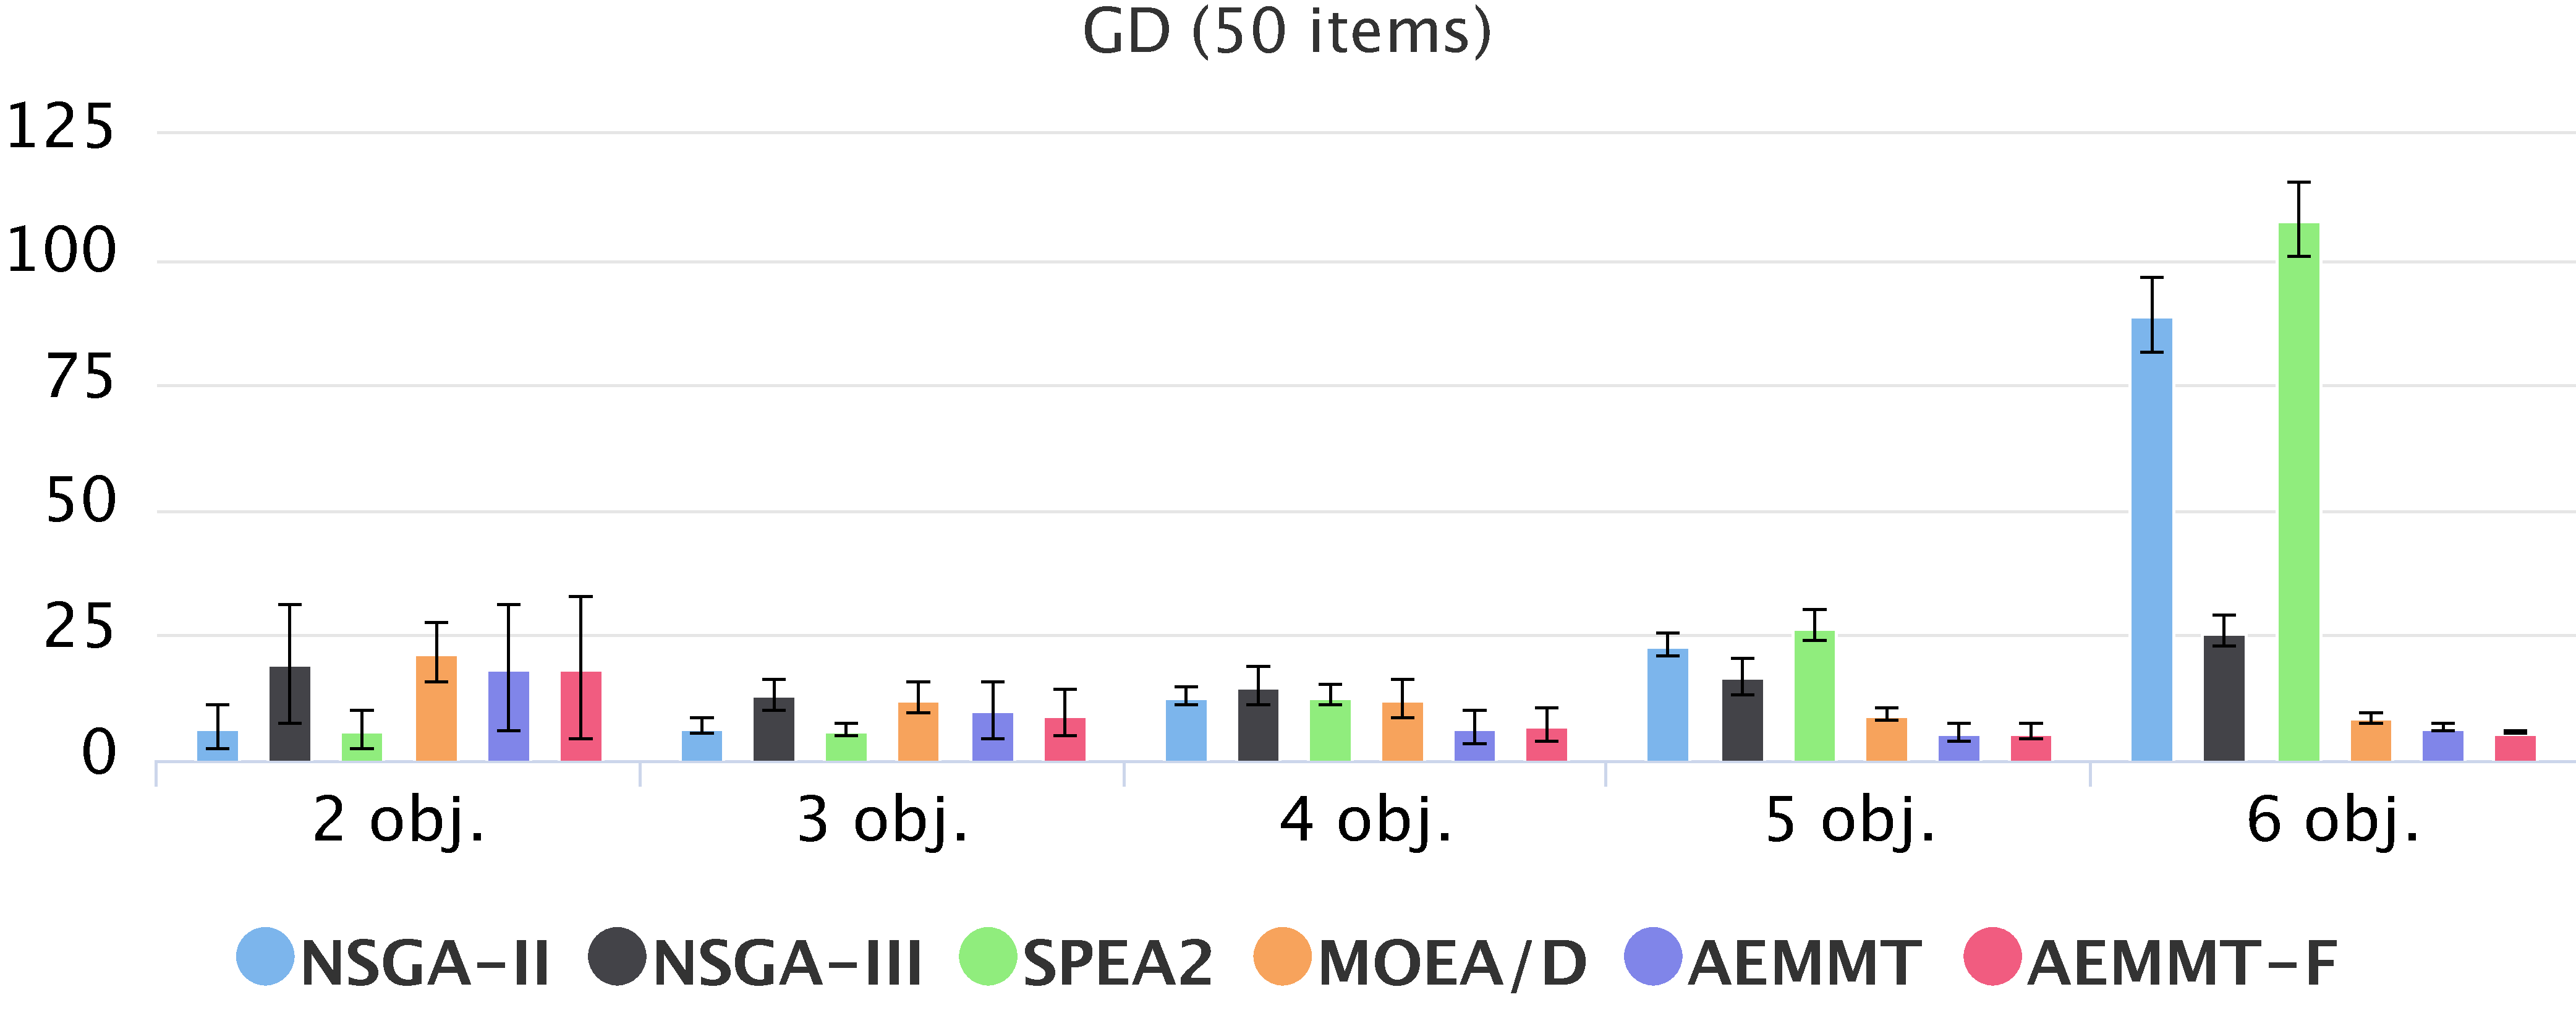
\includegraphics[width=1\textwidth]{cap_experimentos/figs/etapa1/gd-mkp-50}
	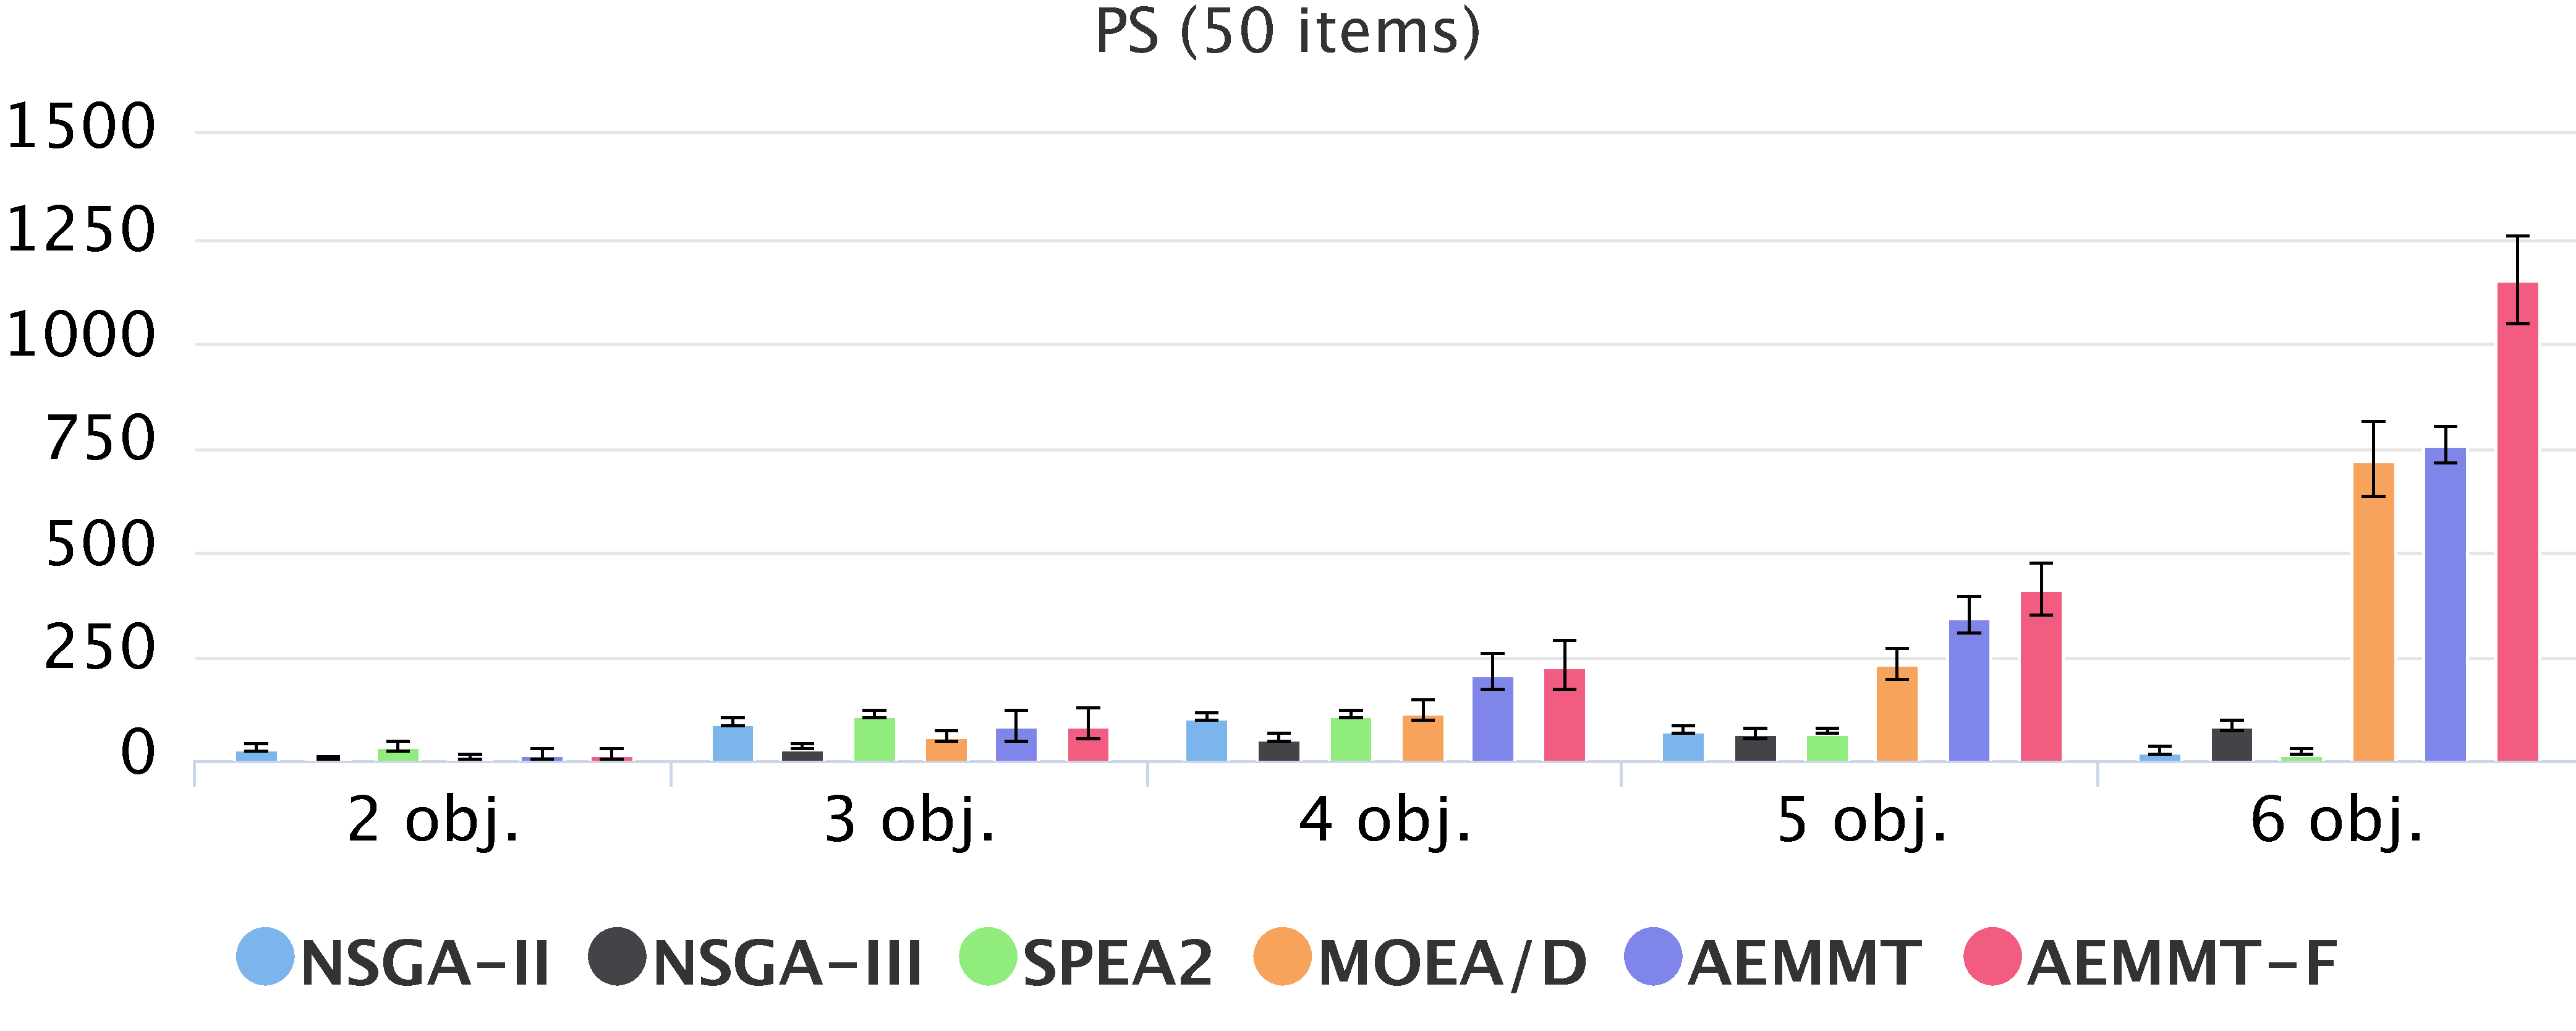
\includegraphics[width=1\textwidth]{cap_experimentos/figs/etapa1/ps-mkp-50}
	\caption{\label{fig_exp1_pmm_50}Desempenho dos algoritmos na 1ª etapa para o PMM com 50 itens}
\end{figure*}

O PMM com 50 itens (\autoref{fig_exp1_pmm_50}) é um problema mais complexo que sua versão com 30 itens e os algoritmos têm mais dificuldade para convergir para o Pareto aproximado, o que pode ser comprovado pelas taxas de erro maiores em relação ao experimento anterior. Nessa instância, é mais evidente  o comportamento de cada algoritmo em função das diferentes formulações de objetivos. Nas formulações com 2 e 3 objetivos, os algoritmos clássicos (NSGA-II e SPEA2) são imbatíveis, independentemente da métrica analisada. A partir de 4 objetivos, o AEMMT assume a primeira posição e é o melhor algoritmo tanto para $ER$ quanto para $GD$ e $PS$. Depois do AEMMT, para 4 objetivos, a menor taxa de erro é atingida pelo NSGA-III, seguido pelos SPEA2, MOEA/D e NSGA-II. Para 5 objetivos, o NSGA-III continua apresentando a segunda menor taxa de erro, enquanto o MOEA/D obtém resultado melhor que o SPEA2. Para seis objetivos, o MOEA/D tem $ER$ pior apenas que o AEMMT e o NSGA-III apresenta o terceiro melhor resultado. Com relação ao $GD$, o MOEA/D obtém o segundo melhor desempenho para as formulações \textit{many-objective} (a partir de 4 objetivos) e o NSGA-III obtém o terceiro melhor, excluindo a formulação com 4 objetivos, onde o SPEA2 é melhor. O $PS$, a partir de 4 objetivos, é dominado pelos algoritmos AEMMT e MOEA/D, o NSGA-III possui um comportamento mais parecido com os algoritmos clássicos que com os algoritmos \textit{many-objective}.  É possível notar que, com o aumento do número de objetivos, o NSGA-II e o SPEA2 pioram enquanto o AEMMT mantém o $ER$ e o $GD$ estáveis e melhora o $PS$. O MOEA/D é o segundo melhor algoritmo para problemas \textit{many-objectives} e o NSGA-III é o terceiro. Para o PMM de 50 itens, o AEMMT é a melhor opção para muitos objetivos, assim como observado no PMM com 30 itens.

\begin{figure*}[!htbp]
	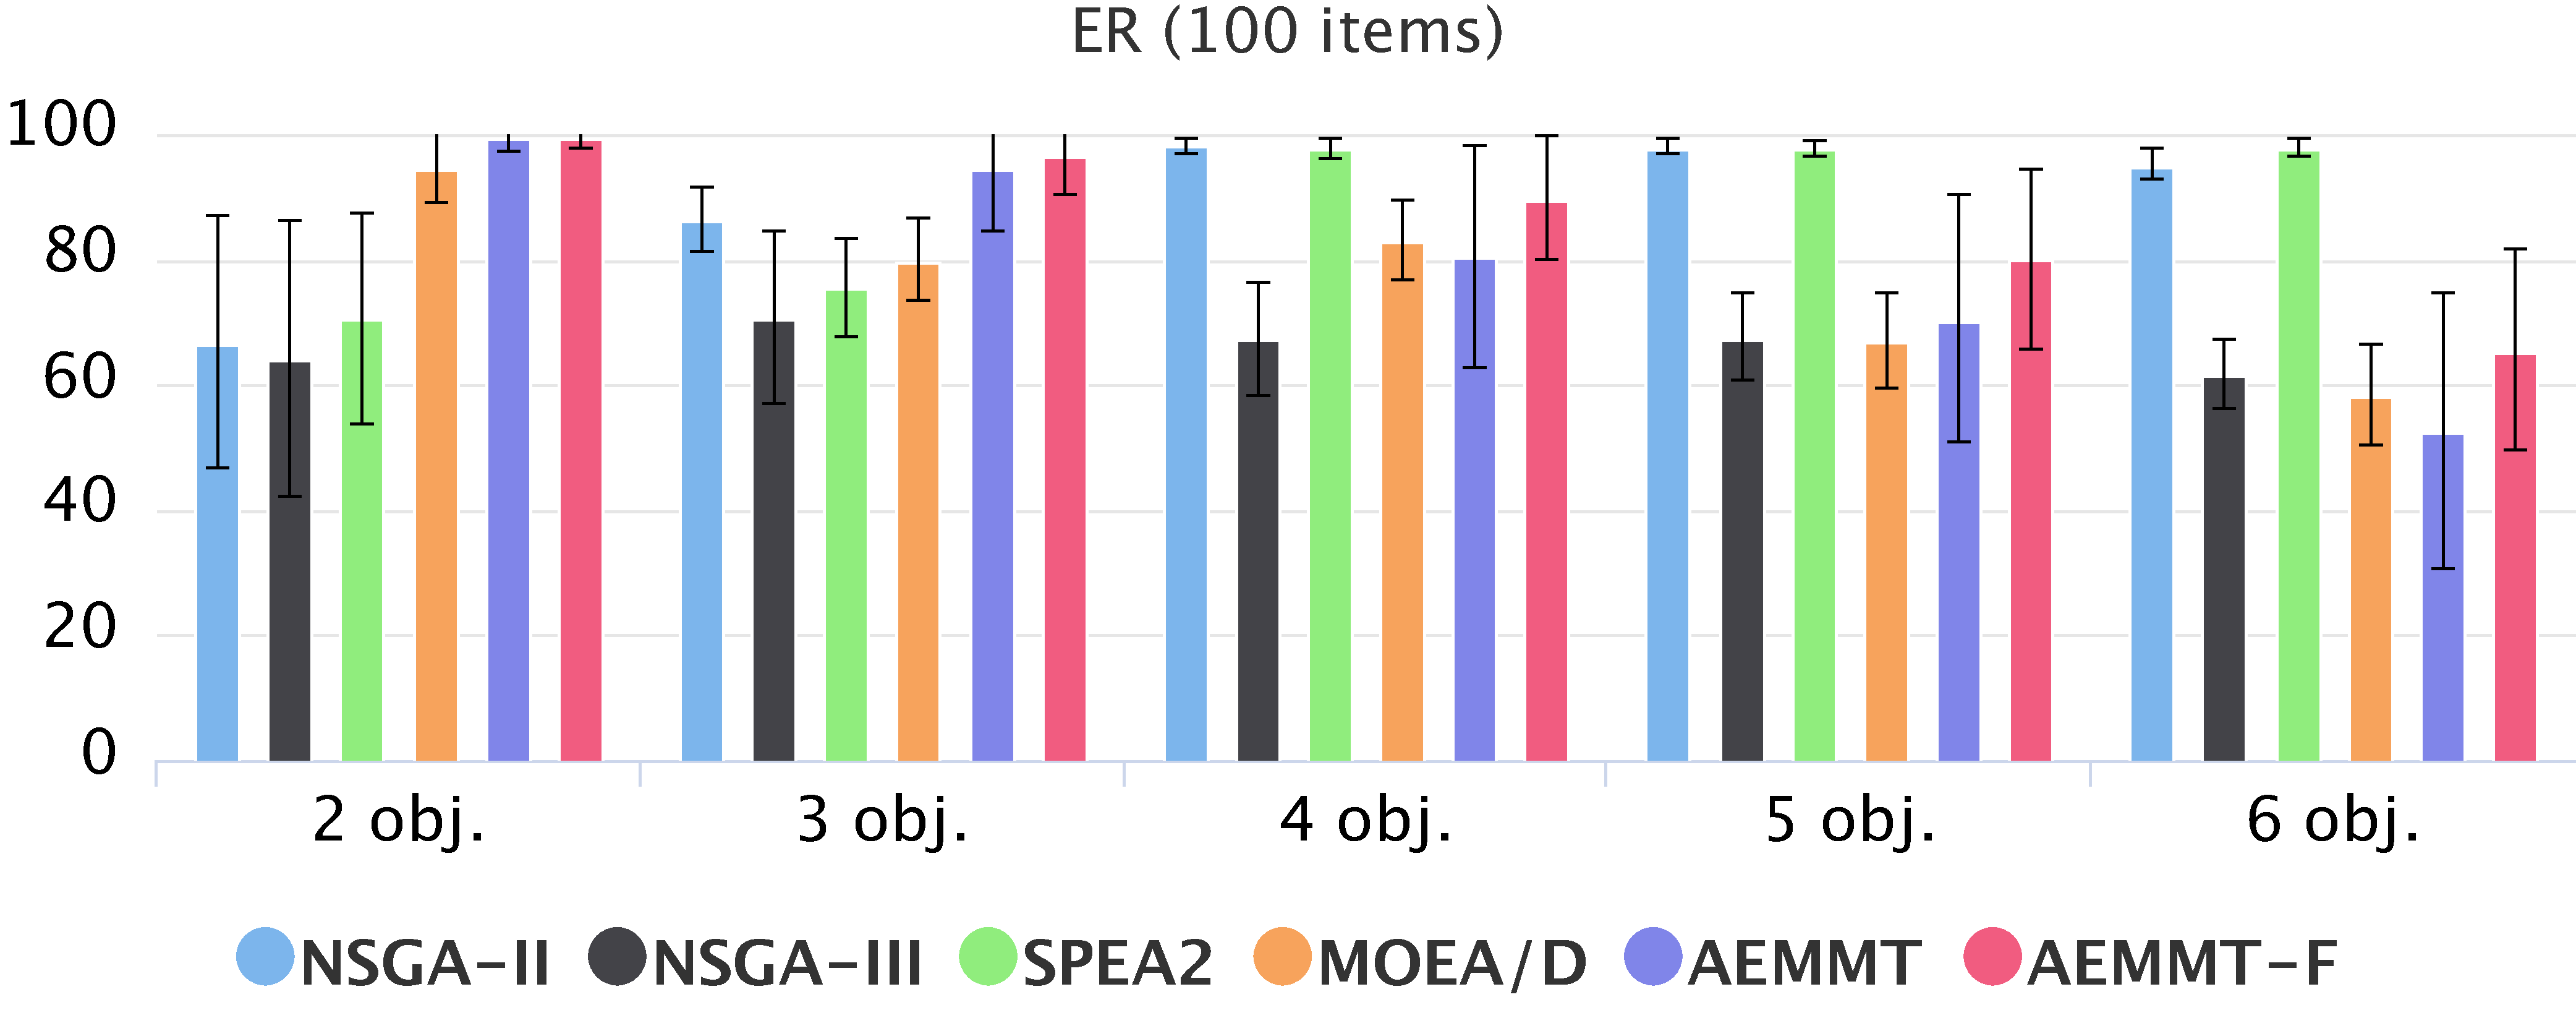
\includegraphics[width=1\textwidth]{cap_experimentos/figs/etapa1/er-mkp-100}
	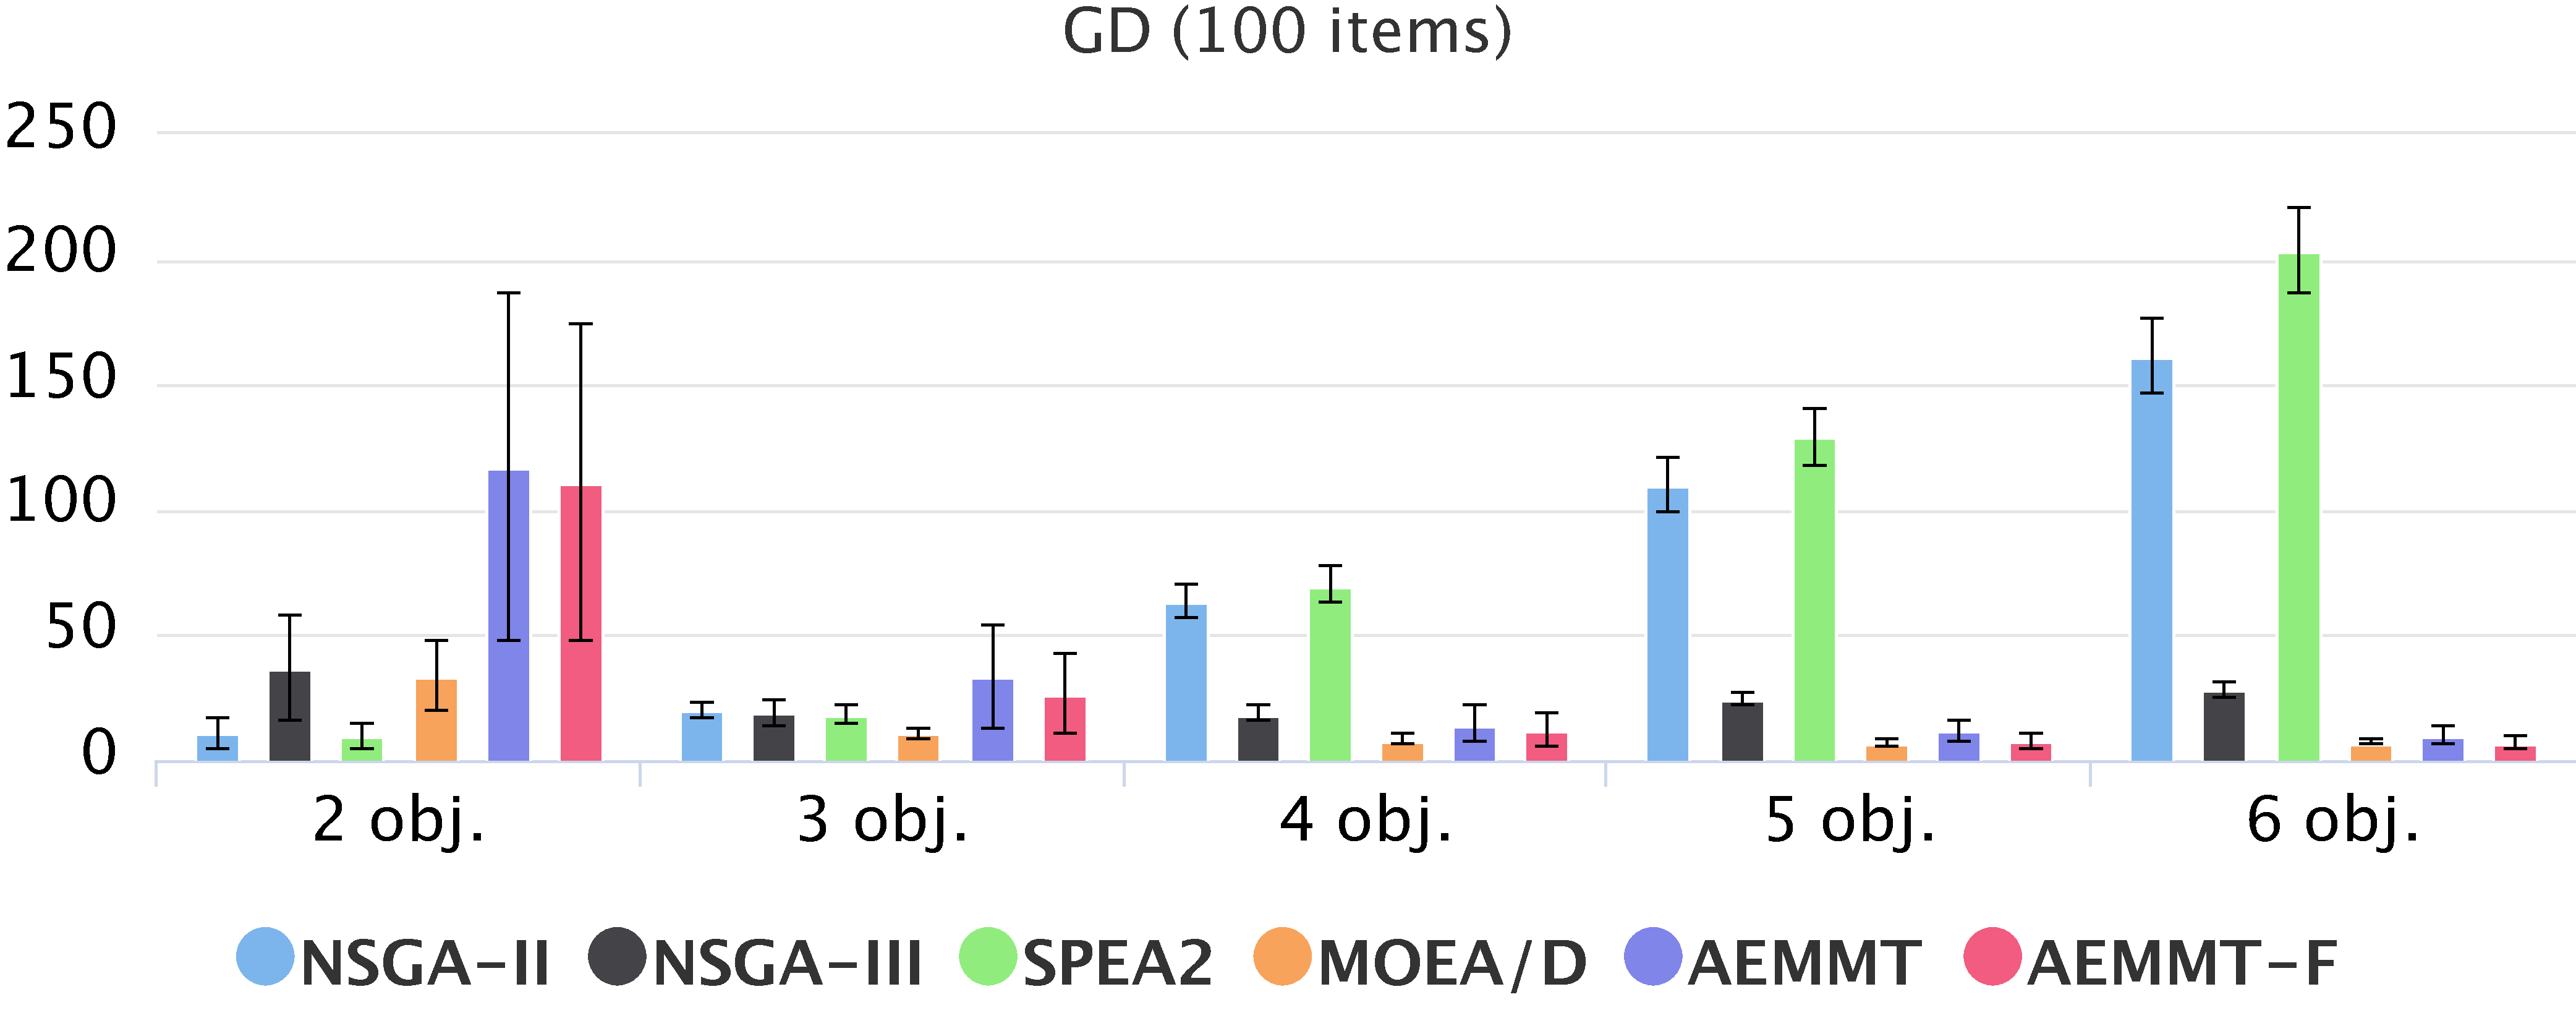
\includegraphics[width=1\textwidth]{cap_experimentos/figs/etapa1/gd-mkp-100}
	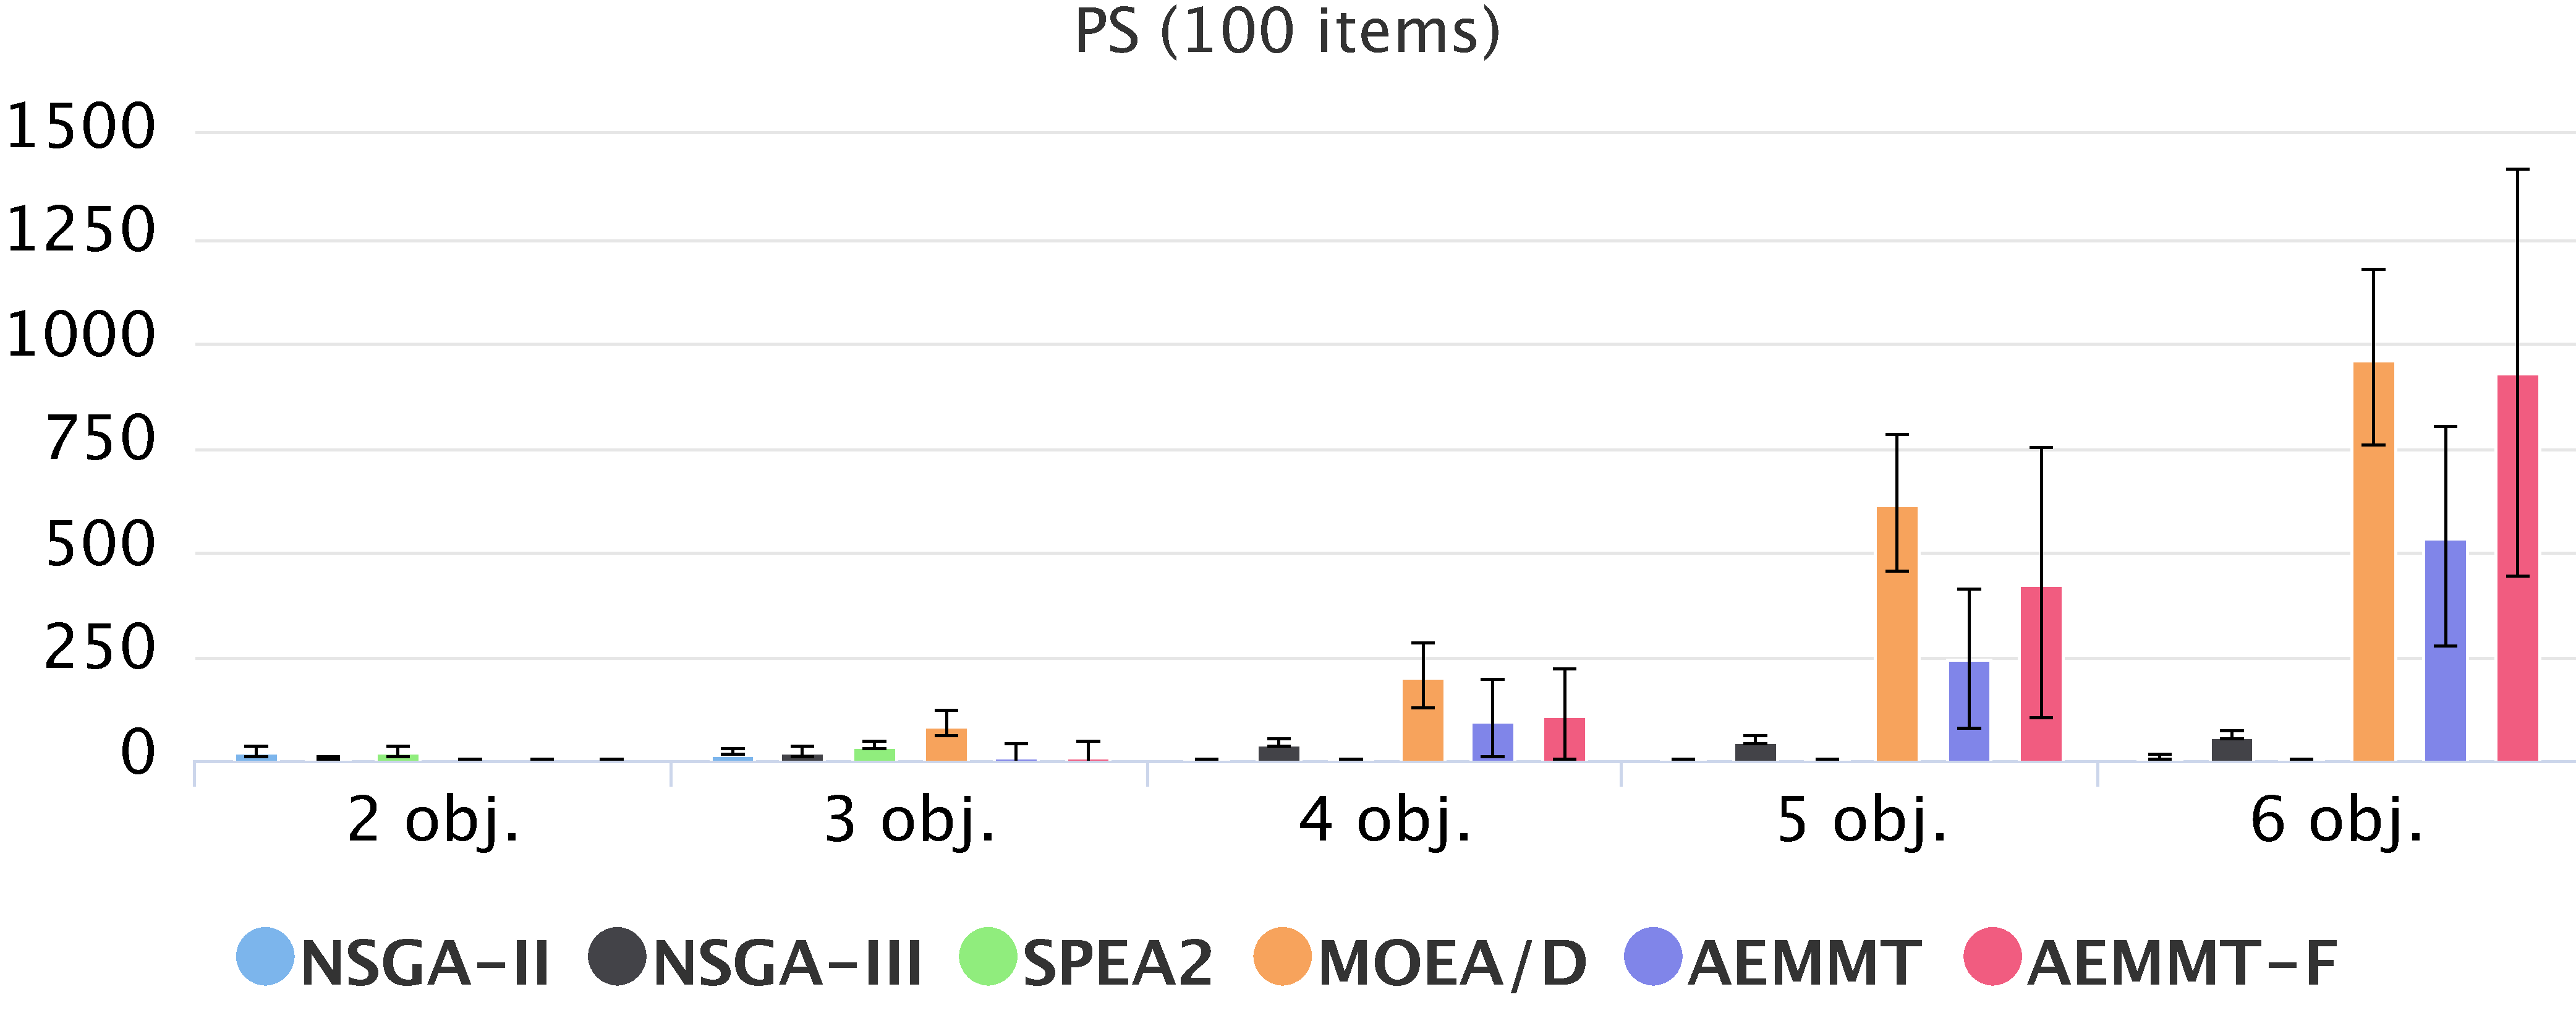
\includegraphics[width=1\textwidth]{cap_experimentos/figs/etapa1/ps-mkp-100}
	\caption{\label{fig_exp1_pmm_100}Desempenho dos algoritmos na 1ª etapa para o PMM com 100 itens}
\end{figure*}

O tamanho do espaço de busca no problema da mochila é $2^n$, sendo $n$ o número de itens. Portanto, a complexidade do PMM com 100 itens, cujos resultados são apresentados na \autoref{fig_exp1_pmm_100}, é muito maior que nas instâncias anteriores. Nesse caso, não foi possível encontrar um Pareto estável para as formulações de 4, 5 e 6 objetivos. Dessa forma, apesar das métricas $ER$, $GD$ e $PS$ serem um bom indicativo de desempenho entre os algoritmos, a melhor forma de avaliação seria o hiper-volume. Um experimento similar, mas utilizando o hiper-volume, é apresentado na Seção \ref{section_experimentos_etapa4}. É difícil avaliar o problema considerando 100 itens, pois, a partir dos resultados apresentados para a métrica de erro (ER) na \autoref{fig_exp1_pmm_100}, é possível perceber que poucos algoritmos conseguiram encontrar boas soluções. Considerando a métrica $ER$, o algoritmo com melhor desempenho retornou uma taxa de erro acima de 50\%. O NSGA-III apresentou o menor $ER$ nos cenários de 2, 3, 4 e 5 objetivos, enquanto que na formulação de 6, os melhores desempenhos nessa métrica foram obtidos pelos AEMMT e MOEA/D. Com relação ao $GD$, o NSGA-II e o SPEA2 apresentaram os melhores resultados para 2 objetivos. Na formulação de 3 objetivos em diante, o MOEA/D foi o algoritmo com menor $GD$, sendo que , a partir de 4 objetivos, o AEMMT obteve desempenho similar. A situação se repete ao analisar o $PS$. A partir de 3 objetivos, o MOEA/D traz um conjunto maior de soluções na fronteira de Pareto, seguido pelo AEMMT a partir de 4 objetivos. Em problemas com muitos objetivos, o AEMMT e o MOEA/D são as melhores opções, sendo que o AEMMT apresenta uma taxa de erro levemente menor e o MOEA/D obtém um valor de $PS$ consideravelmente melhor. Para problemas com 4 objetivos ou menos, o NSGA-III é o método que consegue as soluções mais próximas do Pareto. Entretanto, o conjunto de soluções gerado pelo NSGA-III não é tão grande quanto aquele gerado pelo MOEA/D. Conforme ressaltado anteriormente, o NSGA-III possui um limite no número de soluções não-dominadas possíveis de serem encontradas, diferentemente do AEMMT e do MOEA/D, que é o próprio tamanho da população. Entretanto, é possível observar que o tamanho de $PS$ obtido pelo NSGA-III é abaixo desse limite (150).

\begin{figure*}[!htbp]
	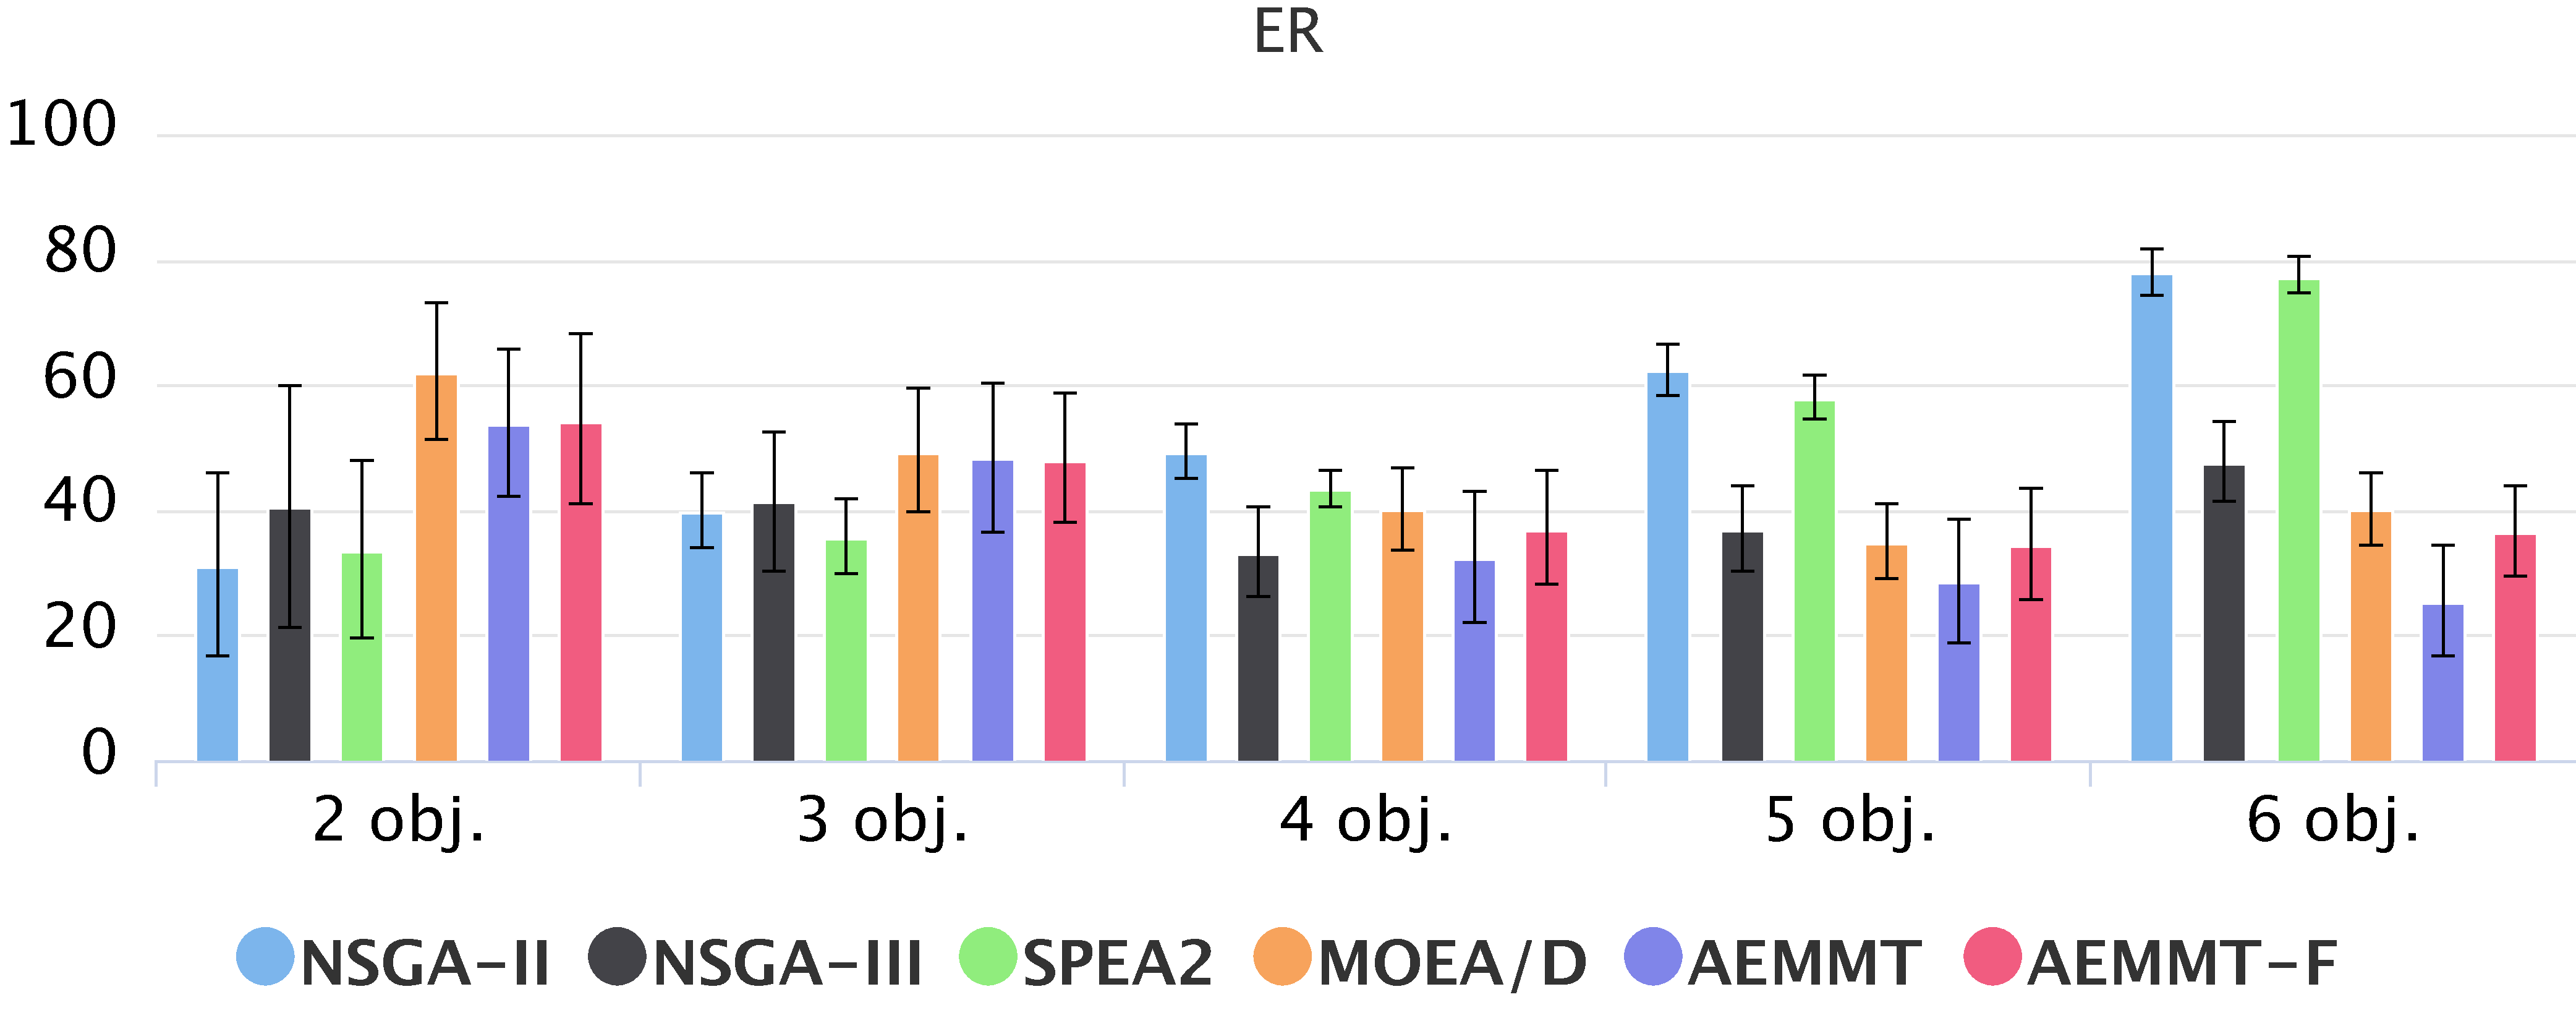
\includegraphics[width=1\textwidth]{cap_experimentos/figs/etapa1/er-mkp-todos}
	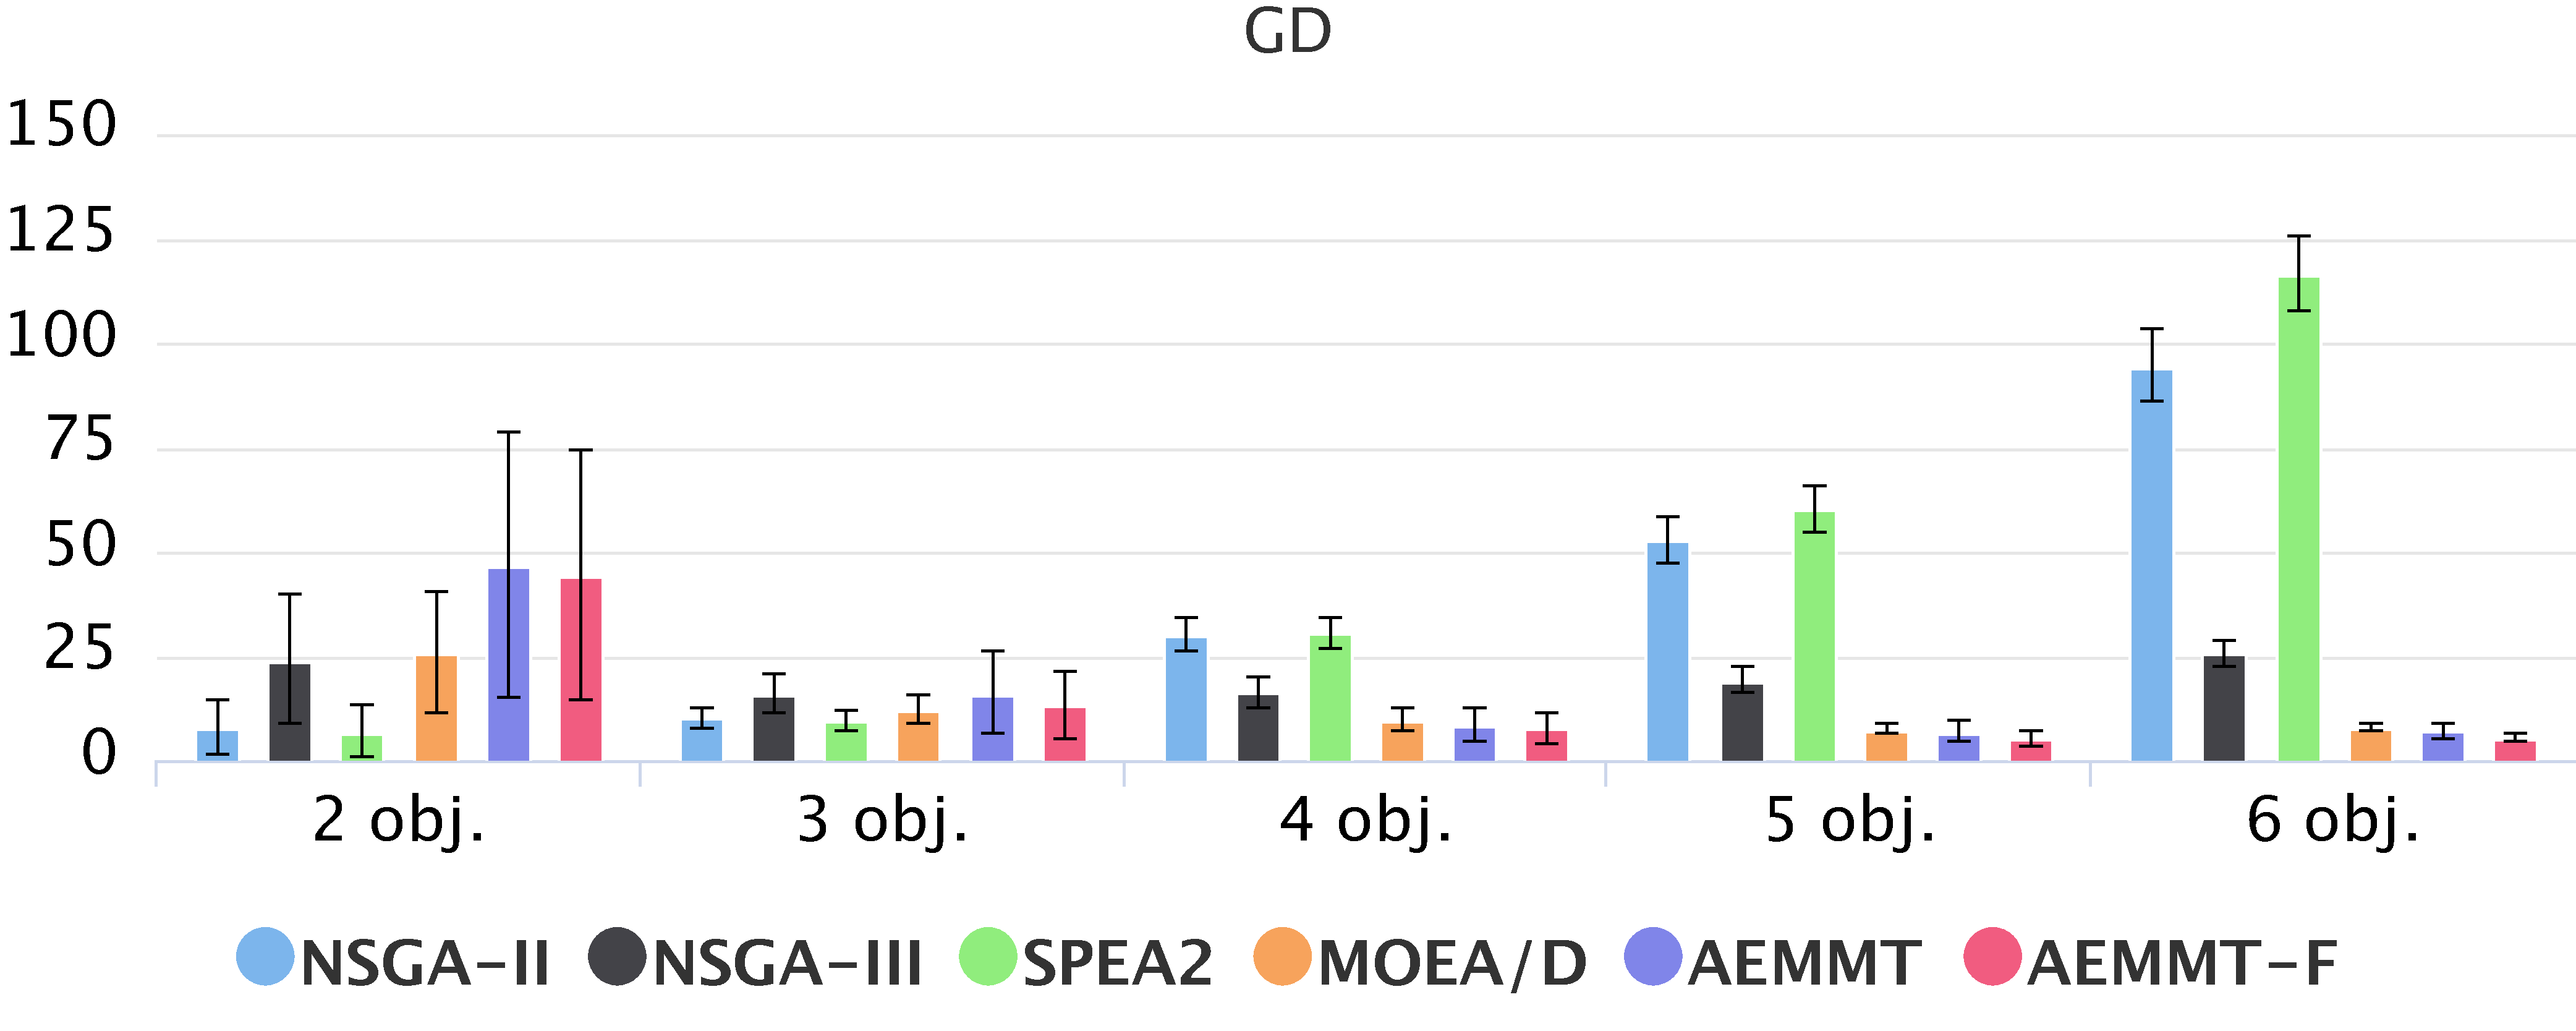
\includegraphics[width=1\textwidth]{cap_experimentos/figs/etapa1/gd-mkp-todos}
	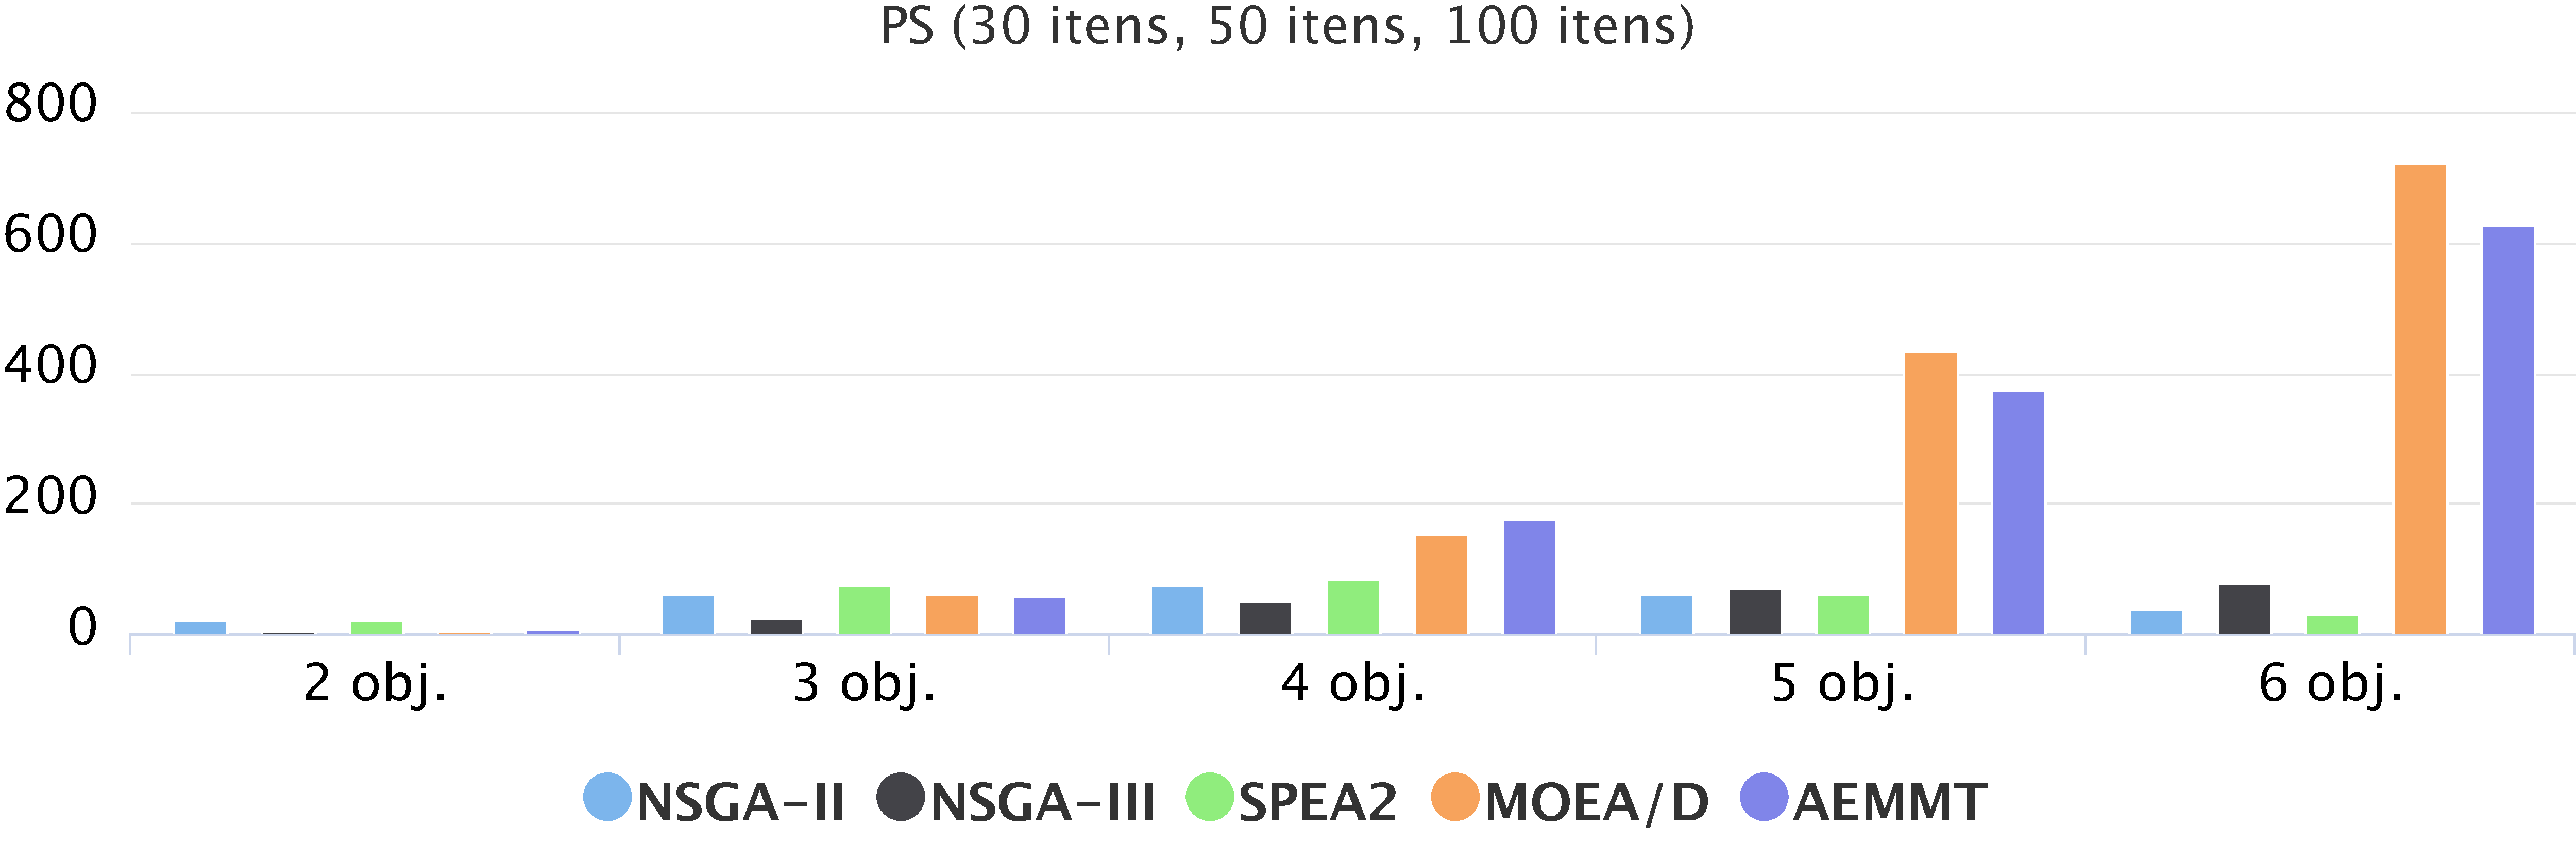
\includegraphics[width=1\textwidth]{cap_experimentos/figs/etapa1/ps-mkp-todos}
	\caption{\label{fig_exp1_pmm_todos}Resultado consolidado da 1ª etapa considerando o PMM com 30, 50 e 100 itens}
\end{figure*}

A \autoref{fig_exp1_pmm_todos} apresenta os resultados do PMM de 30, 50 e 100 itens de forma consolidada para que se possa analisar, de forma geral, o comportamento dos algoritmos nas diferentes formulações de objetivo. Os gráficos representam as médias (simples) entre os três cenários de dificuldade (30, 50 e 100 itens). Como esperado, o NSGA-II e o SPEA2 são os melhores algoritmos para as formulações de 2 e 3 objetivos, tendo resultado nos melhores valores para as métricas $ER$, $GD$ e $PS$. Por outro lado, a partir de 4 objetivos, o desempenho de ambos os algoritmos cai consideravelmente, enquanto o AEMMT passa a apresentar os melhores resultados. O NSGA-III, no problema de 4 objetivos, apresenta um erro quase tão baixo quanto o AEMMT, mas seu $GD$ e $PS$ são piores. O MOEA/D, para 5 e 6 objetivos, apresenta o segundo melhor desempenho em qualquer uma das métricas. Em resumo, o NSGA-III não parece uma boa opção em nenhum dos casos, pois sempre há outro algoritmo que o supera. O NSGA-II e o SPEA2 são igualmente bons e os melhores em problemas com poucos objetivos. O AEMMT e o MOEA/D são ótimas opções para problemas a partir de 4 objetivos, sendo que o MOEA/D confere um melhor $PS$ enquanto o AEMMT proporciona uma menor taxa de erro.

\begin{figure*}[!htbp]
	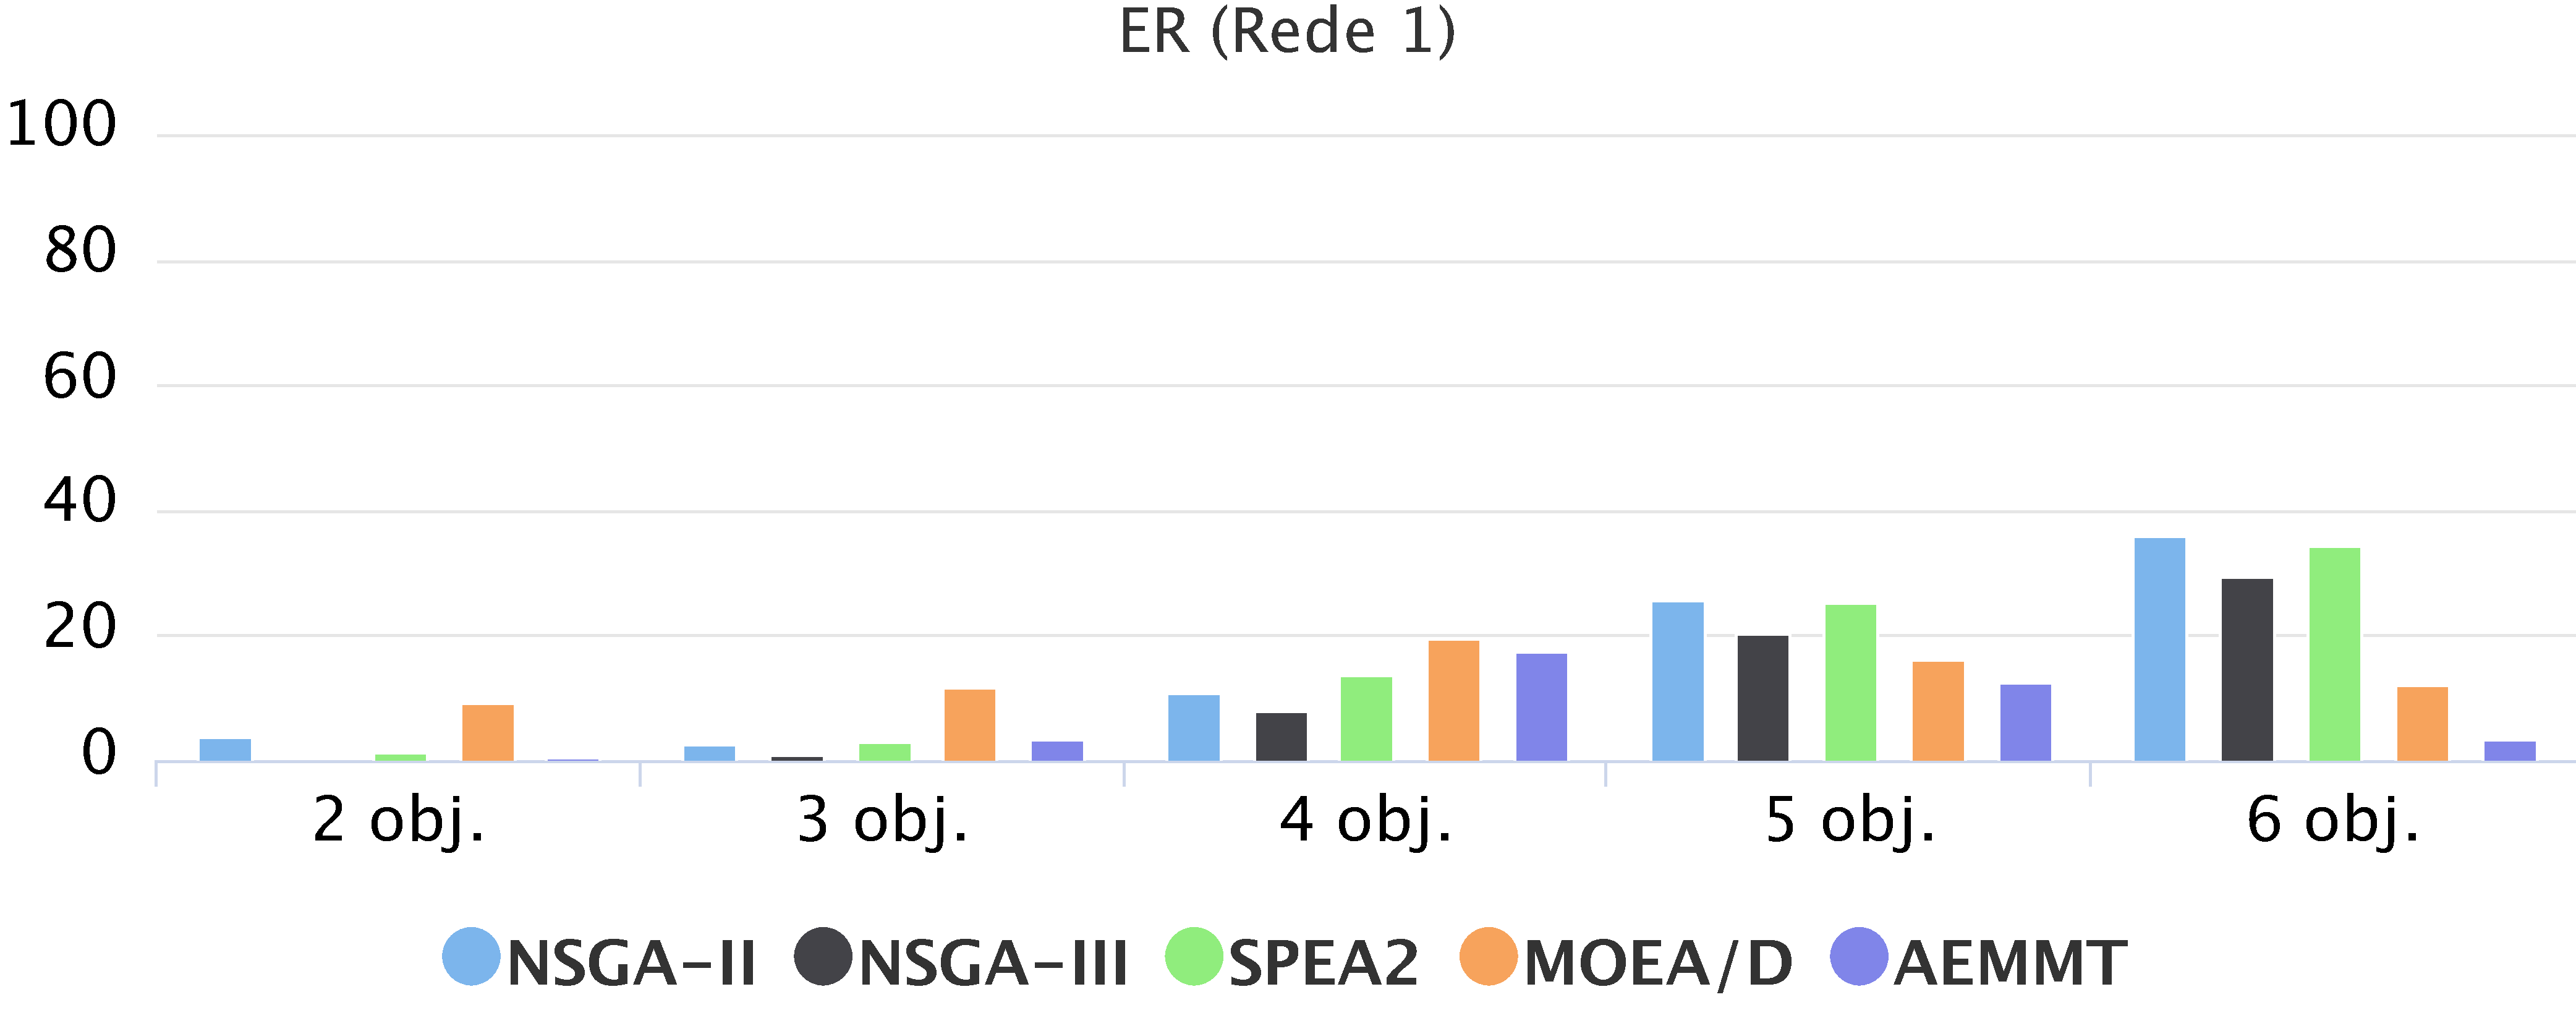
\includegraphics[width=1\textwidth]{cap_experimentos/figs/etapa1/er-mrp-r1}
	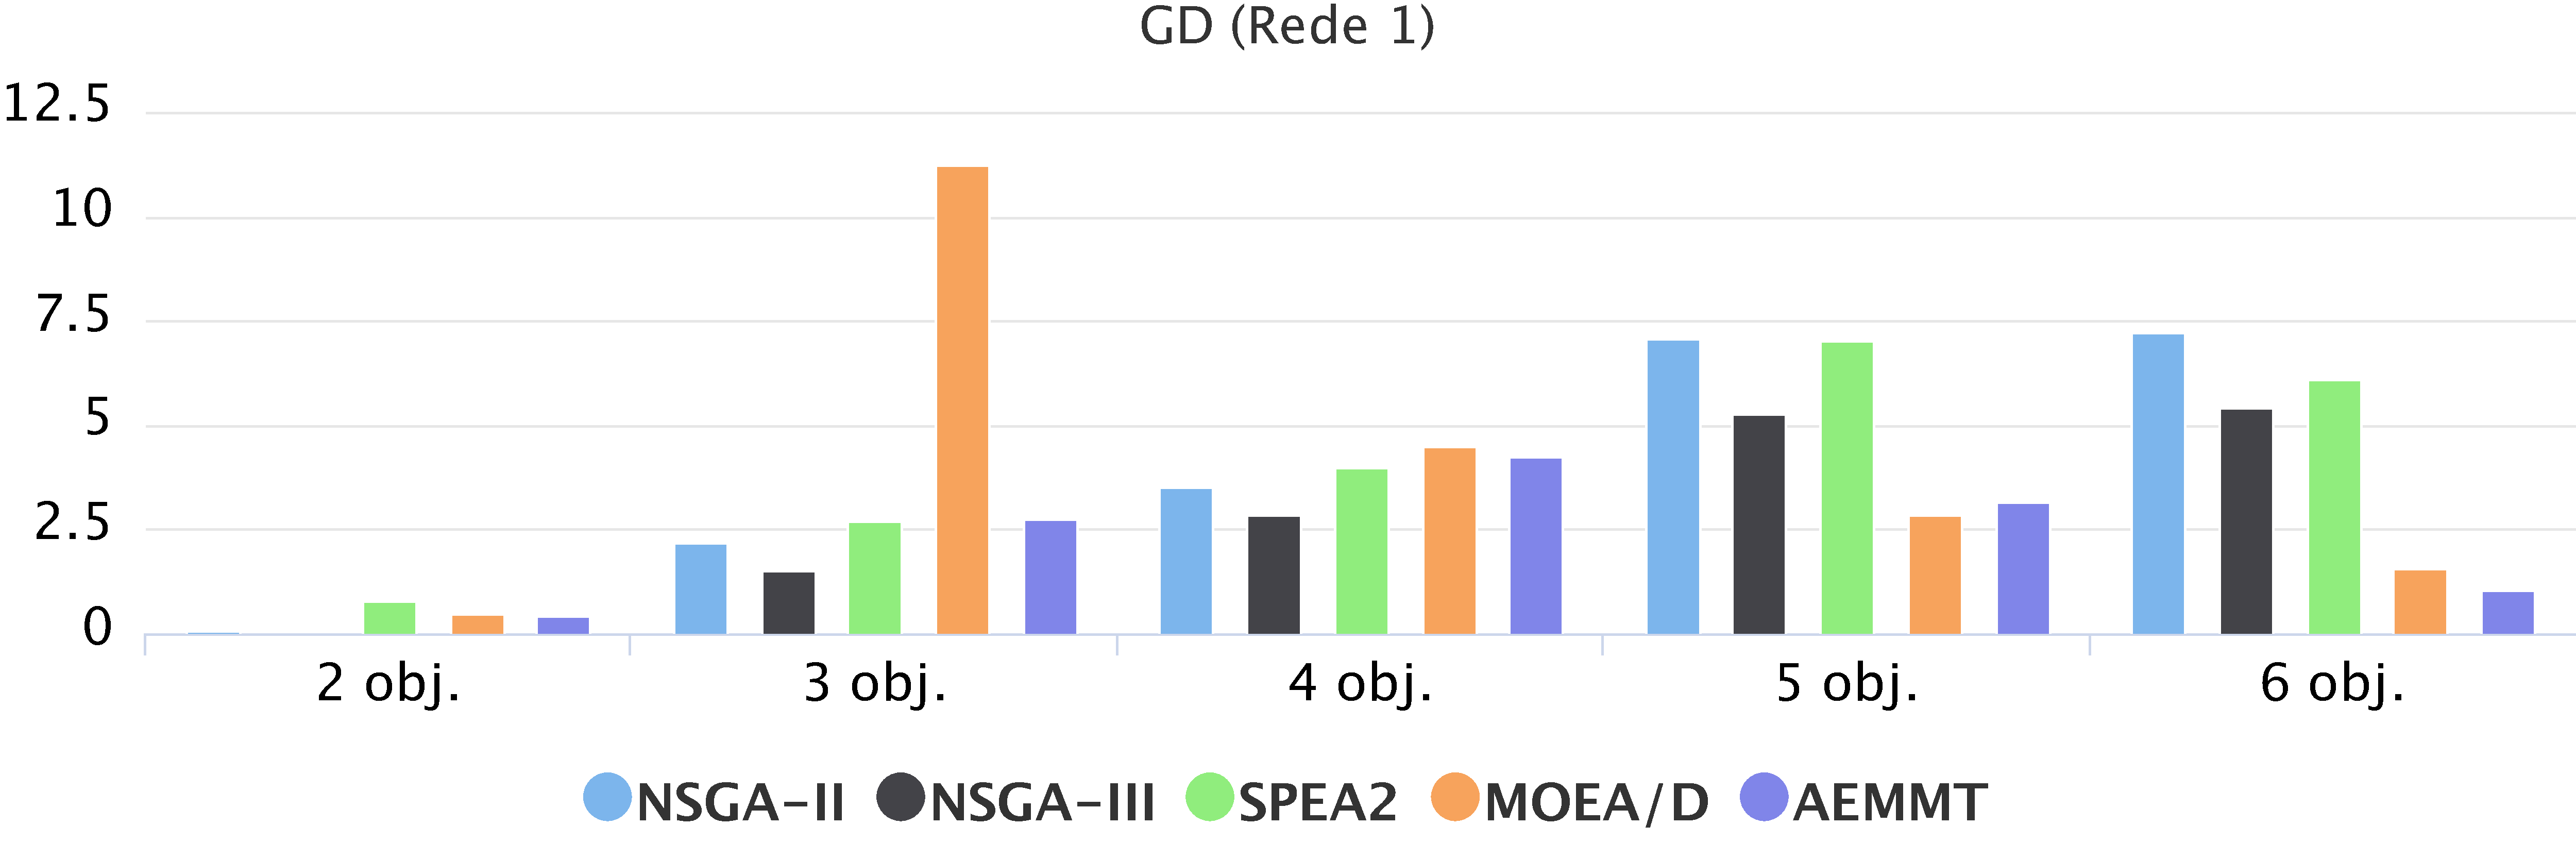
\includegraphics[width=1\textwidth]{cap_experimentos/figs/etapa1/gd-mrp-r1}
	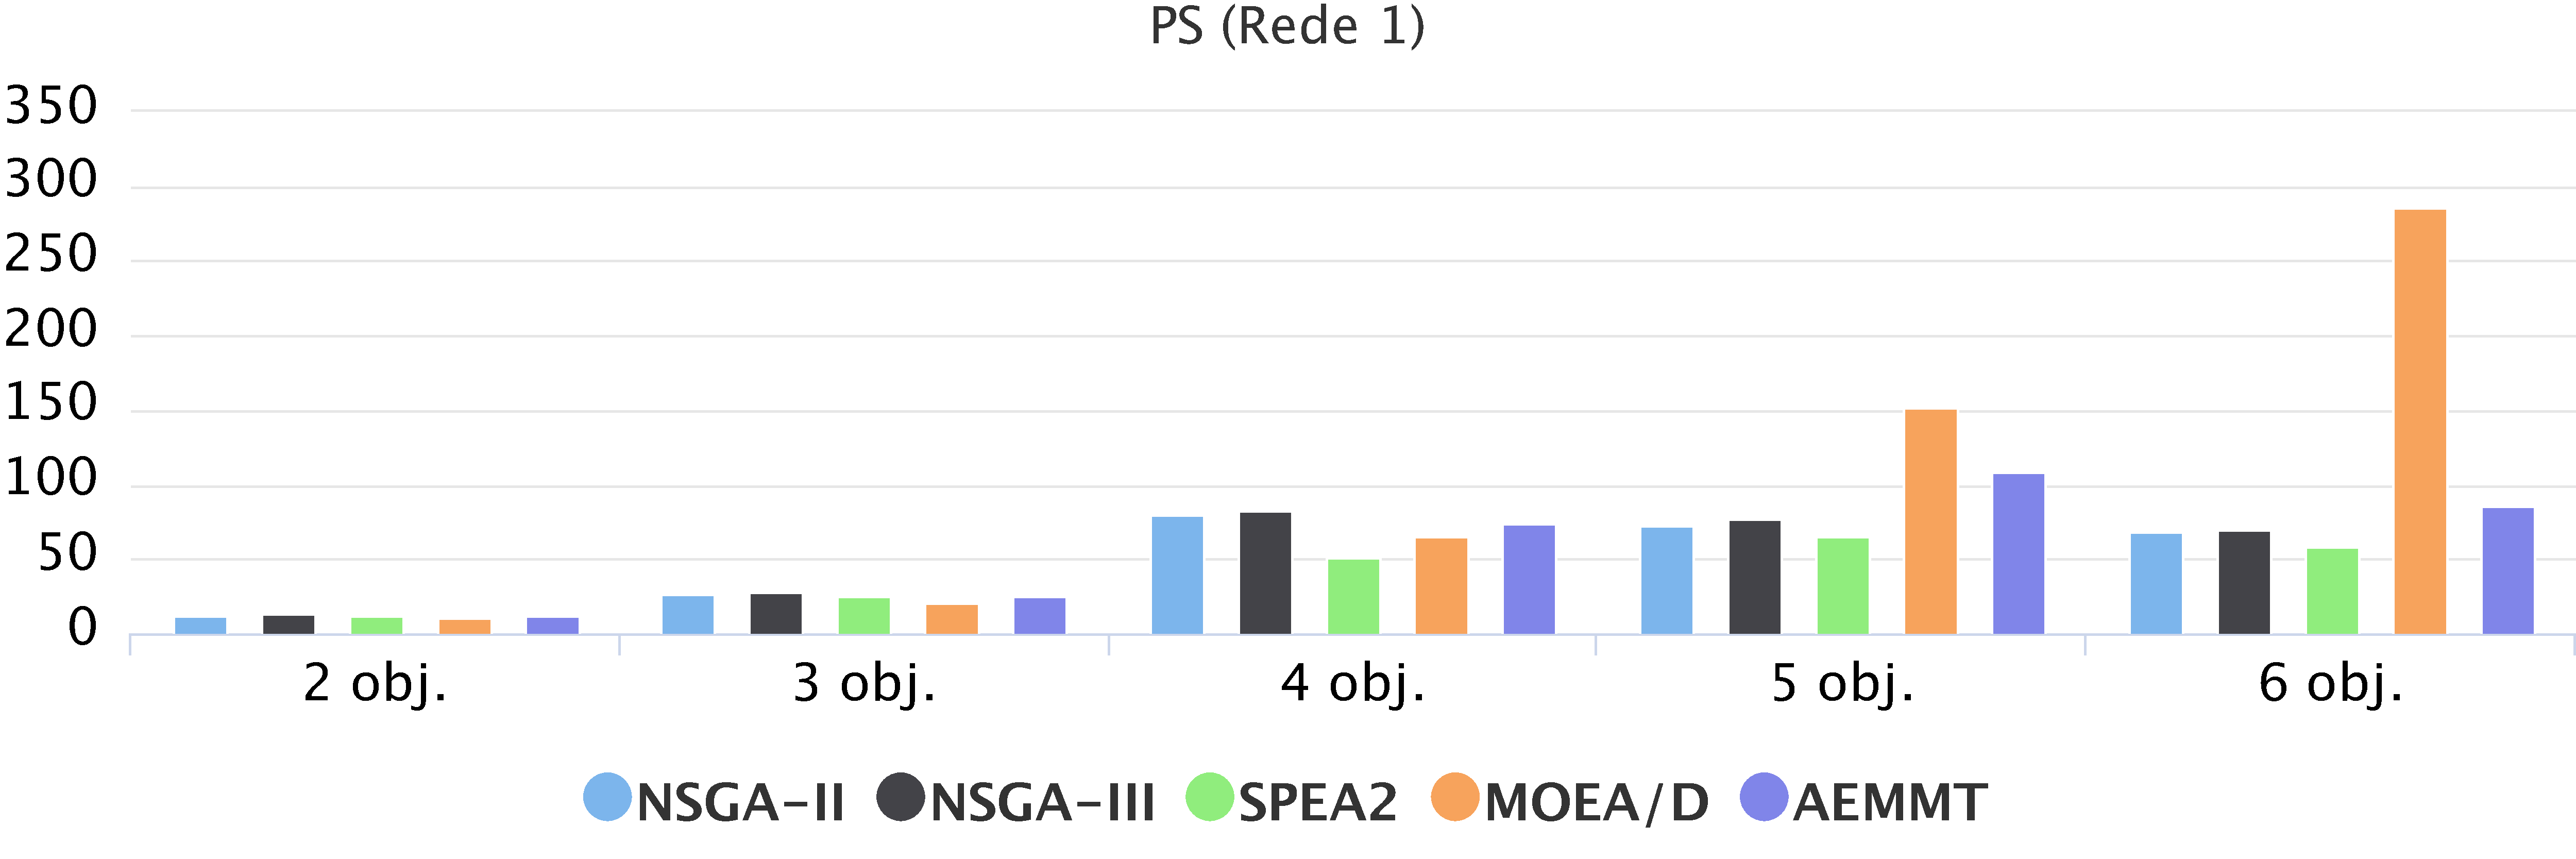
\includegraphics[width=1\textwidth]{cap_experimentos/figs/etapa1/ps-mrp-r1}
	\caption{\label{fig_exp1_prm_r1}Desempenho dos algoritmos na 1ª etapa para o PRM na rede 1}
\end{figure*}

Na \autoref{fig_exp1_prm_r1} são apresentados os desempenhos dos AEMOs na resolução do PRM para a rede 1. Essa é a instância mais simples testada e retornou baixas taxas de erro para todos os algoritmos. Considerando todas as formulações de objetivo, o maior valor de $ER$ foi obtido pelo NSGA-II aplicado ao problema de 6 objetivos (36,3\%). Diferentemente do esperado, o NSGA-III mostrou o melhor resultado ($ER$, $GD$ e $PS$) para os problemas com 2, 3 e 4 objetivos. A partir de 5 objetivos, o AEMMT e o MOEA/D são os dois melhores métodos, sendo que o primeiro apresenta uma menor taxa de erro, enquanto o segundo obtém uma fronteira de soluções não-dominadas de maior cardinalidade. Para poucos objetivos, o NSGA-III é claramente o melhor método, para 5 ou mais critérios de otimização, ambos AEMMT e MOEA/D são boas opções.

\begin{figure*}[!htbp]	
	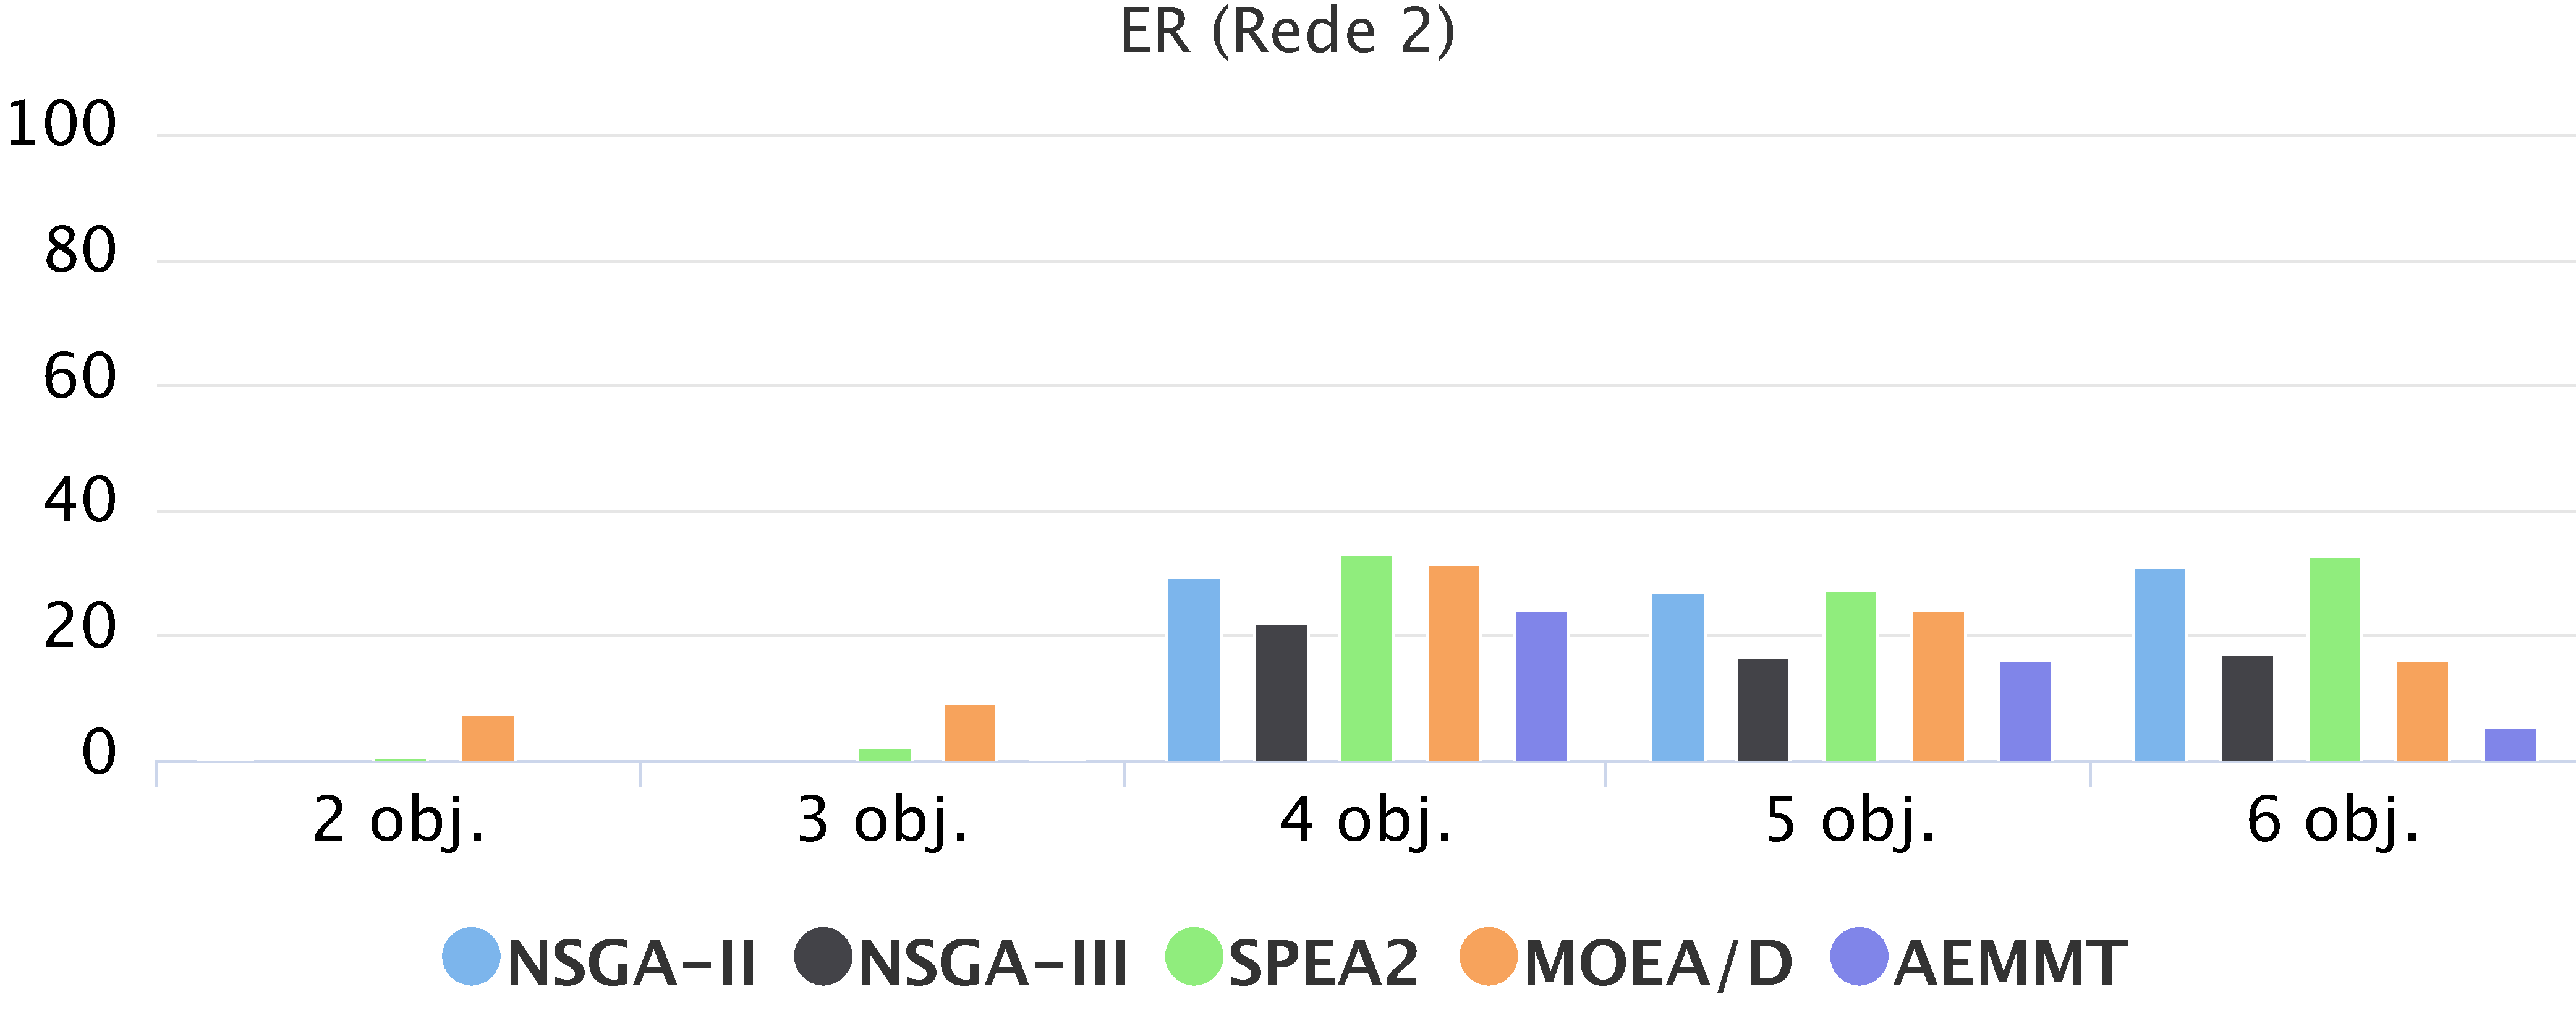
\includegraphics[width=1\textwidth]{cap_experimentos/figs/etapa1/er-mrp-r2}
	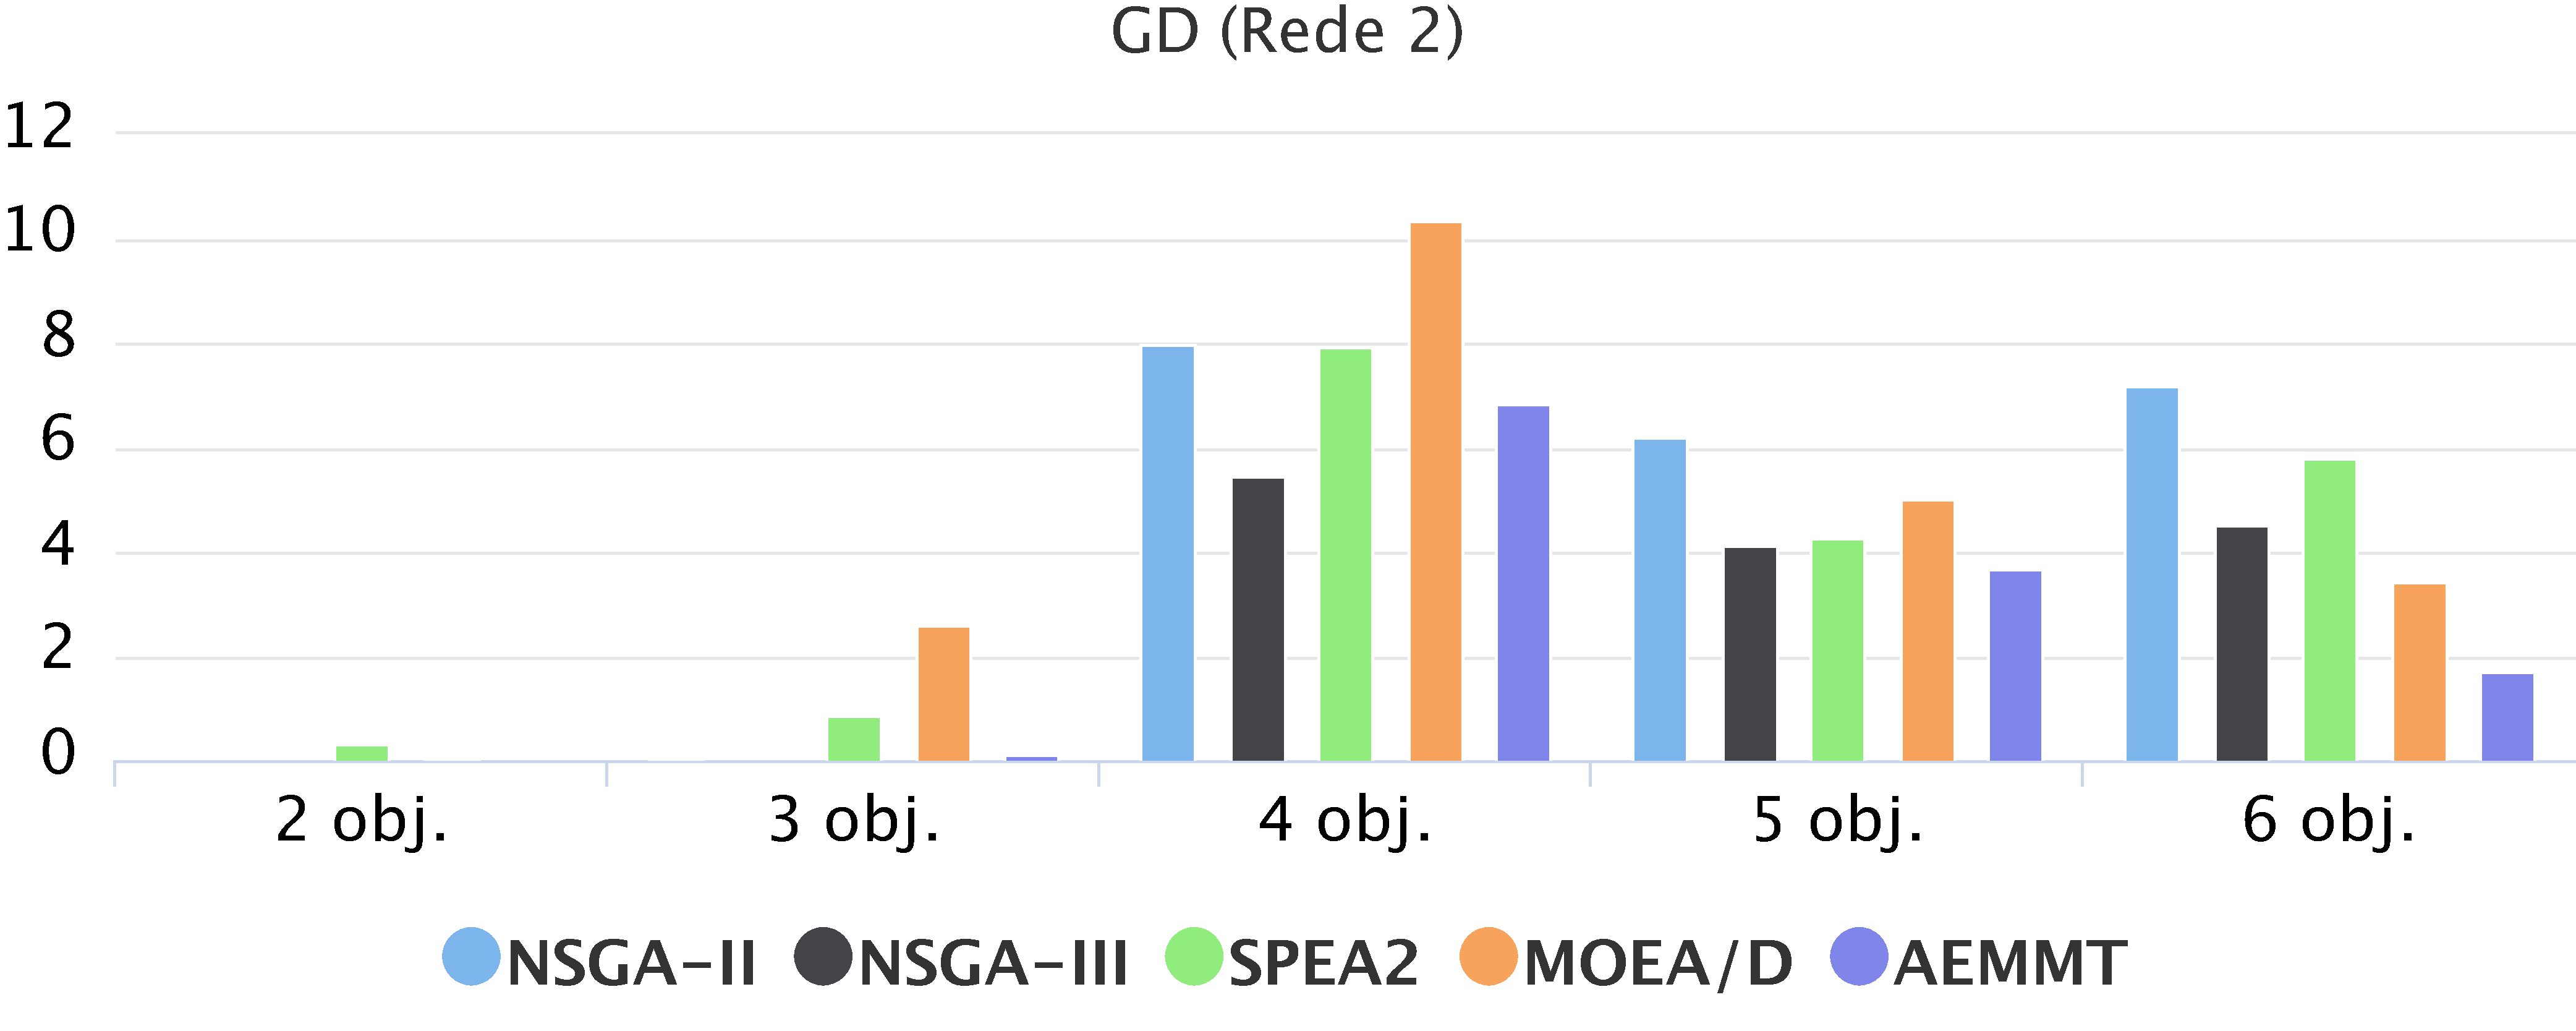
\includegraphics[width=1\textwidth]{cap_experimentos/figs/etapa1/gd-mrp-r2}
	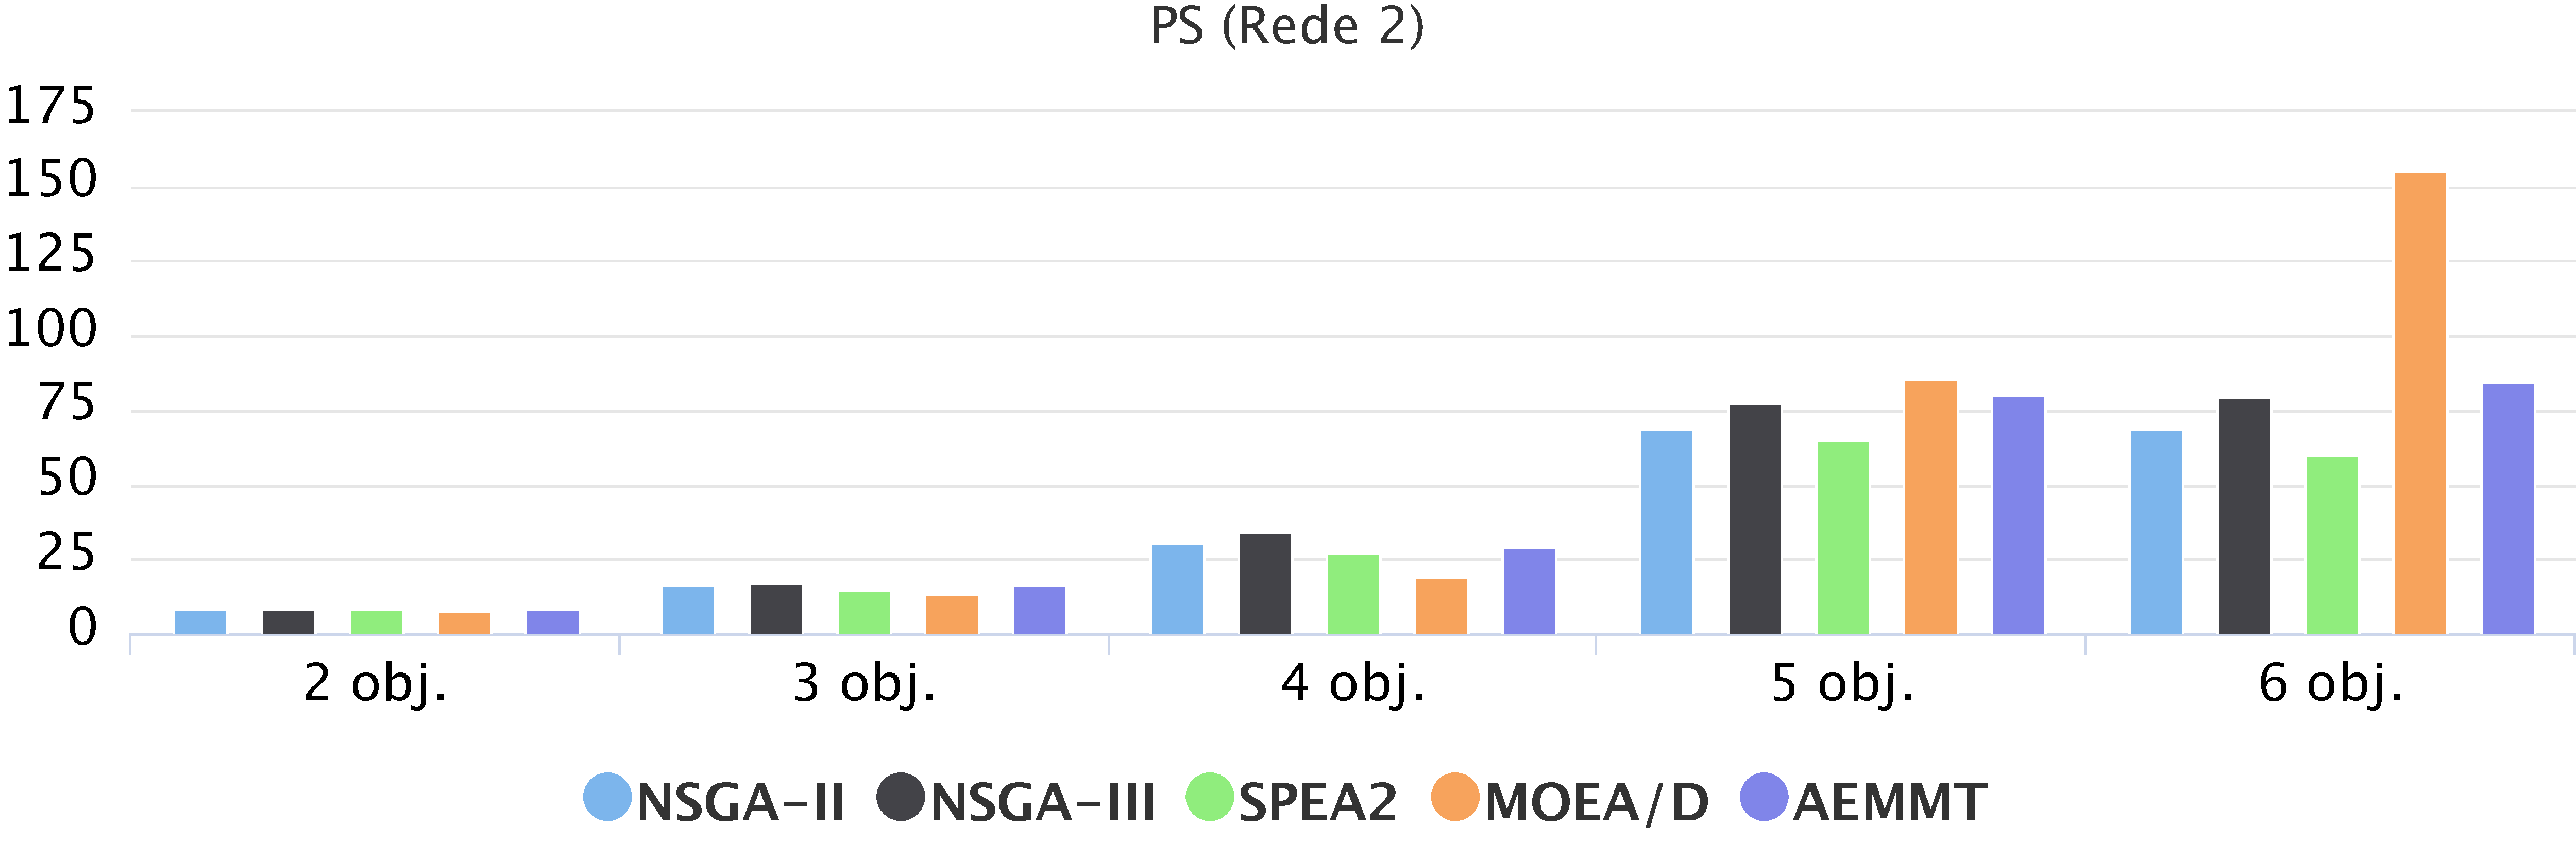
\includegraphics[width=1\textwidth]{cap_experimentos/figs/etapa1/ps-mrp-r2}
	\caption{\label{fig_exp1_prm_r2}Desempenho dos algoritmos na 1ª etapa para o PRM na rede 2}
\end{figure*}

Considerando o desempenho dos AEMOs para o PRM com a rede 2 (\autoref{fig_exp1_prm_r2}), o NSGA-III é o melhor algoritmo nos problemas com 2, 3 e 4 objetivos, em qualquer uma das métricas, seguido pelo NSGA-II e SPEA2. Para 5 objetivos, o AEMMT apresenta a menor taxa de erro (16,6\%), seguido de perto pelo NSGA-III (16,9\%). Com relação ao $GD$ no problema de 5 objetivos, o AEMMT obtém o melhor desempenho, mas o NSGA-III e o SPEA2 atingem valores similares. Em termos de $PS$, o MOEA/D, o AEMMT e o NSGA-III conseguem valores bem similares, sendo o MOEA/D o melhor dentre eles. Para 6 objetivos, os menores $ER$ e $GD$ foram obtidos pelo AEMMT (3,6\%; 1,7), em primeiro lugar, pelo MOEA/D (16,3\%; 3,4), em segundo e pelo NSGA-III (17,4\%; 4,5), em terceiro. Os melhores valores de $PS$ foram apresentados pelo MOEA/D (155,4), que ficou bem a frente dos segundo e terceiro melhores algoritmos (AEMMT com 84,8 e NSGA-III com 79,9). Nos cenários com poucos objetivos, o NSGA-III mostrou ser a melhor opção para a rede 2, enquanto nos com 5 ou mais objetivos, é preferível utilizar o AEMMT, caso uma baixa taxa de erro seja desejável, ou o MOEA/D, caso deseja-se um maior conjunto de soluções não-dominadas.

\begin{figure*}[!htbp]
	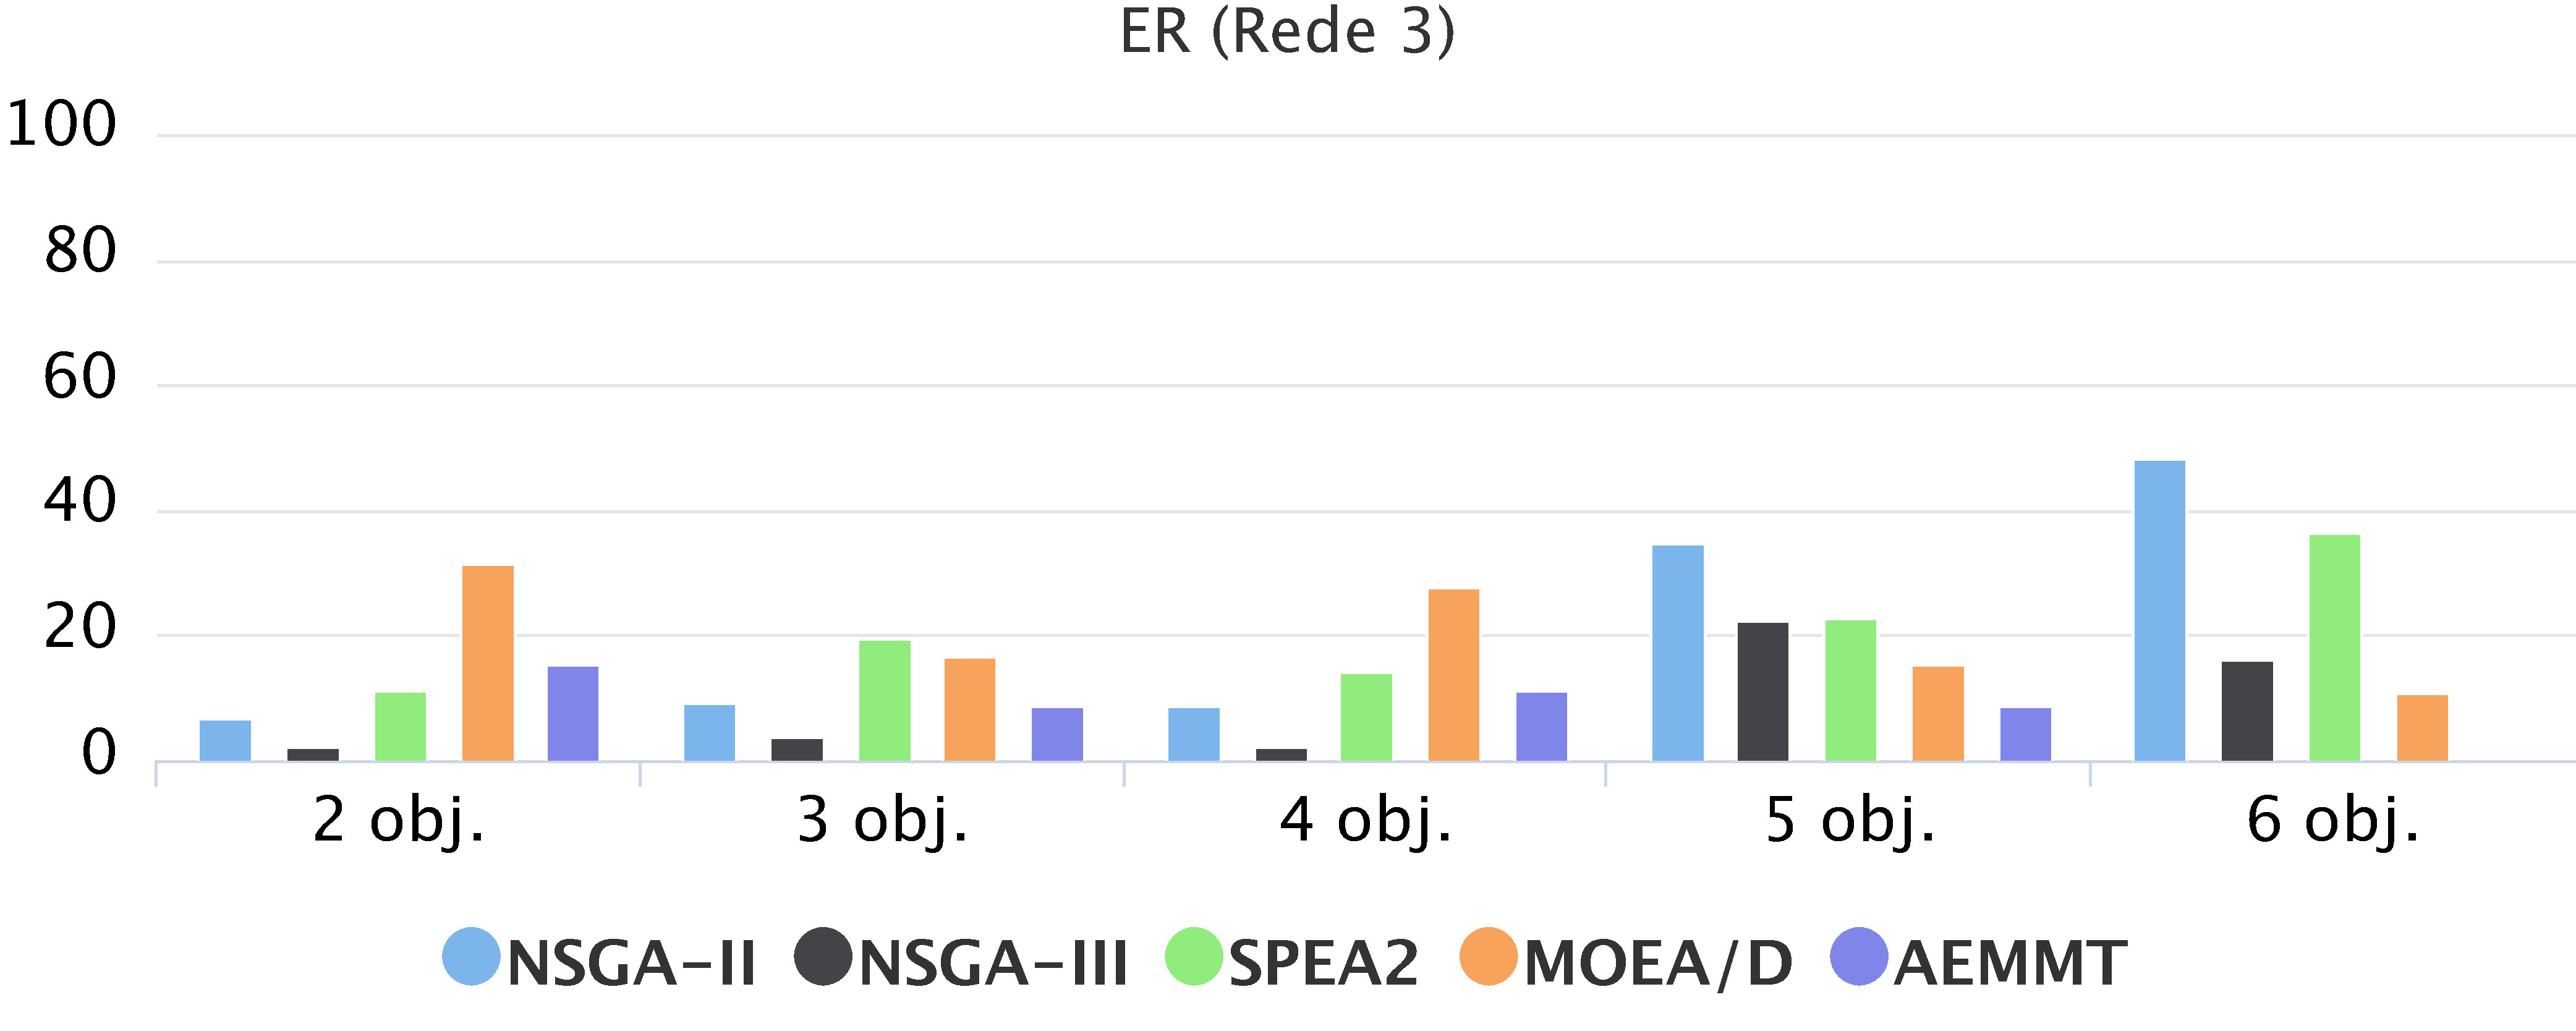
\includegraphics[width=1\textwidth]{cap_experimentos/figs/etapa1/er-mrp-r3}
	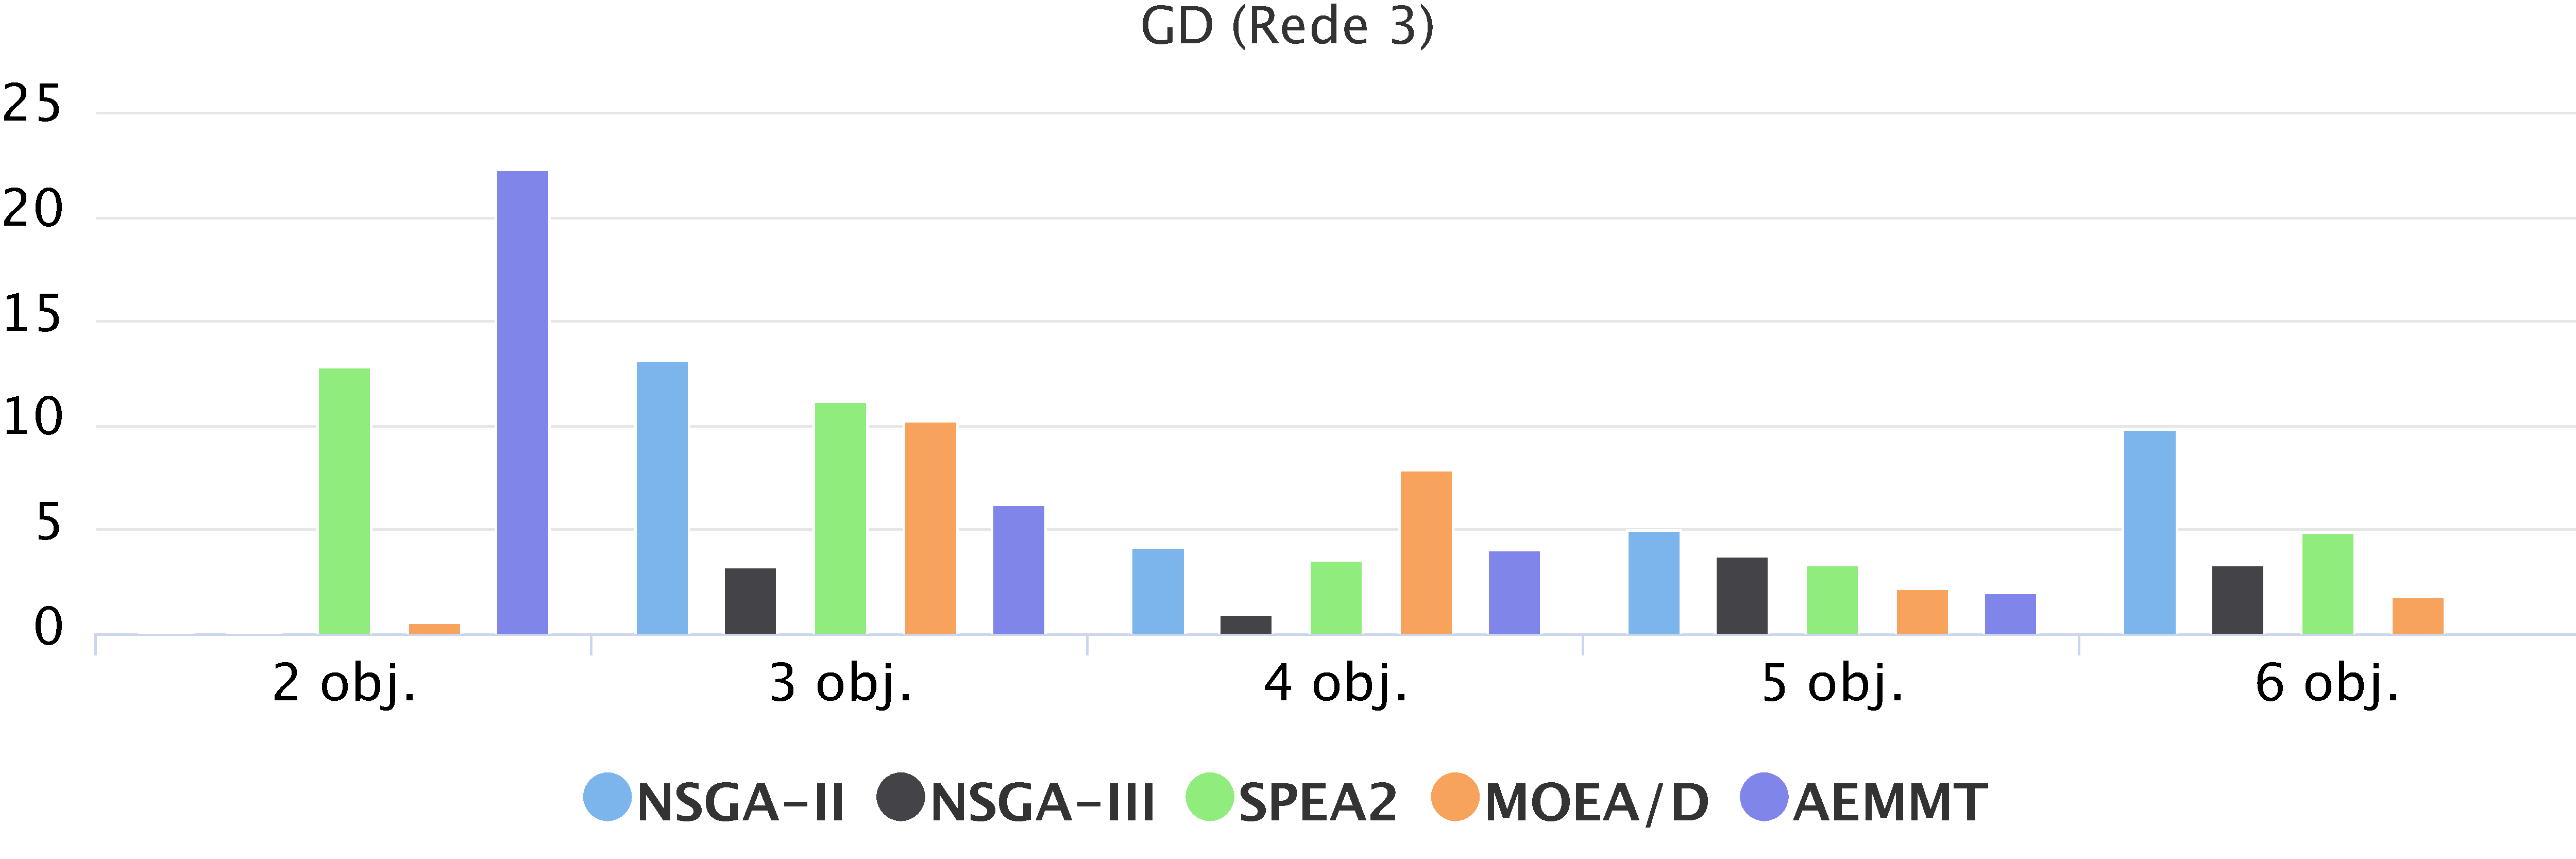
\includegraphics[width=1\textwidth]{cap_experimentos/figs/etapa1/gd-mrp-r3}
	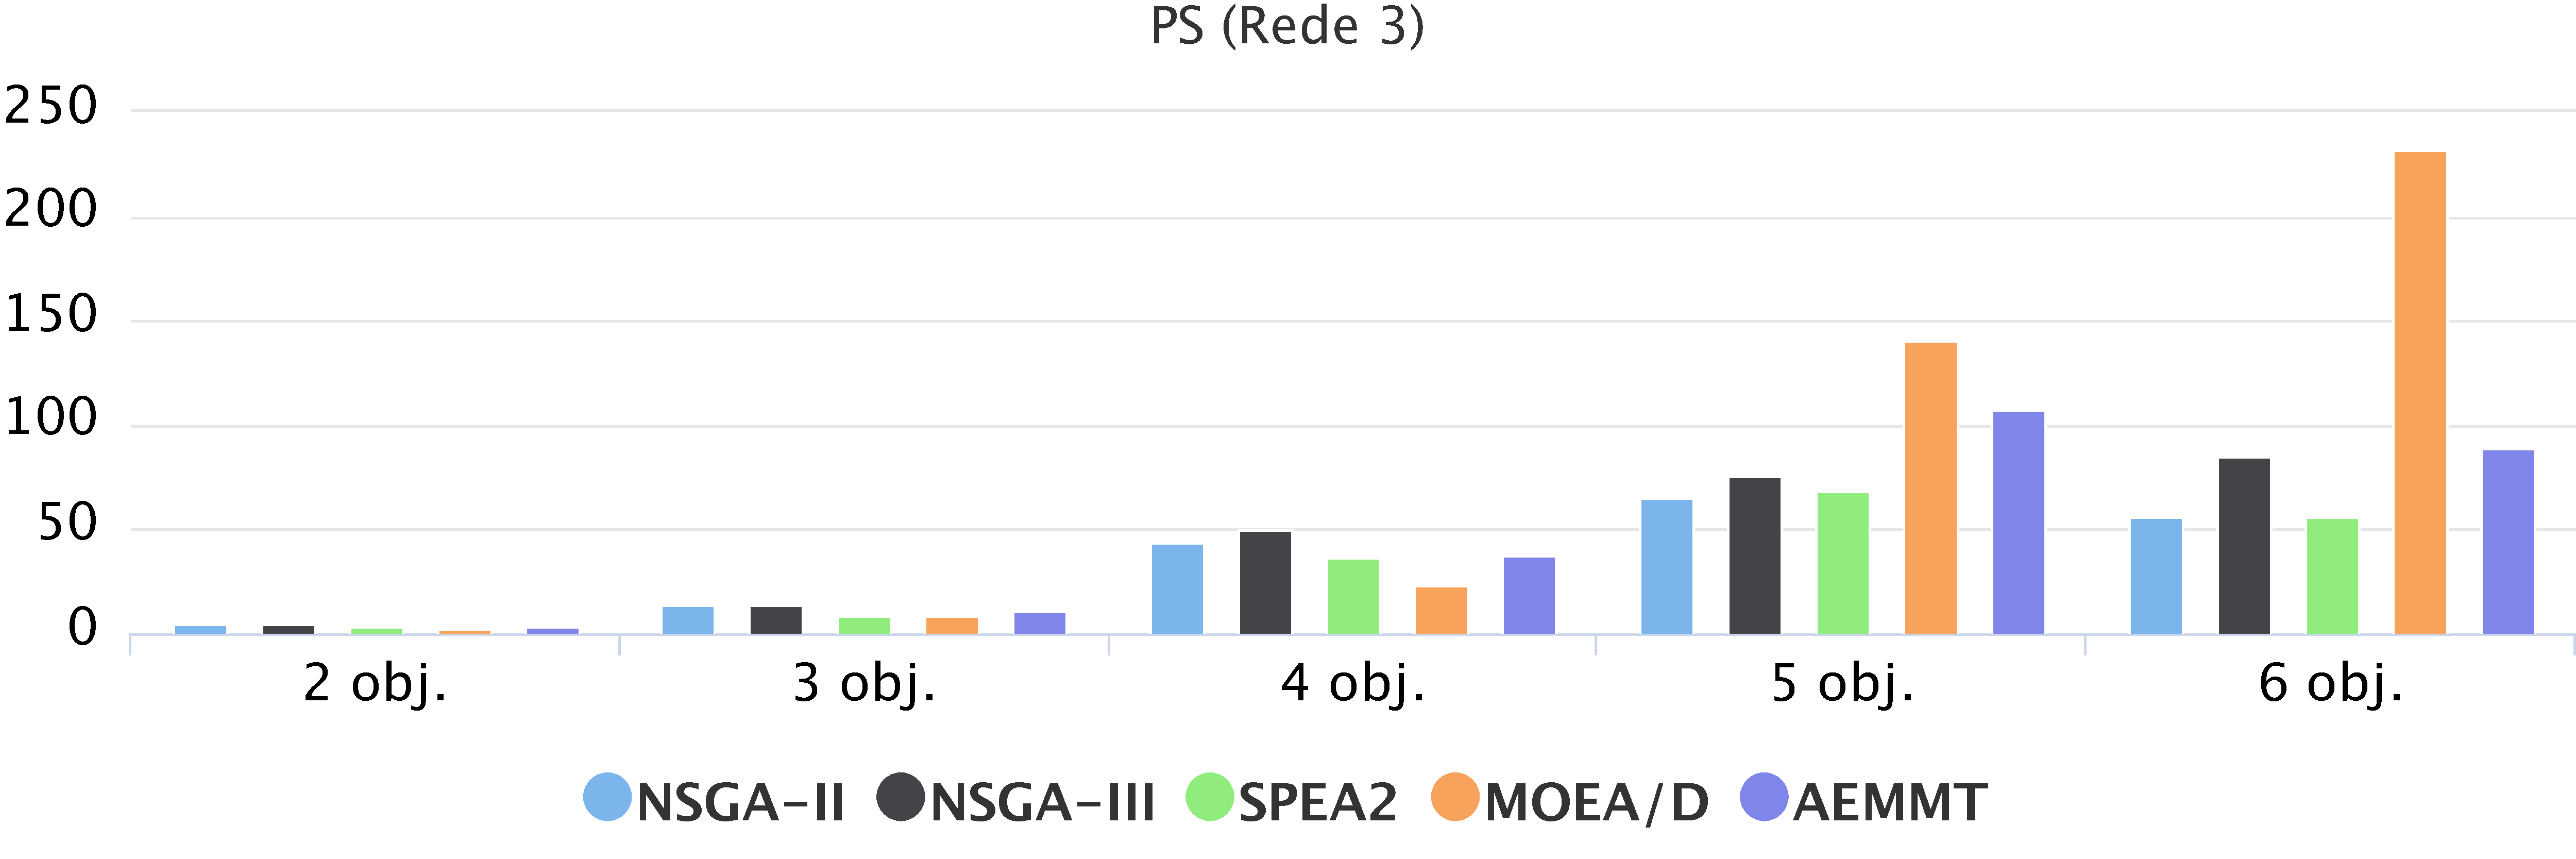
\includegraphics[width=1\textwidth]{cap_experimentos/figs/etapa1/ps-mrp-r3}
	\caption{\label{fig_exp1_prm_r3}Desempenho dos algoritmos na 1ª etapa para o PRM na rede 3}
\end{figure*}

A rede 3 é a mais complexa analisada nesta etapa dos experimentos. Analisando-se os resultados dos gráficos apresentados na \autoref{fig_exp1_prm_r3}, a tendência já observada nas demais instâncias é mantida, na qual o NSGA-III continua sendo o melhor método para as formulações com poucos objetivos. Até 4 objetivos, em todas as métricas, o NSGA-III apresenta os melhores resultados. Para 5 e 6 objetivos, o AEMMT apresenta menor $ER$ e $GD$, enquanto o MOEA/D consegue maior $PS$.

\begin{figure*}[!htbp]	
	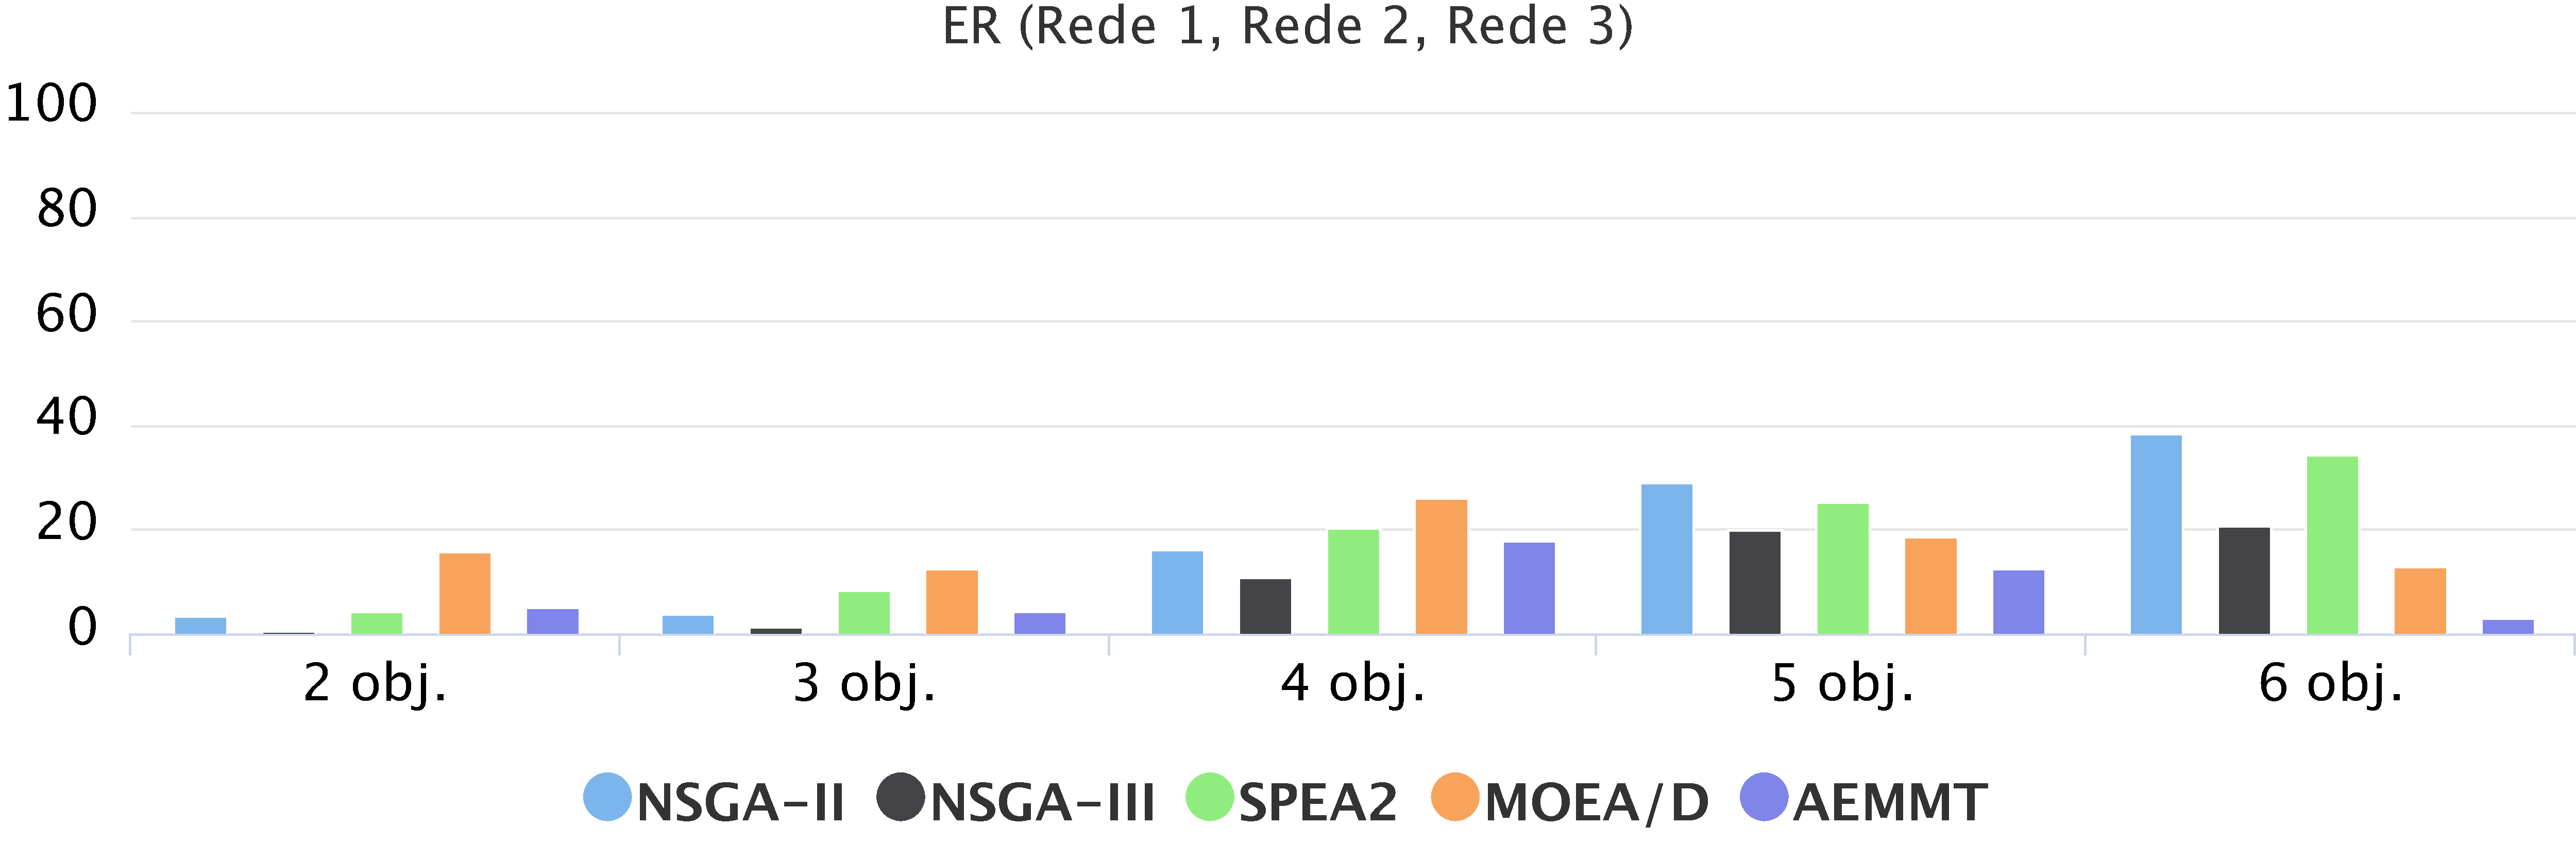
\includegraphics[width=1\textwidth]{cap_experimentos/figs/etapa1/er-mrp-todos}
	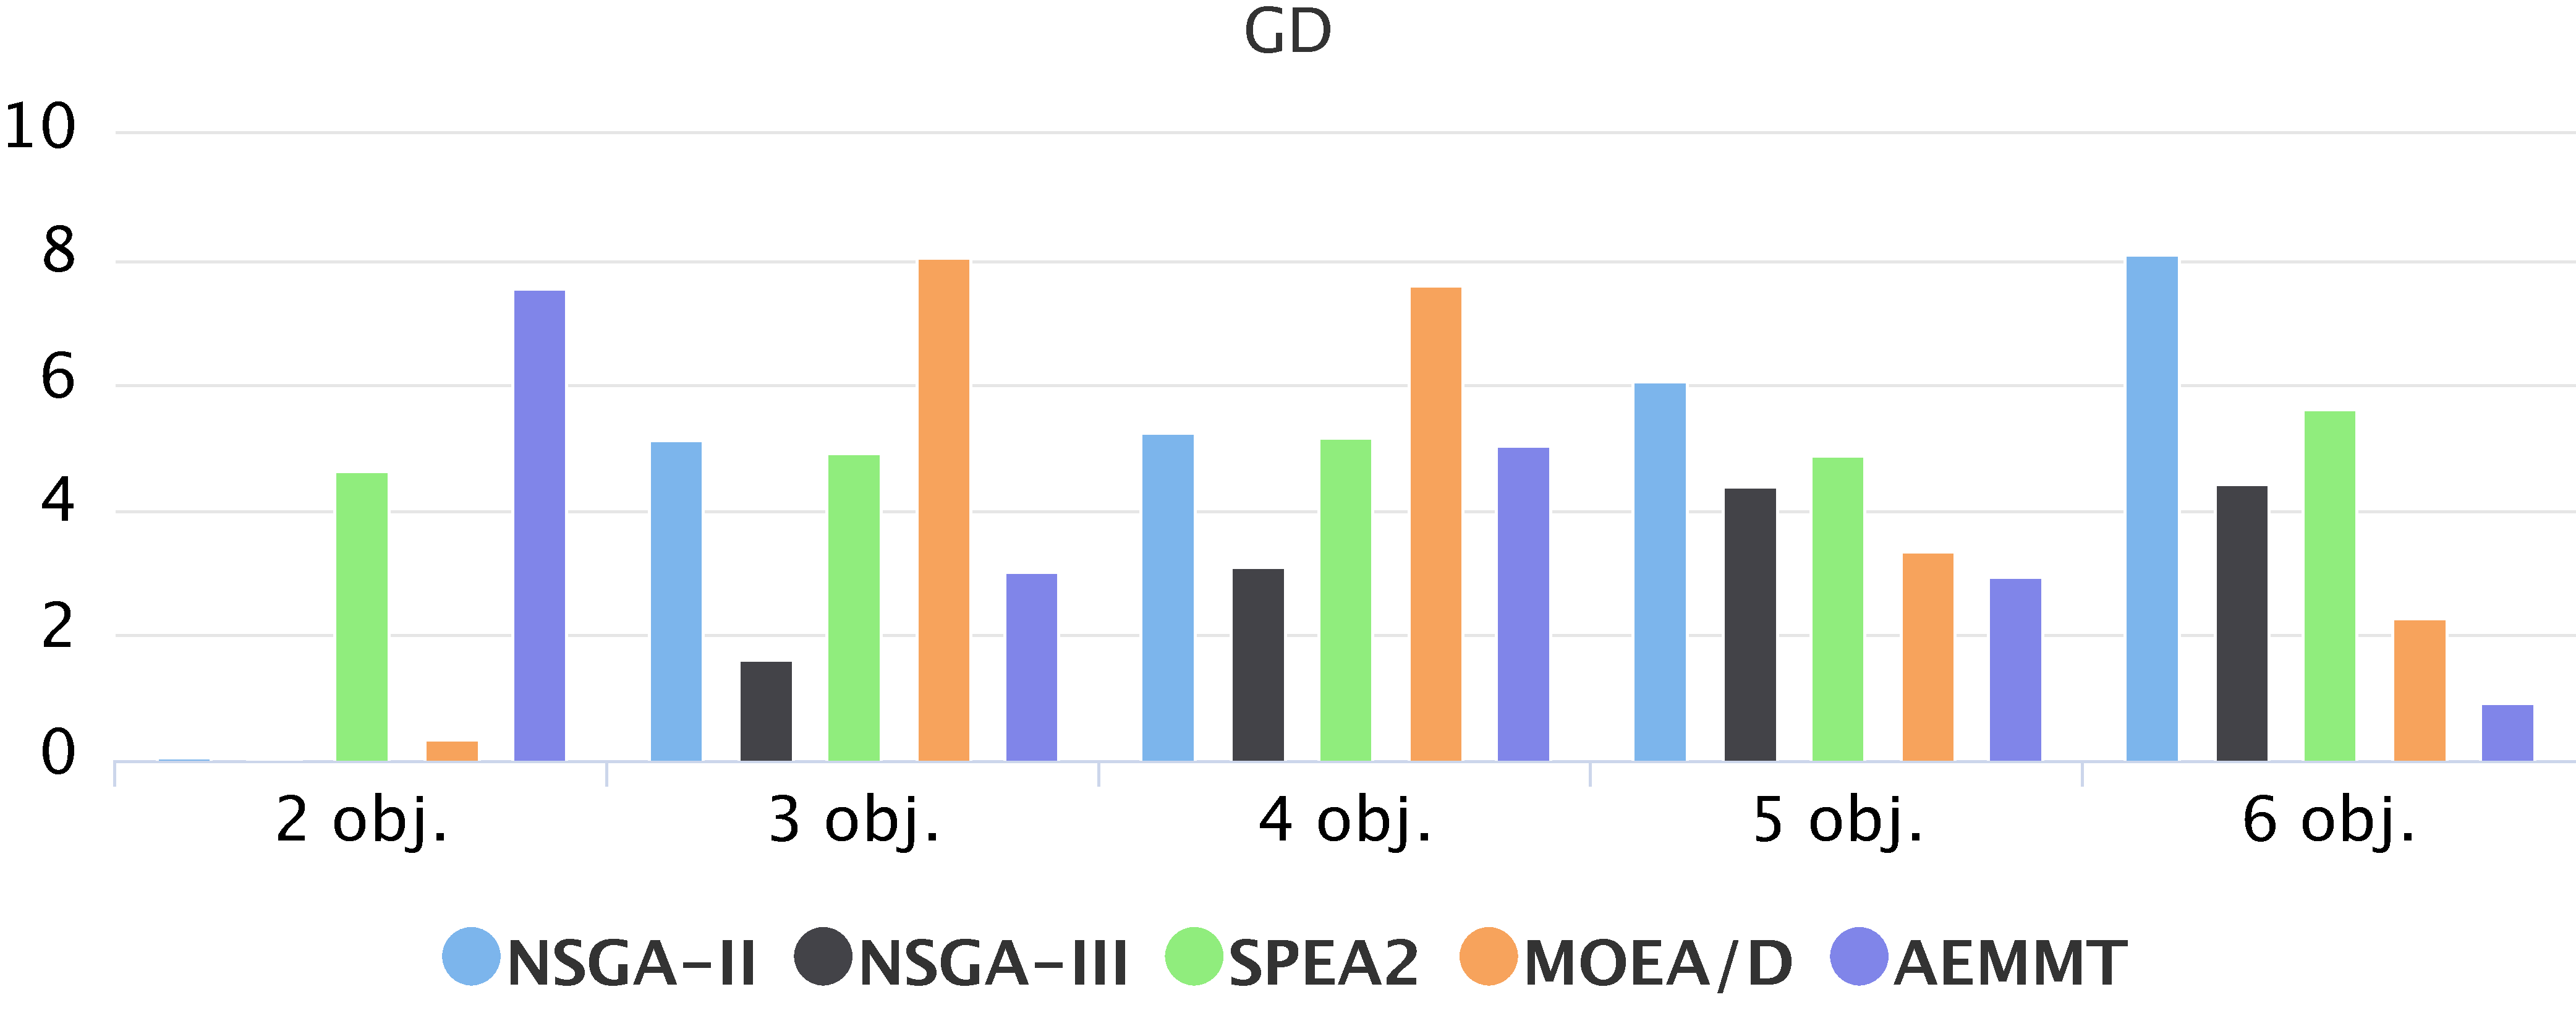
\includegraphics[width=1\textwidth]{cap_experimentos/figs/etapa1/gd-mrp-todos}
	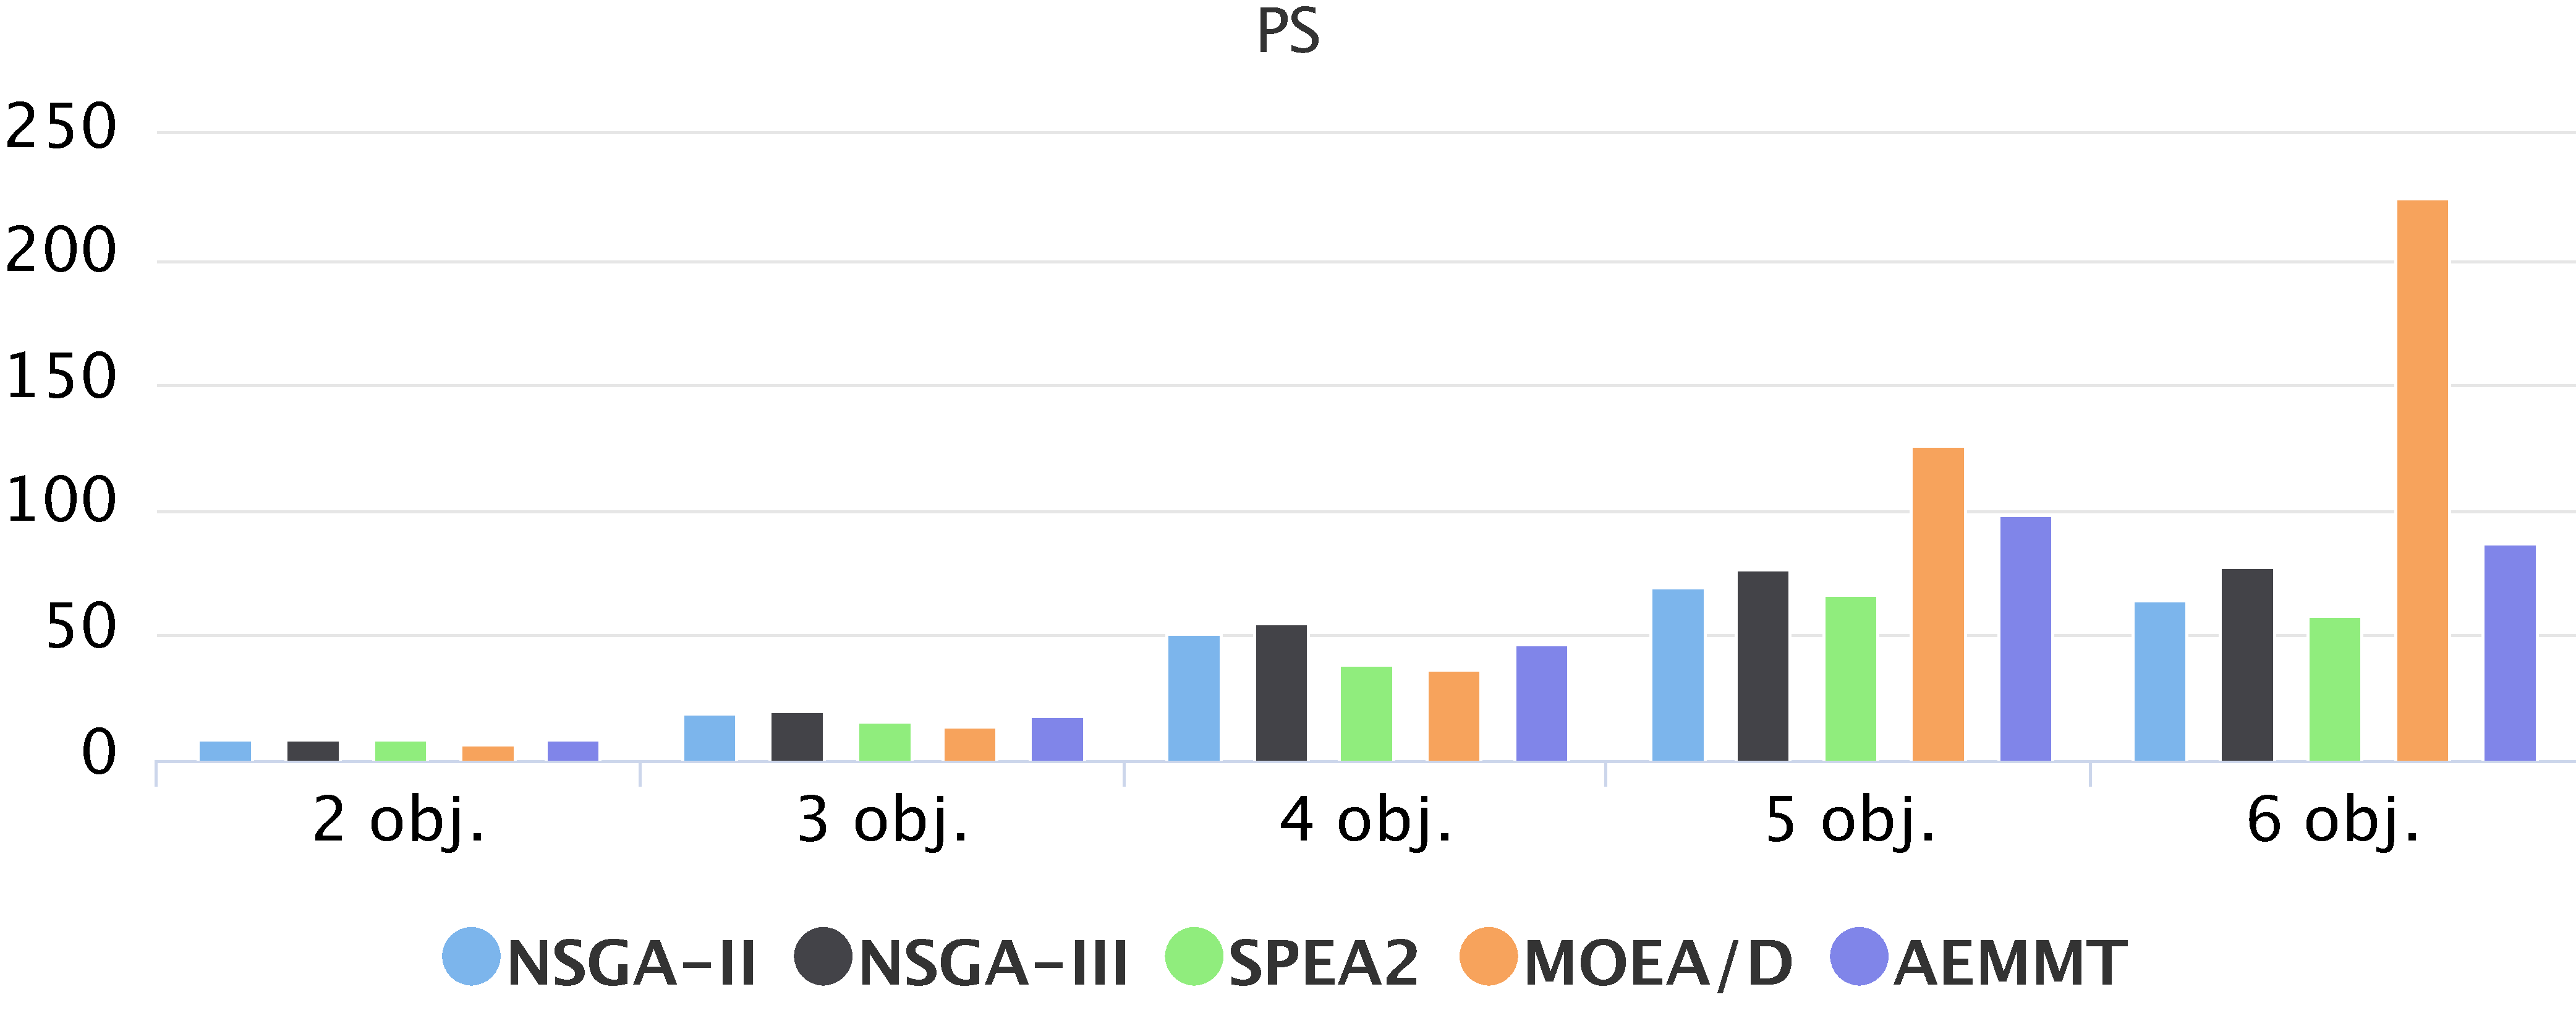
\includegraphics[width=1\textwidth]{cap_experimentos/figs/etapa1/ps-mrp-todos}
	\caption{\label{fig_exp1_prm_todos}Resultado consolidado da 1ª etapa considerando o PRM nas redes 1, 2, e 3}
\end{figure*}

A fim de fazer uma análise geral do PRM, os desempenhos dos algoritmos em todas as instâncias do problema (redes 1, 2 e 3) são consolidados nos gráficos da \autoref{fig_exp1_prm_todos}. Assim como no PMM, essa consolidação é obtida através da média aritmética dos valores das métricas em cada instância. Apesar de ser esperado que o NSGA-II e o SPEA2 fossem os melhores métodos para poucos objetivos, a partir dos gráficos da \autoref{fig_exp1_prm_todos}, observa-se que o NSGA-III obteve o melhor resultado para as formulações com 2, 3 e 4 objetivos. O NSGA-II também atinge bons resultados para 2 e 3 objetivos, mas o SPEA2 apresenta um $GD$ relativamente ruim. Considerando problemas de 5 e 6 objetivos, a escolha do algoritmo depende do intuito da busca. Se a quantidade encontrada de soluções do Pareto for mais relevante, o MOEA/D é mais indicado. Por outro lado, se um menor erro é preferível, então o AEMMT é a melhor opção.

Considerando-se ambos os problemas, PMM e PRM, os algoritmos NSGA-II, SPEA2 e NSGA-III são os que geram melhores resultados para problemas com poucos objetivos. O desempenho dos algoritmos clássicos (NSGA-II e SPEA2) diminui consideravelmente à medida que se aumenta o número de objetivos. Em contrapartida, o desempenho dos métodos AEMMT e MOEA/D melhora a partir de quatro objetivos, tornando-os mais indicados para problemas \textit{many-objectives}.

Outra observação que pôde ser feita a partir dos experimentos desta etapa é que o AEMMT perde apenas em $PS$ para o MOEA/D. Uma das características do AEMMT é a limitação no tamanho da tabela de não dominância (arquivo com os indivíduos não dominados), o que levanta a seguinte questão: se não houvesse esse limite, o AEMMT alcançaria melhor resultado em todas as métricas? Visando responder tal questão, foram executados novos experimentos para avaliar o desempenho de uma variação do AEMMT (AEMMT-F), na qual não existe um limite para o tamanho da tabela de não dominância. Na maioria dos experimentos, o AEMMT-F apresentou uma taxa de erro maior que sua versão original. Em contrapartida, essa variação alcançou valores médios para as métricas $ER$ e $PS$ melhores que aqueles obtidos pelo MOEA/D, principalmente para as formulações com 5 e 6 objetivos (\textit{many-objective}). Essa superioridade foi confirmada através de um teste de hipótese paramétrico, chamado de teste Z (\textit{Z-test}) com 0,1\% de significância ($\alpha = 0,1$) \cite{Franca2018}. Os novos resultados obtidos pelo AEMMT-F permitem dizer que ele é preferível em relação ao MOEA/D, mas não é necessariamente melhor que o algoritmo AEMMT original, que continua sendo a melhor opção em termos de taxa de erro ($ER$). 

Considerando que essa dissertação visa estratégias para lidar com problemas com muitos objetivos, para as próximas etapas serão utilizados apenas cenários a partir de 4 objetivos. Da mesma forma, os AEMOs tradicionais (NSGA-II e SPEA2) não serão mais avaliados e os experimentos serão realizados apenas com os algoritmos \textit{many-objective}.

\section{Análise das estratégias e configurações para o MACO/NDS}
\label{section_experimentos_etapa2}

Na elaboração do novo algoritmo ACO para a manipulação de problemas \textit{many-objective}, fez-se necessário um estudo sobre os métodos para a construção das soluções pelas formigas no PRM. Além disso, foi também preciso testar modelos de atualização de feromônio e ideias sobre os parâmetros de entrada $\alpha$ e $\beta$ do algoritmo. A fim de propor o novo método de otimização \textit{many-objective} e um modelo de aplicação para o PRM, realizou-se a segunda etapa de experimentos, onde várias configurações possíveis do algoritmo e do modelo foram testadas.

Inicialmente, um modelo de construção das soluções do PRM para colônia de formigas foi concebido de acordo com os experimentos realizados nesta etapa. O mesmo processo não foi realizado para o PMM, pois o modelo descrito em \cite{Alaya2004} para algoritmos ACO se mostrou adequado desde os primeiros experimentos com o novo modelo \textit{many-objective}. Além disso, nesses experimentos também avaliaram-se diferentes aspectos sobre a atualização de feromônios e parâmetros de entrada no ACO, resultando em particularidades do algoritmo proposto.

Os experimentos dessa etapa foram realizados em duas fases. A primeira investiga o impacto de diferentes modelos de construção das soluções no desempenho do algoritmo proposto. Nesses experimentos, optou-se por simplificar o problema investigado a partir da adoção de um cenário com um único objetivo (mono-objetivo), possibilitando a avaliação, de maneira isolada, do processo de construção das soluções. Os experimentos da segunda fase visam analisar a influência de mudanças nas estratégias e configurações adotadas pelo MACO/NDS para resolver problemas multiobjetivos. Essas mudanças envolvem a construção de soluções por amostragem, formas de depósito de feromônio e dinamização dos parâmetros de entrada. Os experimentos de cada fase são descritos a seguir.

Nos experimentos com o problema mono-objetivo, foram avaliadas quatro estratégias (descritas na Seção \ref{section_algoritmo_prm}):

\begin{enumerate}
	\item Formiga única: o espaço de busca é explorado de forma aleatória, mas sempre considerando apenas a vizinhança da posição atual da formiga.
	\item Múltiplas formigas: uma formiga para cada destino, unindo os caminhos gerados por cada agente em uma árvore.
	\item Formiga com sobreposição quântica: uma formiga explora o espaço de busca de forma aleatória, podendo estar em vários nós ao mesmo tempo. Essa estratégia elimina o problema de localidade na busca.
	\item Formigas invertidas: uma formiga para cada destino, mas ao invés construírem uma trajetória da raiz ao destino, fazem o caminho contrário, ou seja, partem do destino e tentam encontrar a raiz.
\end{enumerate}

O problema mono-objetivo utilizado consiste em minimizar o valor do produto entre custo e atraso ($f(x) = custo(x) \times delay(x)$) de uma árvore. Portanto, quanto menor esse valor, melhor a árvore obtida. Além das quatro estratégias avaliadas, também foi implementada uma modificação do algoritmo de Prim \cite{Prim1957} para servir como referência de uma solução potencial para o PRM. Cada estratégia foi executada cinco vezes e a tabela \ref{tab_exp2_estrategias} mostra o resultado da melhor execução de cada estratégia. Nessa tabela, a coluna ``resultado'' representa a soma dos valores de $custo \times delay$ das arestas da árvore obtida como solução. Ou seja, quanto menor esse valor, melhor a solução obtida.

\begin{table}[!htbp]
	\centering
	\caption{Desempenho em função da estratégia de construção de uma solução para o PRM}
	\label{tab_exp2_estrategias}
	\begin{tabular}{rrrr}
		Estratégia & Rede & Resultado   & Tempo (s)    \\ \hline
		Prim       & $R_1$   & 3,28 & 0,02     \\
		1          & $R_1$   & 3,04 & 2,49     \\
		2          & $R_1$   & 3,03 & 5,94      \\
		\rowcolor{table-green} 
		3          & $R_1$   & 3,00 & 3,88      \\
		\rowcolor{table-green} 
		4          & $R_1$   & 3,00 & 3,16      \\ \hline
		Prim       & $R_2$   & 3,13 & 0,01     \\
		1          & $R_2$   & 3,34 & 4,94     \\
		2          & $R_2$   & 3,26 & 13,22     \\
		\rowcolor{table-green} 
		3          & $R_2$   & 3,13 & 10,69    \\
		4          & $R_2$   & 3,30 & 5,549     \\ \hline
		Prim       & $R_3$   & 7,96 & 0,024     \\
		1          & $R_3$   & 8,13 & 4,212     \\
		2          & $R_3$   & 8,23 & 25,60    \\
		\rowcolor{table-green} 
		3          & $R_3$   & 7,48 & 9,82     \\
		4          & $R_3$   & 8,11 & 6,93     \\ \hline
		Prim       & $R_4$   & 1,80 & 0,02     \\
		1          & $R_4$   & 2,34 & 4,71     \\
		2          & $R_4$   & 2,32 & 12,47    \\
		\rowcolor{table-green} 
		3          & $R_4$   & 1,85 & 11,01    \\
		4          & $R_4$   & 1,97 & 4,93     \\ \hline
		Prim       & $R_5$   & 6,34 & 0,01     \\
		1          & $R_5$   & 6,12 & 6,87      \\
		2          & $R_5$   & 6,33 & 17,38     \\
		\rowcolor{table-green} 
		3          & $R_5$   & 5,85 & 14,76    \\
		\rowcolor{table-green} 
		4          & $R_5$   & 5,85 & 8,42     \\ \hline
	\end{tabular}
\end{table}

Como pode ser observado na tabela, a estratégia número 3, que usa a ideia de formiga com sobreposição, obteve o melhor valor para a função objetivo (resultado). Os valores obtidos por essa estratégia foram inclusive melhores que os obtidos pelo algoritmo utilizado como referência (Prim). Em contrapartida, ela foi a segunda pior estratégia em relação ao tempo. Por essa razão, propõe-se a ideia de amostragem explicada na Seção \ref{section_algoritmo_prm}. Ao invés de se utilizar todo o conjunto de exploração, a construção da solução é realizada sobre uma amostra dele. Em nossos experimentos para o PRM, a amostragem é de 10 elementos. A Tabela \ref{tab_exp2_amostragem} mostra uma comparação dos melhores valores obtidos utilizando a estratégia 3, com e sem essa amostragem.

\begin{table}[!htbp]
	\centering
	\caption{Resultados obtidos a partir da estratégia 3 de acordo com o espaço de exploração considerado (com e sem amostragem)}
	\label{tab_exp2_amostragem}
	\begin{tabular}{rrrr}
		Amostragem    & Rede & Resultado   & Tempo (s) \\ \hline
		s/ amostragem & $R_1$    & 3 & 3,88      \\
		\rowcolor{table-green}
		c/ amostragem & $R_1$    & 3 & 3,41      \\ \hline
		s/ amostragem & $R_2$    & 3,13 & 10,69    \\
		\rowcolor{table-green}
		c/ amostragem & $R_2$    & 3,13 & 7,60     \\ \hline
		s/ amostragem & $R_3$    & 7,48 & 9,82     \\
		\rowcolor{table-green}
		c/ amostragem & $R_3$    & 7,48 & 7,26      \\ \hline
		s/ amostragem & $R_4$    & 1,85 & 11,01    \\
		\rowcolor{table-green}
		c/ amostragem & $R_4$    & 1,78 & 7,28      \\ \hline
		s/ amostragem & $R_5$    & 5,85 & 14,76    \\
		\rowcolor{table-green}
		c/ amostragem & $R_5$    & 5,76  & 10,03    \\ \hline
	\end{tabular}
\end{table}

Como pode ser observado na Tabela \ref{tab_exp2_amostragem}, a amostragem não só diminuiu o tempo do algoritmo como também melhorou o resultado para as redes mais complexas ($R_5$ e $R_6$). O aumento da qualidade da solução pode ser atribuído ao maior grau de aleatoriedade dado ao algoritmo, similar ao que acontece nos algoritmos genéticos quando se utiliza operações como a mutação ou seleções por torneio.

A partir desses resultados, implementou-se a primeira versão do novo algoritmo ACO \textit{many-objective}, denominado MACO/NDS-alpha. O MACO/NDS-alpha adota a estratégia 3 (formiga com sobreposição quântica) e a amostragem do espaço de exploração. Considerando essa primeira versão do algoritmo no PRM \textit{many-objetive}, percebeu-se que o AEMMD atingiu um desempenho muito superior ao do novo algoritmo, como apresentado na Tabela \ref{tab_exp2_macod_simples}. Nessa etapa, o AEMMD foi adotado como referência, uma vez que, até onde se sabe, é o algoritmo com o melhor desempenho para o PRM \textit{many-objective} \cite{LafetaThesis}. A diferença de desempenho entre os algoritmos motivou a implementação de novas estratégias no modelo proposto. Assim, depois de alguns experimentos preliminares, duas modificações foram incorporadas ao modelo baseado em ACO:

\begin{itemize}
	\item Depósito de feromônio baseado na qualidade da aresta (ou do item, no caso do PMM): em um problema multiobjetivo, ao depositar feromônios sobre as arestas correspondentes às soluções não-dominadas, normalmente é utilizada a mesma quantidade independentemente da solução e da aresta. Isso ocorre porque, segundo a relação de não-dominância, ambas opções são igualmente boas. Entretanto, nossa nova estratégia muda esse conceito, relacionando a quantidade de feromônios depositada à qualidade da aresta. Nesse contexto, considerando que é um problema de minimização, a quantidade passa a ser inversamente proporcional à soma dos pesos da aresta.
	\item Dinamização do parâmetro de entrada $\beta$: esse parâmetro controla a importância da heurística no cálculo das probabilidades de cada aresta (ou item, no PMM) fazer parte da solução. Nossa proposta é diminuir um pouco a importância da heurística, dando maior peso à informação de feromônio sempre que, após uma iteração, não for encontrada uma nova solução. Esse processo se repete a cada iteração até que uma nova solução seja encontrada e o $\beta$ seja restaurado ao seu valor original (fornecido como entrada para o algoritmo).
\end{itemize}

O algoritmo resultante foi chamado de \textit{Many-objective Ant Colony Optimization based on Non-dominated Decomposed Sets} (MACO/NDS). Considerando a formulação do PRM com seis objetivos, a Tabela \ref{tab_exp2_macod_simples} mostra as diferenças entre os desempenhos dos algoritmos AEMMD, MACO/NDS antes das alterações no depósito de feromônios e do parâmetro $\beta$ (MACO/NDS-alpha) e do algoritmo após as modificações (MACO/NDS). A comparação é feita com base nos valores médios das métricas de desempenho multiobjetivo ($ER$, $GDp$ e $PS$) em 100 execuções.

\begin{table}[!htbp]
	\centering
	\caption{Análise comparativa entre as implementações do MACO/NDS e o AEMMD no PRM multiobjetivo (6 objetivos)}
	\label{tab_exp2_macod_simples}
	\begin{tabular}{rrrrr}
		Algoritmo  & Rede  & $ER$  & $GDp$ & $PS$  \\ \hline
		AEMMD      & $R_1$ & 6,59  & 0,38 & 502,8 \\
		MACO/NDS-alpha & $R_1$ & 18,42 & 0,30 & 337,6 \\
		MACO/NDS     & $R_1$ & 11,57 & 0,36 & 424,2 \\ \hline
		AEMMD      & $R_2$ & 7,58  & 0,49 & 296,6 \\
		MACO/NDS-alpha & $R_2$ & 11,75 & 0,47 & 284,4 \\
		MACO/NDS     & $R_2$ & 11,18 & 0,37 & 300   \\ \hline
		AEMMD      & $R_3$ & 11,73 & 0,19 & 388,6 \\
		MACO/NDS-alpha & $R_3$ & 36,47 & 0,16 & 206   \\
		MACO/NDS     & $R_3$ & 30,20 & 0,25 & 232,4 \\ \hline
		AEMMD      & $R_4$ & 35,88 & 0,17 & 234   \\
		MACO/NDS-alpha & $R_4$ & 54,48 & 0,11 & 150,2 \\
		MACO/NDS     & $R_4$ & 50,57 & 0,15 & 186,6 \\ \hline
		AEMMD      & $R_5$ & 32,67 & 0,20 & 181,2 \\
		MACO/NDS-alpha & $R_5$ & 32,95 & 0,22 & 168,6 \\
		MACO/NDS     & $R_5$ & 32,67 & 0,30 & 160,8
	\end{tabular}
\end{table}

Na Tabela \ref{tab_exp2_macod_simples}, pode-se observar que, na maioria dos casos, as duas alterações propostas melhoraram o resultado do MACO/NDS nas métricas ER e PS (nas quais o AEMMD é superior). Portanto, o algoritmo final proposto inclui essas duas alterações. Entretanto, mesmo com a melhoria na eficiência do MACO/NDS, o AEMMD ainda apresenta os melhores resultados para as métricas de desempenho.

Uma vez que foram definidas as estratégias e configurações que melhoram a qualidade dos resultados obtidos pelo método proposto, as próximas etapas visam analisar o desempenho do MACO/NDS em comparação com outros algoritmos \textit{many-objective} bio-inspirados.

\section{Análise comparativa entre o MACO/NDS e os AEMOs \textit{many-objective}}
\label{section_experimentos_etapa3}

Na terceira etapa, os experimentos visam avaliar a eficiência dos métodos de otimização \textit{many-objective} NSGA-III, MOEA/D, AEMMT, AEMMD e do algoritmo proposto, MACO/NDS, nos problemas da mochila e do roteamento multicast. Nessa etapa, foram utilizadas formulações com 4, 5 e 6 objetivos, avaliando-se 3 redes no PRM e problemas com 30, 40 e 50 itens no PMM. Os resultados dos experimentos revelam as vantagens e fraquezas do algoritmo proposto neste trabalho, possibilitando a identificação dos cenários nos quais sua utilização é mais adequada e as formas de melhorá-lo em cenários onde os seus resultados foram desfavoráveis. Esses experimentos representam a primeira vez em que o algoritmo AEMMD foi implementado para o PMM e também a primeira vez que o algoritmo proposto (MACO/NDS) foi implementado para o PMM e o PRM.

Por abordar apenas problemas com muitos objetivos (\textit{many-objective}), nesses experimentos foram descartados os AEMOs clássicos (NSGA-II e SPEA2) e incluídos os algoritmos AEMMD e o MACO/NDS (algoritmo proposto neste trabalho). Em todas as execuções, os algoritmos utilizaram os mesmos parâmetros de configuração, os quais estão descritos na Tabela \ref{table_exp3_parametros}. No caso do AEMMT e do AEMMD, o número de gerações (marcado com asterisco) deve ser multiplicado pelo tamanho da população. Esse ajuste visa equiparar a quantidade de soluções avaliadas, dado que esse algoritmos realizam apenas um \textit{crossover} por geração. Durante a análise dos resultados, foram empregadas todas as métricas de desempenho utilizadas nas etapas anteriores: erro ($ER$),  distância ($GDp$) e número de soluções do Pareto encontradas ($PS$). Além dessas três métricas multiobjetivo, mediu-se o tempo de execução do algoritmo (Tempo). A medida de tempo, como não pode ser obtida através da execução paralela dos algoritmos e necessita de exclusividade sobre a máquina, considerou a média de 3 execuções de cada algoritmo em cada cenário testado. As demais métricas foram obtidas através das médias entre 100 execuções dos 18 cenários na lista a seguir:

\begin{itemize}
	\item PRM: 3 formulações de objetivos ($P_4$ a $P_6$) e 3 redes ($R_1$, $R_2$ e $R_3$). Tanto as formulações quanto às redes foram descritas na Seção \ref{section_problemas_prm}.
	\item PMM: 3 formulações de objetivos (4 a 6) e 3 instâncias (30, 40 e 50 itens).
\end{itemize}

Assim como na etapa 1, o Pareto aproximado foi pré-definido a partir de múltiplas execuções dos algoritmos. A quantidade de soluções pertencentes ao Pareto obtido para cada instância dos problemas investigados é apresentada na Tabela \ref{table_exp3_paretos}. É importante destacar que os conjuntos de soluções não dominadas (Pareto aproximado) adotados nesta etapa para o PRM são diferentes dos obtidos na primeira etapa para as mesmas redes (Tabela \ref{table_exp1_paretos}). Isso ocorreu porque, os conjuntos de Pareto originalmente utilizados \cite{Franca2017} foram complementados com novas soluções não dominadas encontradas em execuções preliminares dos algoritmos implementados (MACO/NDS e AEMMD). Observa-se que a cardinalidade dos conjuntos de Pareto encontrados para esta etapa de experimentos (Tabela \ref{table_exp3_paretos}) aumentou em relação aos conjuntos obtidos para a primeira etapa. Os Paretos aproximados também foram recalculados para o PMM com 30 e 50 itens, gerando resultados ligeiramente maiores que os apresentados na Tabela \ref{table_exp1_paretos}. Na Tabela \ref{table_exp3_paretos}, o valor correspondente ao cenário do PMM com 6 objetivos e 50 itens destaca-se pela quantidade de elementos em seu Pareto, isso se deve ao tamanho do espaço de busca que é multiplicado por $2^{10}$ em relação à instância anterior (40 itens) e à formulação de 6 objetivos, que faz com que uma parte muito grande desse conjunto seja considerada não dominada. Esse comportamento dificulta a obtenção de Paretos aproximados estáveis para cenários mais complexos do PMM.

\begin{table}[!htbp]
	\caption{Parâmetros utilizados pelos AEMOs na 3ª etapa, de acordo com o problema tratado}
	\label{table_exp3_parametros}
	\begin{center}
		\begin{tabular}{c|r|r}
			\textbf{Parâmetro} & \textbf{PRM} &  \textbf{PMM} \\ %\hline
			\hline
			Tamanho da população               &    90 &      150 \\ %\hline
			Número de gerações*        &   100 &      100 \\ %\hline
			Taxa de crossover                & 100\% &    100\% \\ %\hline
			Taxa de mutação                 &  20\% &      5\% \\ %\hline
			Tamanho da vizinhança (MOEA/D)    &    10 &       10 \\ %\hline
			Tamanho das tabelas (MEAMT)   &    30 &       50 \\ %\hline
			Tamanho da tabela de dominância (MEAMT) &    90 &      150 \\ %\hline
			Número de divisões (NSGA-III)&     8 &        8 \\ %\hline
			$\alpha, \beta, \rho$ (MACO/NDS)& 1, 2, 0,3 & 1, 4,3; 0,3 \\ %\hline
			Intervalo de valores para os feromônios (MACO/NDS)& [0,1; 0,9] & [0,1; 0,9] \\ %\hline
			Tamanho das amostras (MACO/NDS)& 10 &25\% do nº de itens \\  %\hline
			Tamanho do grupo de estruturas ativas (MACO/NDS)& 5 & 5 \\
			\hline
		\end{tabular}
	\end{center}
\end{table}

\begin{table}[!htbp]
	\centering
	\caption{Fronteira de Pareto estabelecida para os cenários investigados na 3ª etapa de experimentos}
	\label{table_exp3_paretos}
	\begin{tabular}{c|rrr|rrr}
		& \multicolumn{3}{c|}{\textbf{PRM}} & \multicolumn{3}{c}{\textbf{PMM}} \\ \hline
		Objetivos & R1         & R2       & R3        & 30 itens  & 40 itens & 50 itens \\ \hline
		4         & 122        & 553       & 1349        & 425       & 1199      & 1012    \\
		5         & 75        & 372      & 712       & 1769      & 3862     & 5467   \\
		6         & 60       & 660      & 1283      & 5828      & 6491   & 55471   \\ \hline
	\end{tabular}
\end{table}

As Figuras \ref{fig_exp3_pmm_30}, \ref{fig_exp3_pmm_40} e \ref{fig_exp3_pmm_50} mostram, respectivamente, o desempenho dos algoritmos para o PMM de 30, 40 e 50 itens. Nas Figuras \ref{fig_exp3_prm_r1}, \ref{fig_exp3_prm_r2} e \ref{fig_exp3_prm_r3} são apresentados os resultados para o PRM considerando as redes $R_1$, $R_2$ e $R_3$, respectivamente. Uma análise consolidada, com a média entre as três instâncias de cada problema, é apresenta na \autoref{fig_exp3_pmm_todos} para o PMM e na \autoref{fig_exp3_prm_todos} para o PRM.

\begin{figure*}[!htbp]	
	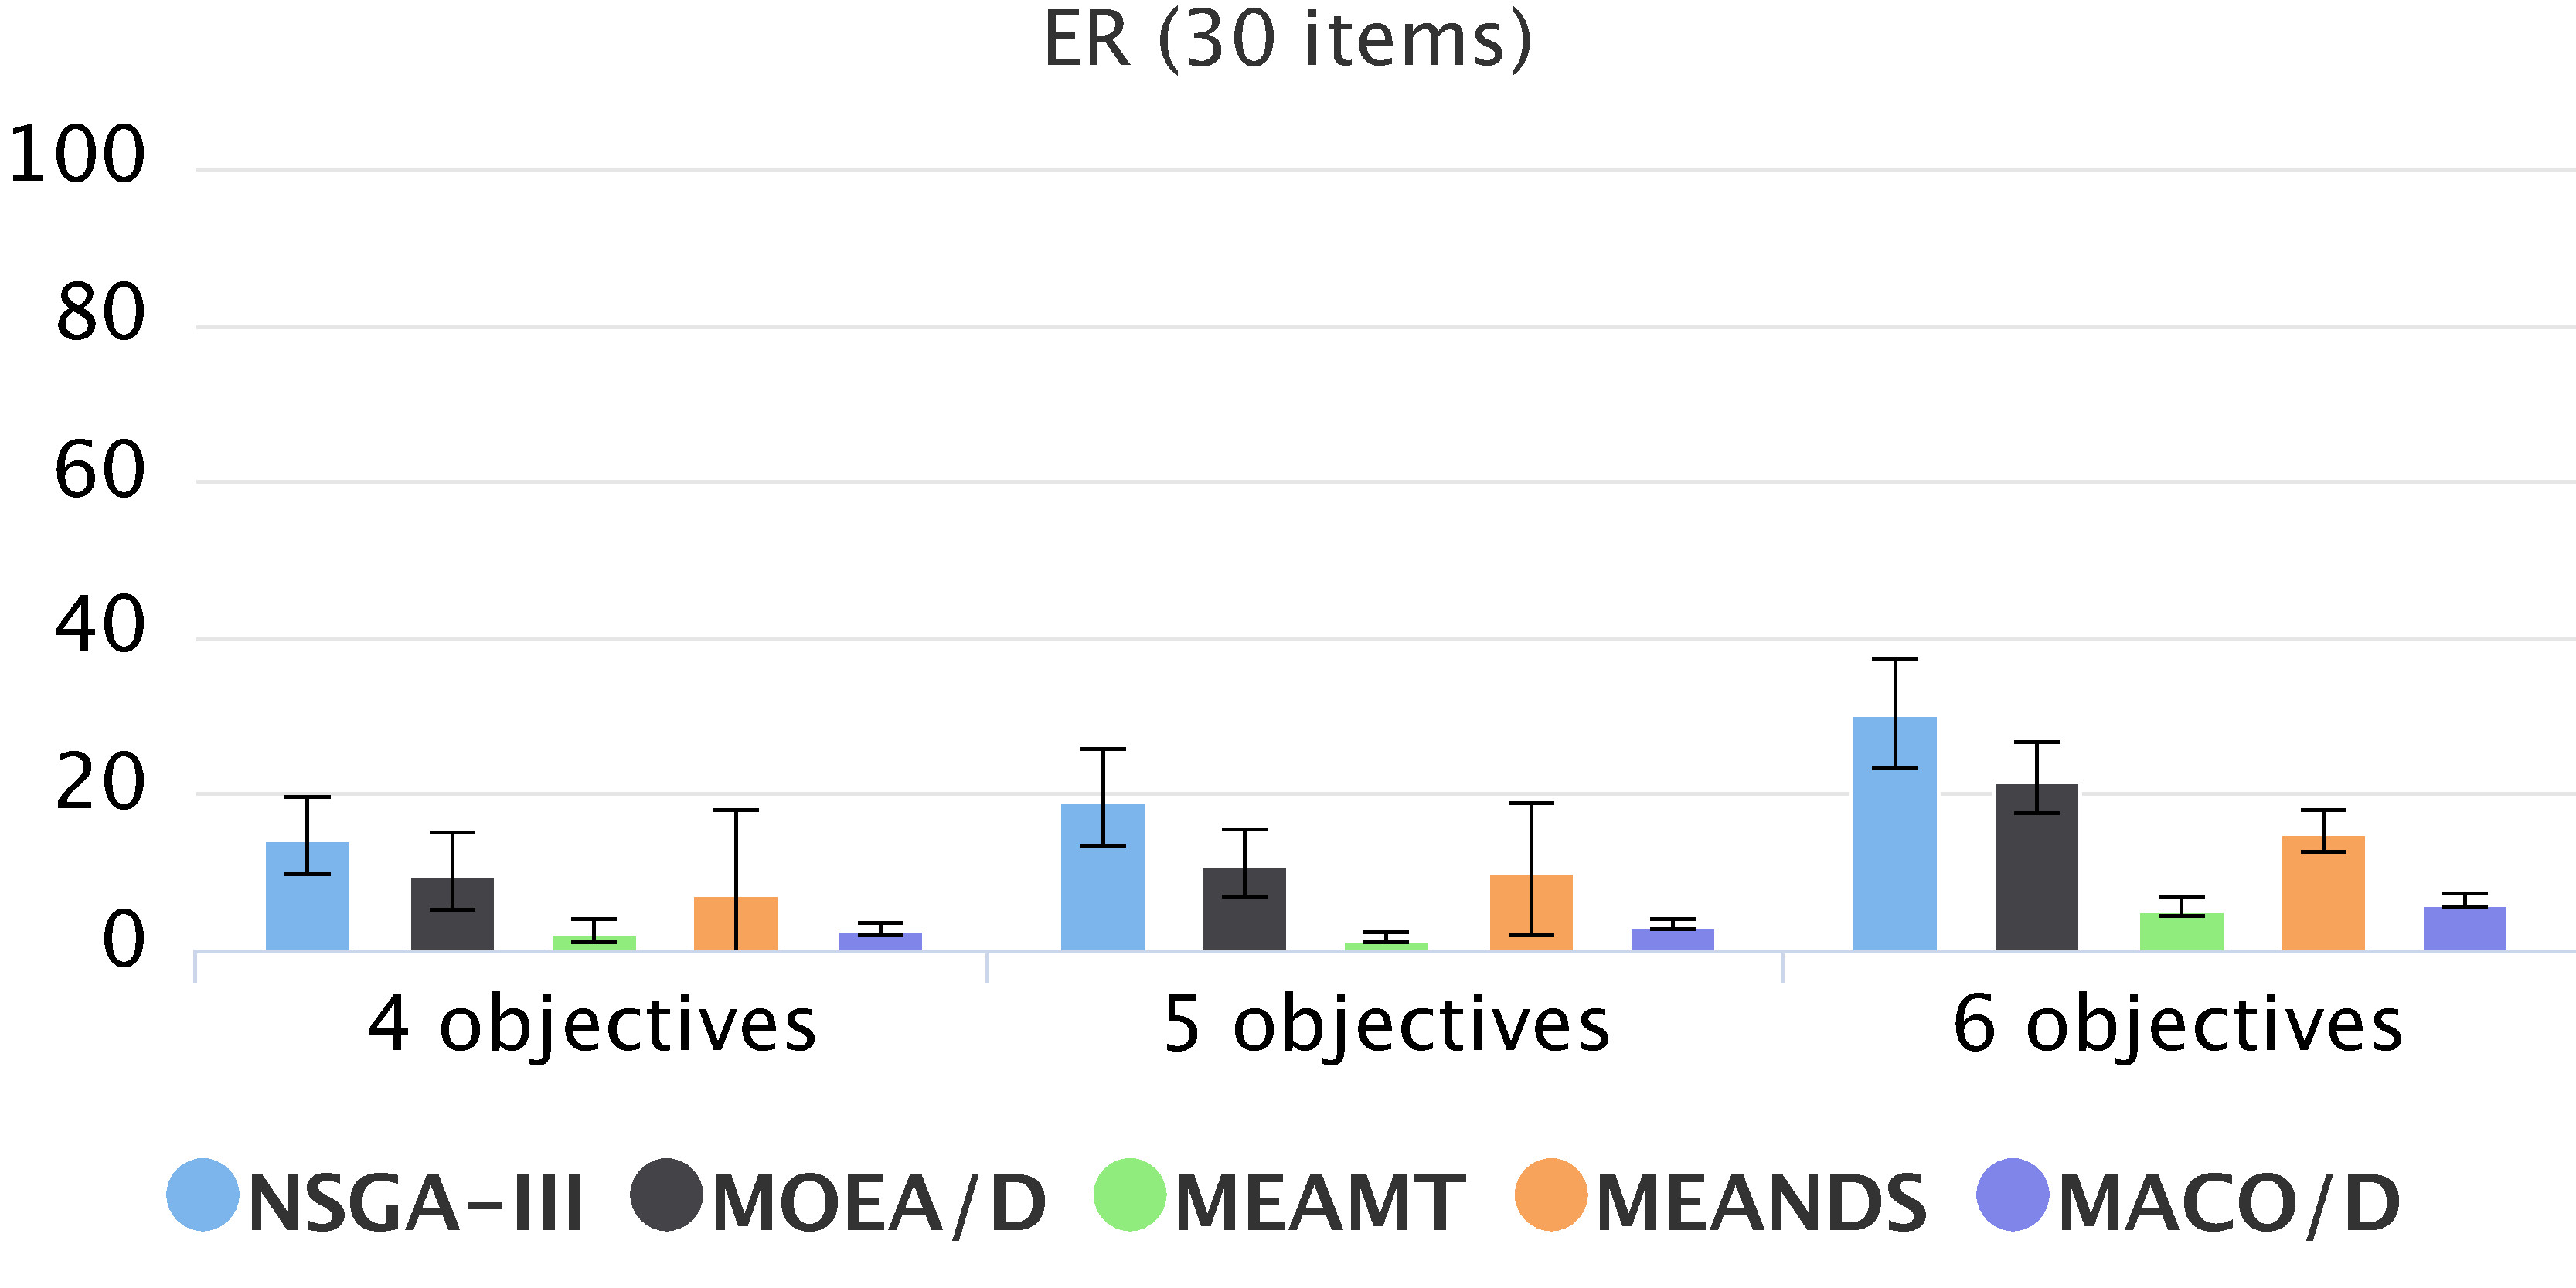
\includegraphics[width=0.5\textwidth]{cap_experimentos/figs/etapa3/er-mkp-30}
	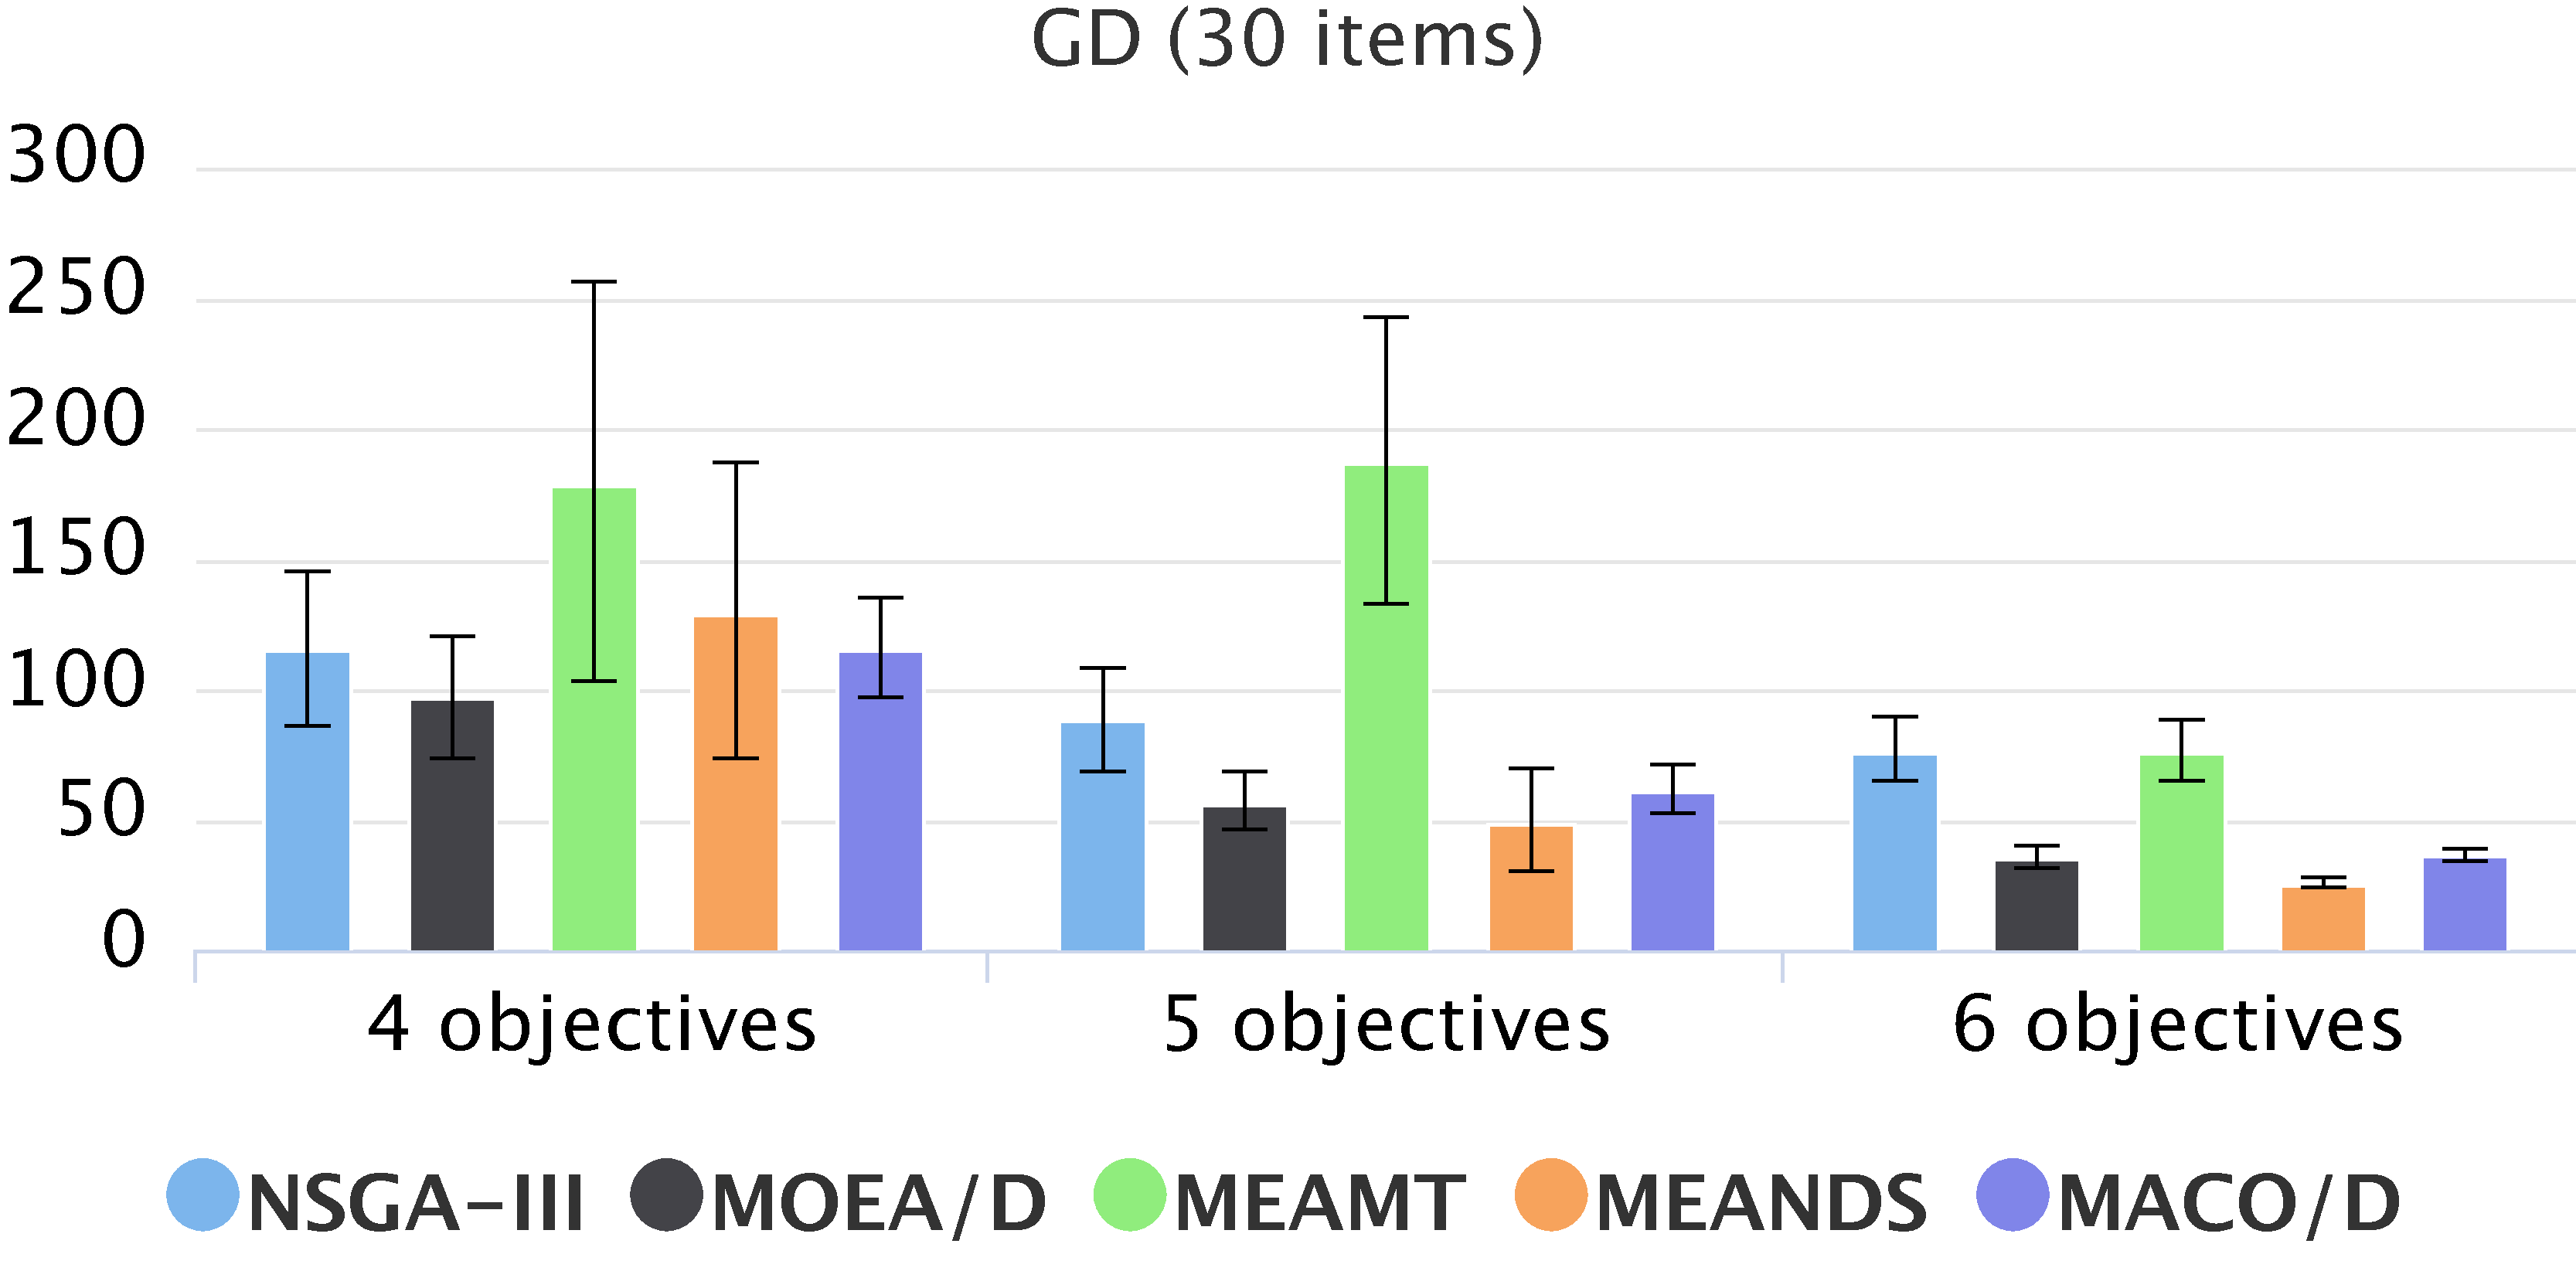
\includegraphics[width=0.5\textwidth]{cap_experimentos/figs/etapa3/gd-mkp-30}
	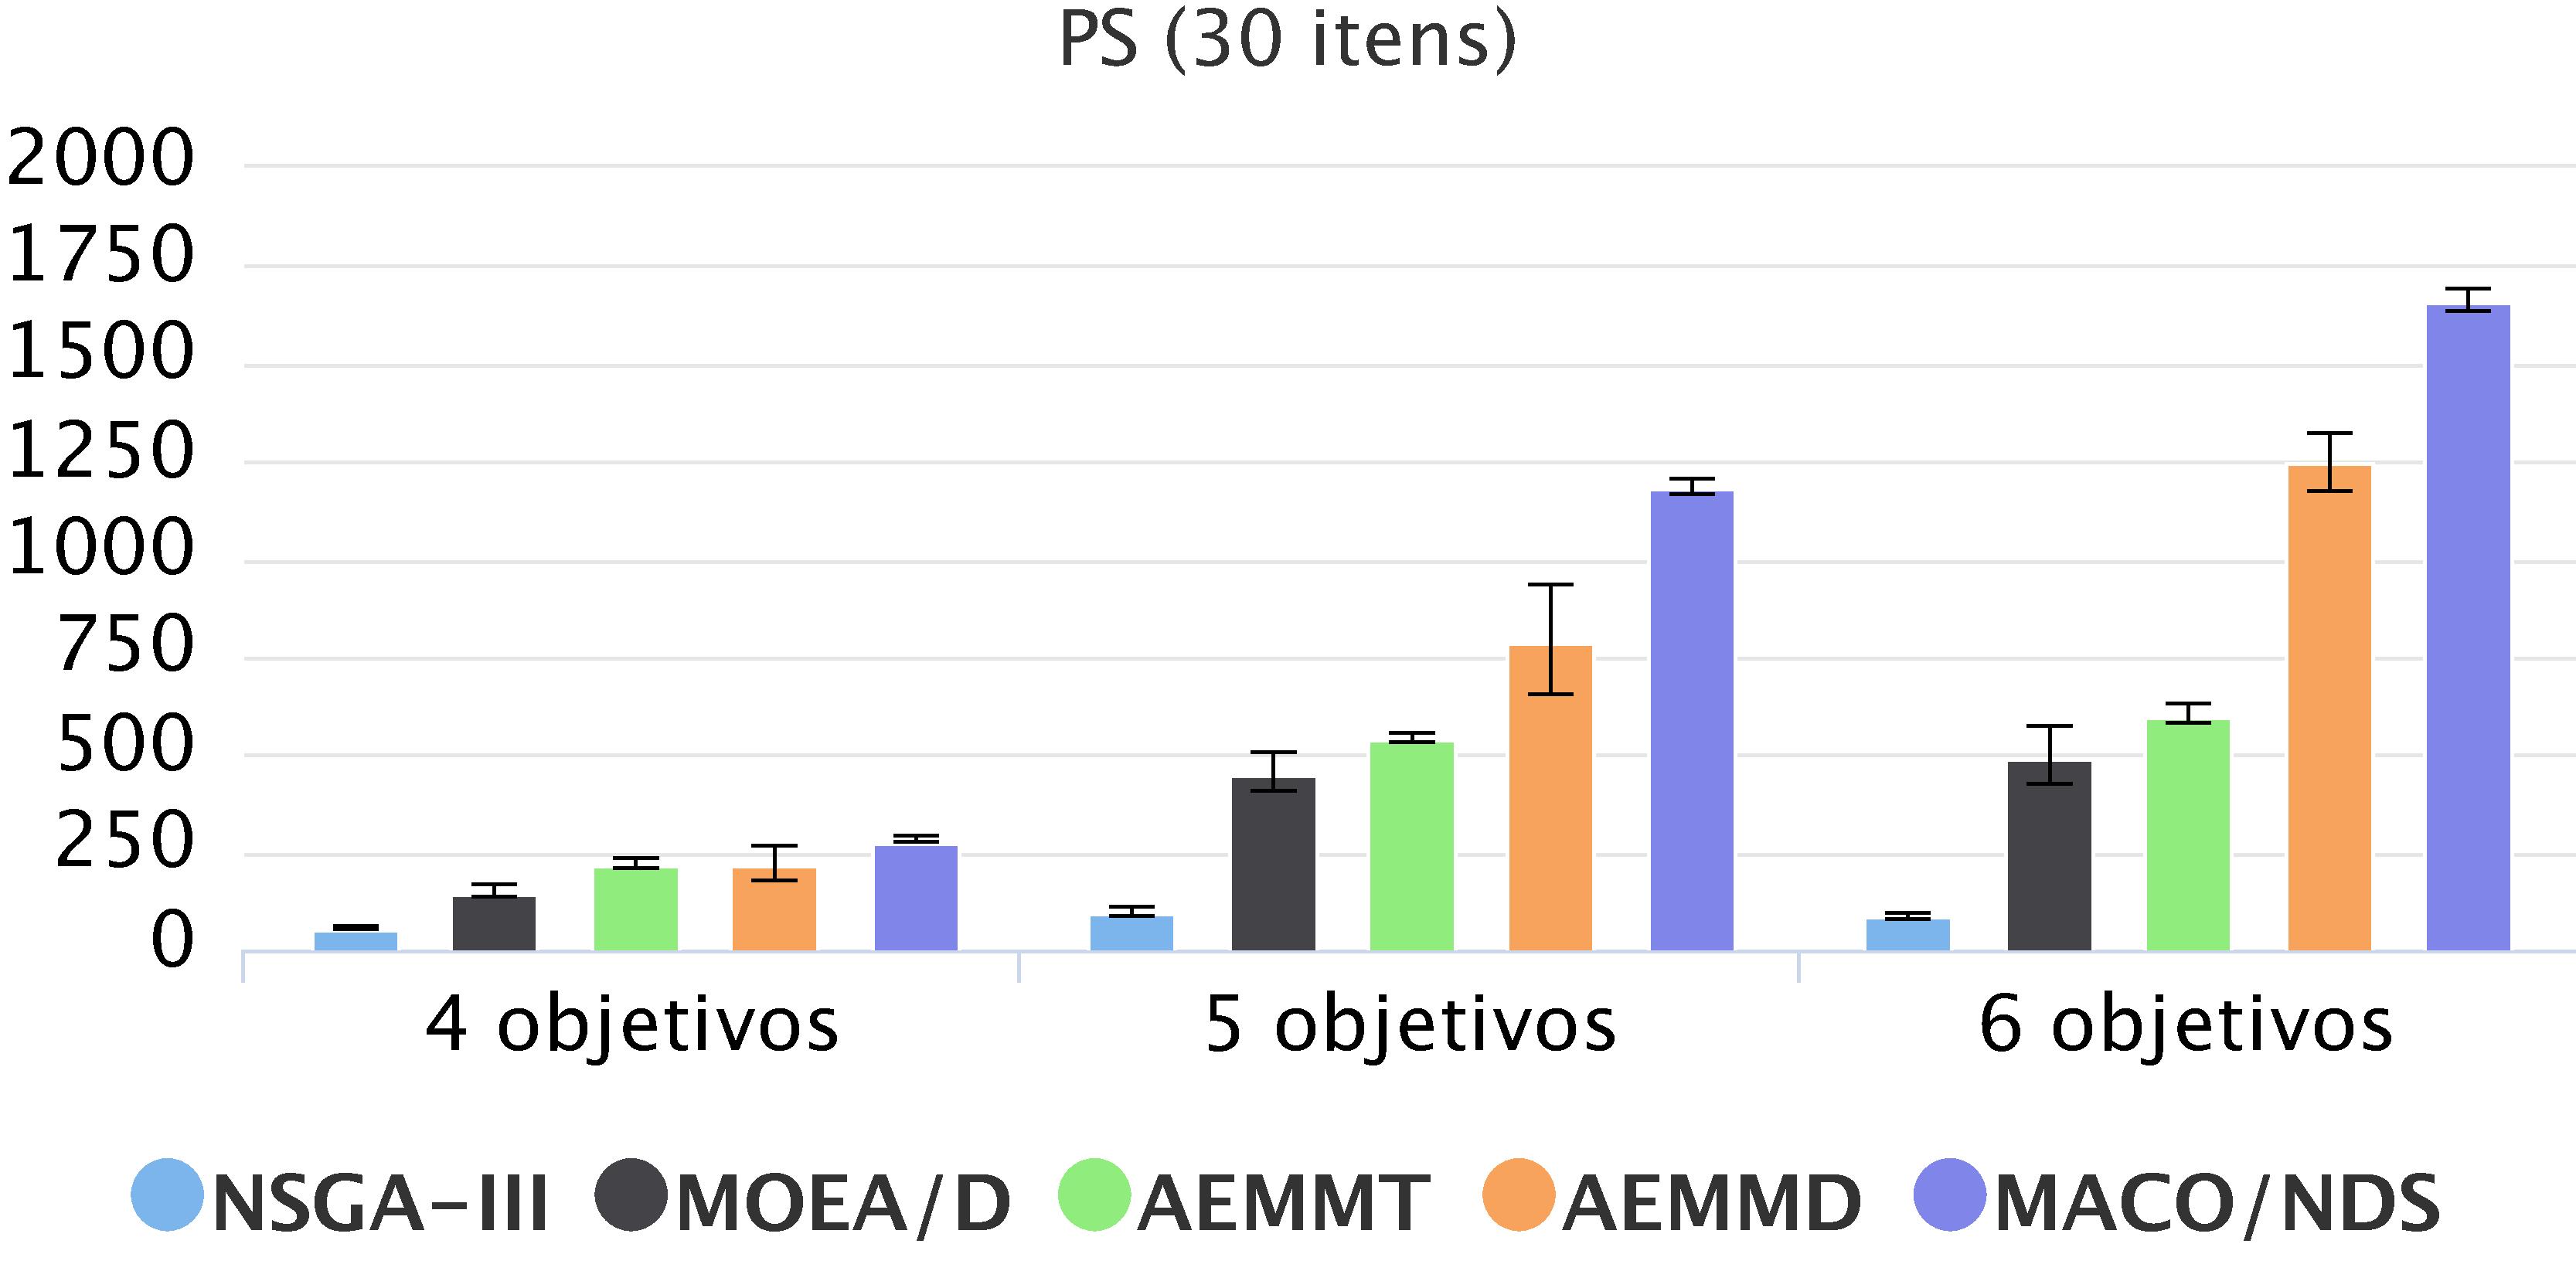
\includegraphics[width=0.5\textwidth]{cap_experimentos/figs/etapa3/ps-mkp-30}
	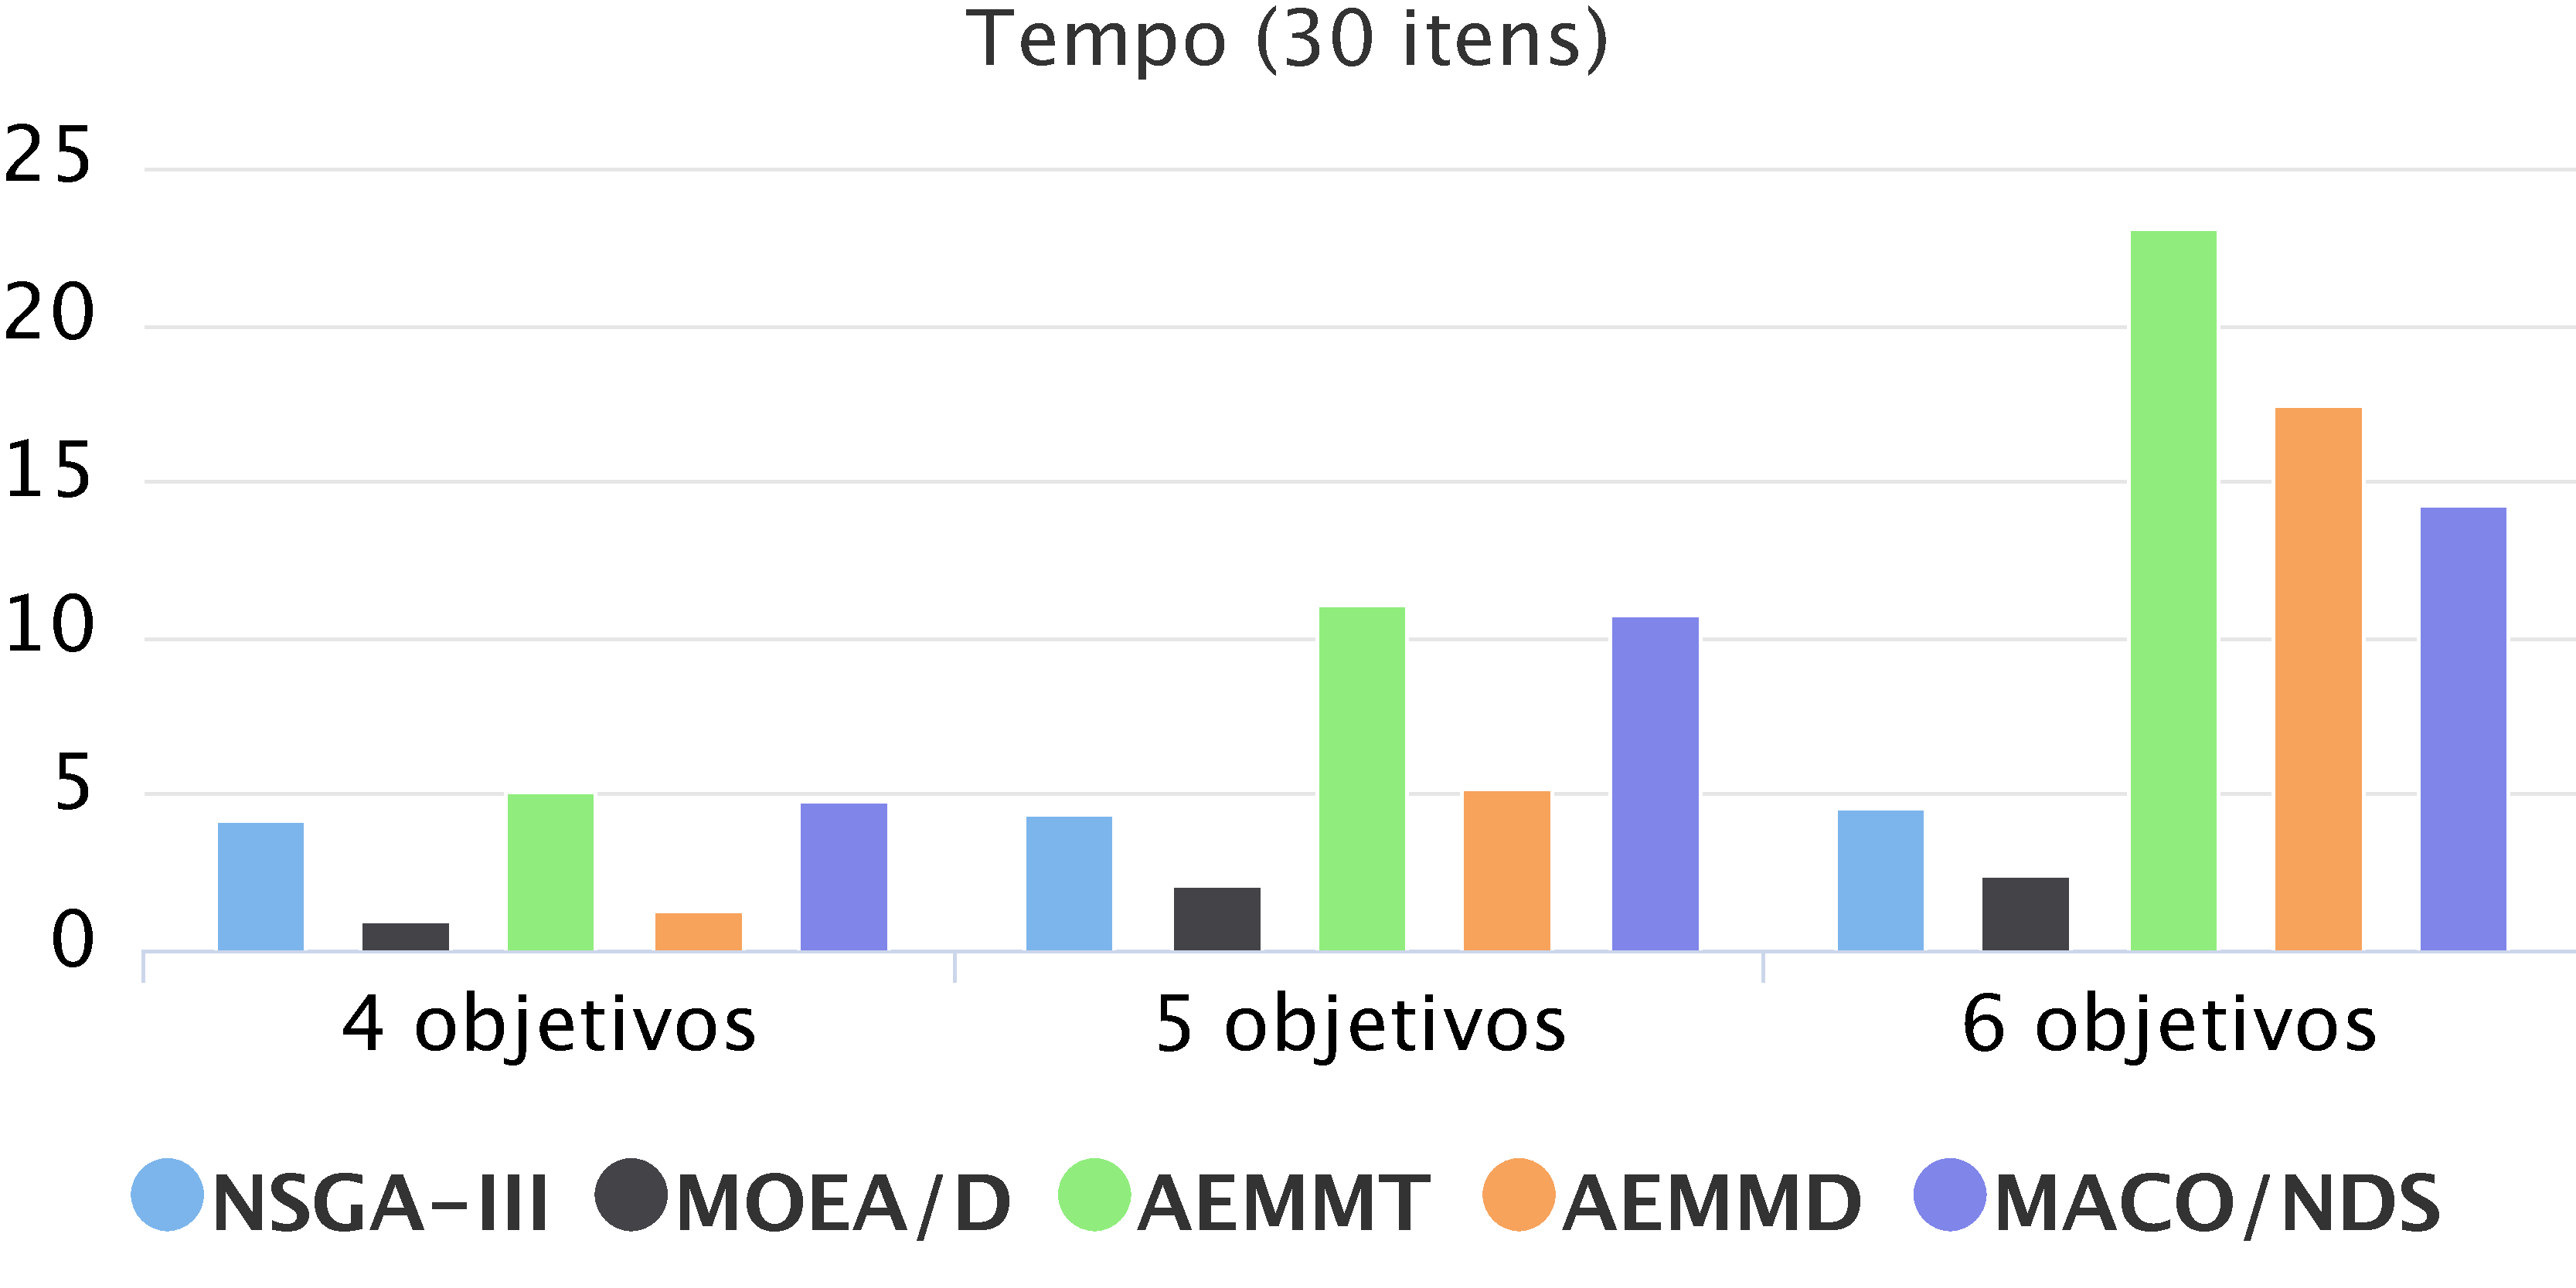
\includegraphics[width=0.5\textwidth]{cap_experimentos/figs/etapa3/time-mkp-30}
	\caption{\label{fig_exp3_pmm_30}Desempenho dos algoritmos na 3ª etapa para o PMM com 30 itens}
\end{figure*}

A \autoref{fig_exp3_pmm_30} retrata a versão mais simples do problema da mochila (30 itens). Nesse cenário, o AEMMT apresenta a menor taxa de erro dentre os algoritmos \textit{many-objective}, seguido pelo MACO/NDS e pelo AEMMD. Considerando a métrica GDp e a formulação com 4 objetivos, os melhores resultados são encontrados pelo MOEA/D, seguido pelo MACO/NDS. Com 5 e 6 objetivos, o AEMMD produz o menor $GD$, sendo acompanhado de perto pelo MACO/NDS. Na métrica $PS$, o MACO/NDS é o algoritmo com melhor desempenho para todas as formulações de objetivo. Na sequência, os algoritmos com os melhores valores de $PS$ são: AEMMD, AEMMT, MOEA/D e NSGA-III. Destre esses algoritmos, o único com um limite fixo no tamanho do Pareto é o NSGA-III. Portanto, é esperado que possua um valor de $PS$ menor. Quanto ao tempo, o MOEA/D é o algoritmo mais rápido, enquanto que o AEMMT é o mais lento. No geral, o MACO/NDS apresentou o melhor equilíbrio entre as métricas de desempenho, revelando-se a melhor opção, nessa instância (30 itens), para formulações com muitos objetivos. Além disso, o MACO/NDS apresenta os menores desvios padrões, ou seja, é o método com maior estabilidade quanto à qualidade de suas soluções, independentemente da execução.

\begin{figure*}[!htbp]	
	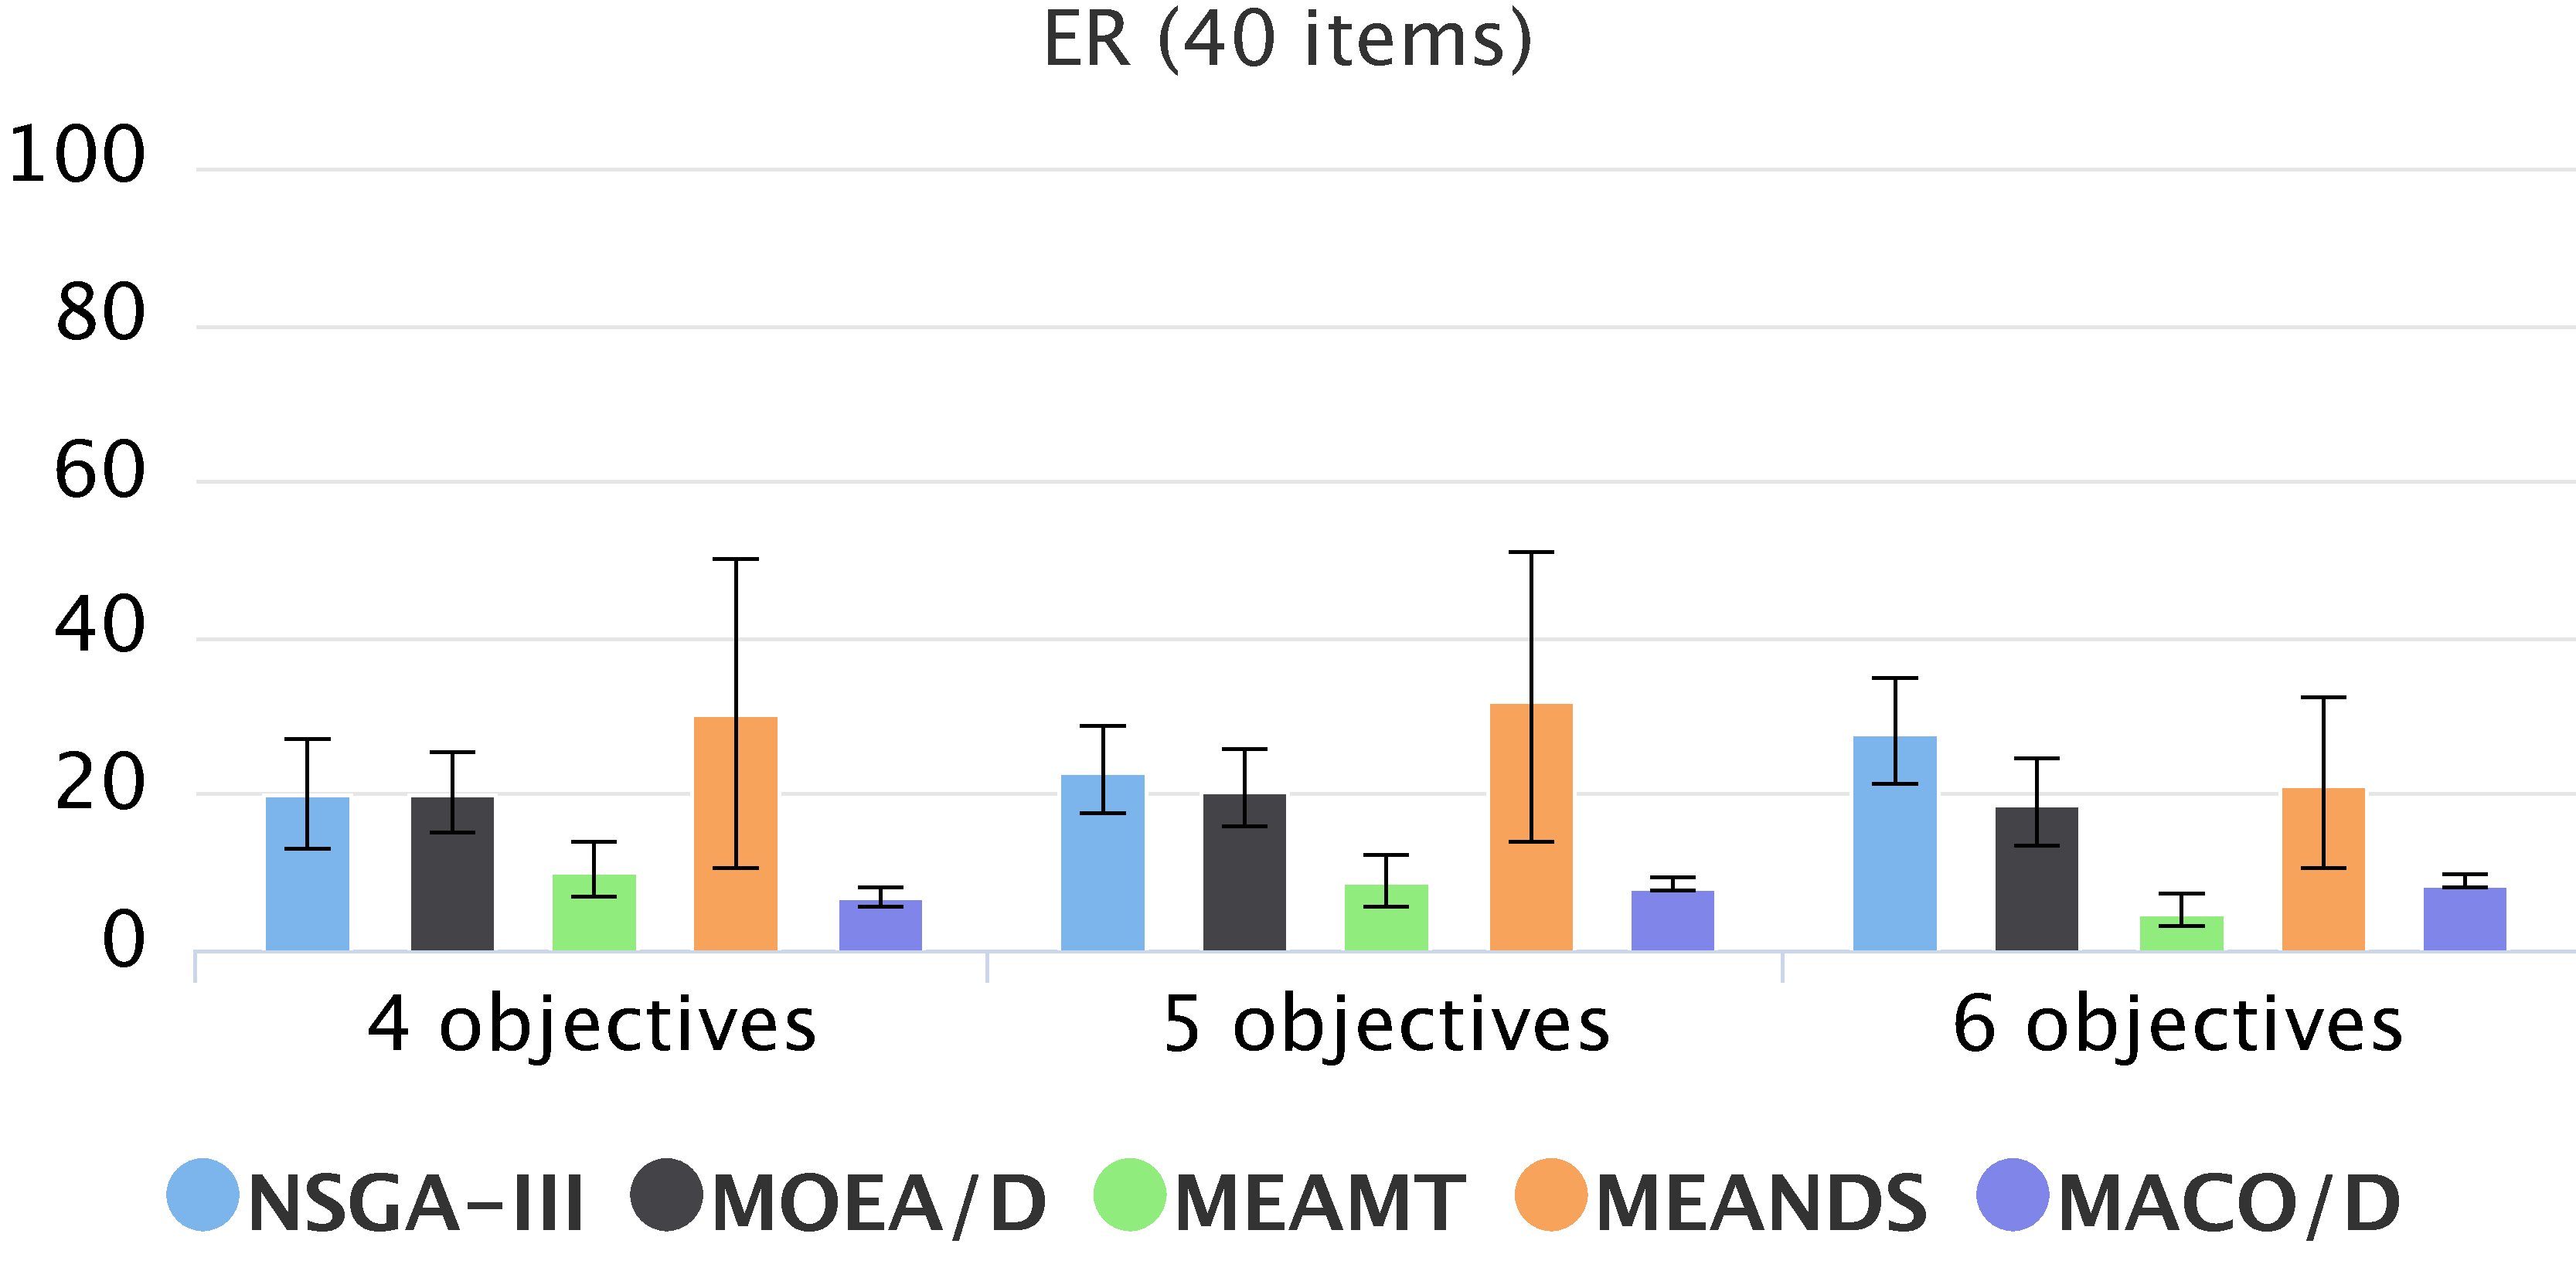
\includegraphics[width=0.5\textwidth]{cap_experimentos/figs/etapa3/er-mkp-40}
	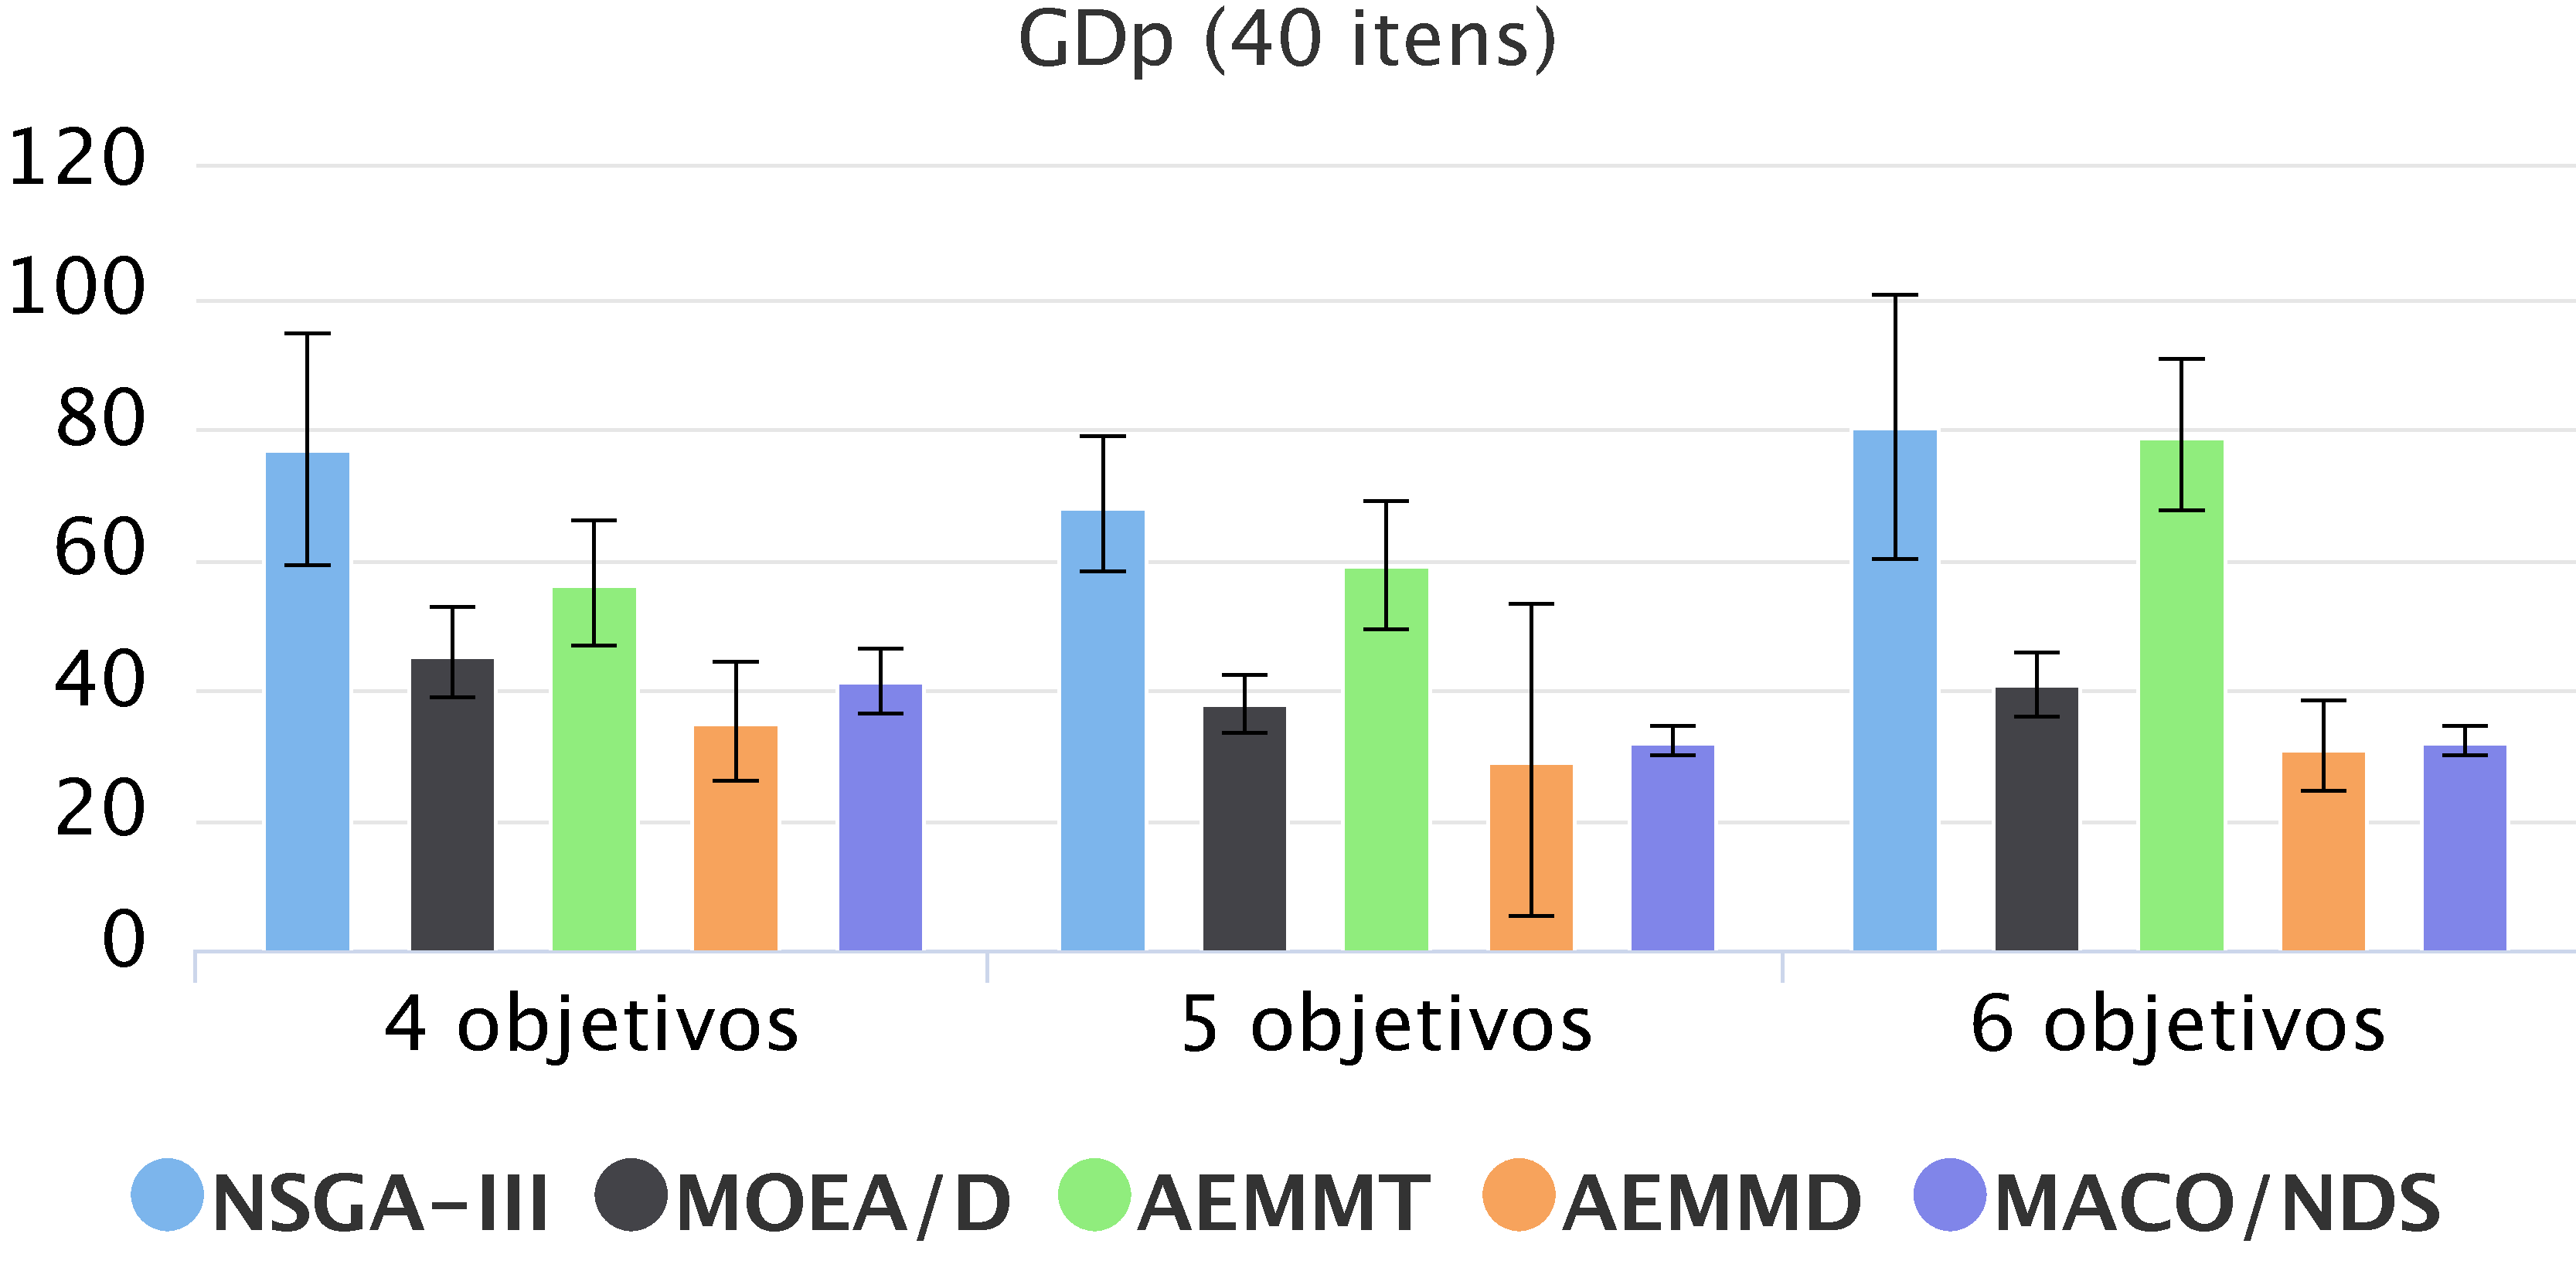
\includegraphics[width=0.5\textwidth]{cap_experimentos/figs/etapa3/gd-mkp-40}
	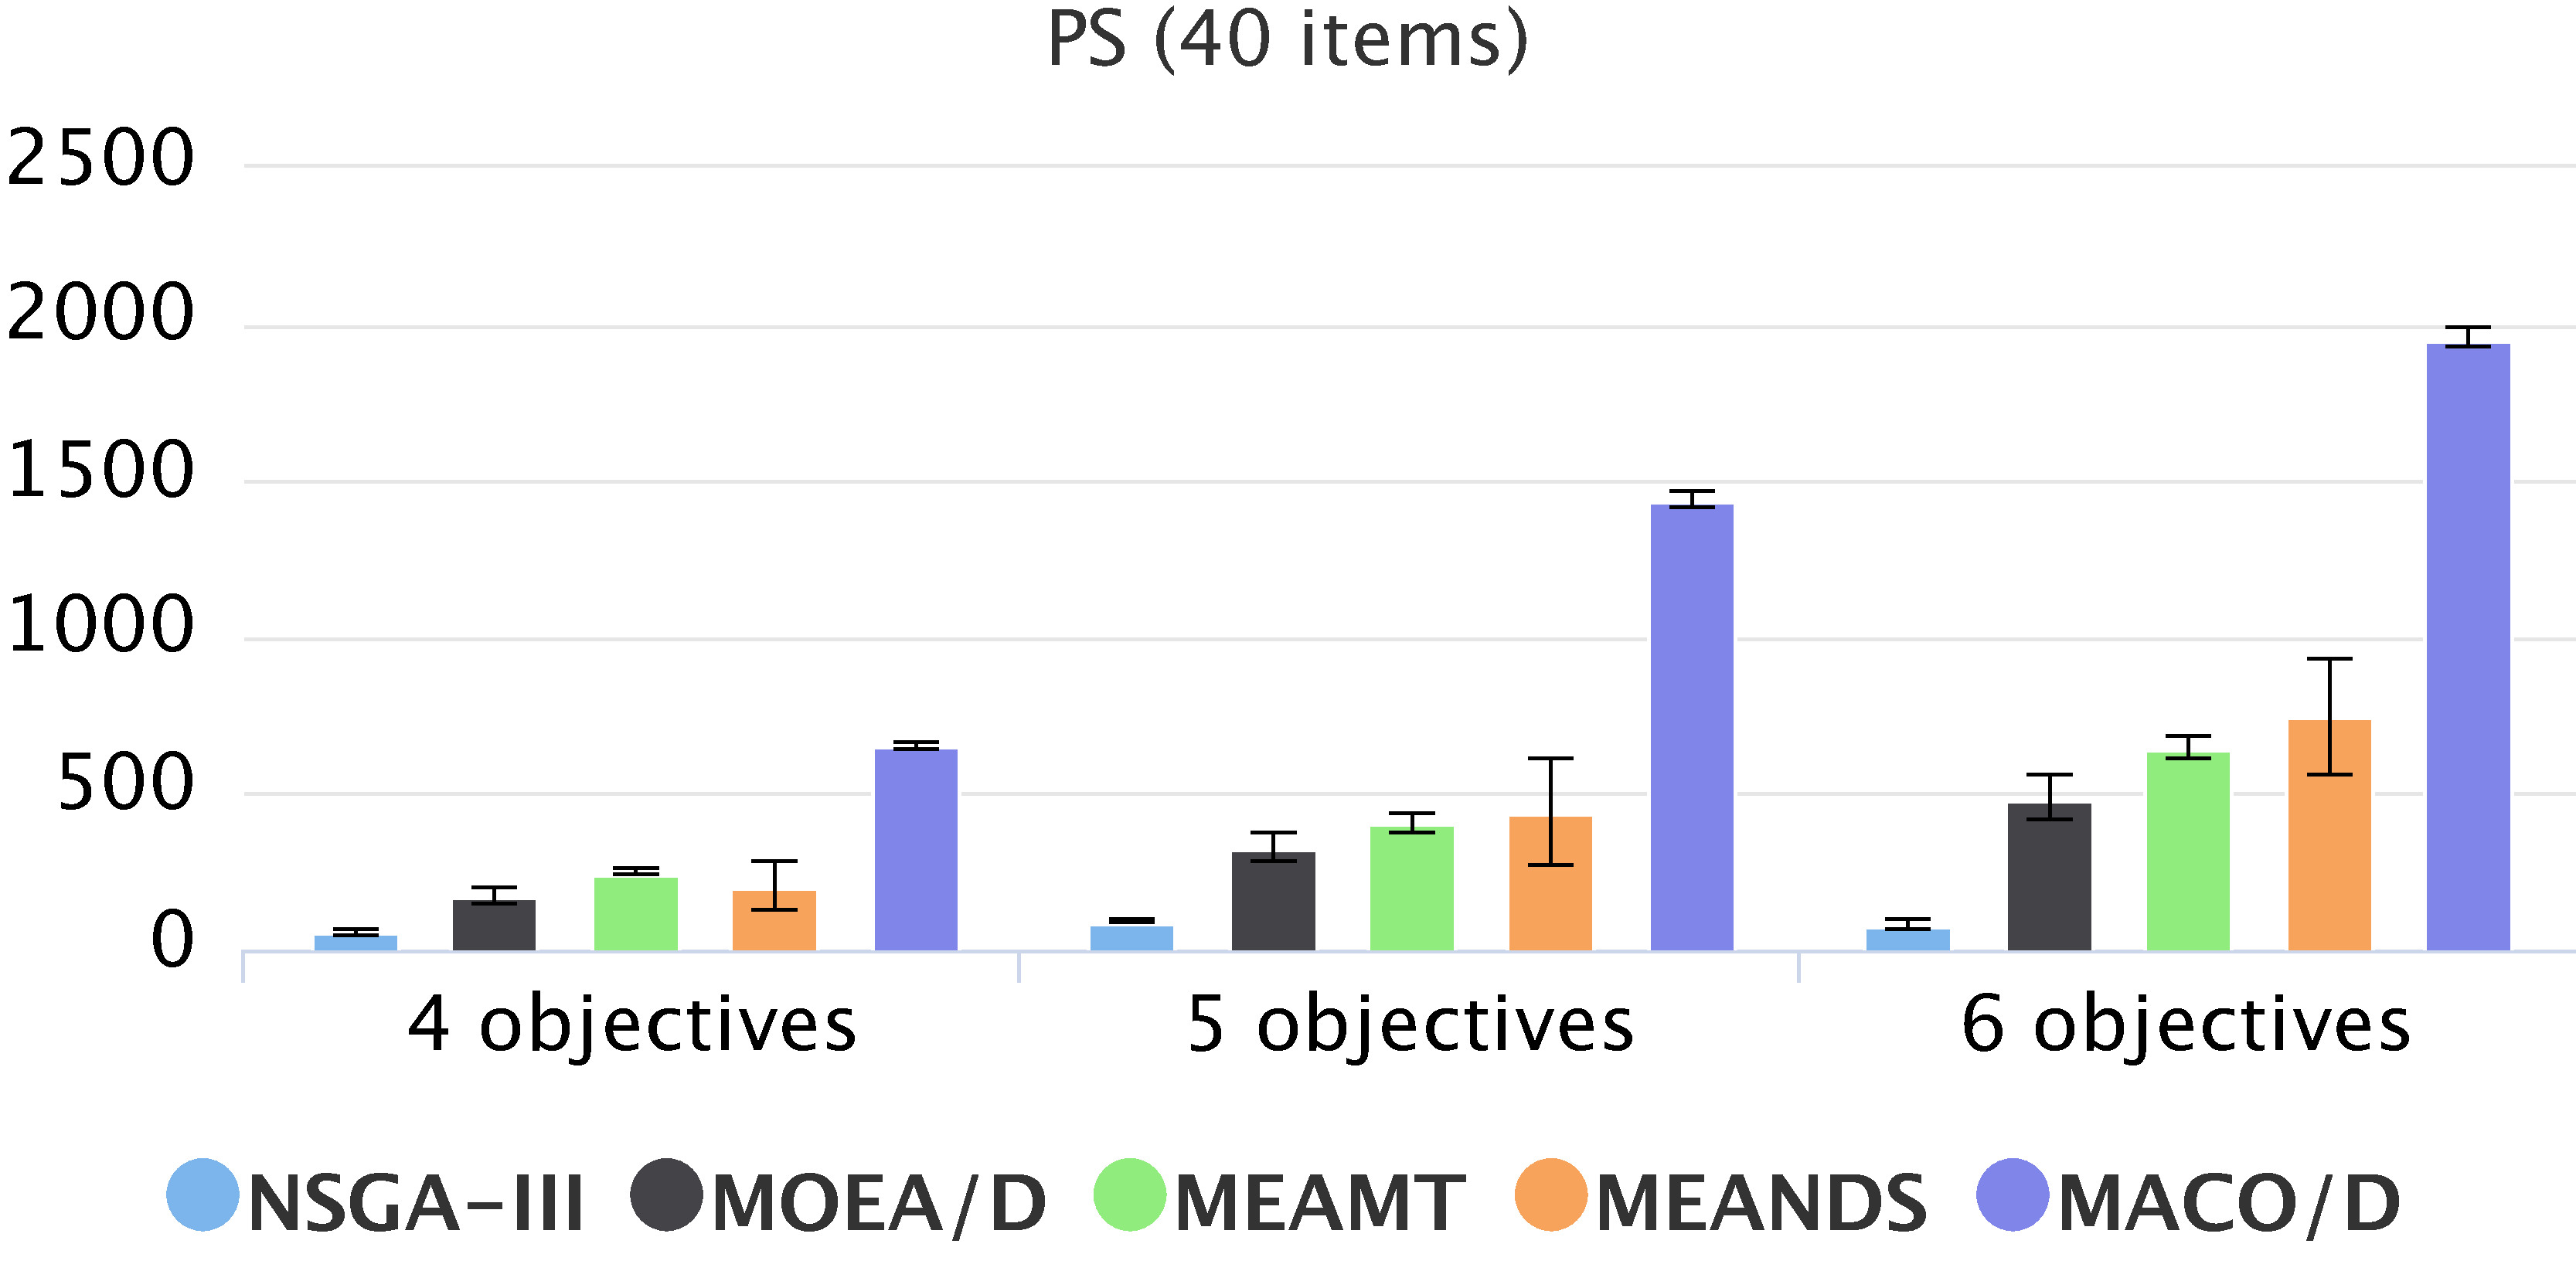
\includegraphics[width=0.5\textwidth]{cap_experimentos/figs/etapa3/ps-mkp-40}
	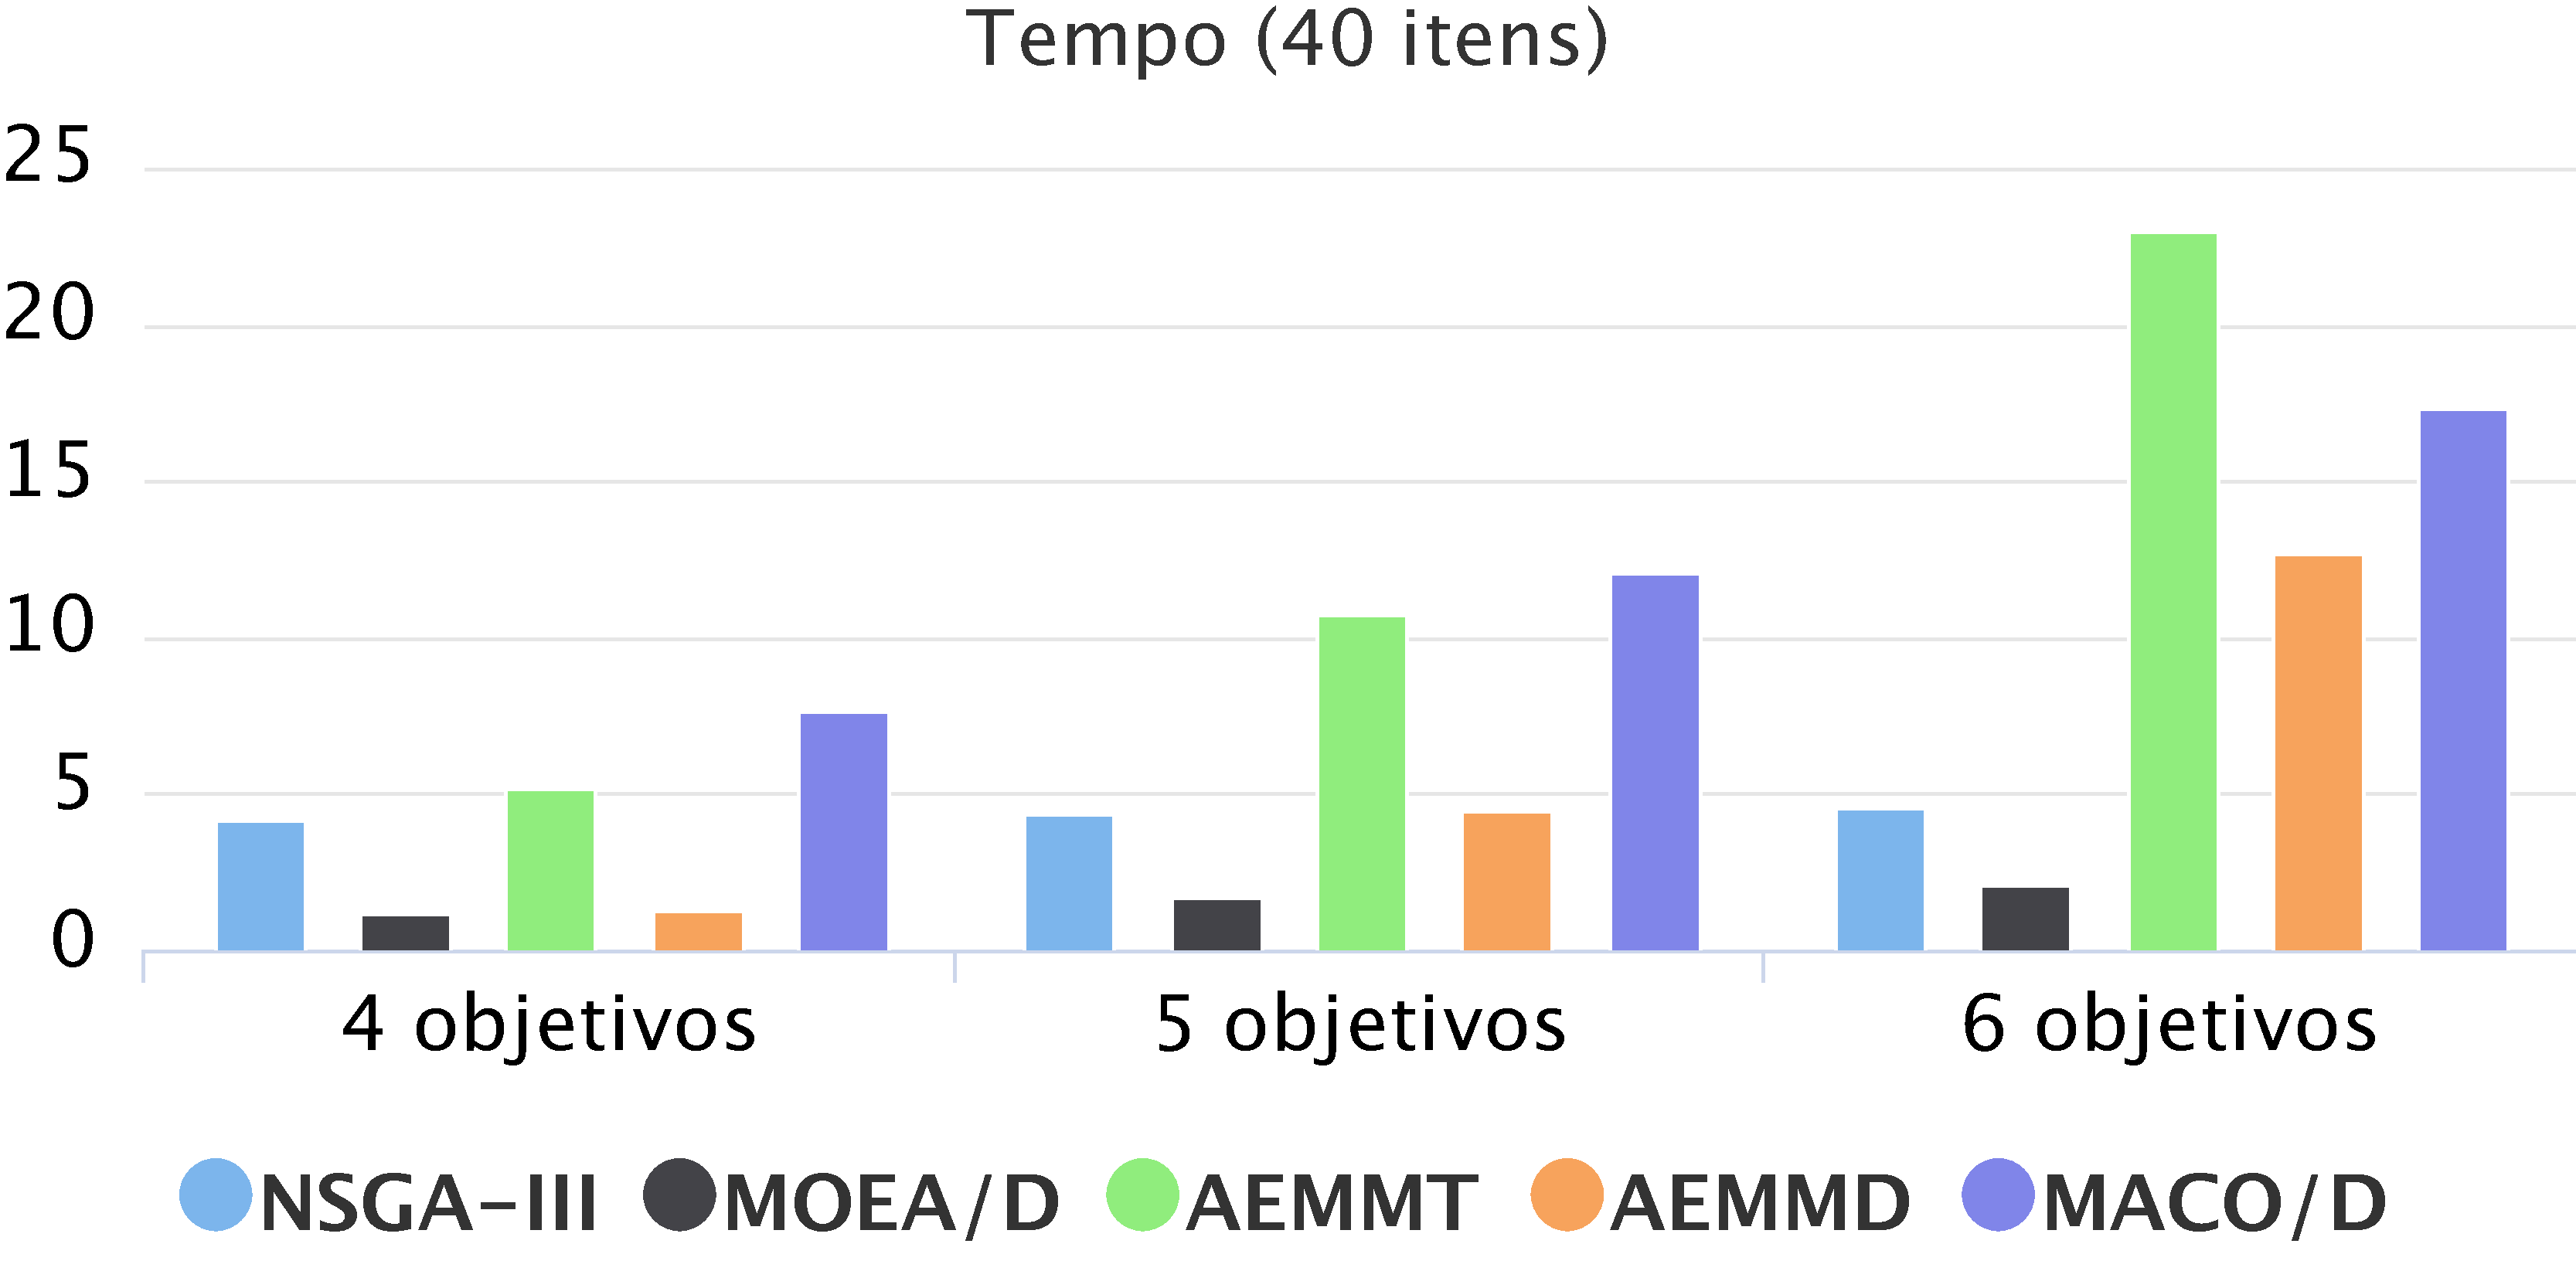
\includegraphics[width=0.5\textwidth]{cap_experimentos/figs/etapa3/time-mkp-40}
	\caption{\label{fig_exp3_pmm_40}Desempenho dos algoritmos na 3ª etapa para o PMM com 40 itens}
\end{figure*}

Os resultados obtidos para o PMM de 40 itens é apresentado na \autoref{fig_exp3_pmm_40}. O AEMMT e o MACO/NDS apresentam as menores taxas de erro, sendo que o MACO/NDS é melhor para 4 e 5 objetivos (6,9\% e 8,4\%, respectivamente), enquanto o AEMMT obtém o melhor resultado para 6 objetivos (5,1\% contra 8,7\% do MACO/NDS). Os melhores valores de $GDp$ foram encontrados pelo AEMMD e MACO/NDS, sendo o primeiro um pouco melhor que o segundo. Em contrapartida, o AEMMD apresenta uma alta variação nos resultados, indicando que algumas execuções produzem soluções muito próximas do Pareto enquanto outras nem tanto. Considerando o tamanho dos Paretos encontrados ($PS$), novamente o MACO/NDS retorna os melhores valores independentemente da formulação de objetivos. Em termos do tempo médio de execução, o MOEA/D é o algoritmo mais rápido (5,2 segundos ao somar o tempo das 3 formulações de objetivos), enquanto o AEMMT e o MACO/NDS são os mais lentos (39 e 37,2 segundos, ao somar o tempo das 3 formulações de objetivos, respectivamente).

\begin{figure*}[!htbp]
	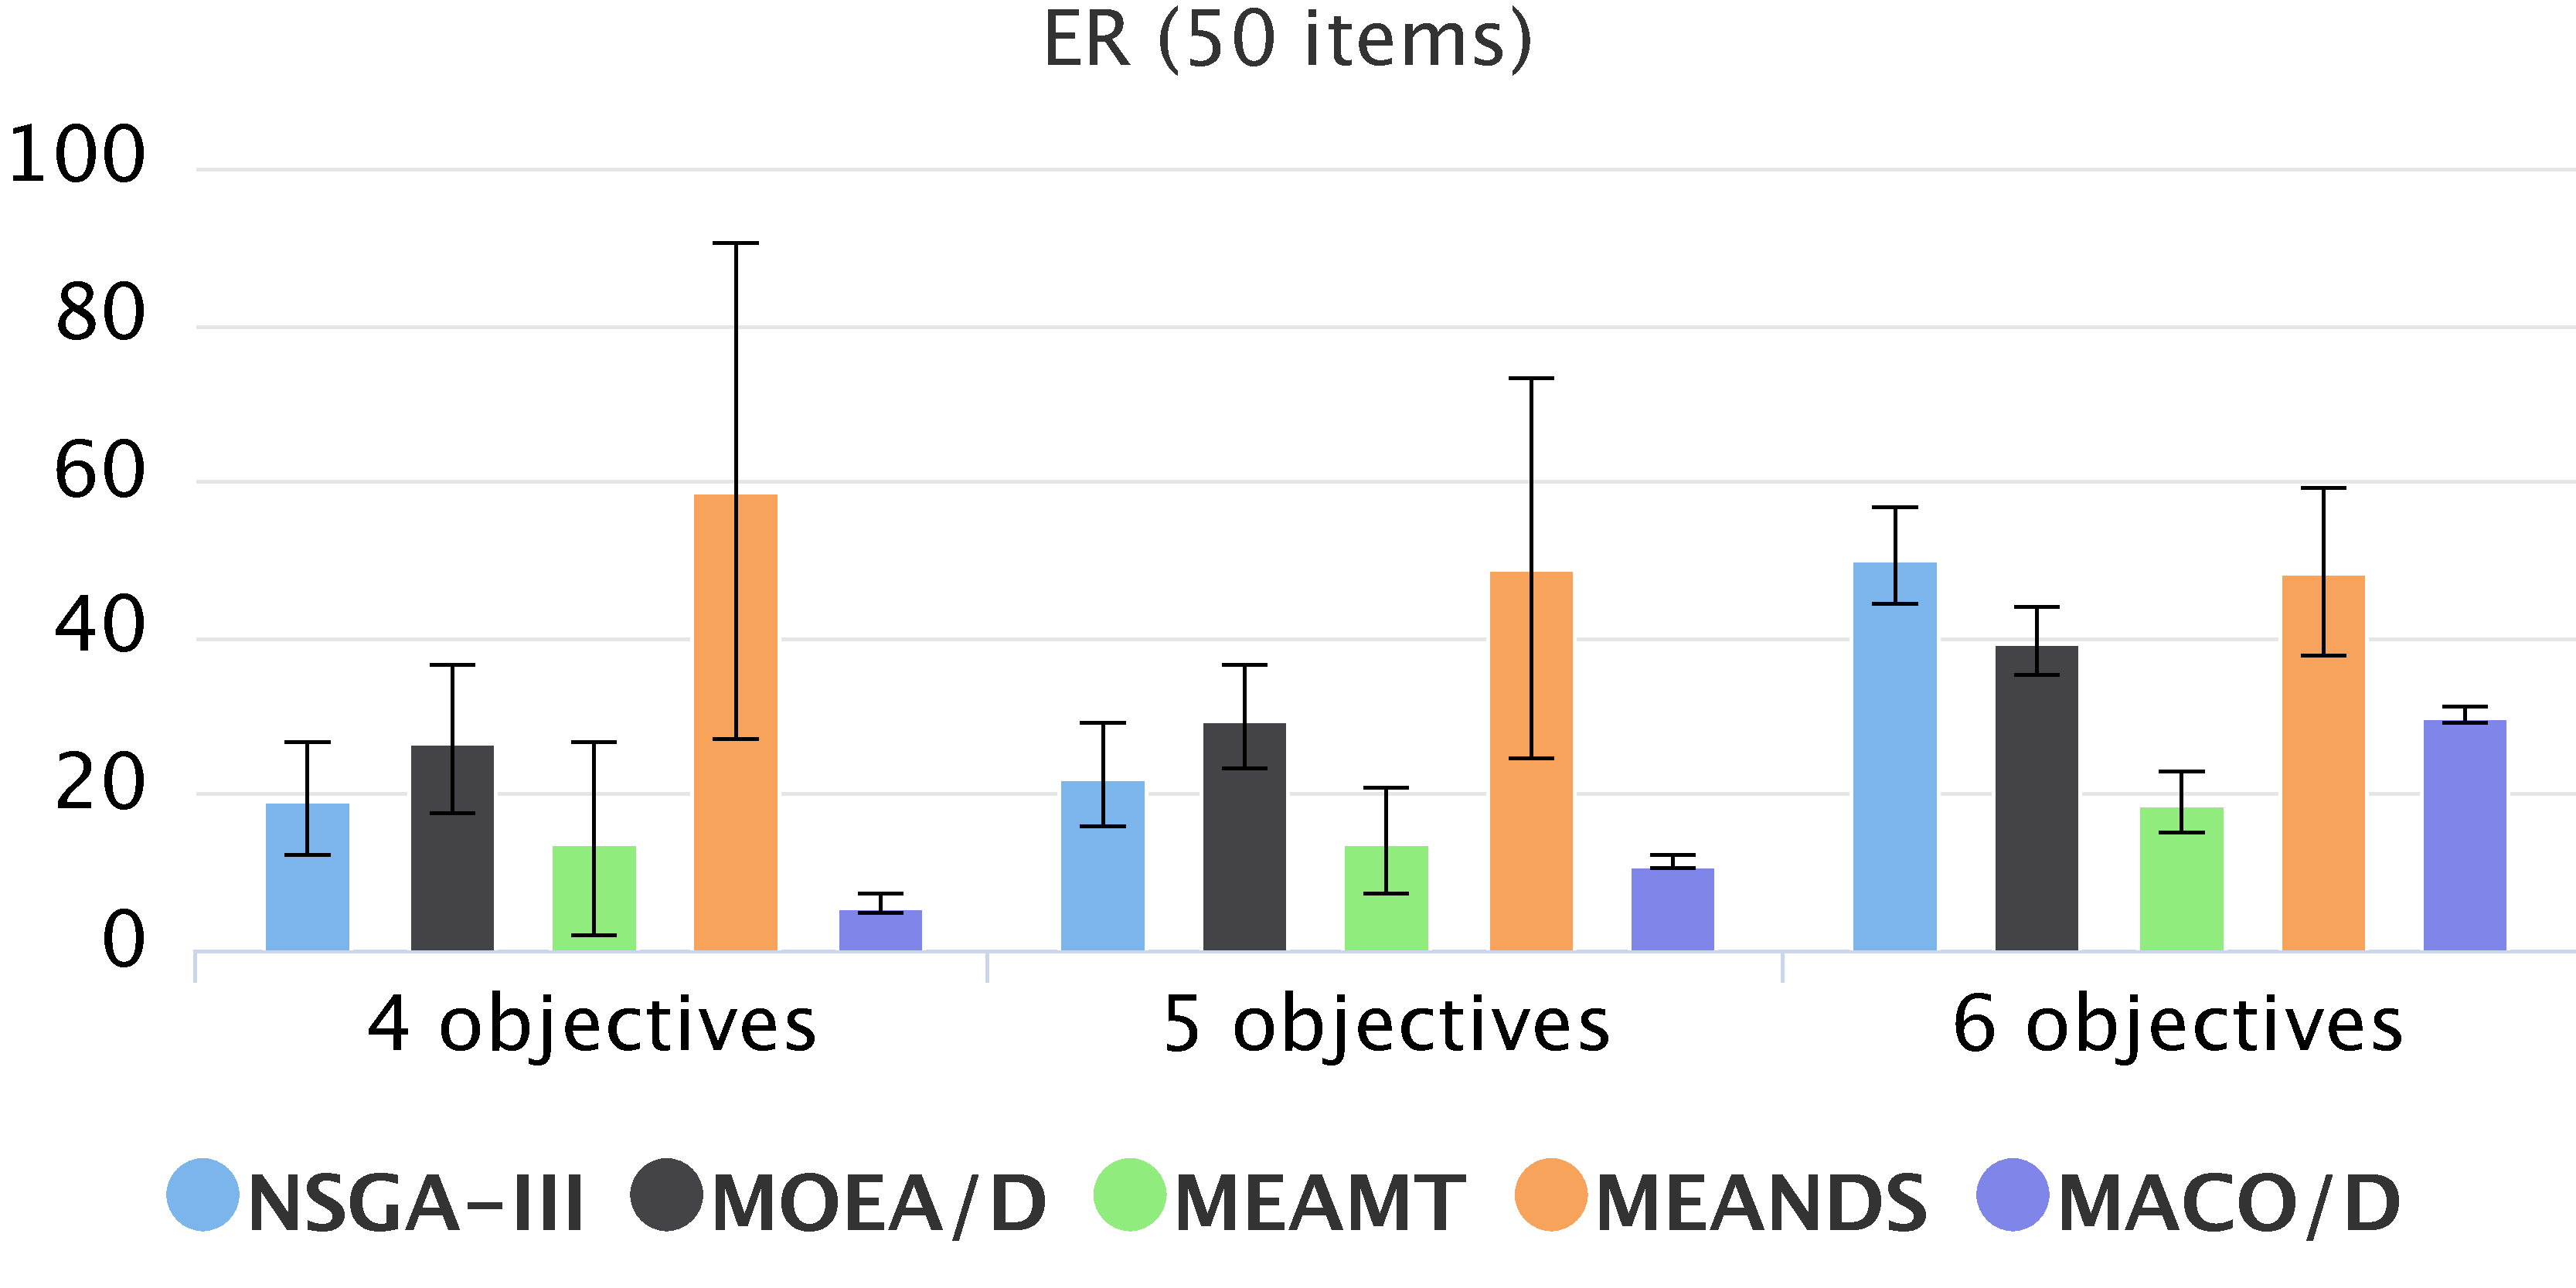
\includegraphics[width=0.5\textwidth]{cap_experimentos/figs/etapa3/er-mkp-50}
	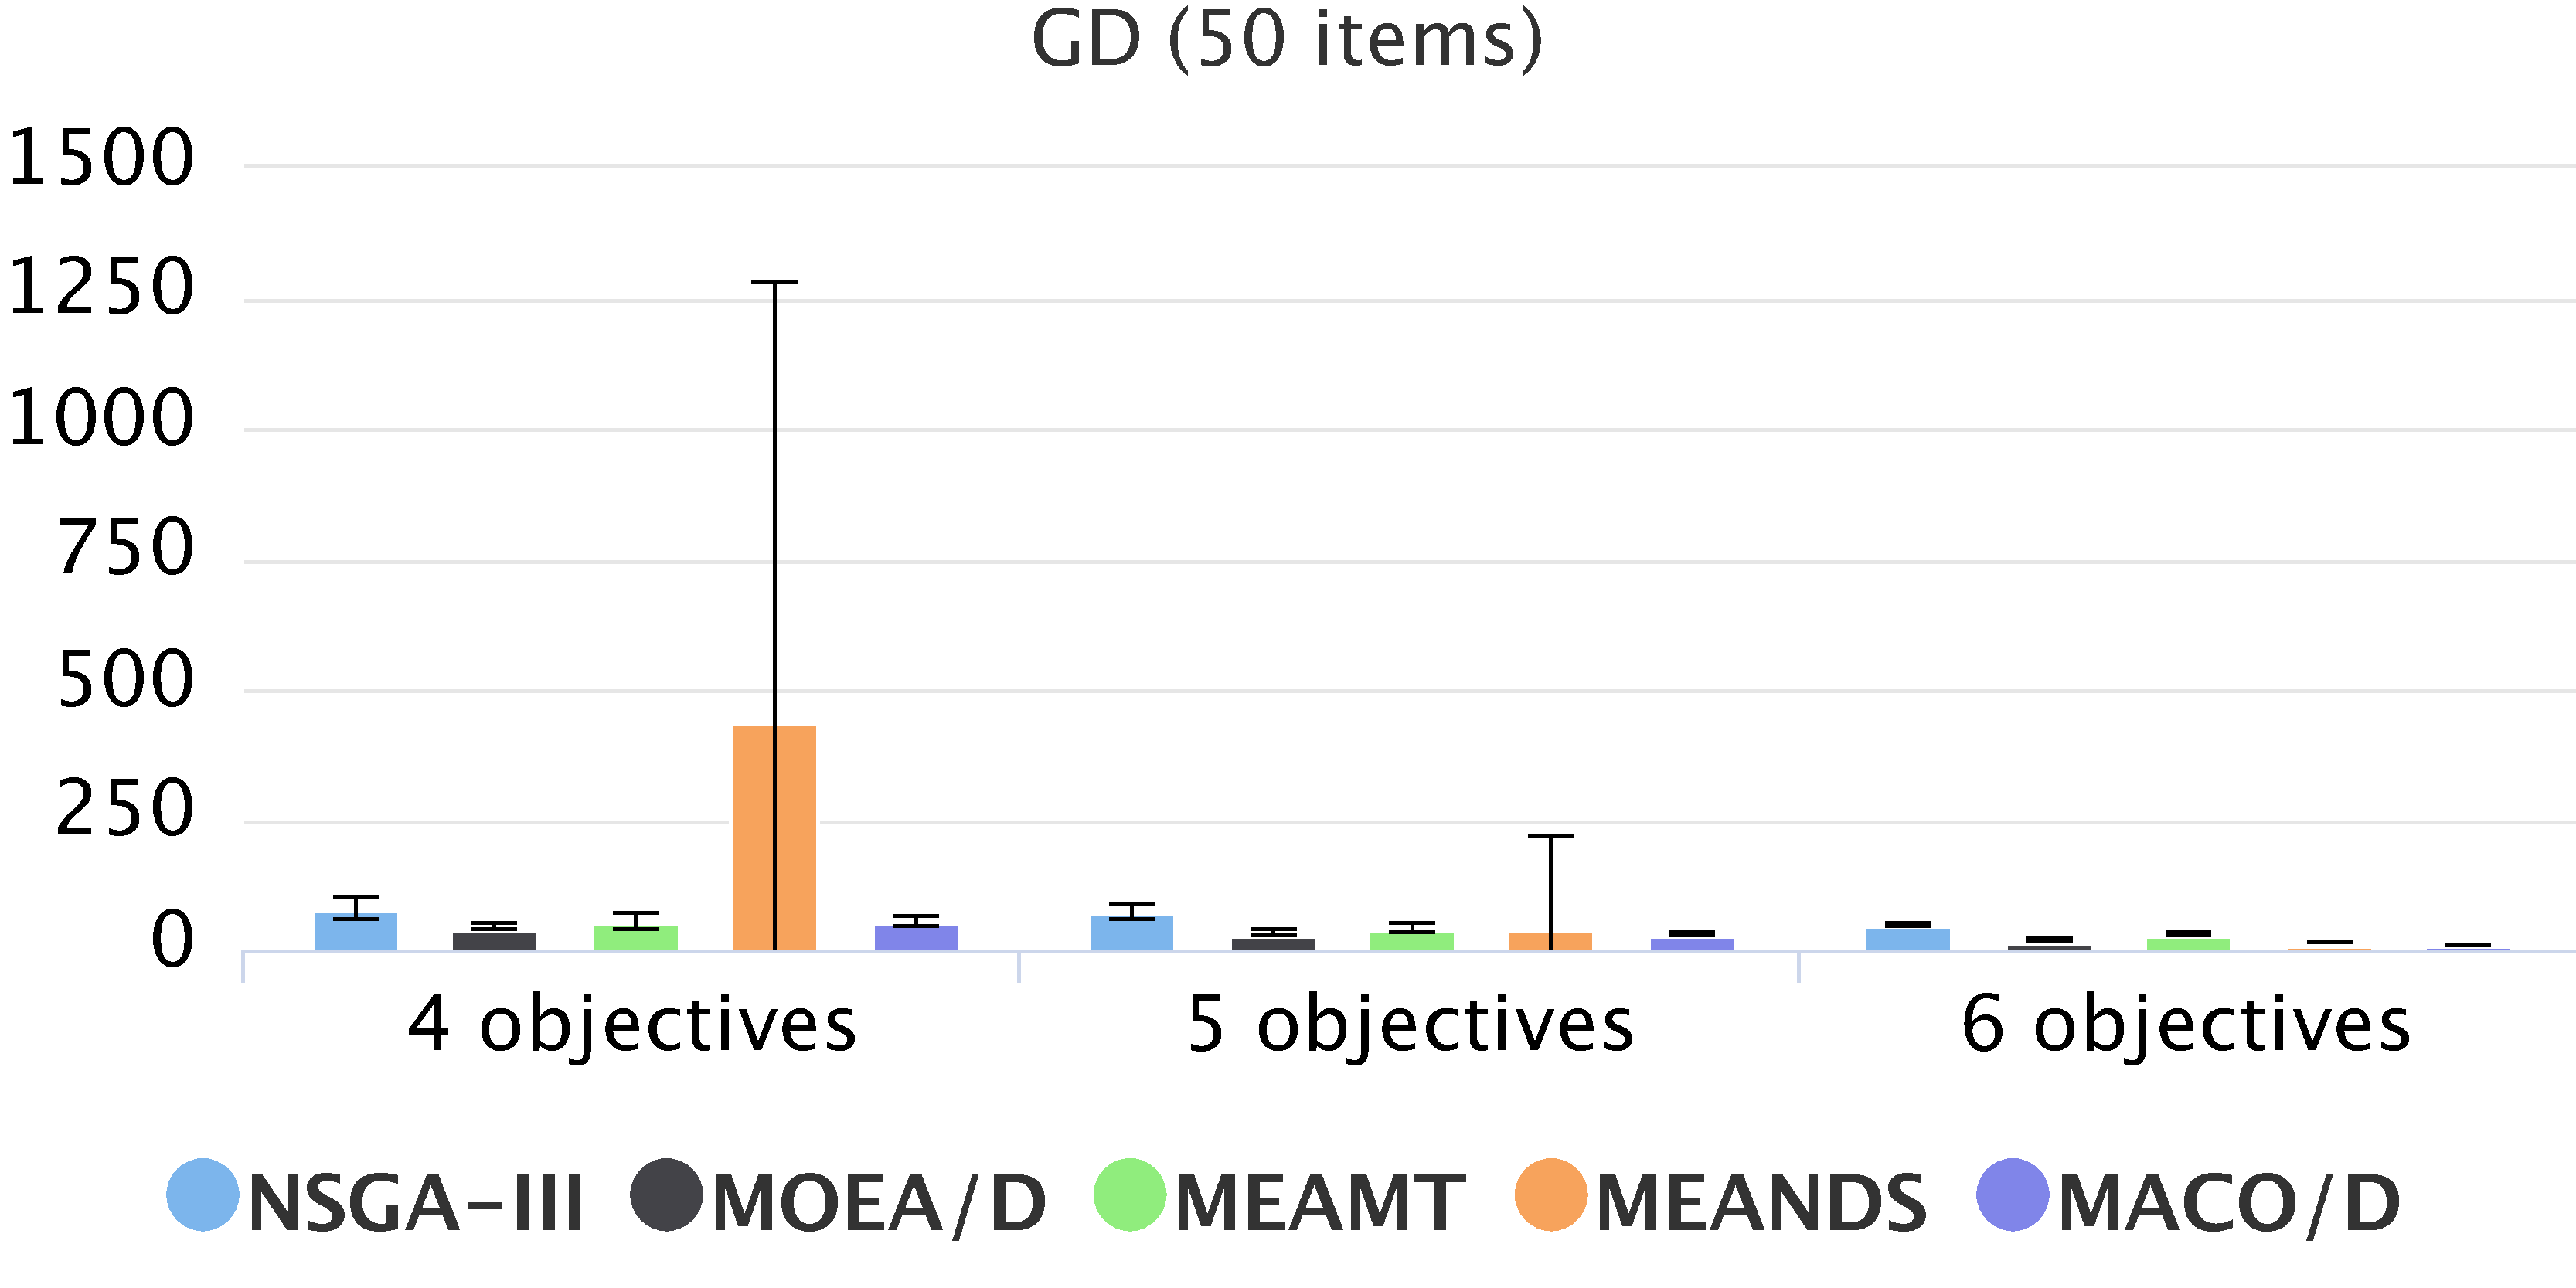
\includegraphics[width=0.5\textwidth]{cap_experimentos/figs/etapa3/gd-mkp-50}
	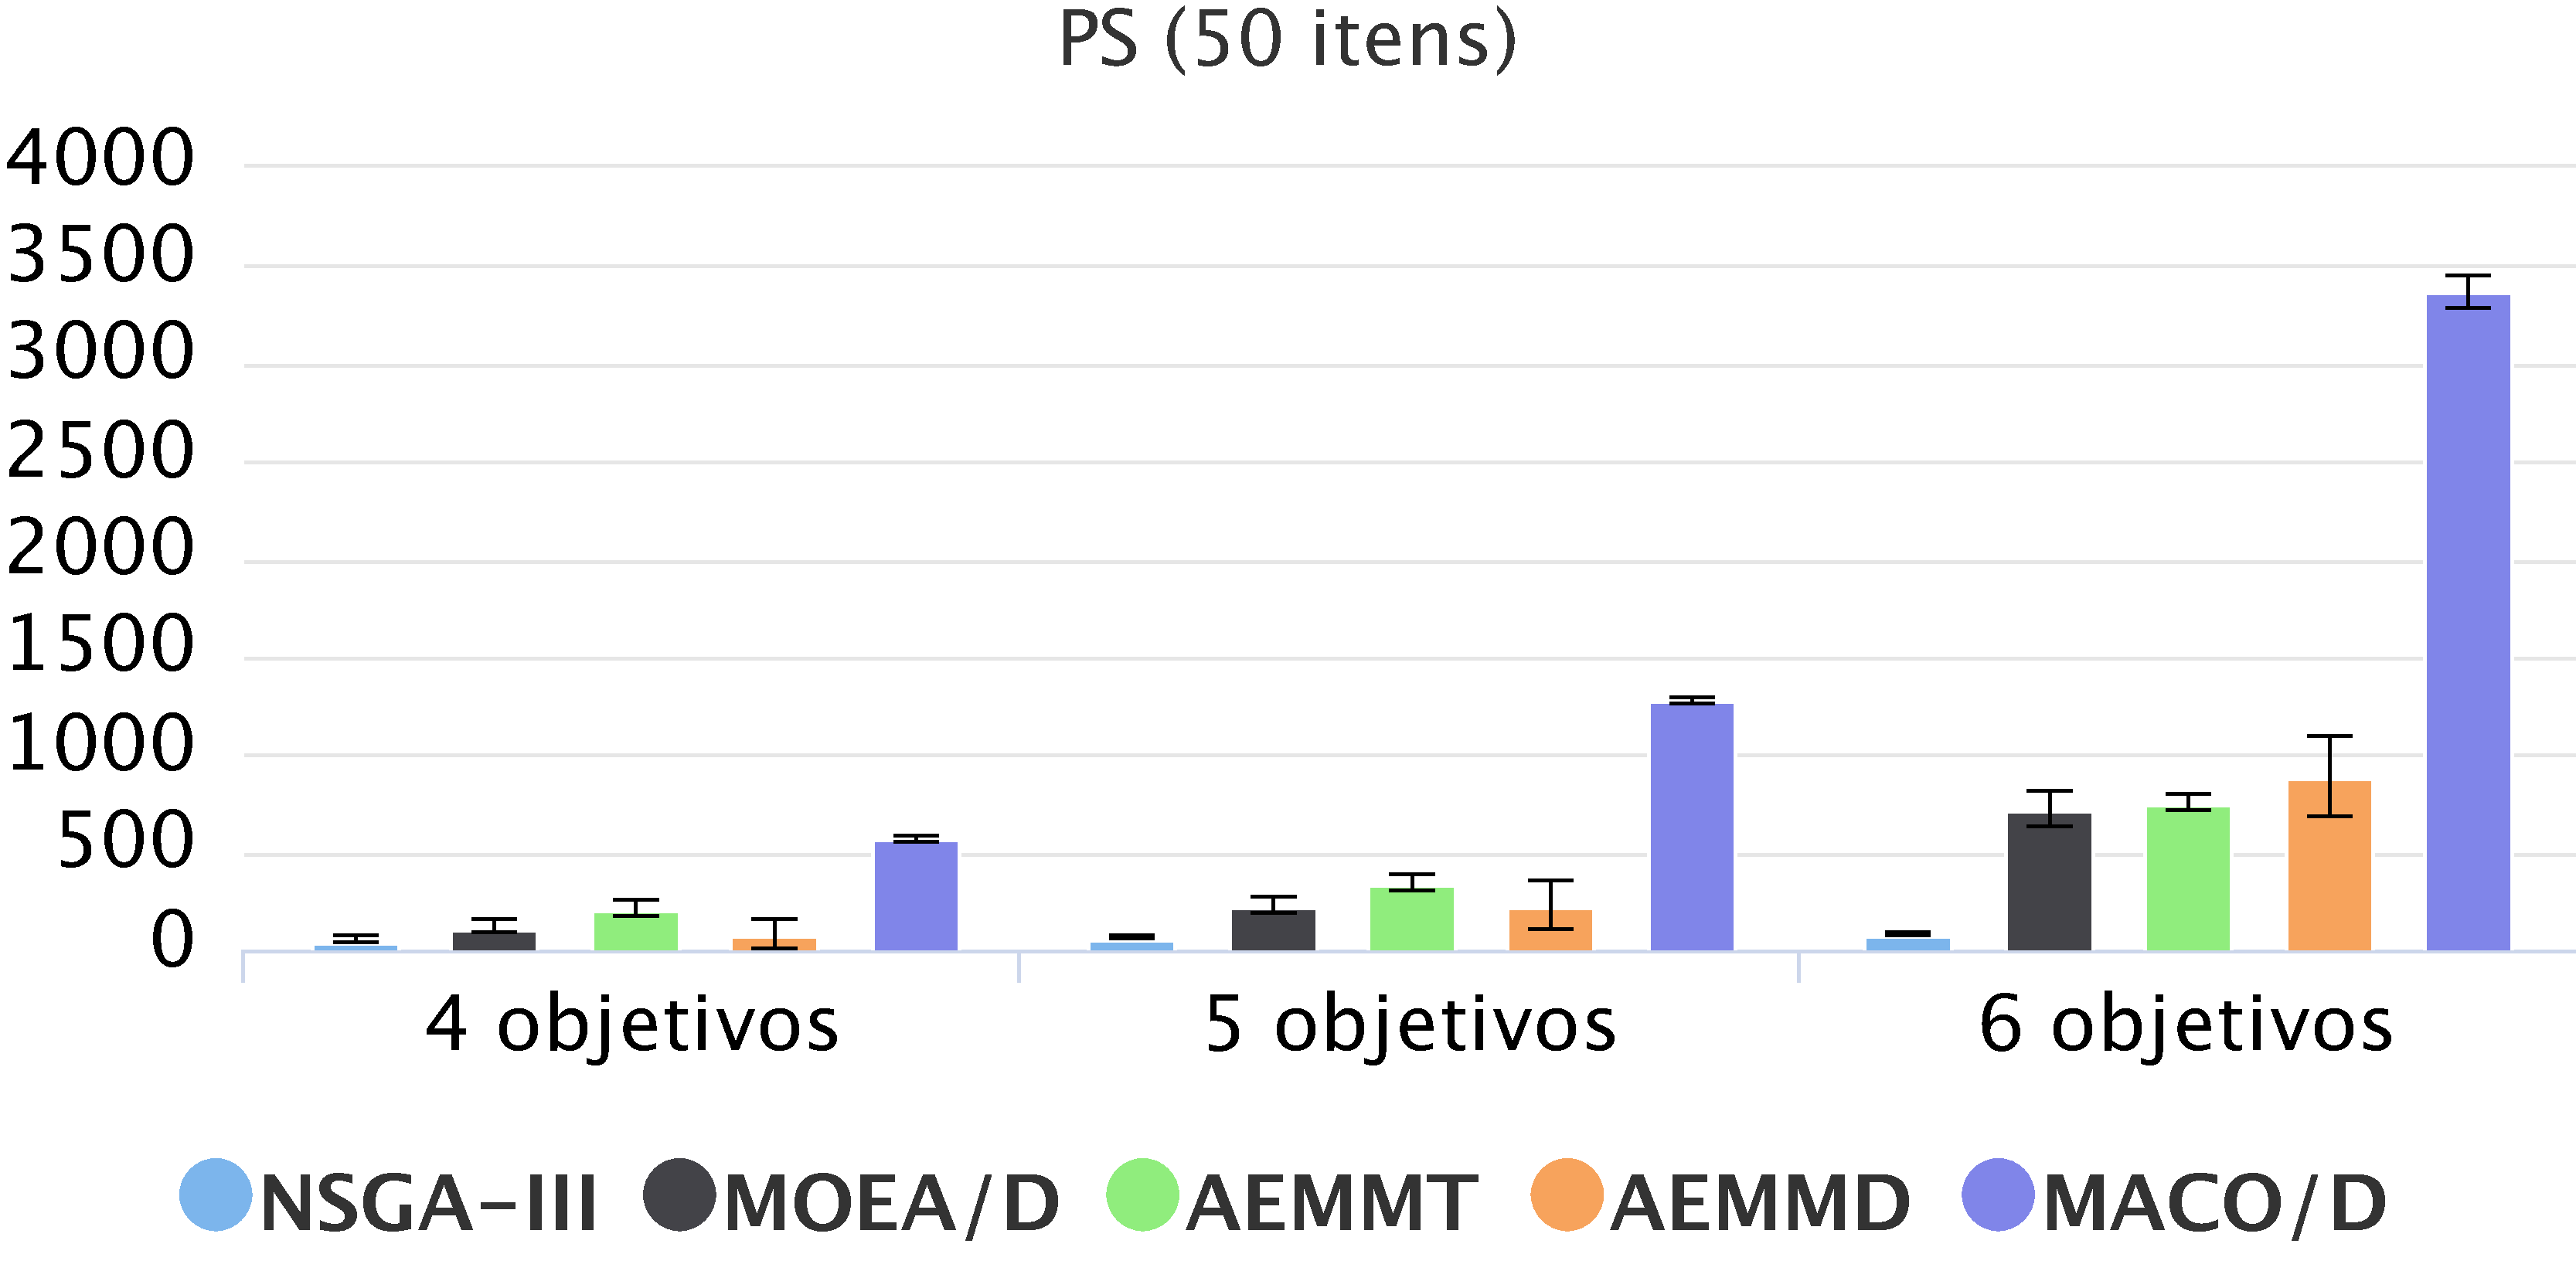
\includegraphics[width=0.5\textwidth]{cap_experimentos/figs/etapa3/ps-mkp-50}
	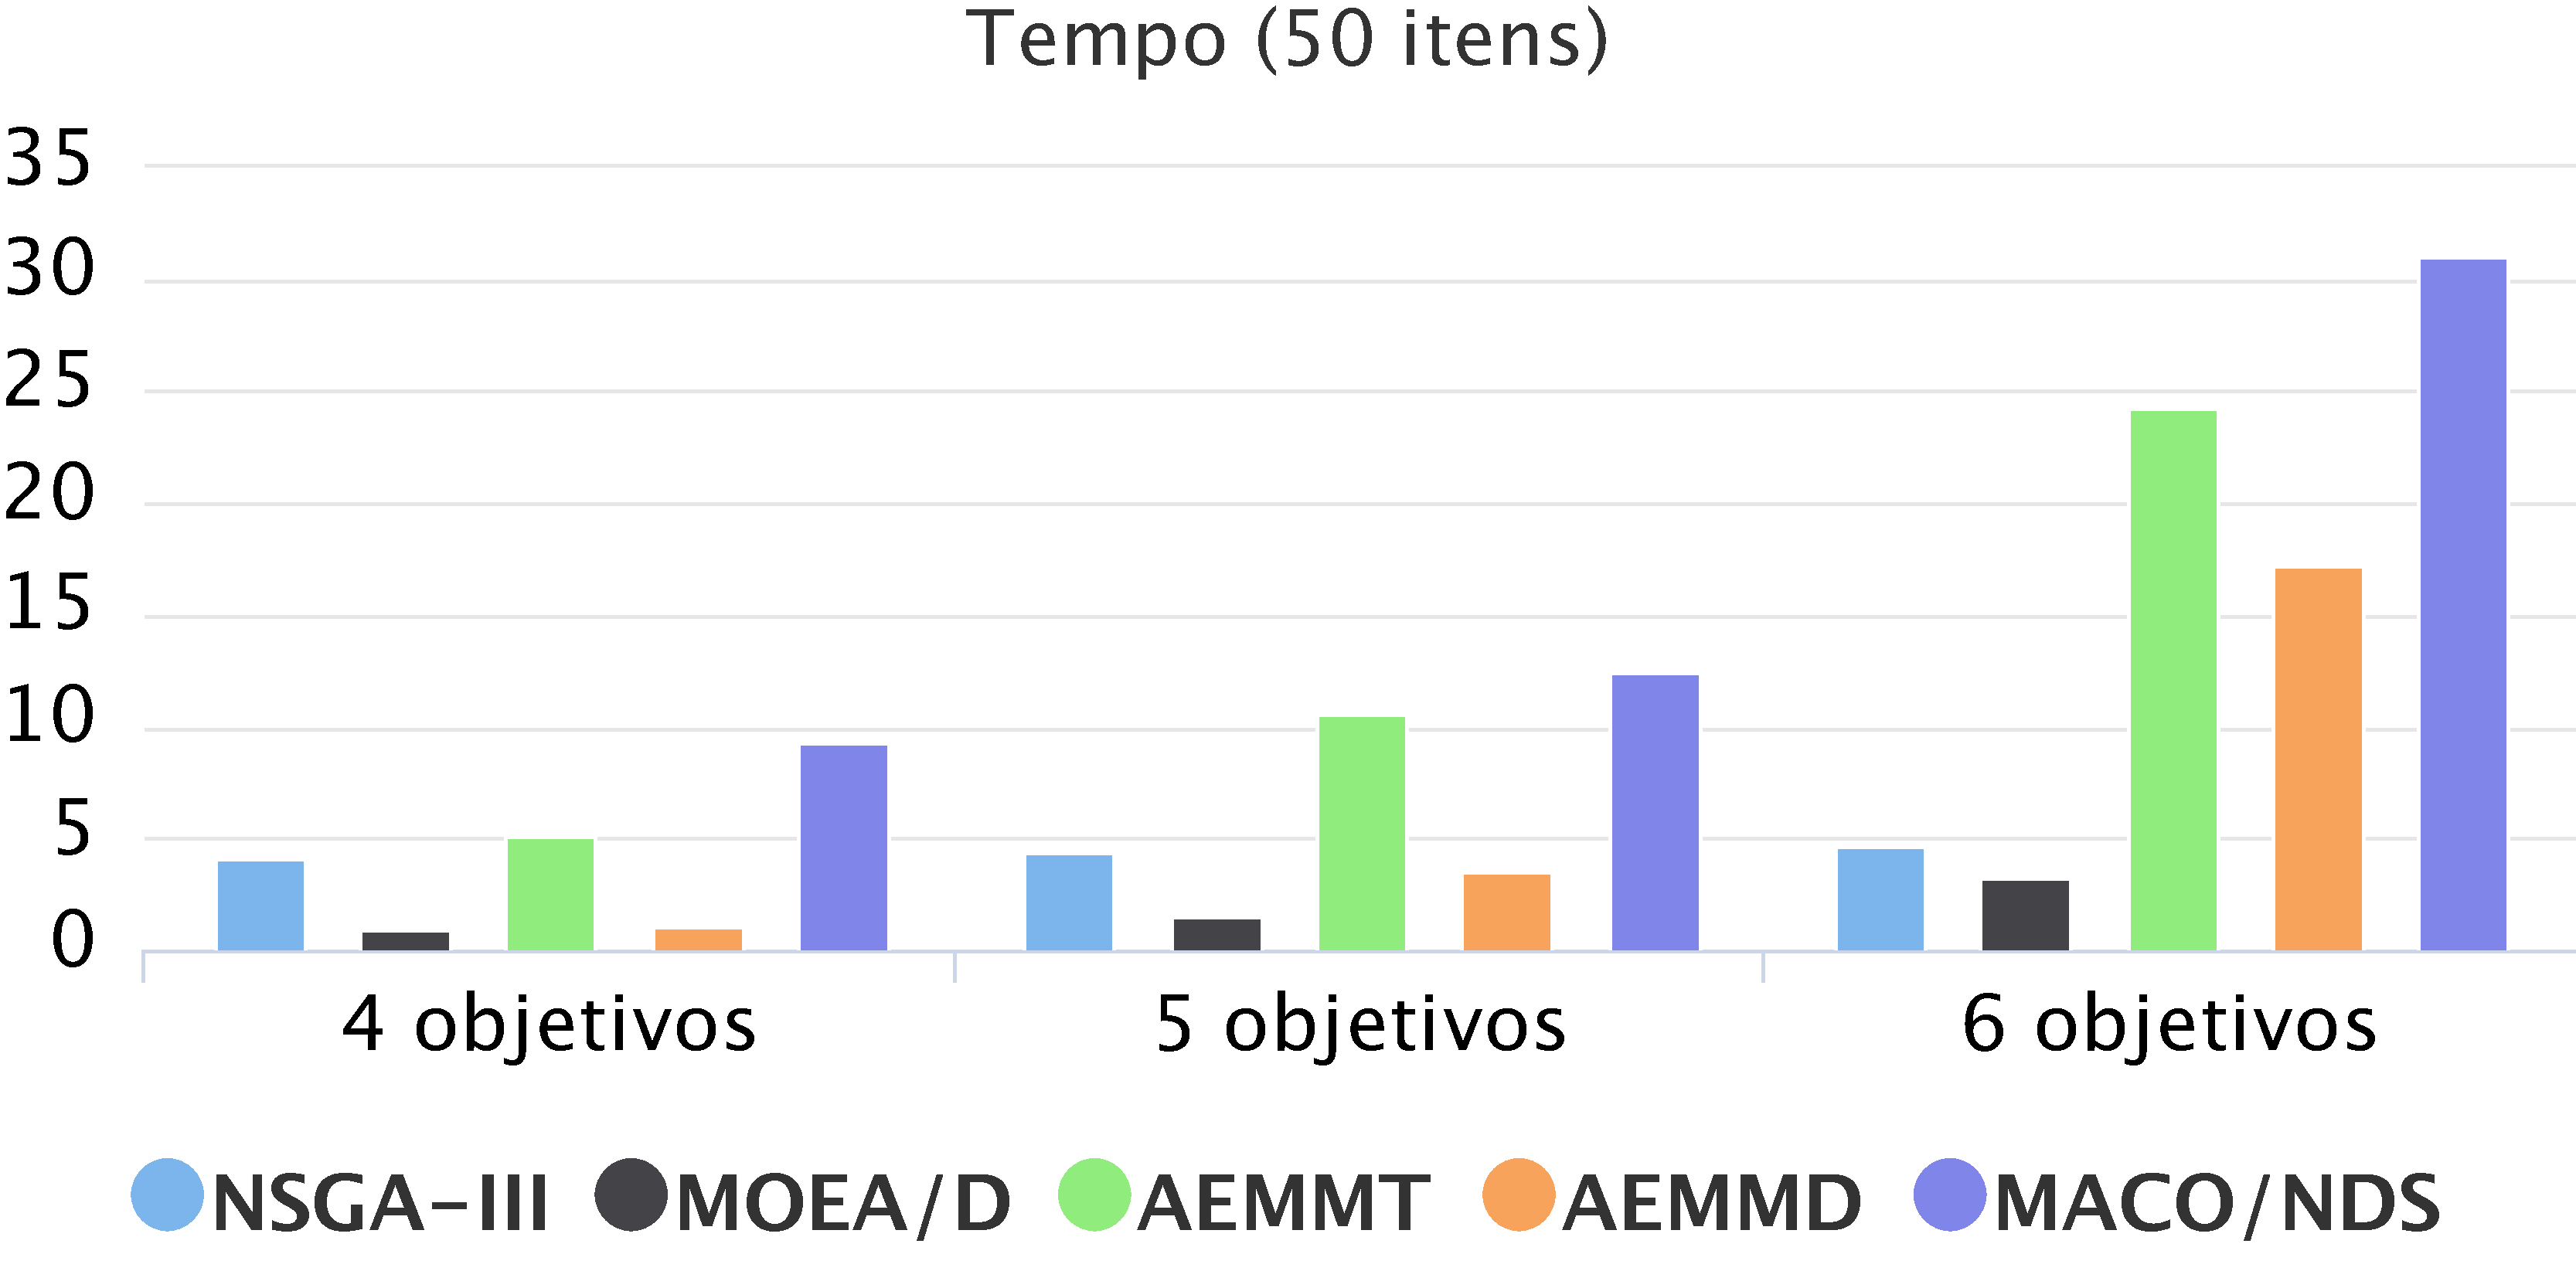
\includegraphics[width=0.5\textwidth]{cap_experimentos/figs/etapa3/time-mkp-50}
	\caption{\label{fig_exp3_pmm_50}Desempenho dos algoritmos na 3ª etapa para o PMM com 50 itens}
\end{figure*}

A \autoref{fig_exp3_pmm_50} mostra o desempenho dos algoritmos no PMM com 50 itens. Como pode ser observado, com exceção do GDp, as demais métricas apresentaram um comportamento similar ao das instâncias anteriores. O MACO/NDS e o AEMMT continuam sendo os algoritmos com menores taxas de erro. Enquanto o MACO/NDS consegue menor $ER$ em 4 e 5 objetivos, o AEMMT apresenta melhor resultado em 6 objetivos. O MACO/NDS obtém os melhores valores de $GDp$ e $PS$, e o MOEA/D é o algoritmo mais rápido. Dentre os algoritmos analisados, o MACO/NDS é o que apresenta o melhor compromisso entre as métricas e a melhor estabilidade quanto à qualidade de soluções (menor desvio padrão).

%!!todo!! Mudar o nome do MACO/NDS nas figuras
\begin{figure*}[!htbp]
	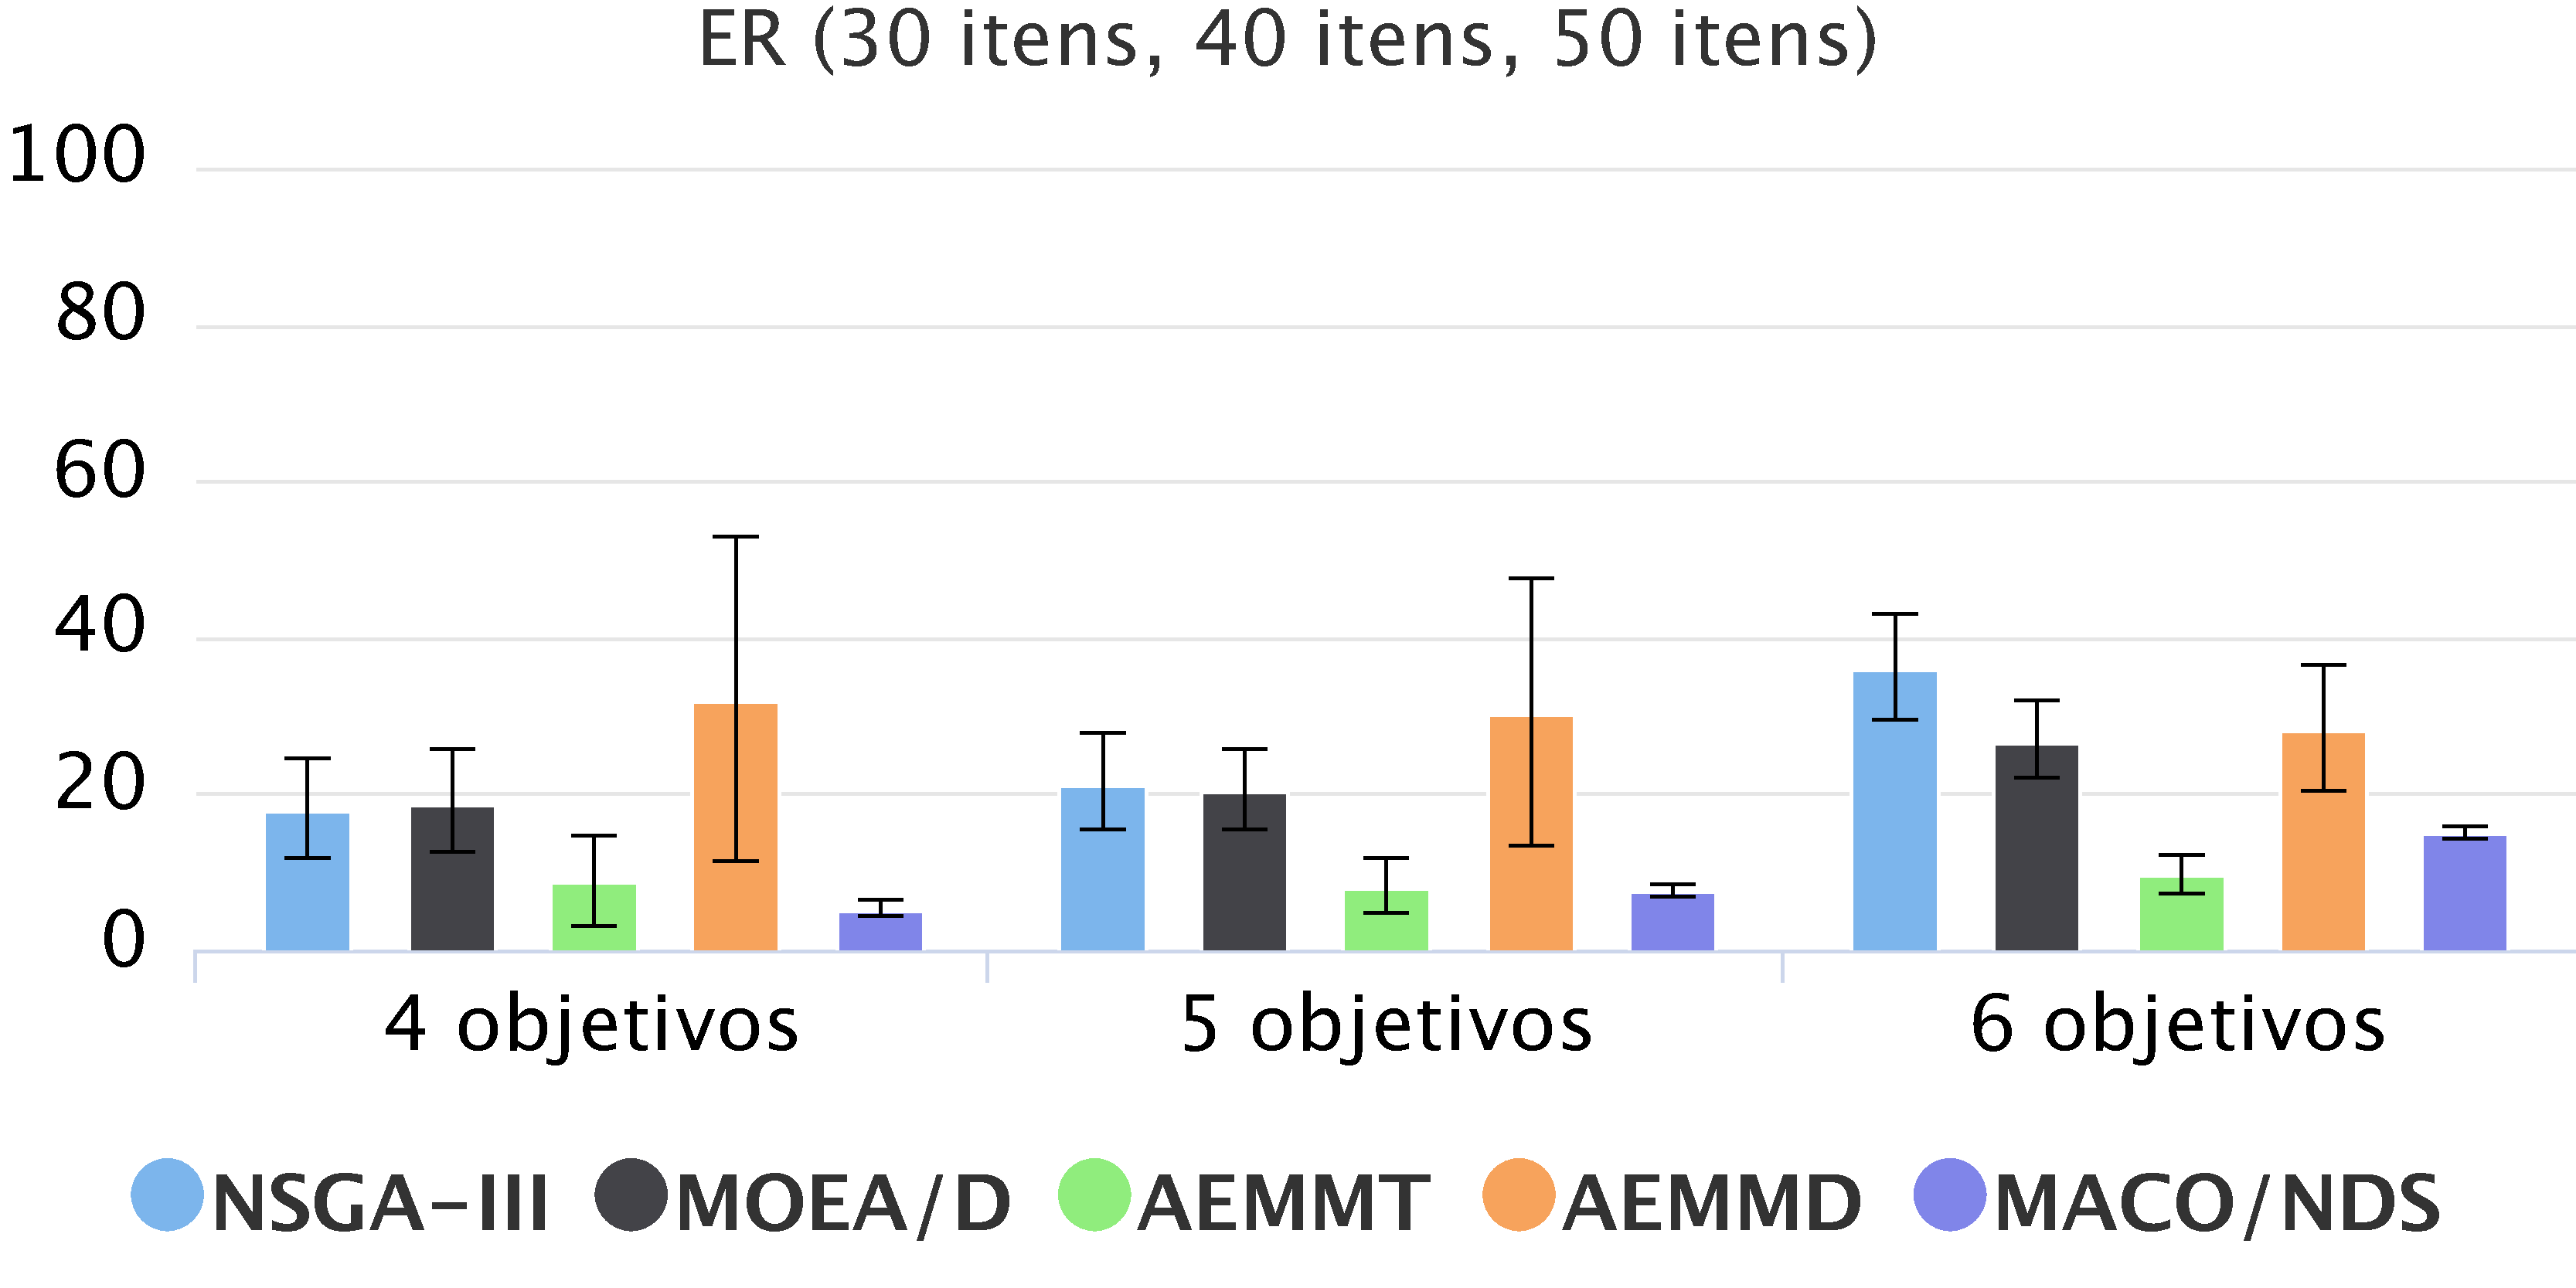
\includegraphics[width=0.5\textwidth]{cap_experimentos/figs/etapa3/er-mkp-todos}
	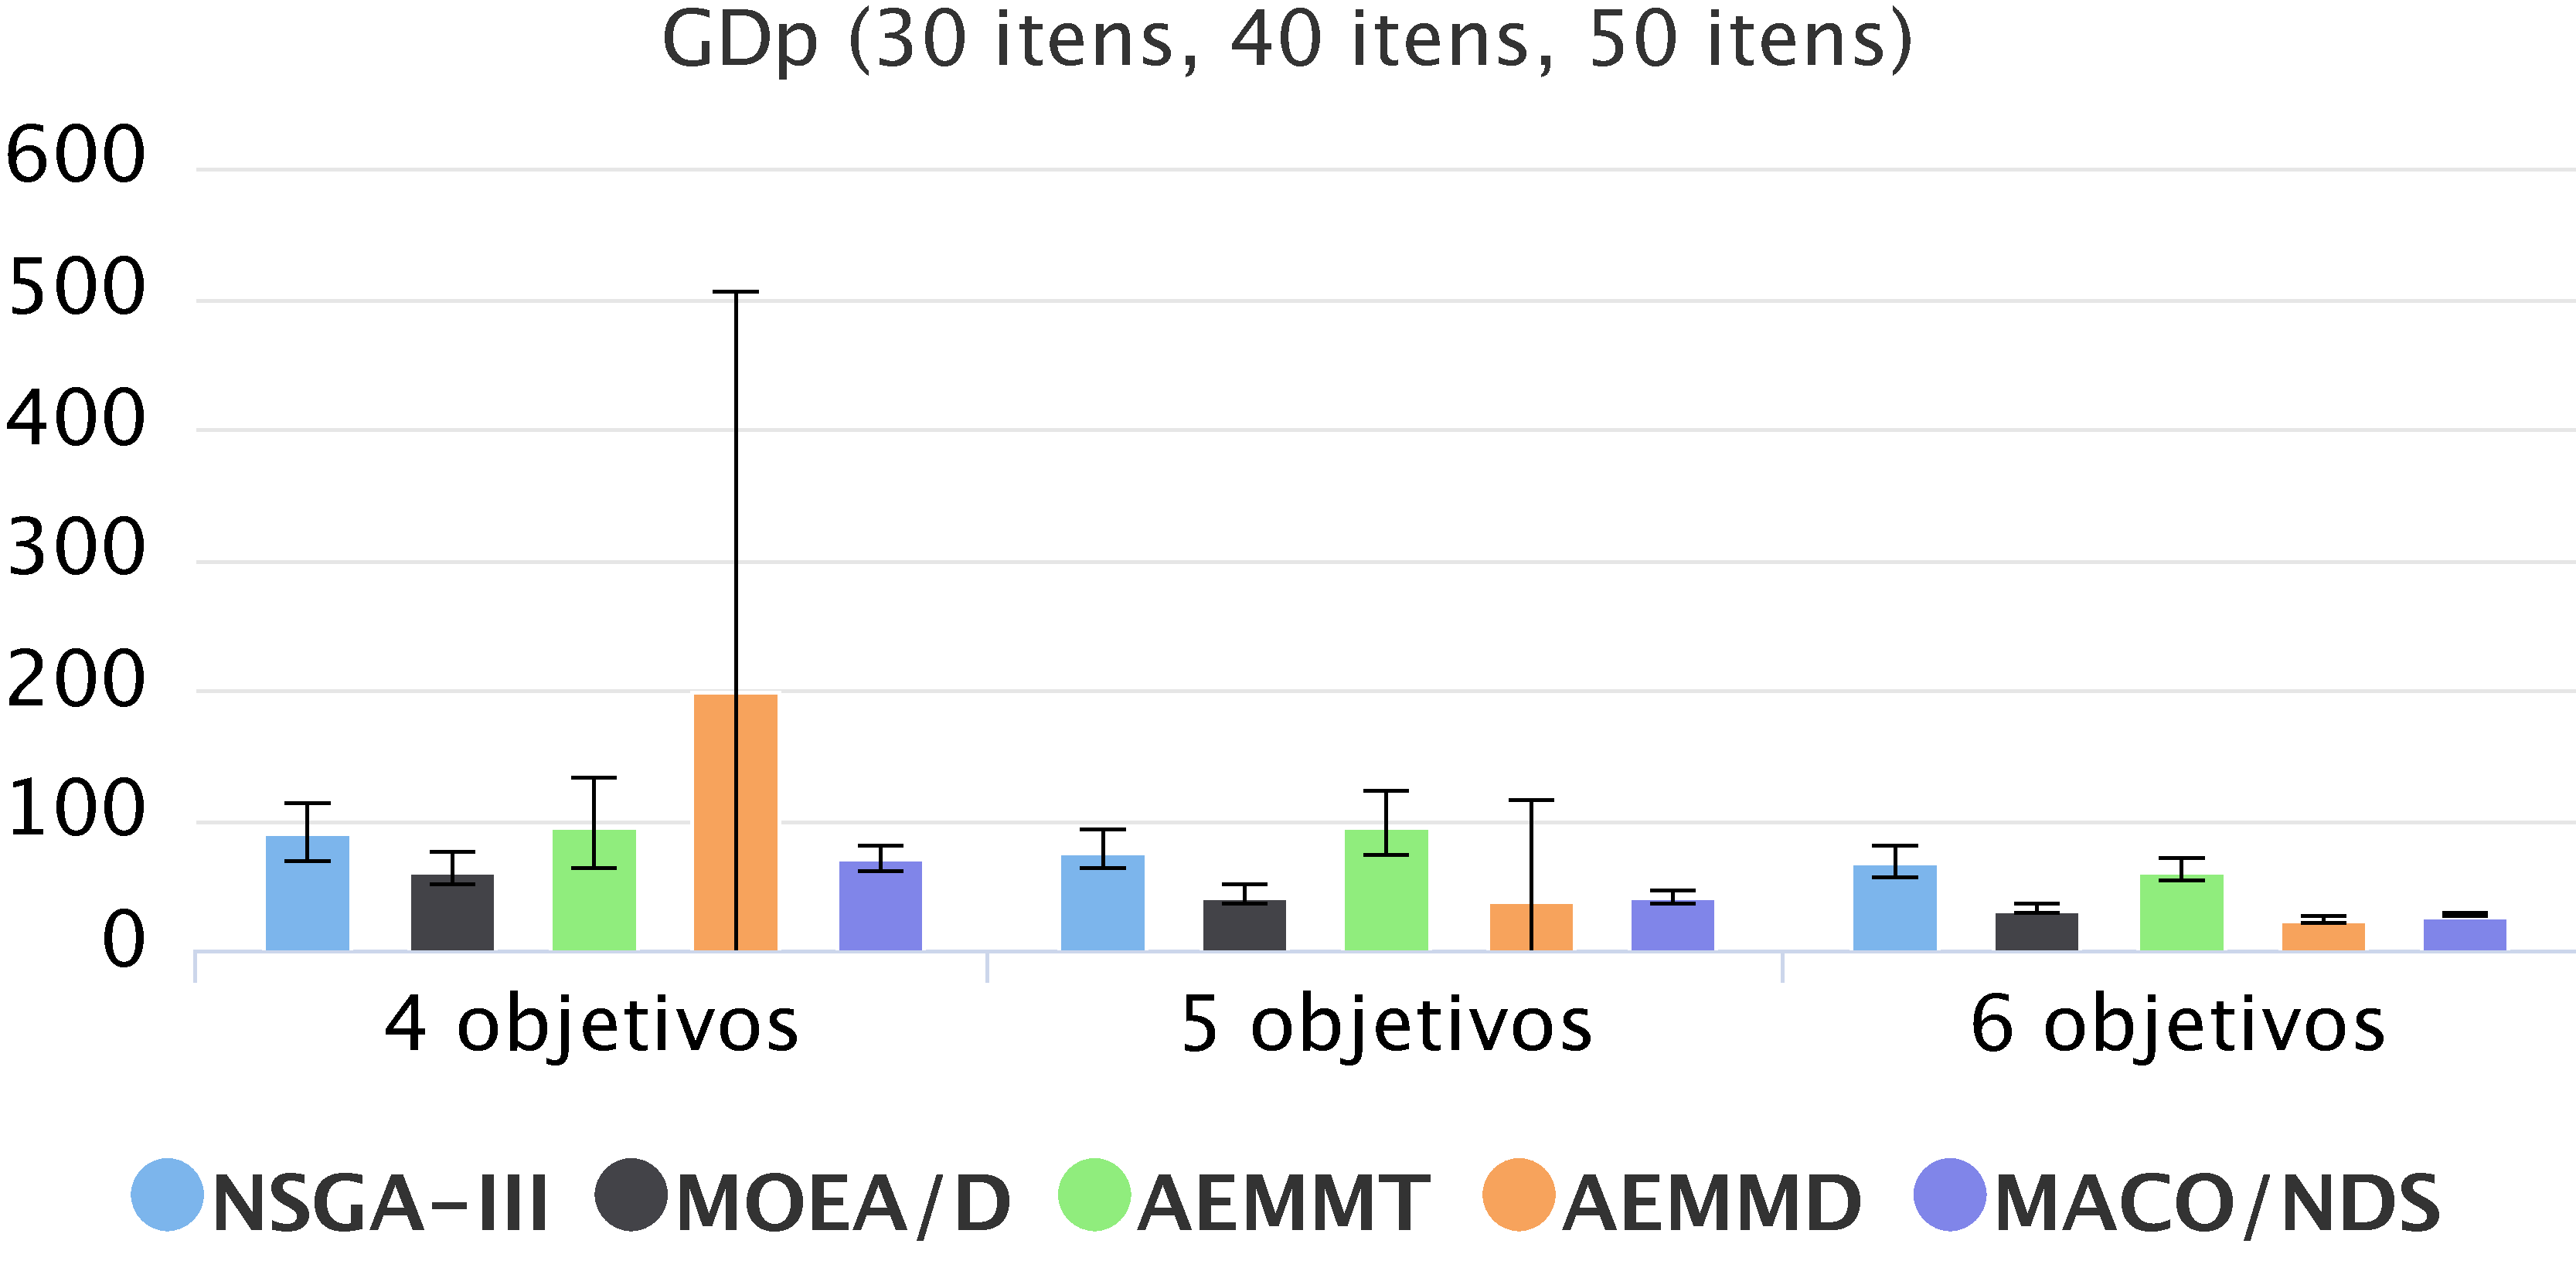
\includegraphics[width=0.5\textwidth]{cap_experimentos/figs/etapa3/gd-mkp-todos}
	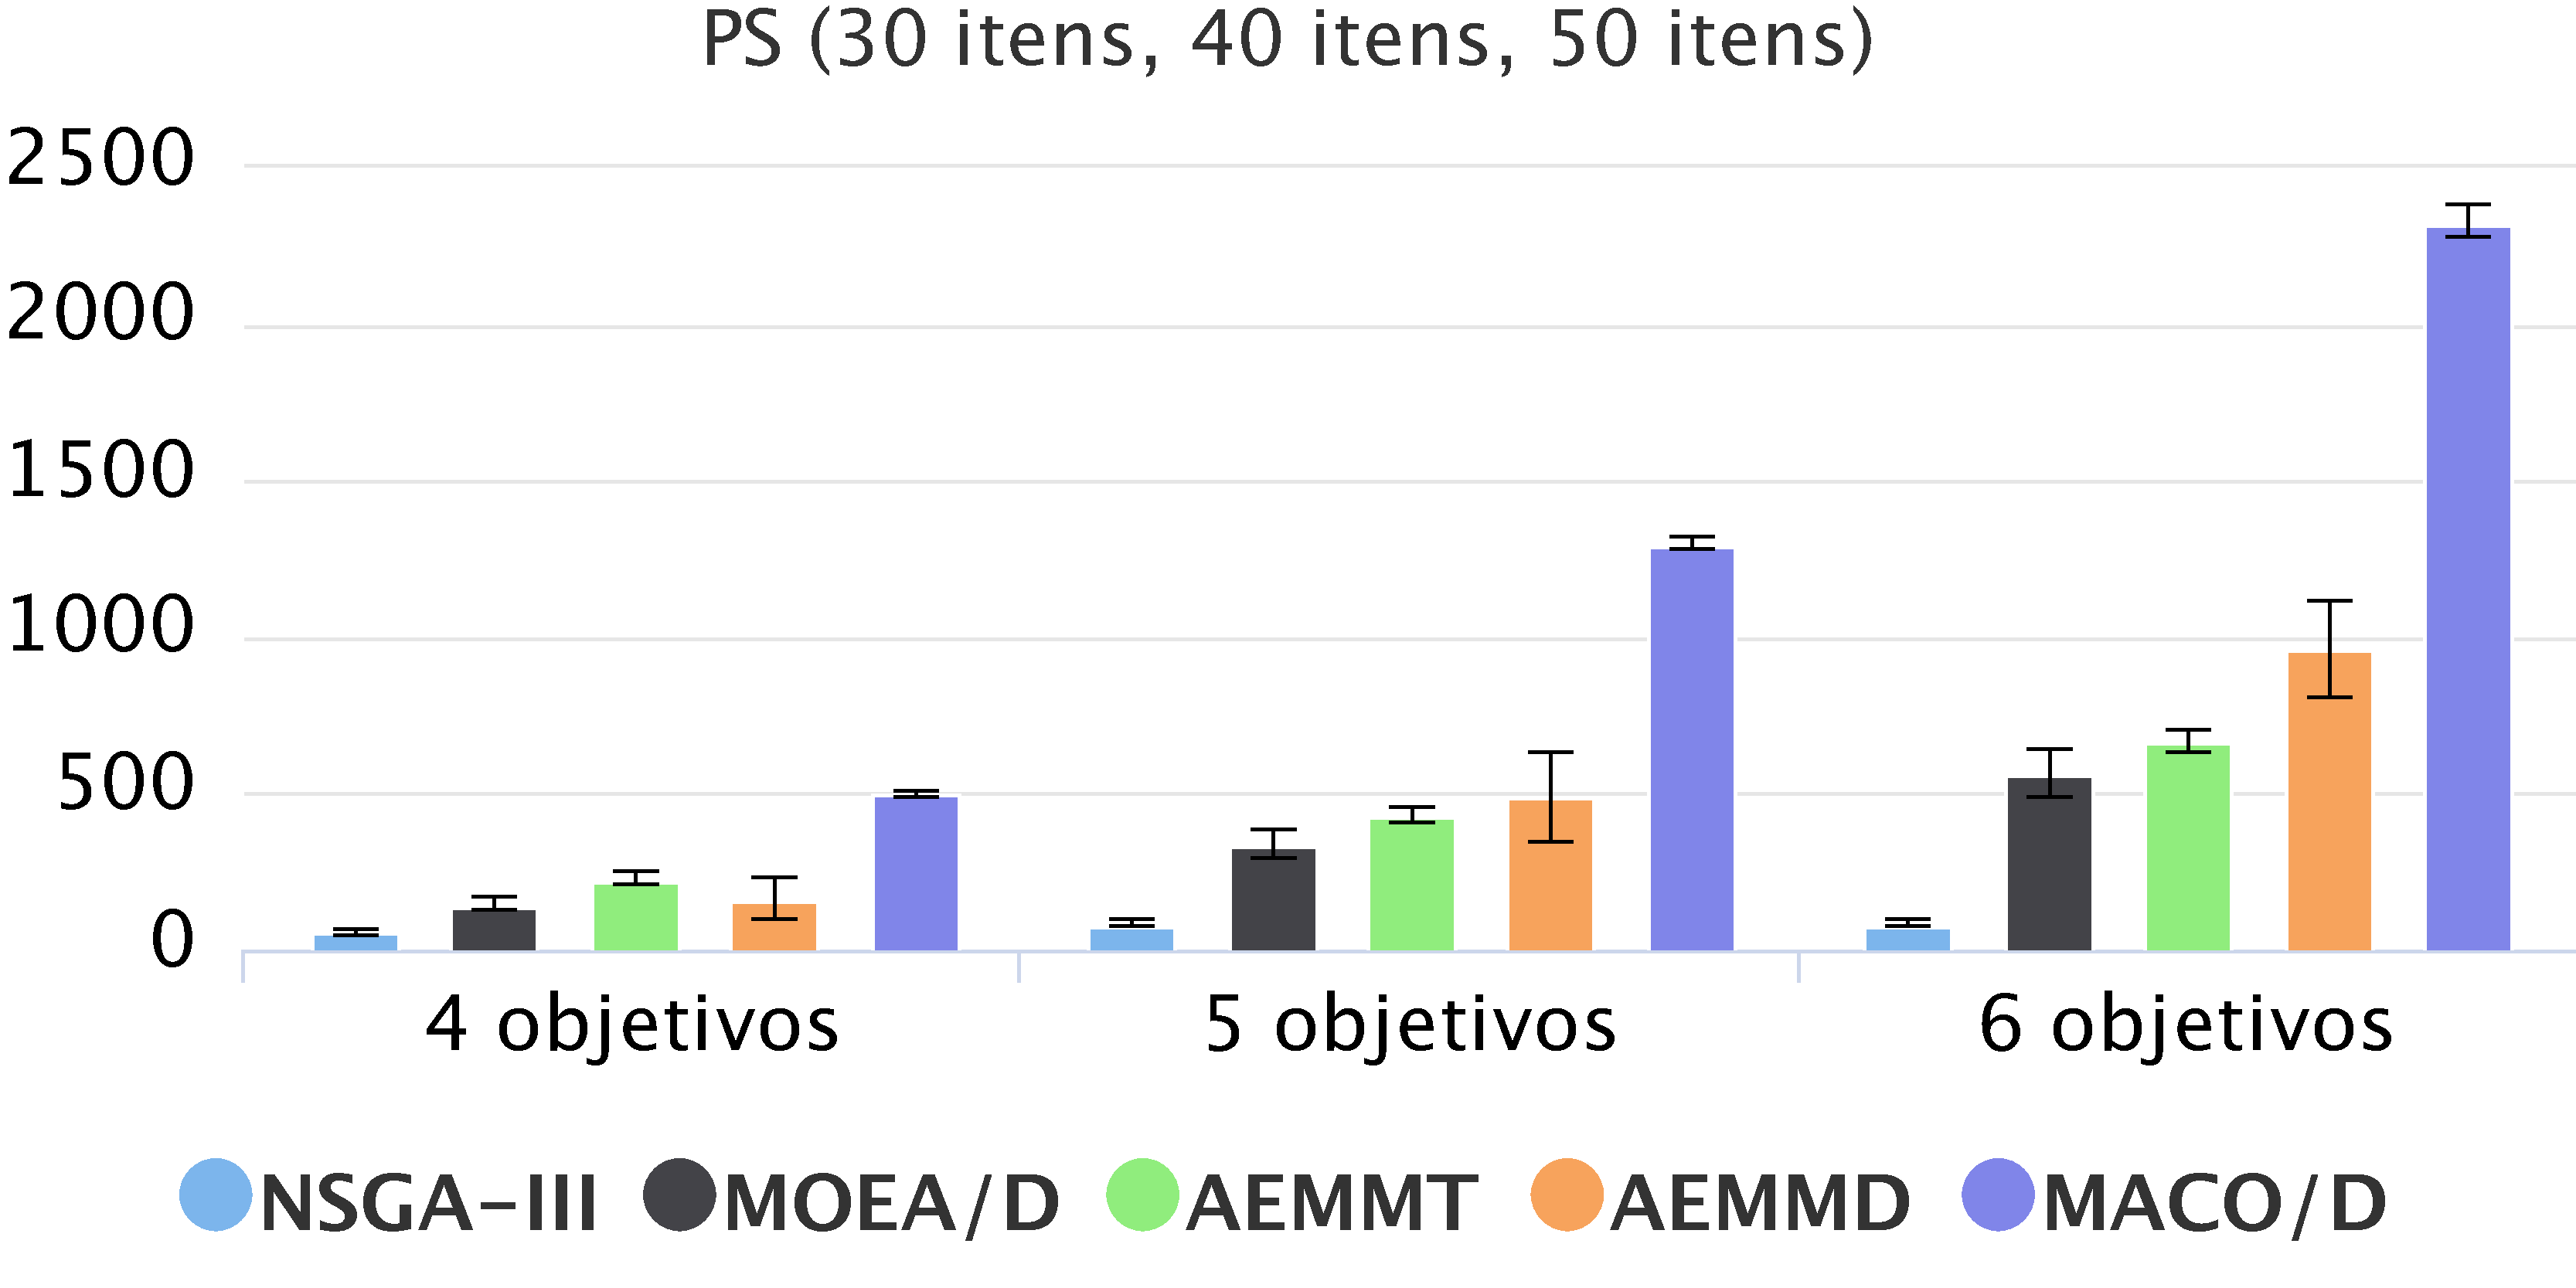
\includegraphics[width=0.5\textwidth]{cap_experimentos/figs/etapa3/ps-mkp-todos}
	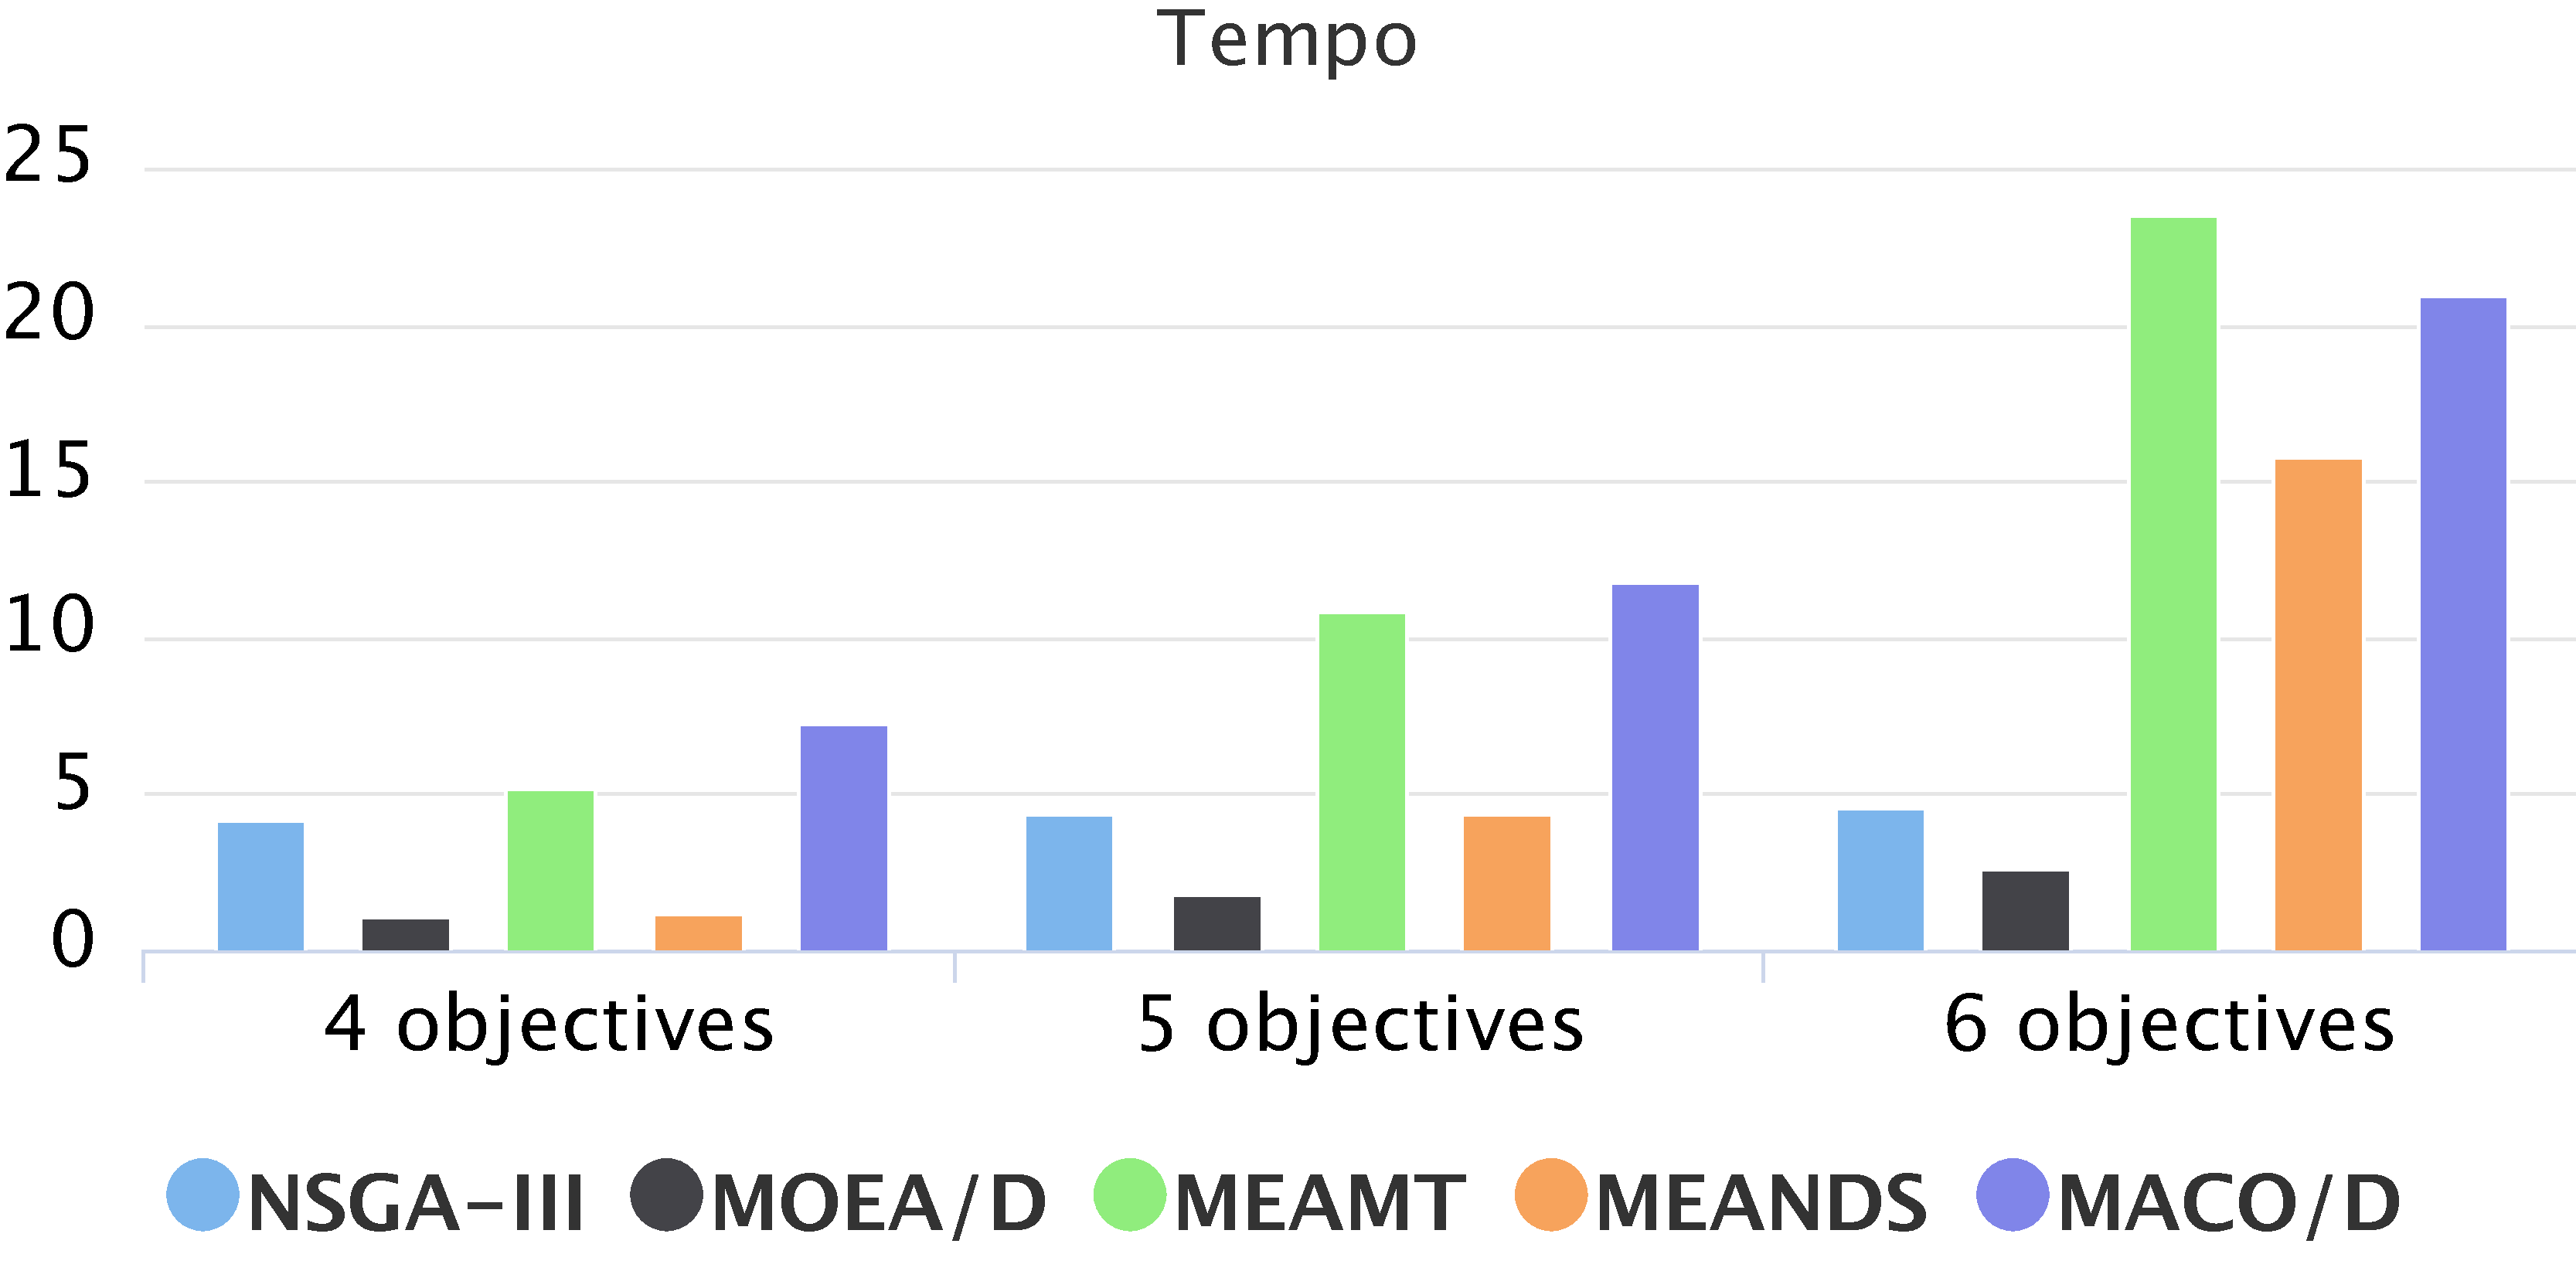
\includegraphics[width=0.5\textwidth]{cap_experimentos/figs/etapa3/time-mkp-todos}
	\caption{\label{fig_exp3_pmm_todos}Resultado consolidado da 3ª etapa considerando o PMM com 30, 40 e 50 itens}
\end{figure*}

A fim de se fazer uma análise geral dos resultados, a média entre os 3 cenários é apresentada nos gráficos da \autoref{fig_exp3_pmm_todos}. As taxas de erro são muito baixas para o AEMMT e o MACO/NDS, quando comparados aos demais algoritmos. Os resultados em $GDp$ são bons para a maioria dos métodos. Apenas o AEMMD apresenta um valor alto de $GDp$ e com elevado desvio padrão para o problema de 4 objetivos (200 com desvio padrão de 504). O MOEA/D produz o melhor $GDp$ no problema de 4 objetivos (62,9), enquanto que, para 5 e 6 objetivos, o AEMMD (40,7 para 5 objetivos e 23,6 para 6) e o MACO/NDS (41,1 para 5 objetivos e 26,8 para 6) conseguem valores melhores que o MOEA/D (43 para 5 objetivos e 31,9 para 6), mas ainda similares. É importante notar que os desvios padrões no AEMMD são altos, representando uma certa instabilidade do algoritmo em gerar boas soluções. Em termos da cobertura da fronteira de Pareto ($PS$), o MACO/NDS alcançou os melhores valores em todas as formulações de objetivos. Analisando o tempo de execução médio, o AEMMT, o AEMMD e o MACO/S variam bastante com o número de objetivos, enquanto os demais são estáveis. O MOEA/D é o algoritmo mais rápido entre os avaliados nesta etapa dos experimentos.

\begin{figure*}[!htbp]
	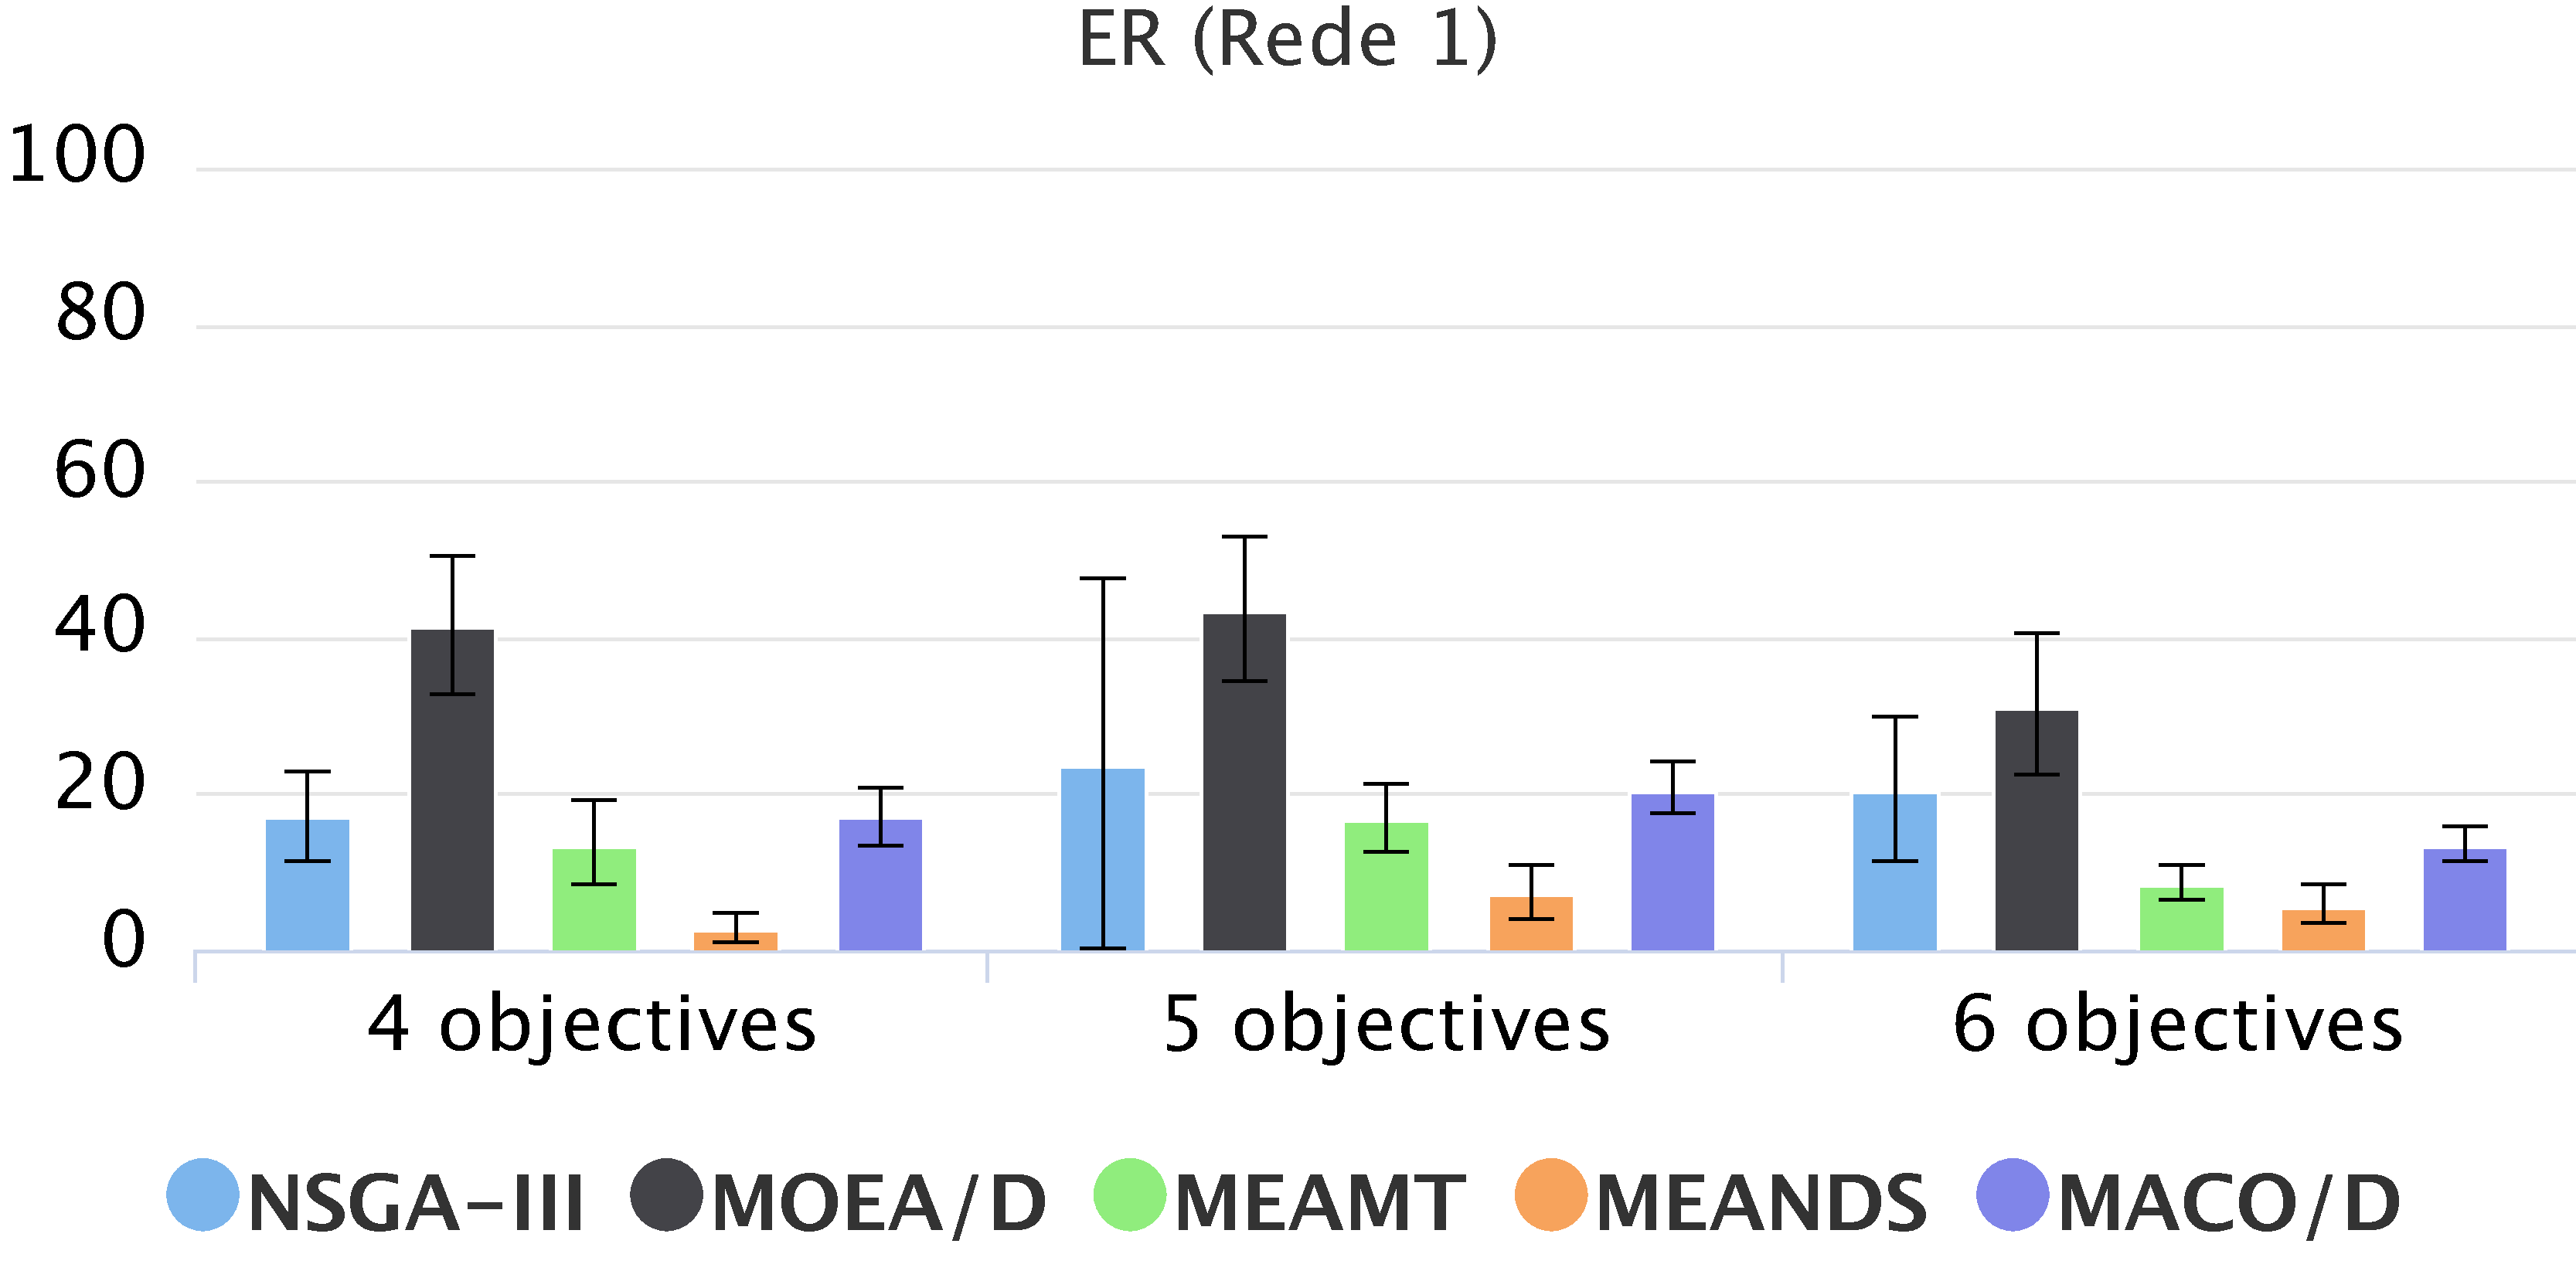
\includegraphics[width=0.5\textwidth]{cap_experimentos/figs/etapa3/er-mrp-r1}
	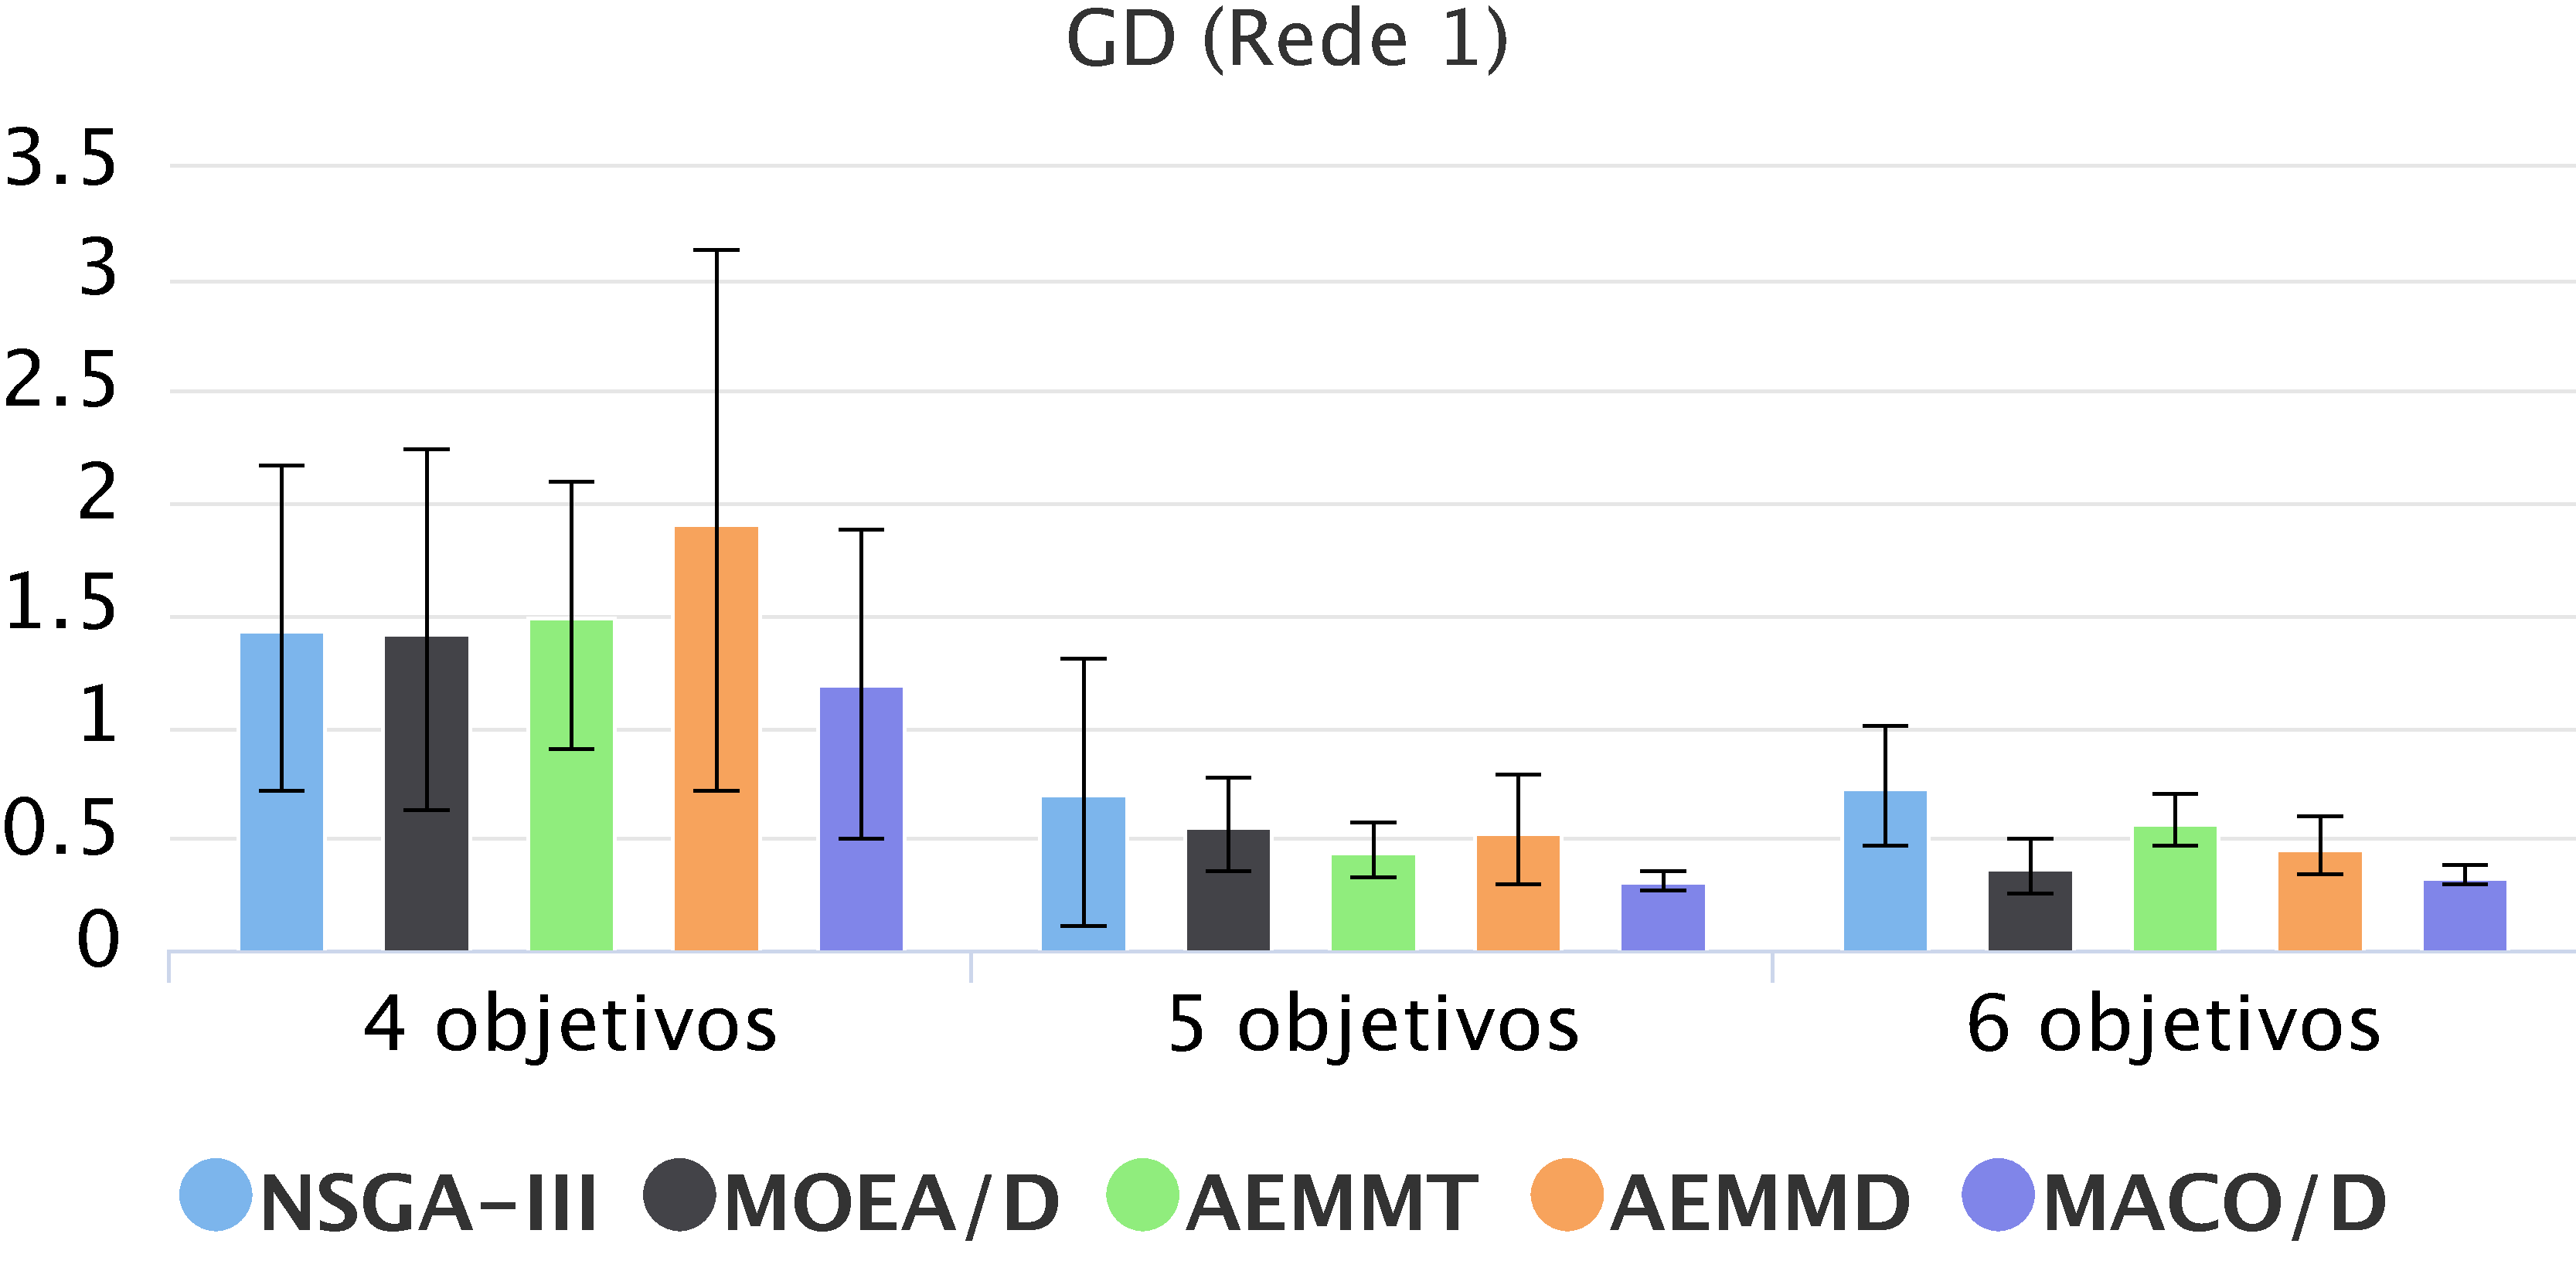
\includegraphics[width=0.5\textwidth]{cap_experimentos/figs/etapa3/gd-mrp-r1}
	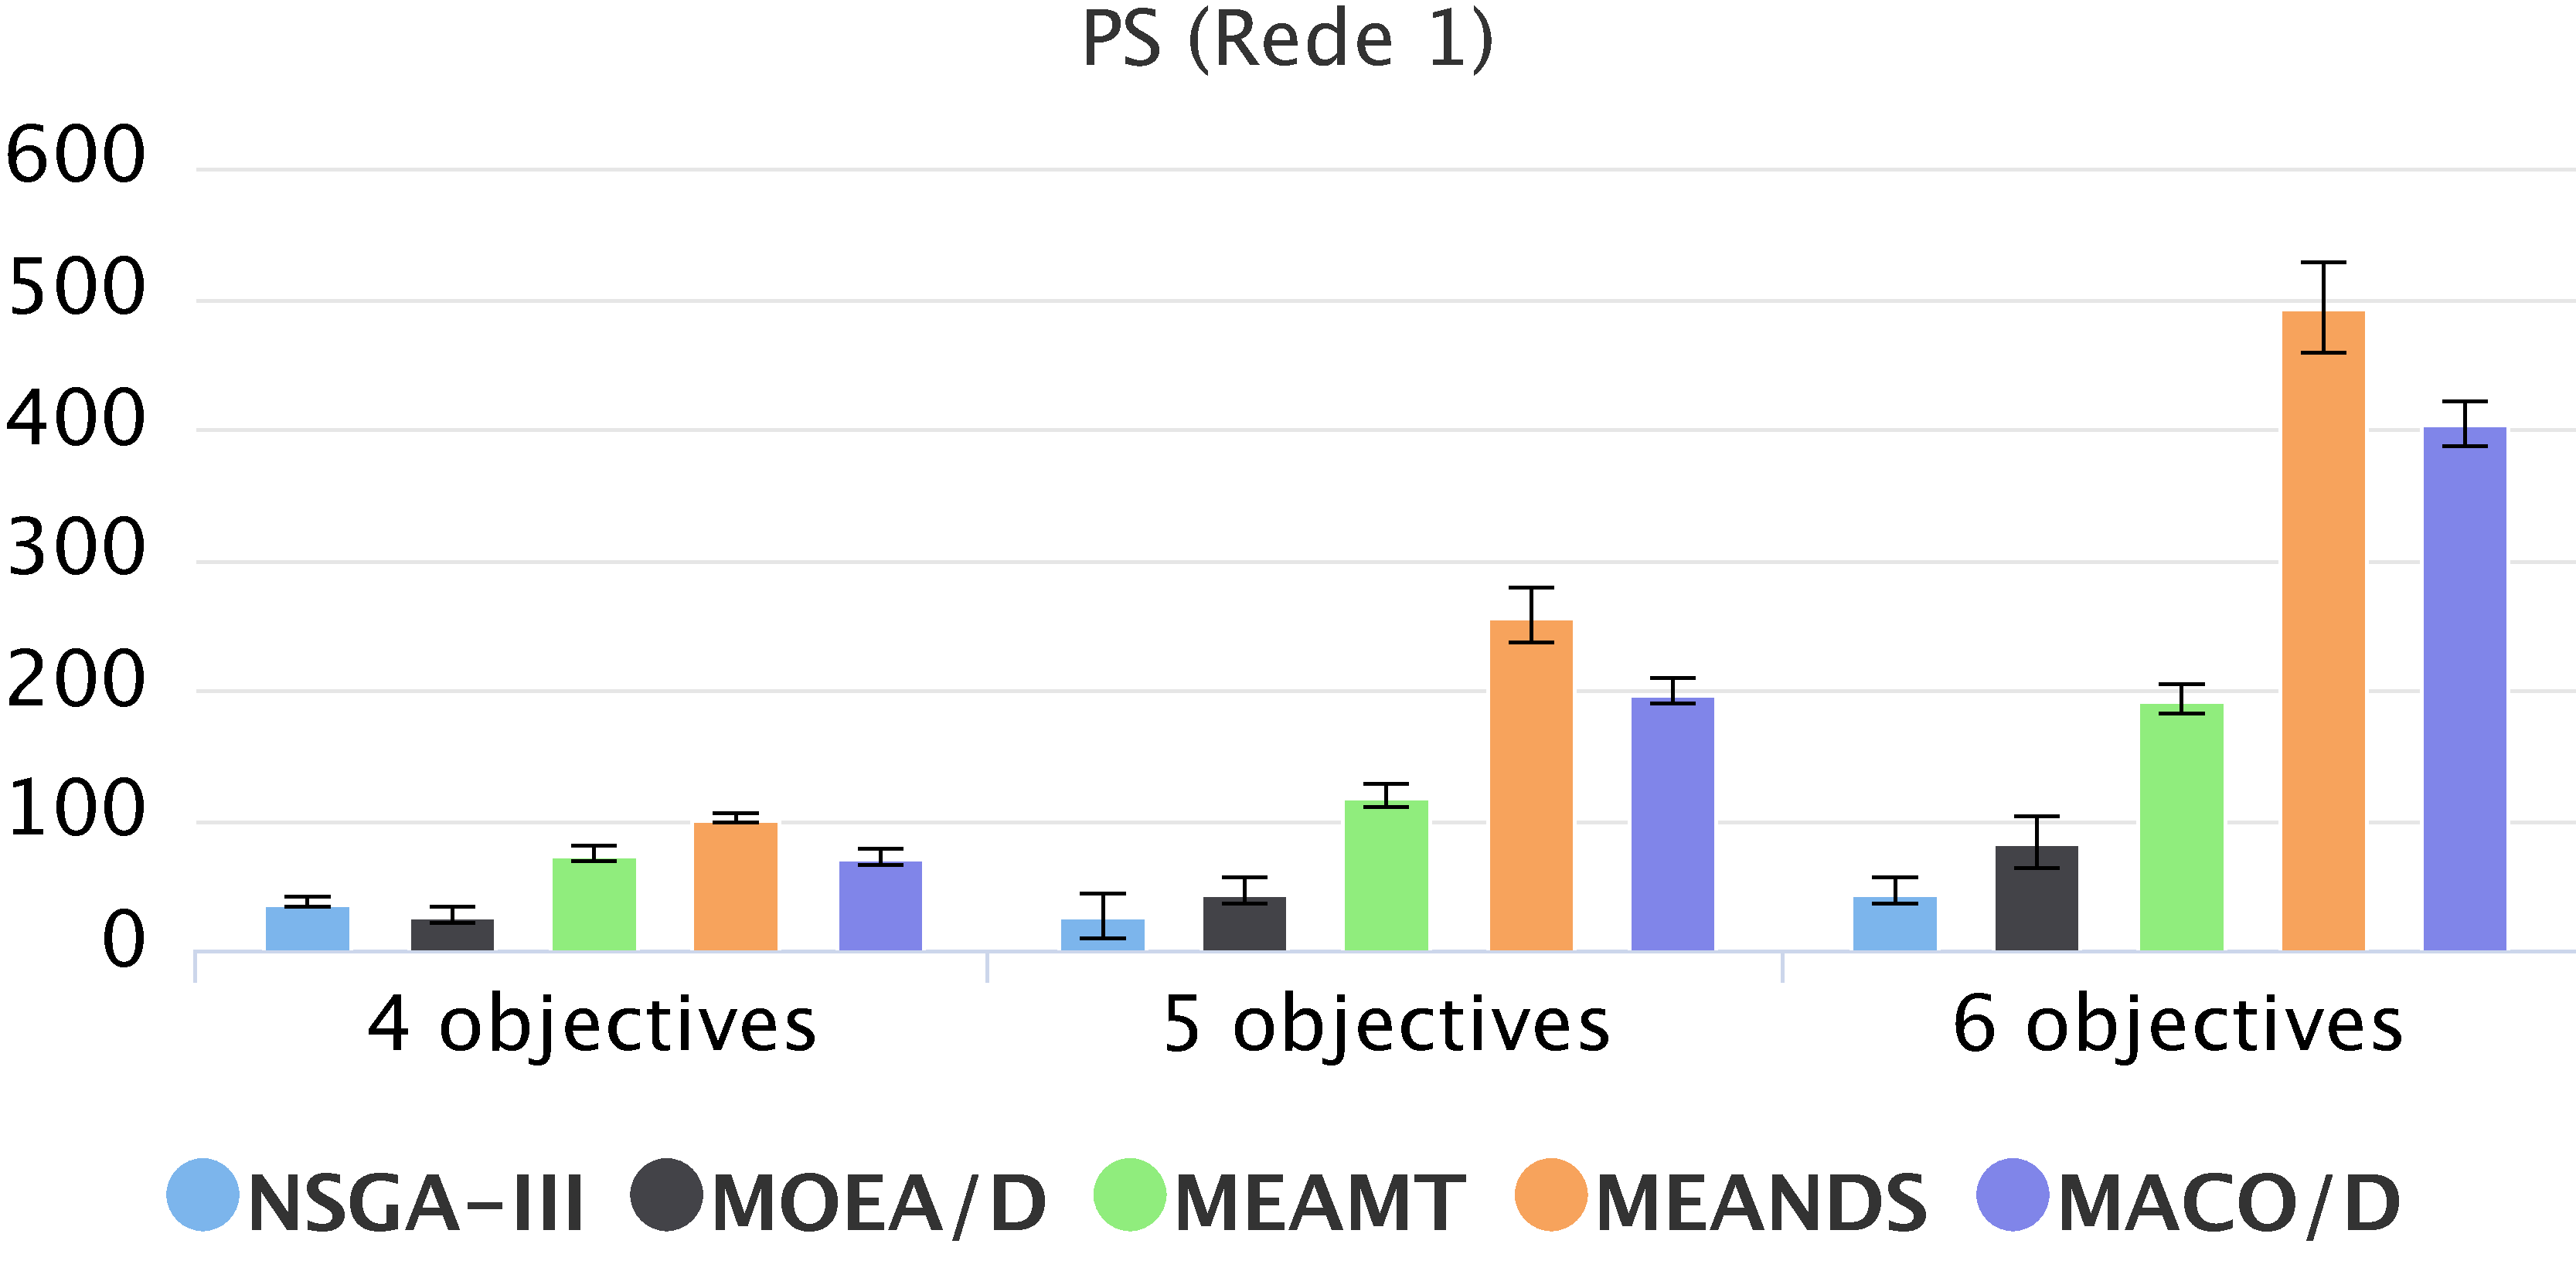
\includegraphics[width=0.5\textwidth]{cap_experimentos/figs/etapa3/ps-mrp-r1}
	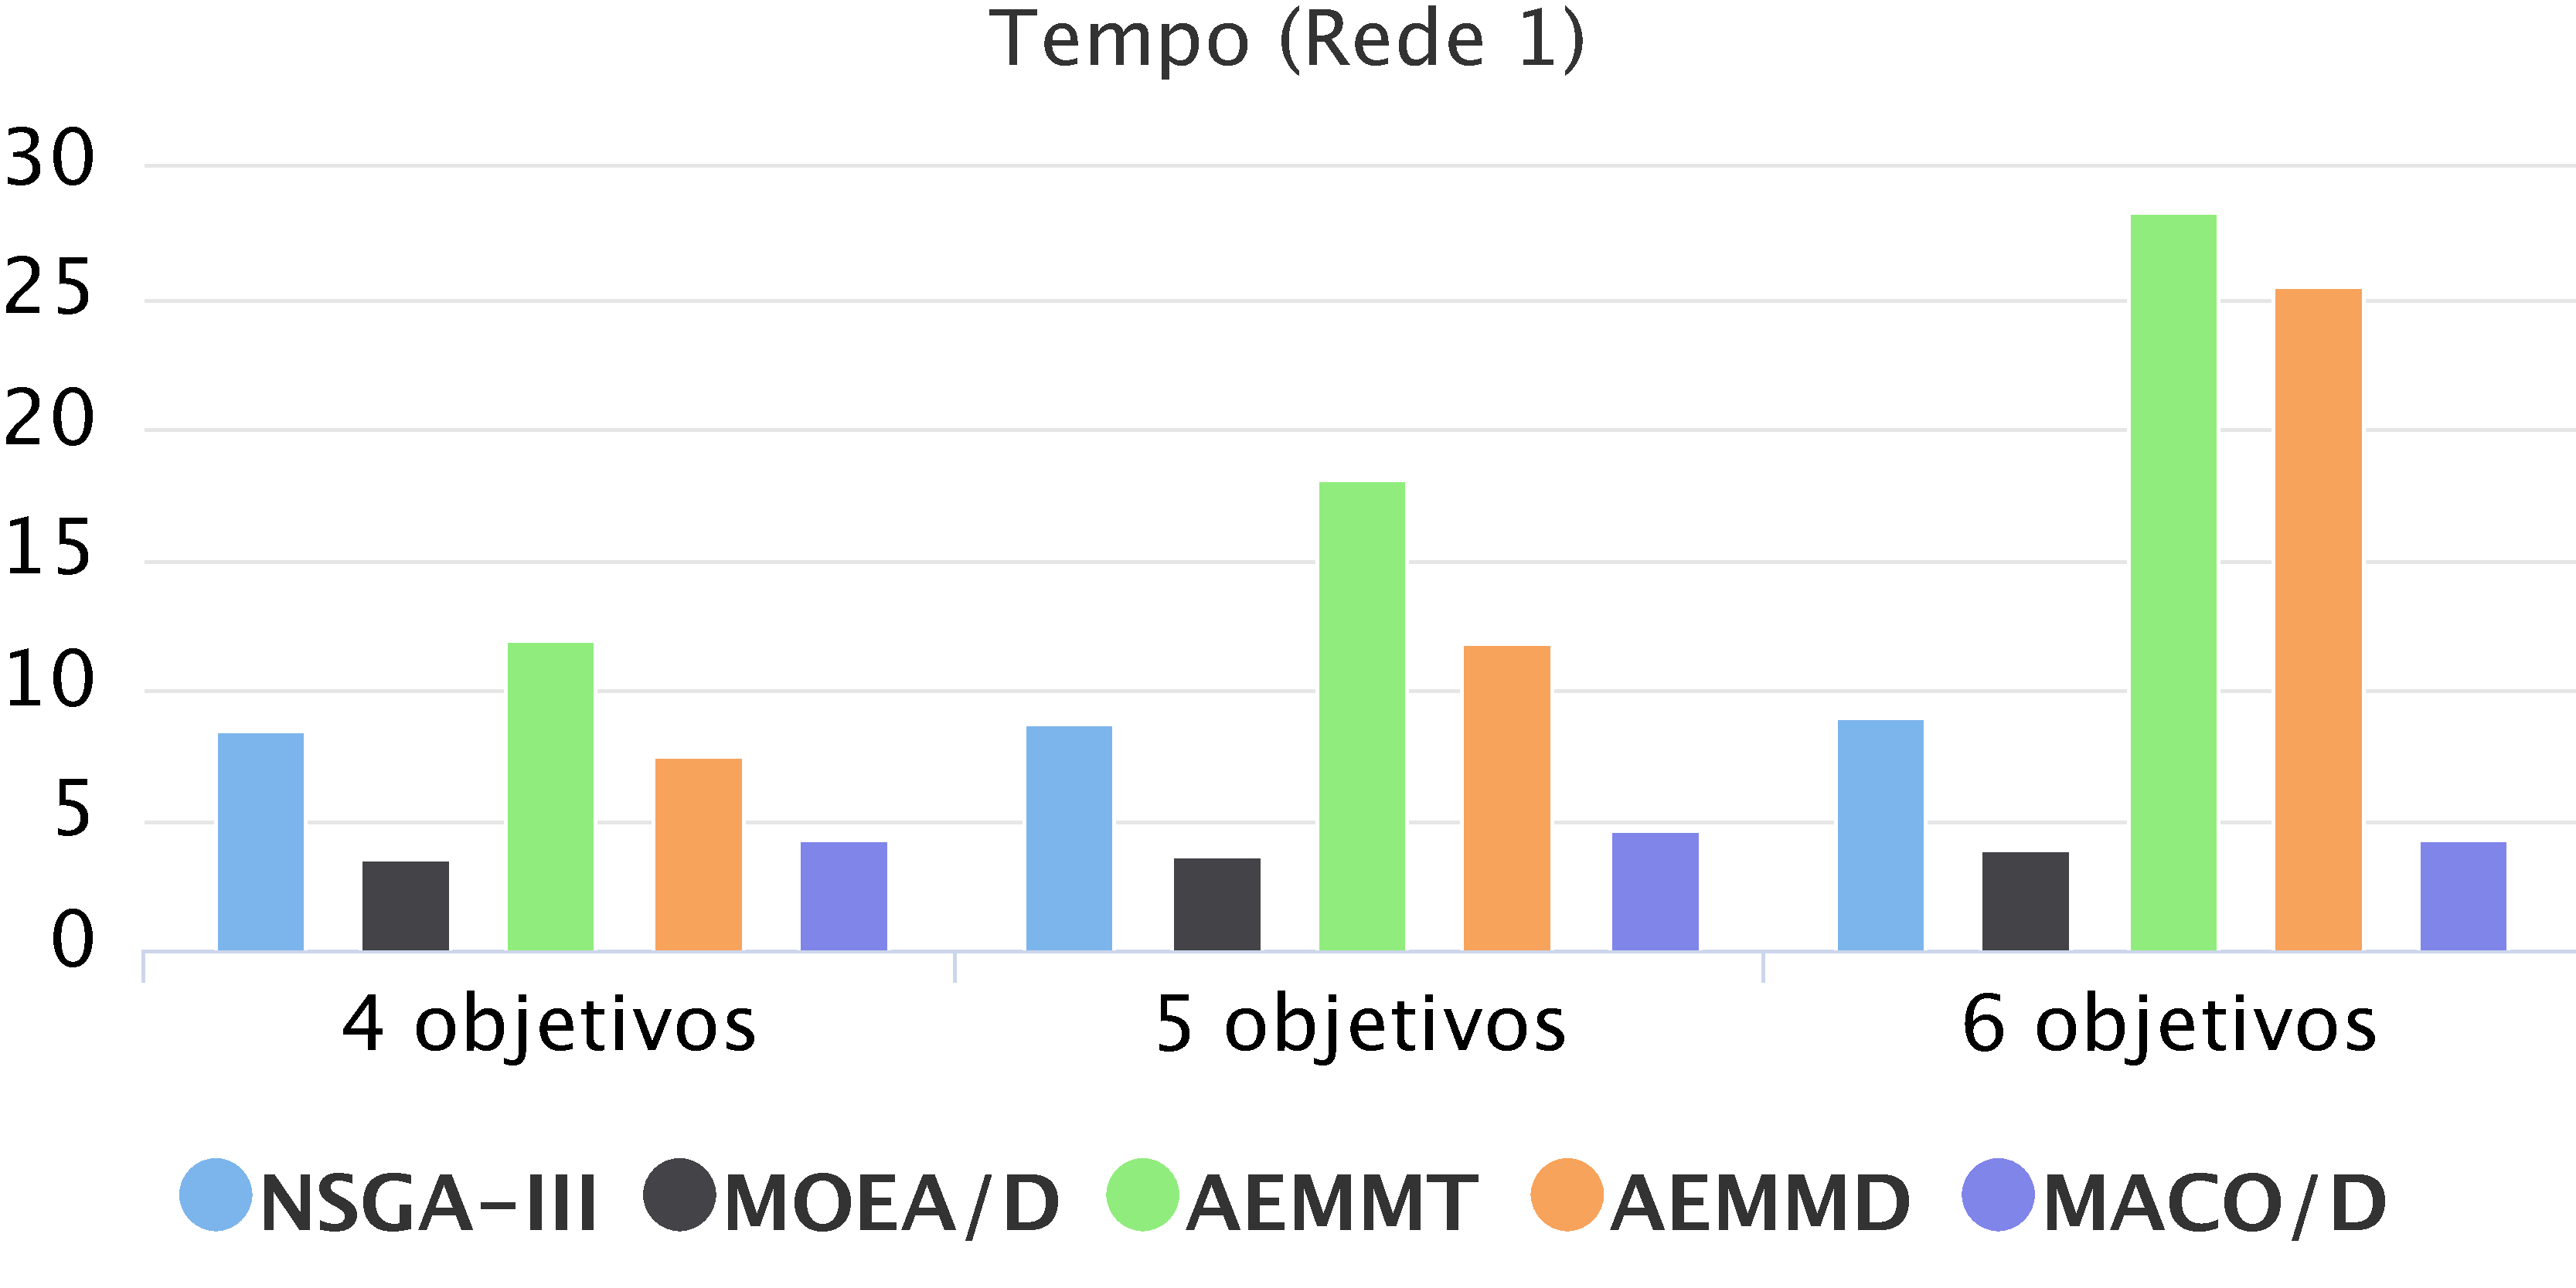
\includegraphics[width=0.5\textwidth]{cap_experimentos/figs/etapa3/time-mrp-r1}
	\caption{\label{fig_exp3_prm_r1}Desempenho dos algoritmos na 3ª etapa para o PRM na rede 1}
\end{figure*}

Os gráficos correspondentes ao PRM na rede 1 são apresentados na \autoref{fig_exp3_prm_r1}. Em relação à taxa de erro, o AEMMD obtém os menores valores em todas as formulações de objetivos. Em seguida, aparecem o AEMMT e o MACO/NDS, respectivamente, mas com valores próximos. Por fim, os piores valores de ER foram obtidos pelo NSGA-III e pelo MOEA/D. Com relação ao $GDp$, é possível observar que o MACO/NDS e o MOEA/D atingem desempenhos bem próximos, sendo o MACO/NDS o melhor entre os dois. Considerando o tamanho das fronteiras de Pareto encontrada ($PS$), o AEMMD é o melhor algoritmo, seguido pelo MACO/NDS, AEMMT, MOEA/D e NSGA-III, nessa ordem. O MACO/NDS e o MOEA/D são os algoritmos mais rápidos e permanecem estáveis com o aumento do número de objetivos, enquanto o AEMMT e o AEMMD são os mais lentos e aumentam significativamente com o número de objetivos.

\begin{figure*}[!htbp]	
	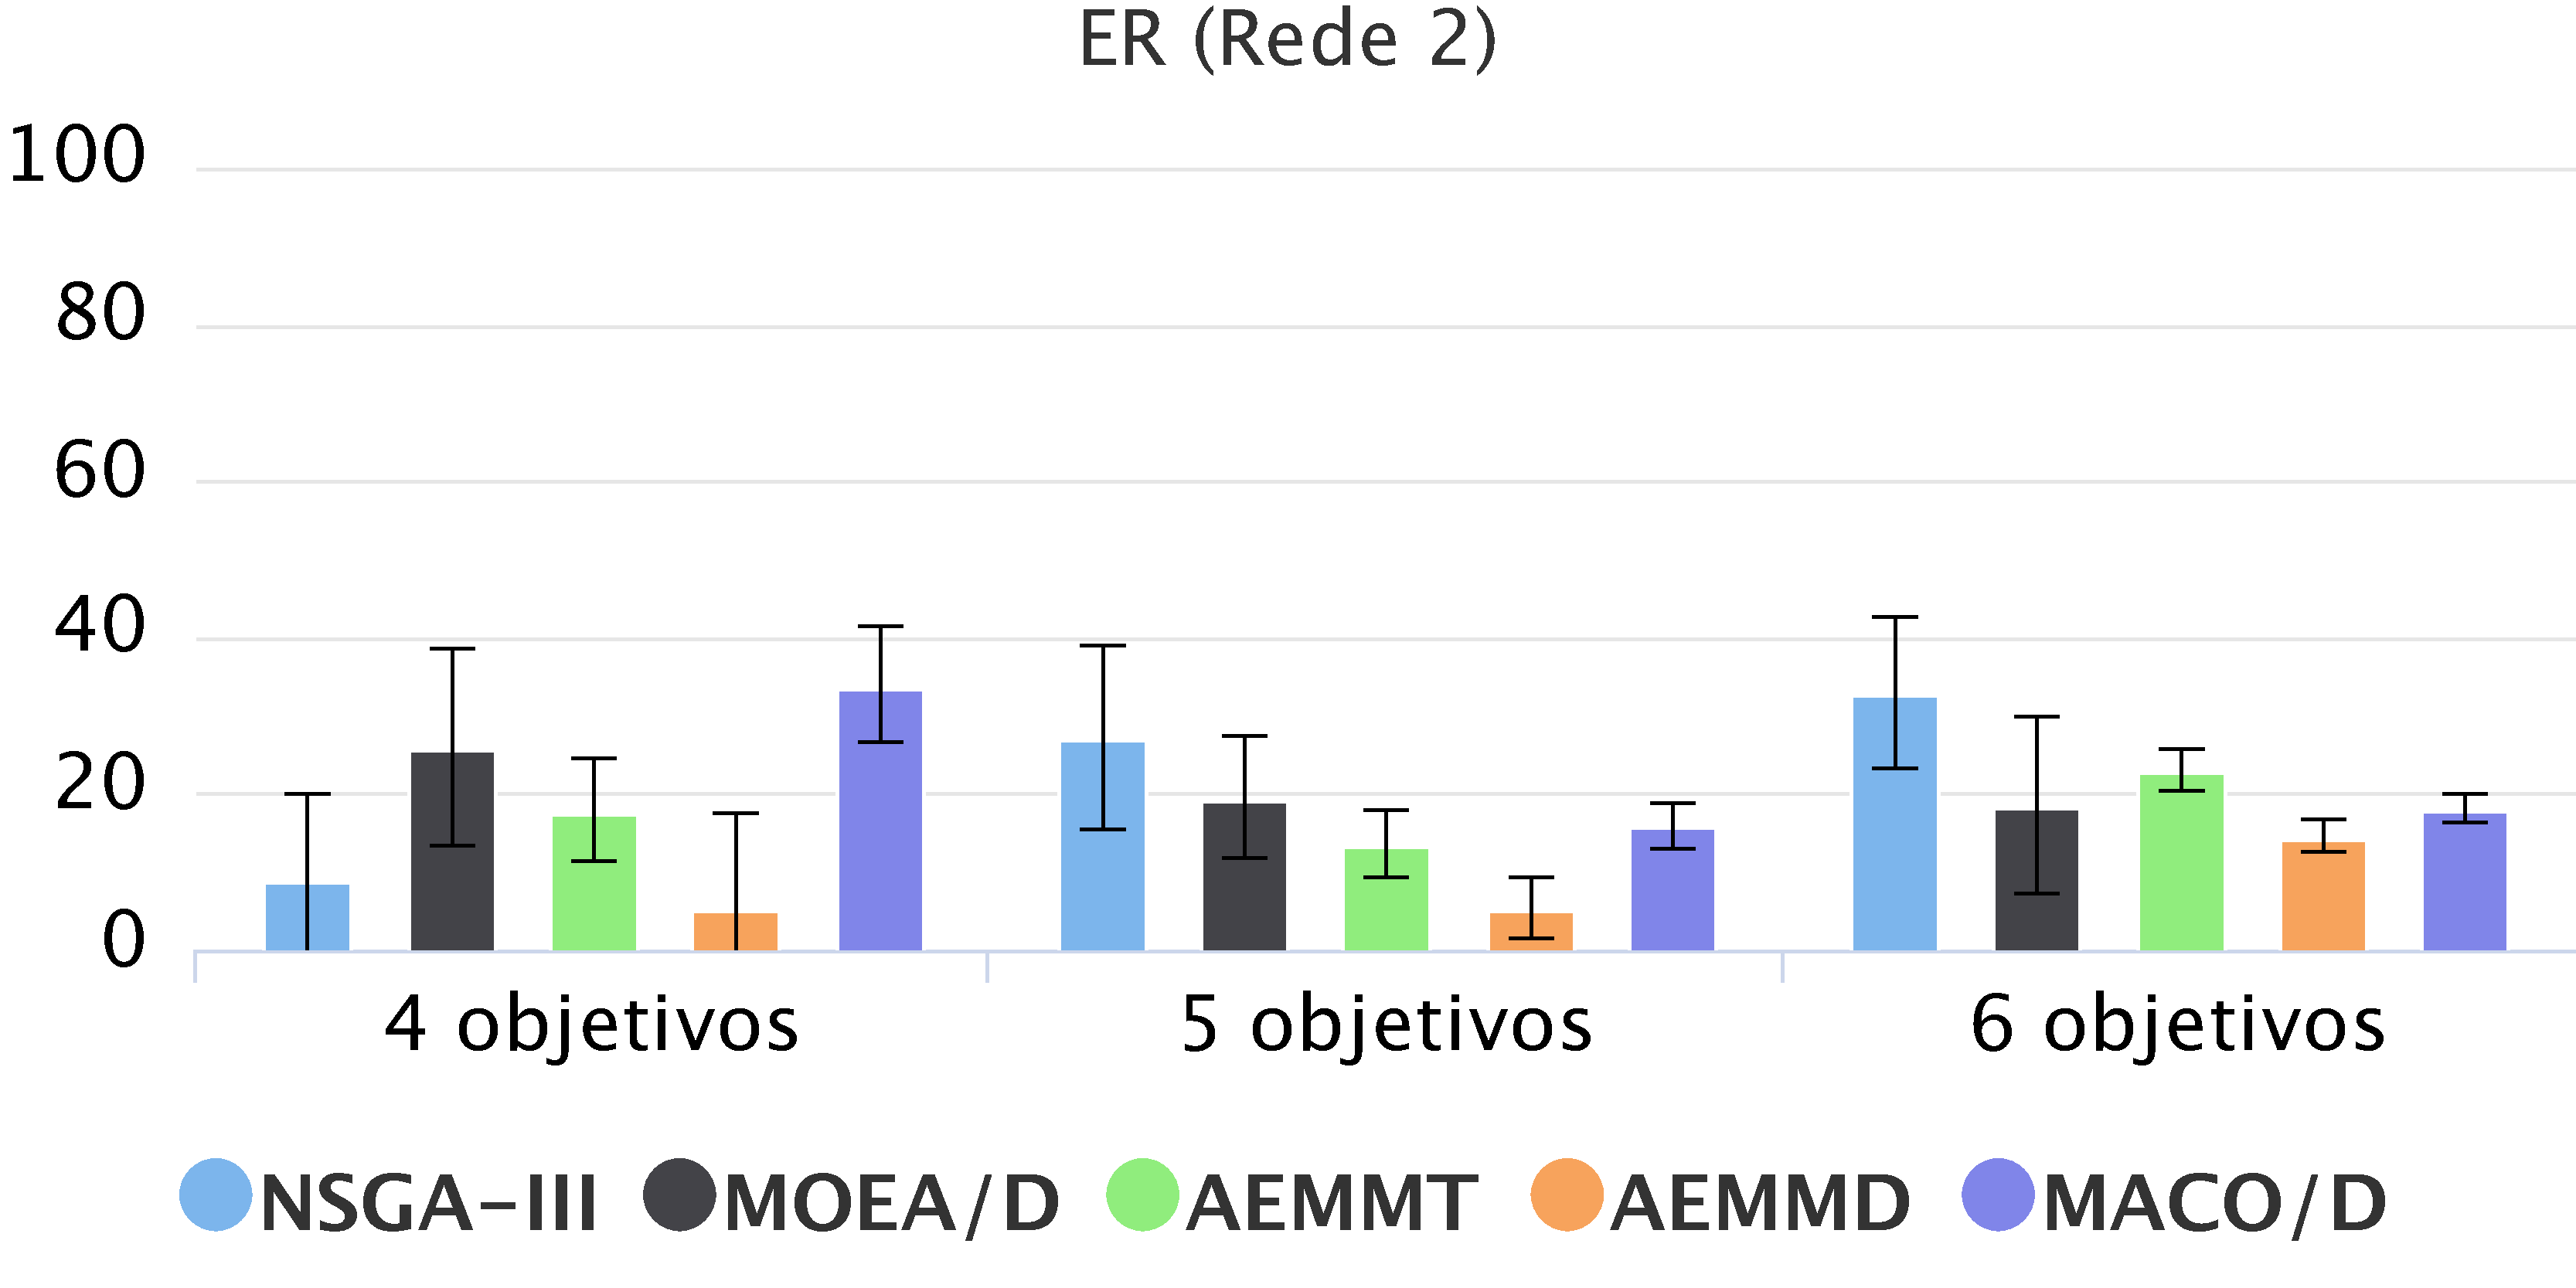
\includegraphics[width=0.5\textwidth]{cap_experimentos/figs/etapa3/er-mrp-r2}
	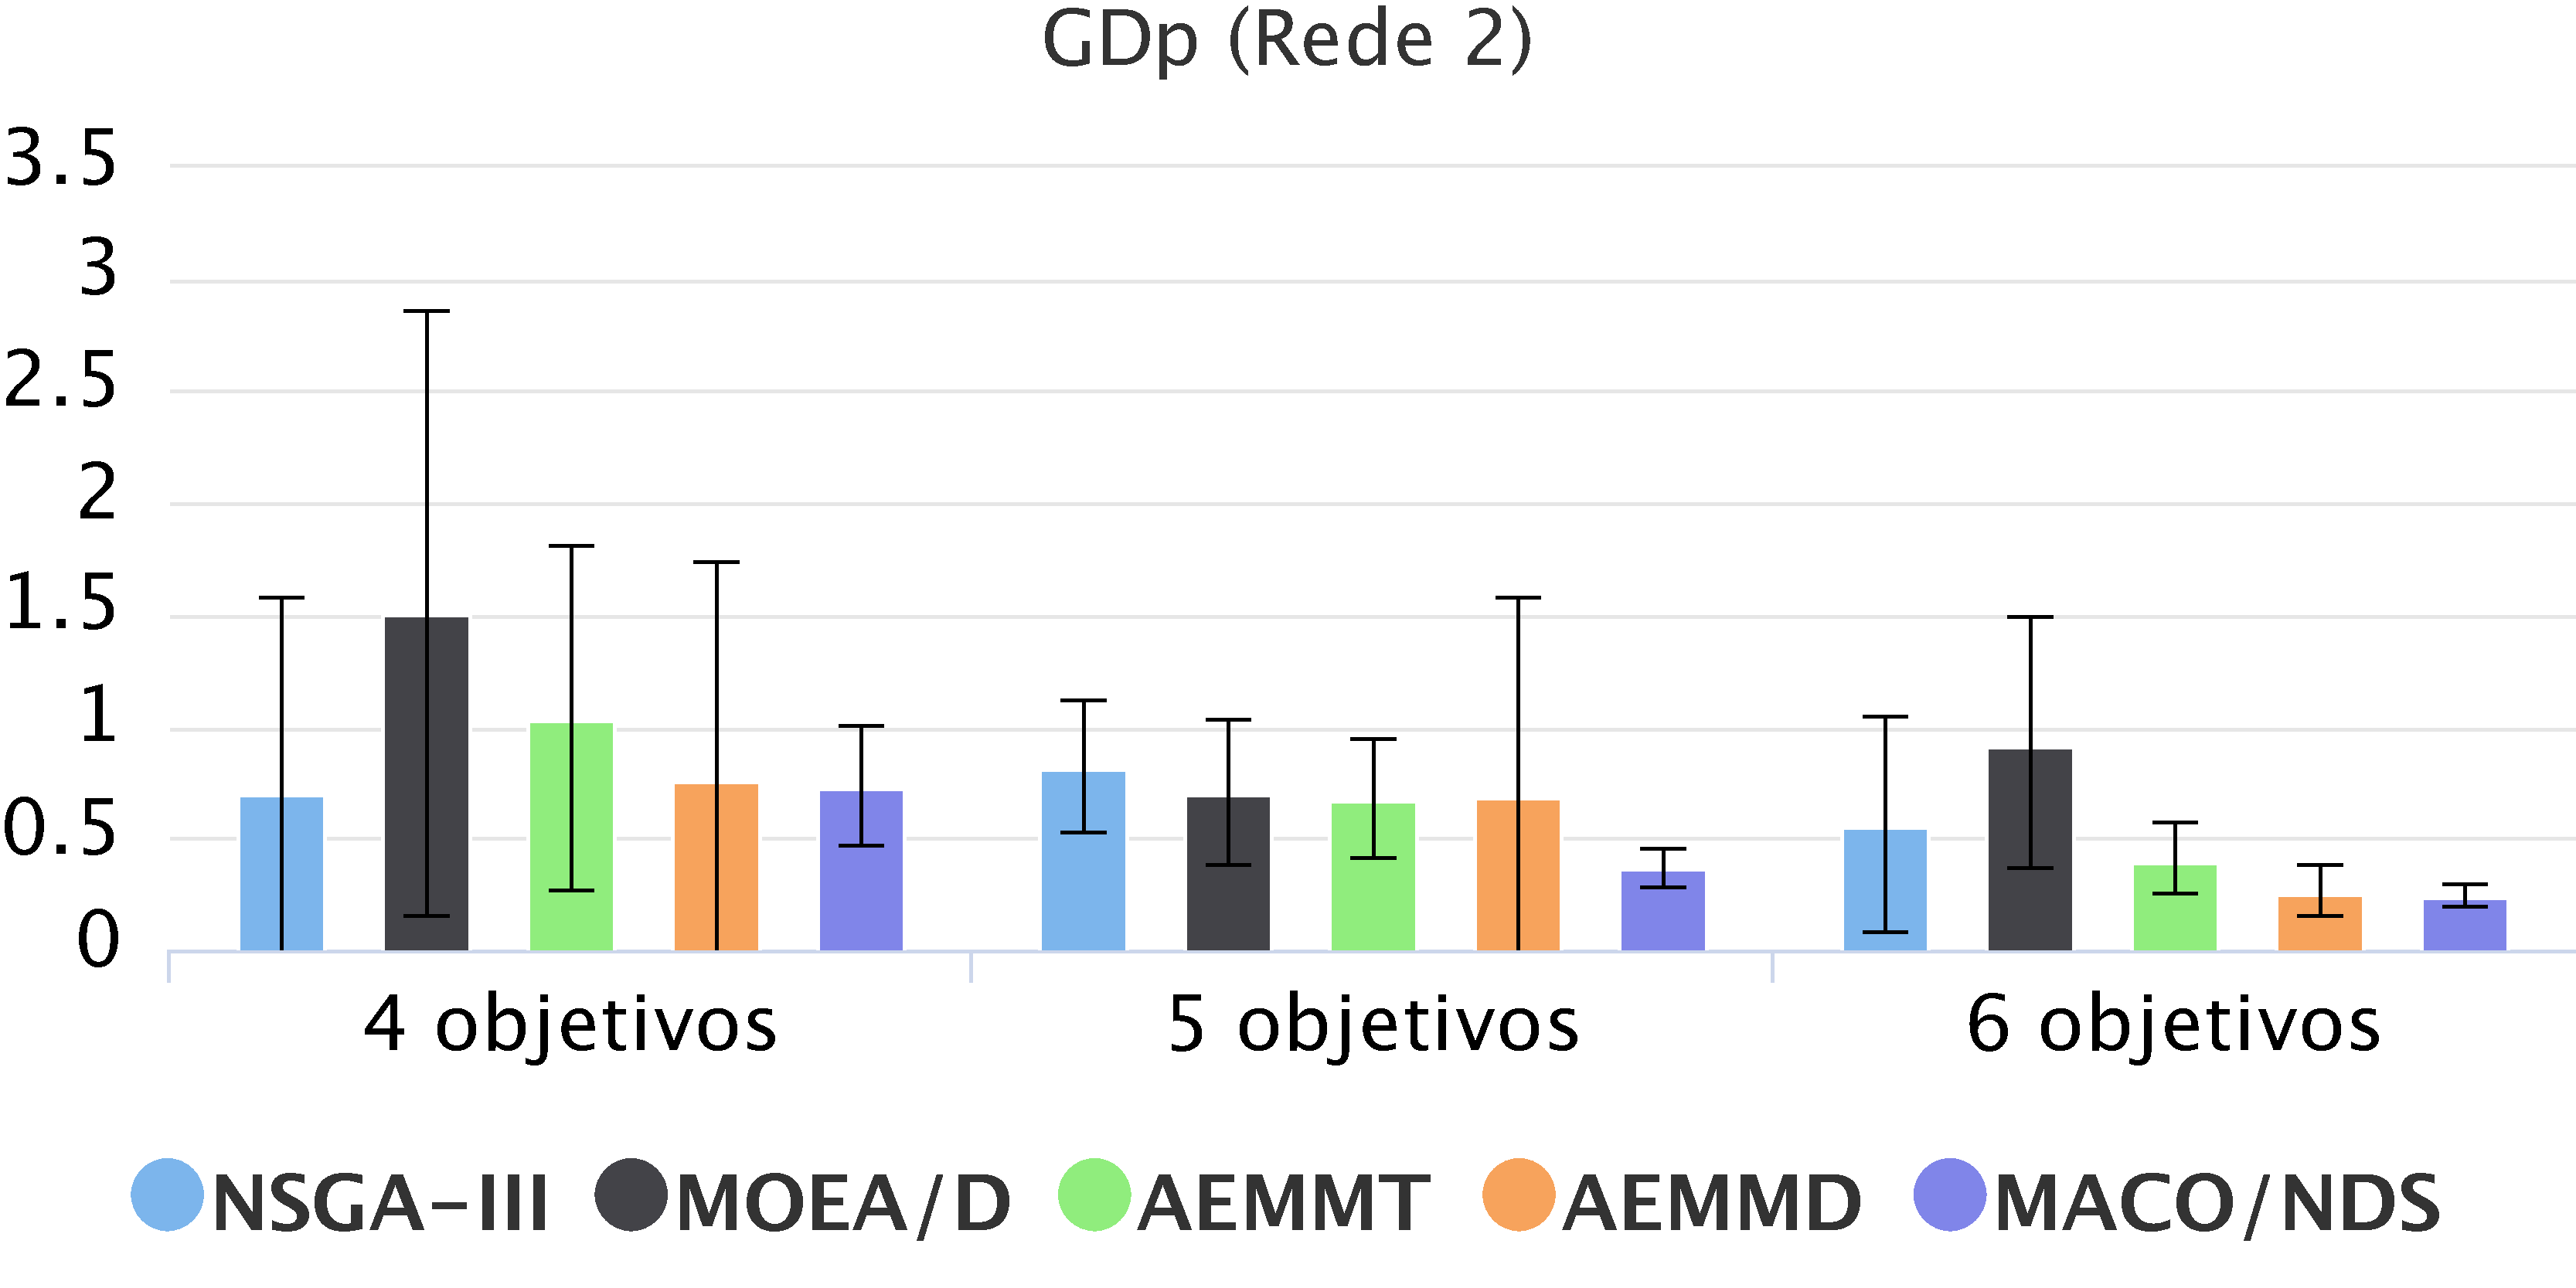
\includegraphics[width=0.5\textwidth]{cap_experimentos/figs/etapa3/gd-mrp-r2}
	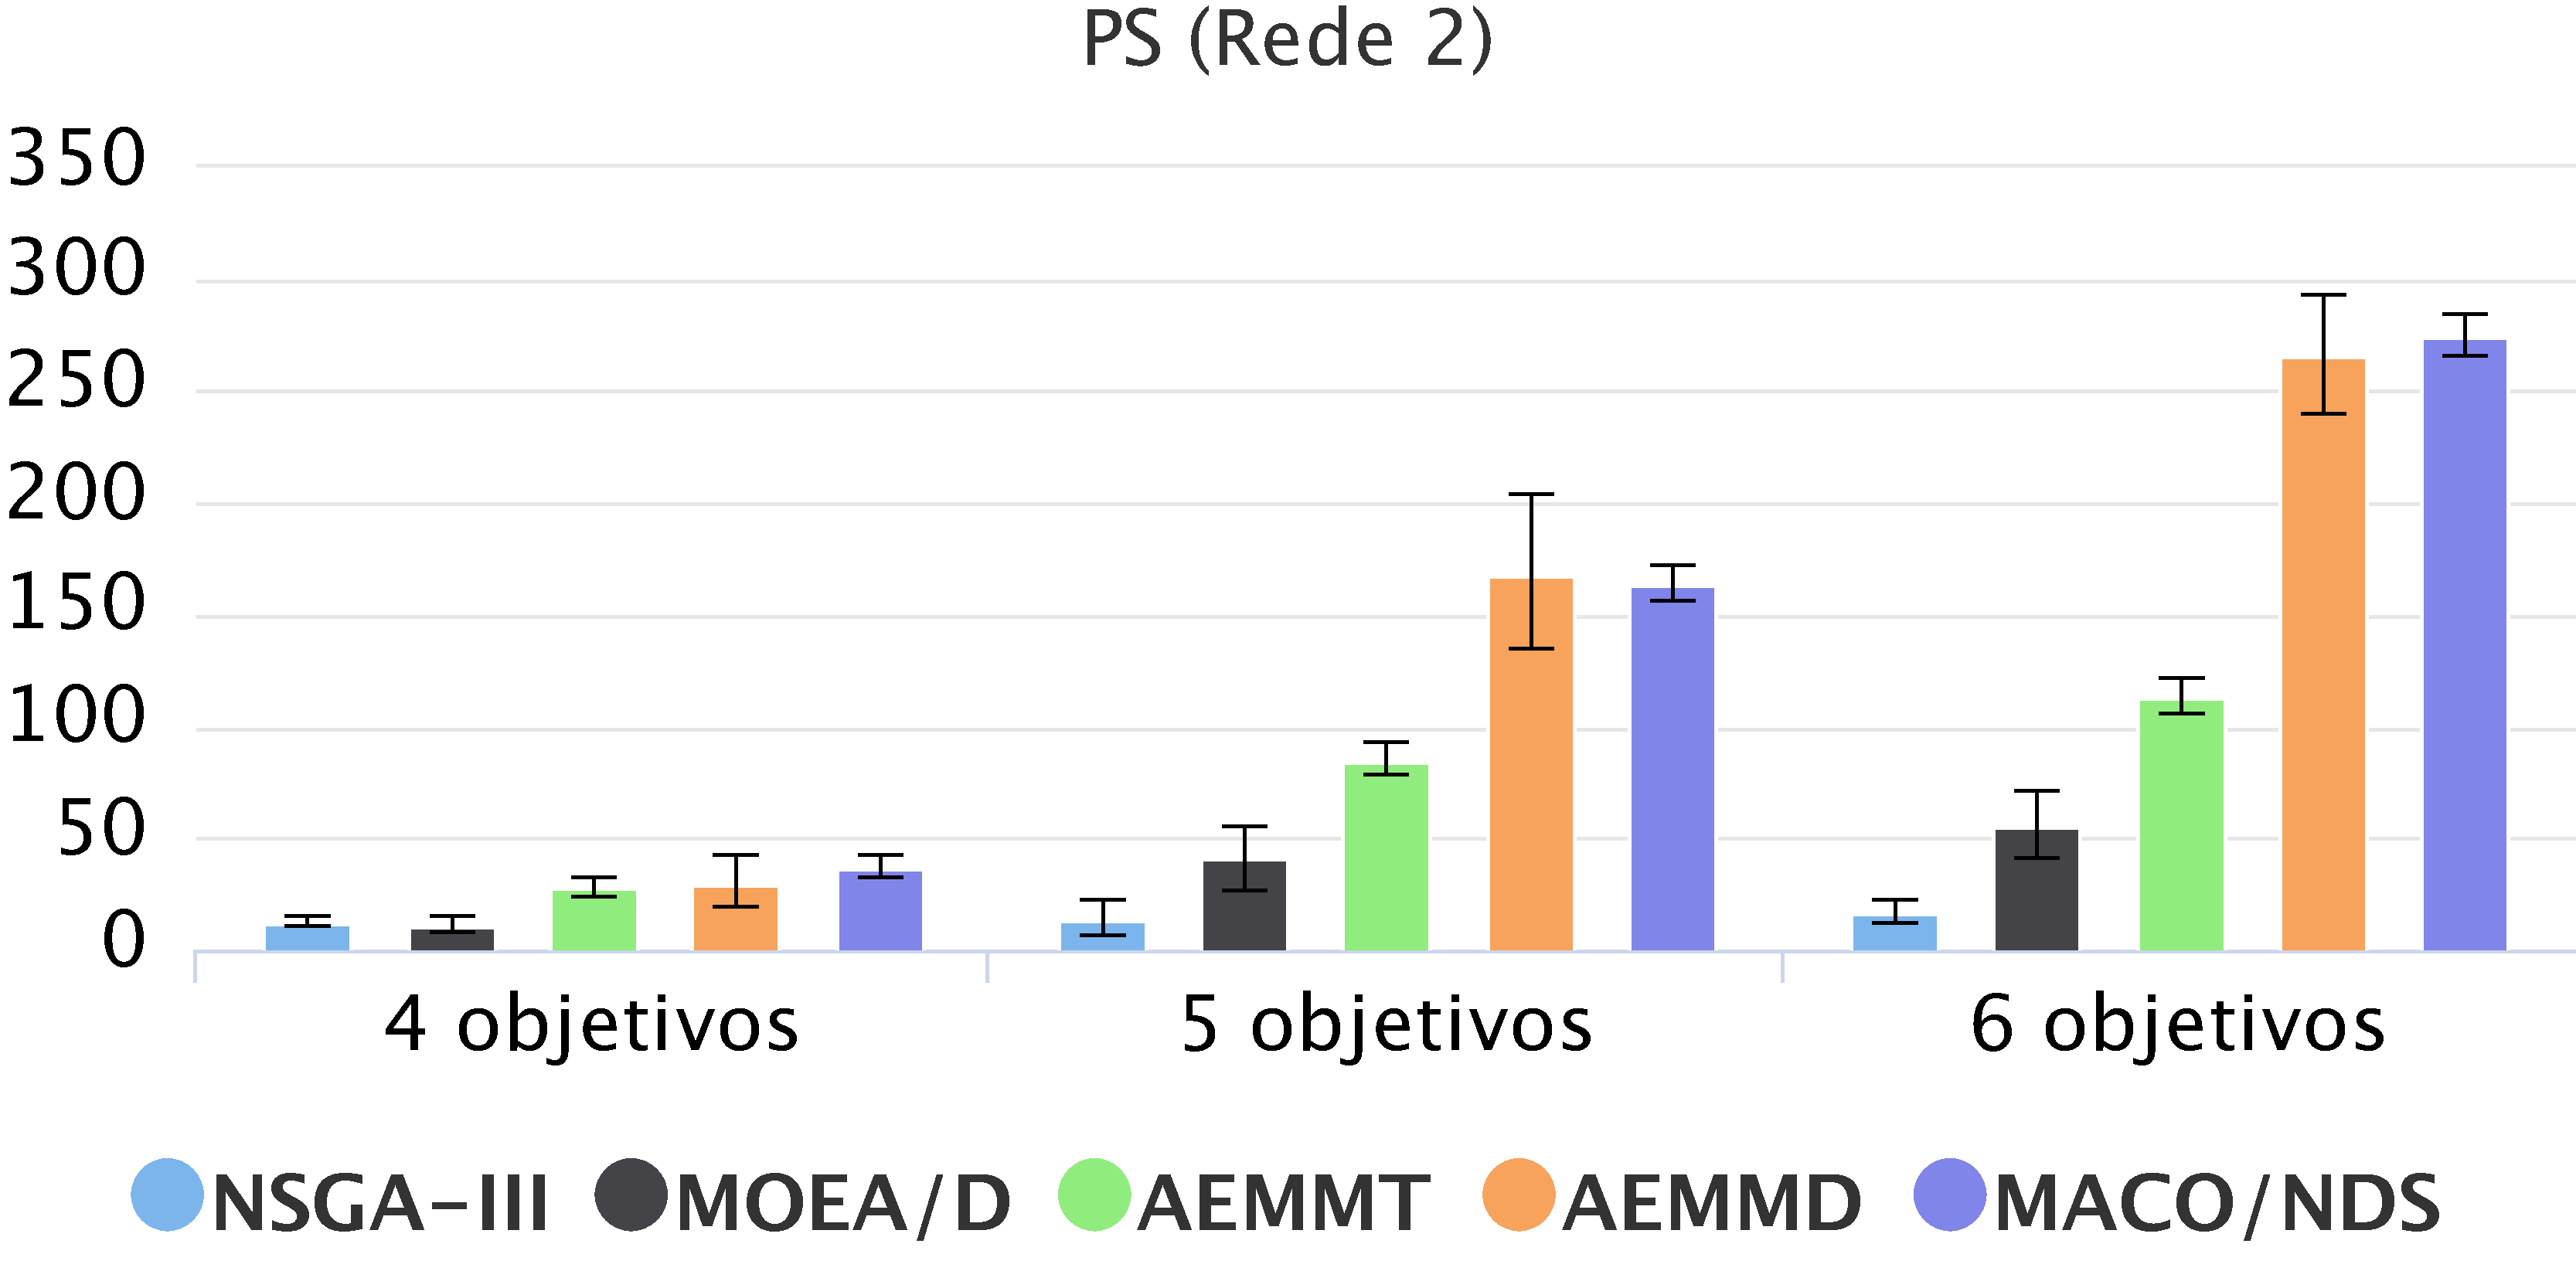
\includegraphics[width=0.5\textwidth]{cap_experimentos/figs/etapa3/ps-mrp-r2}
	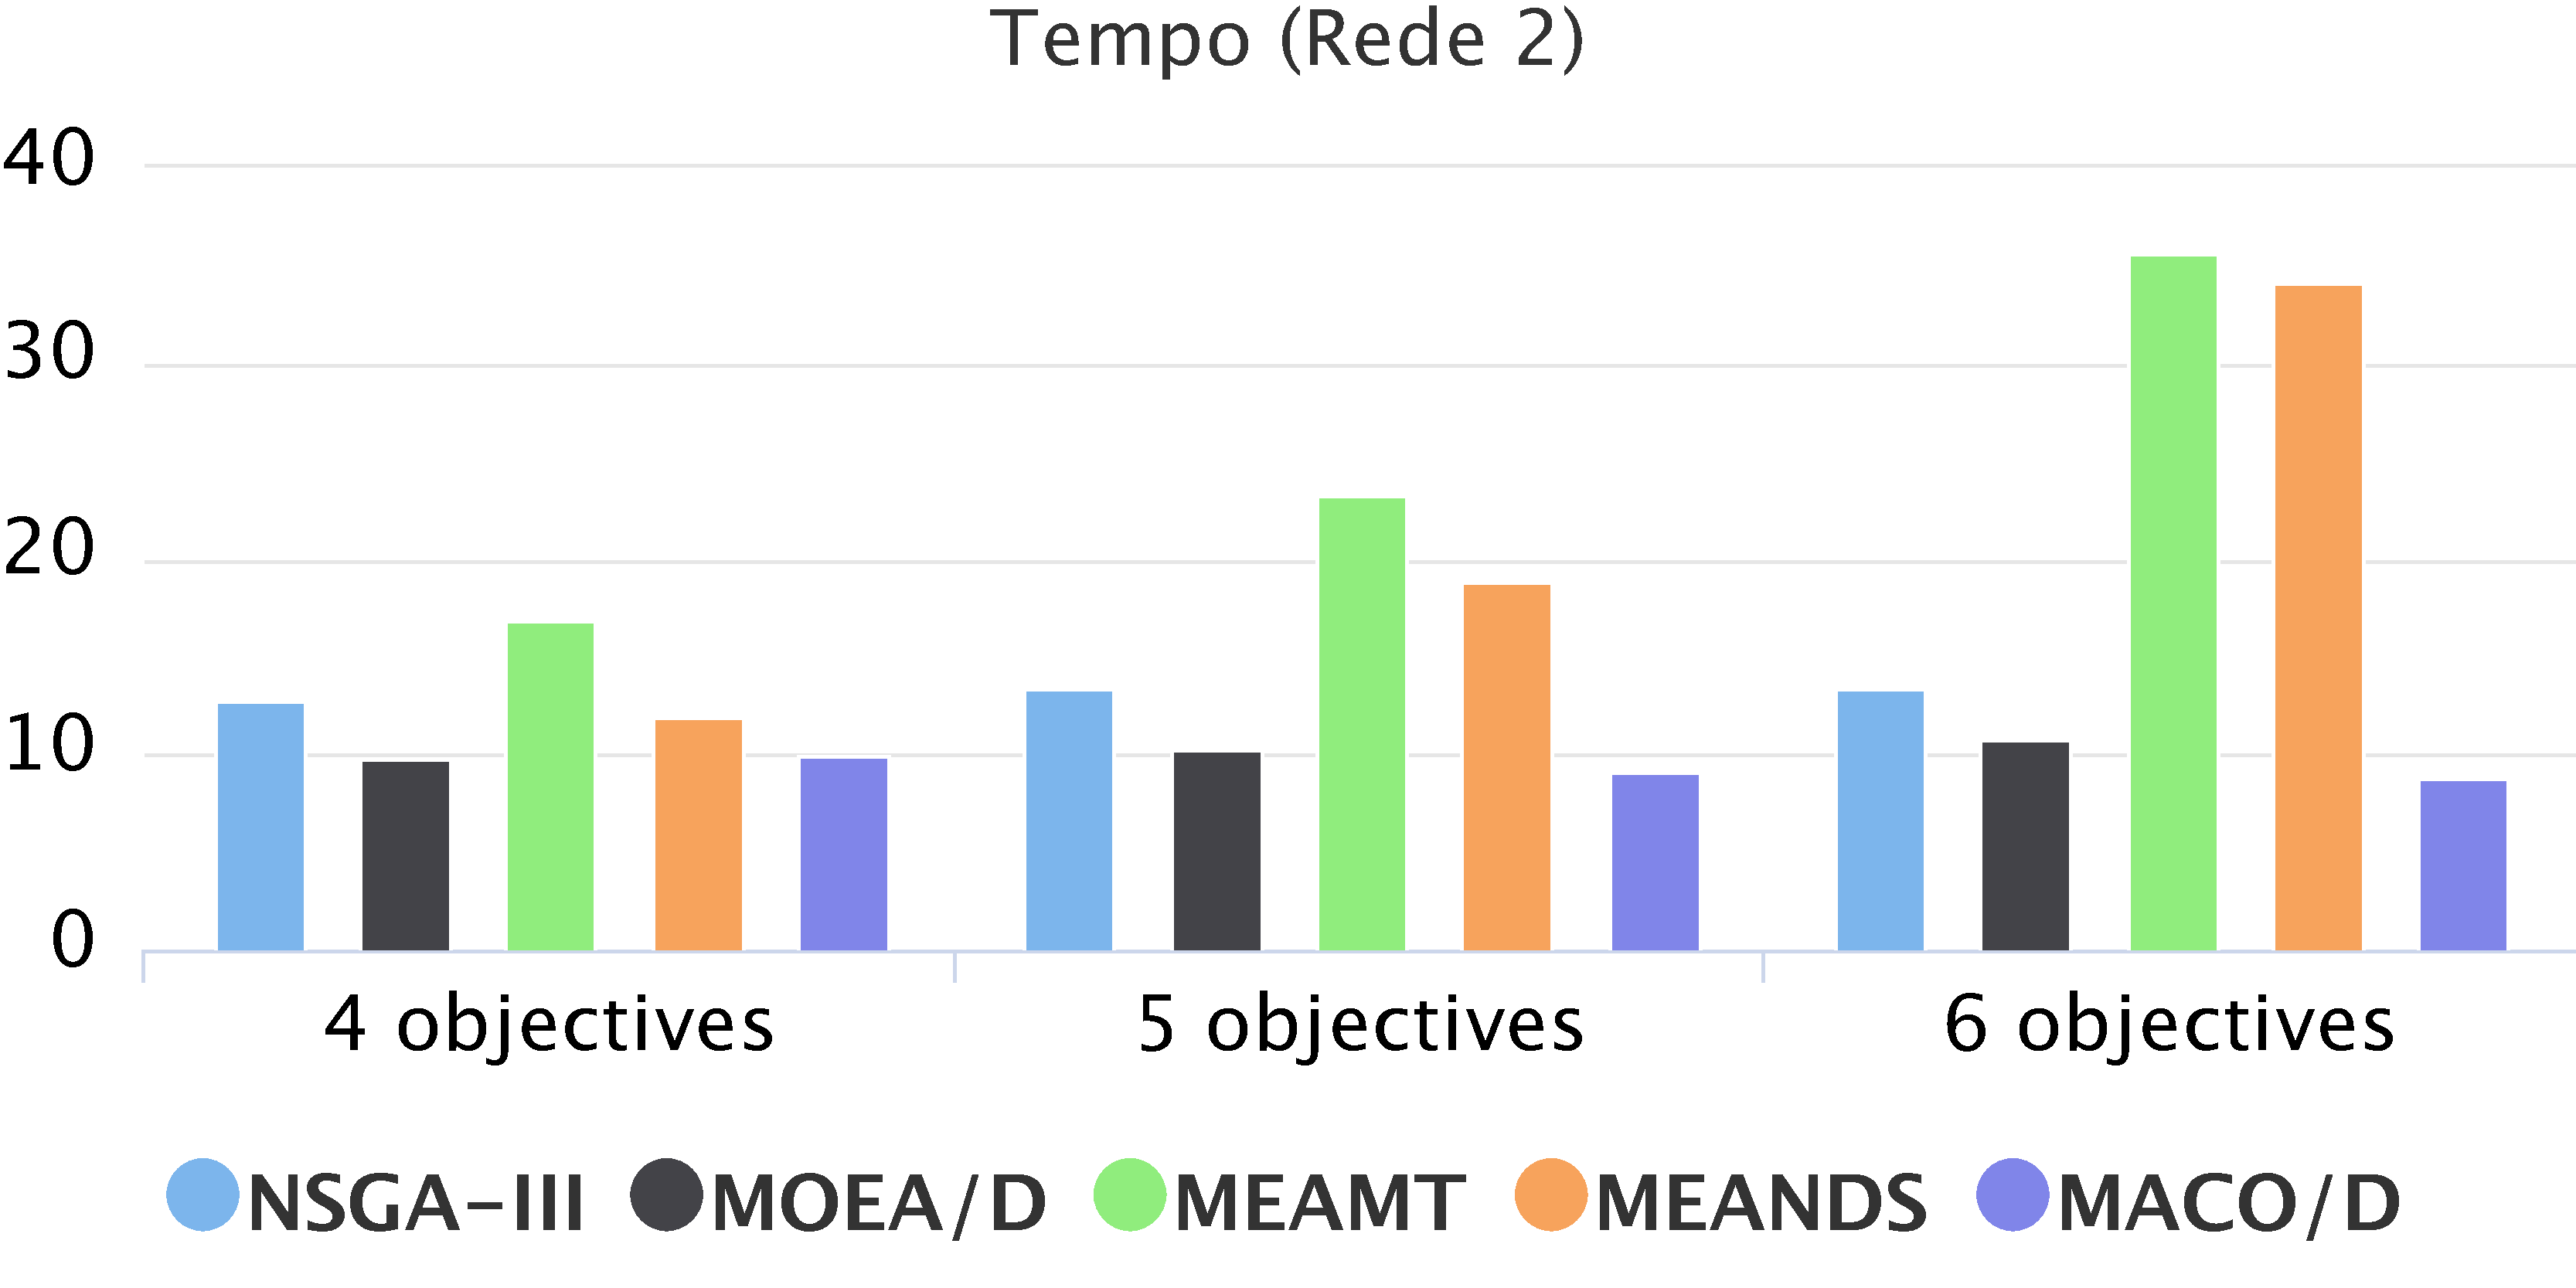
\includegraphics[width=0.5\textwidth]{cap_experimentos/figs/etapa3/time-mrp-r2}
	\caption{\label{fig_exp3_prm_r2}Desempenho dos algoritmos na 3ª etapa para o PRM na rede 2}
\end{figure*}

A \autoref{fig_exp3_prm_r2} apresenta os resultados obtidos pelos algoritmos para a rede 2. Apesar de mais complexa, os gráficos apresentam um comportamento similar ao da instância anterior (rede 1). O AEMMD obtém as menores taxas de erro, seguido pelo AEMMT. O MACO/NDS é o algoritmo que alcança os menores valores para a métrica $GDp$, sendo seguido de perto pelo AEMMT e pelo AEMMD. Considerando a métrica $PS$, os melhores valores foram encontrados pelo AEMMD, mas com uma diferença muito pequena em relação ao MACO/NDS. Os piores valores de $PS$ são retornados pelo NSGA-III. Tal comportamento é decorrência da limitação do algoritmo quanto ao crescimento do Pareto. Analisando o tempo médio de execução, o método mais rápido é o MOEA/D e o mais lento é o AEMMT.

\begin{figure*}[!htbp]
	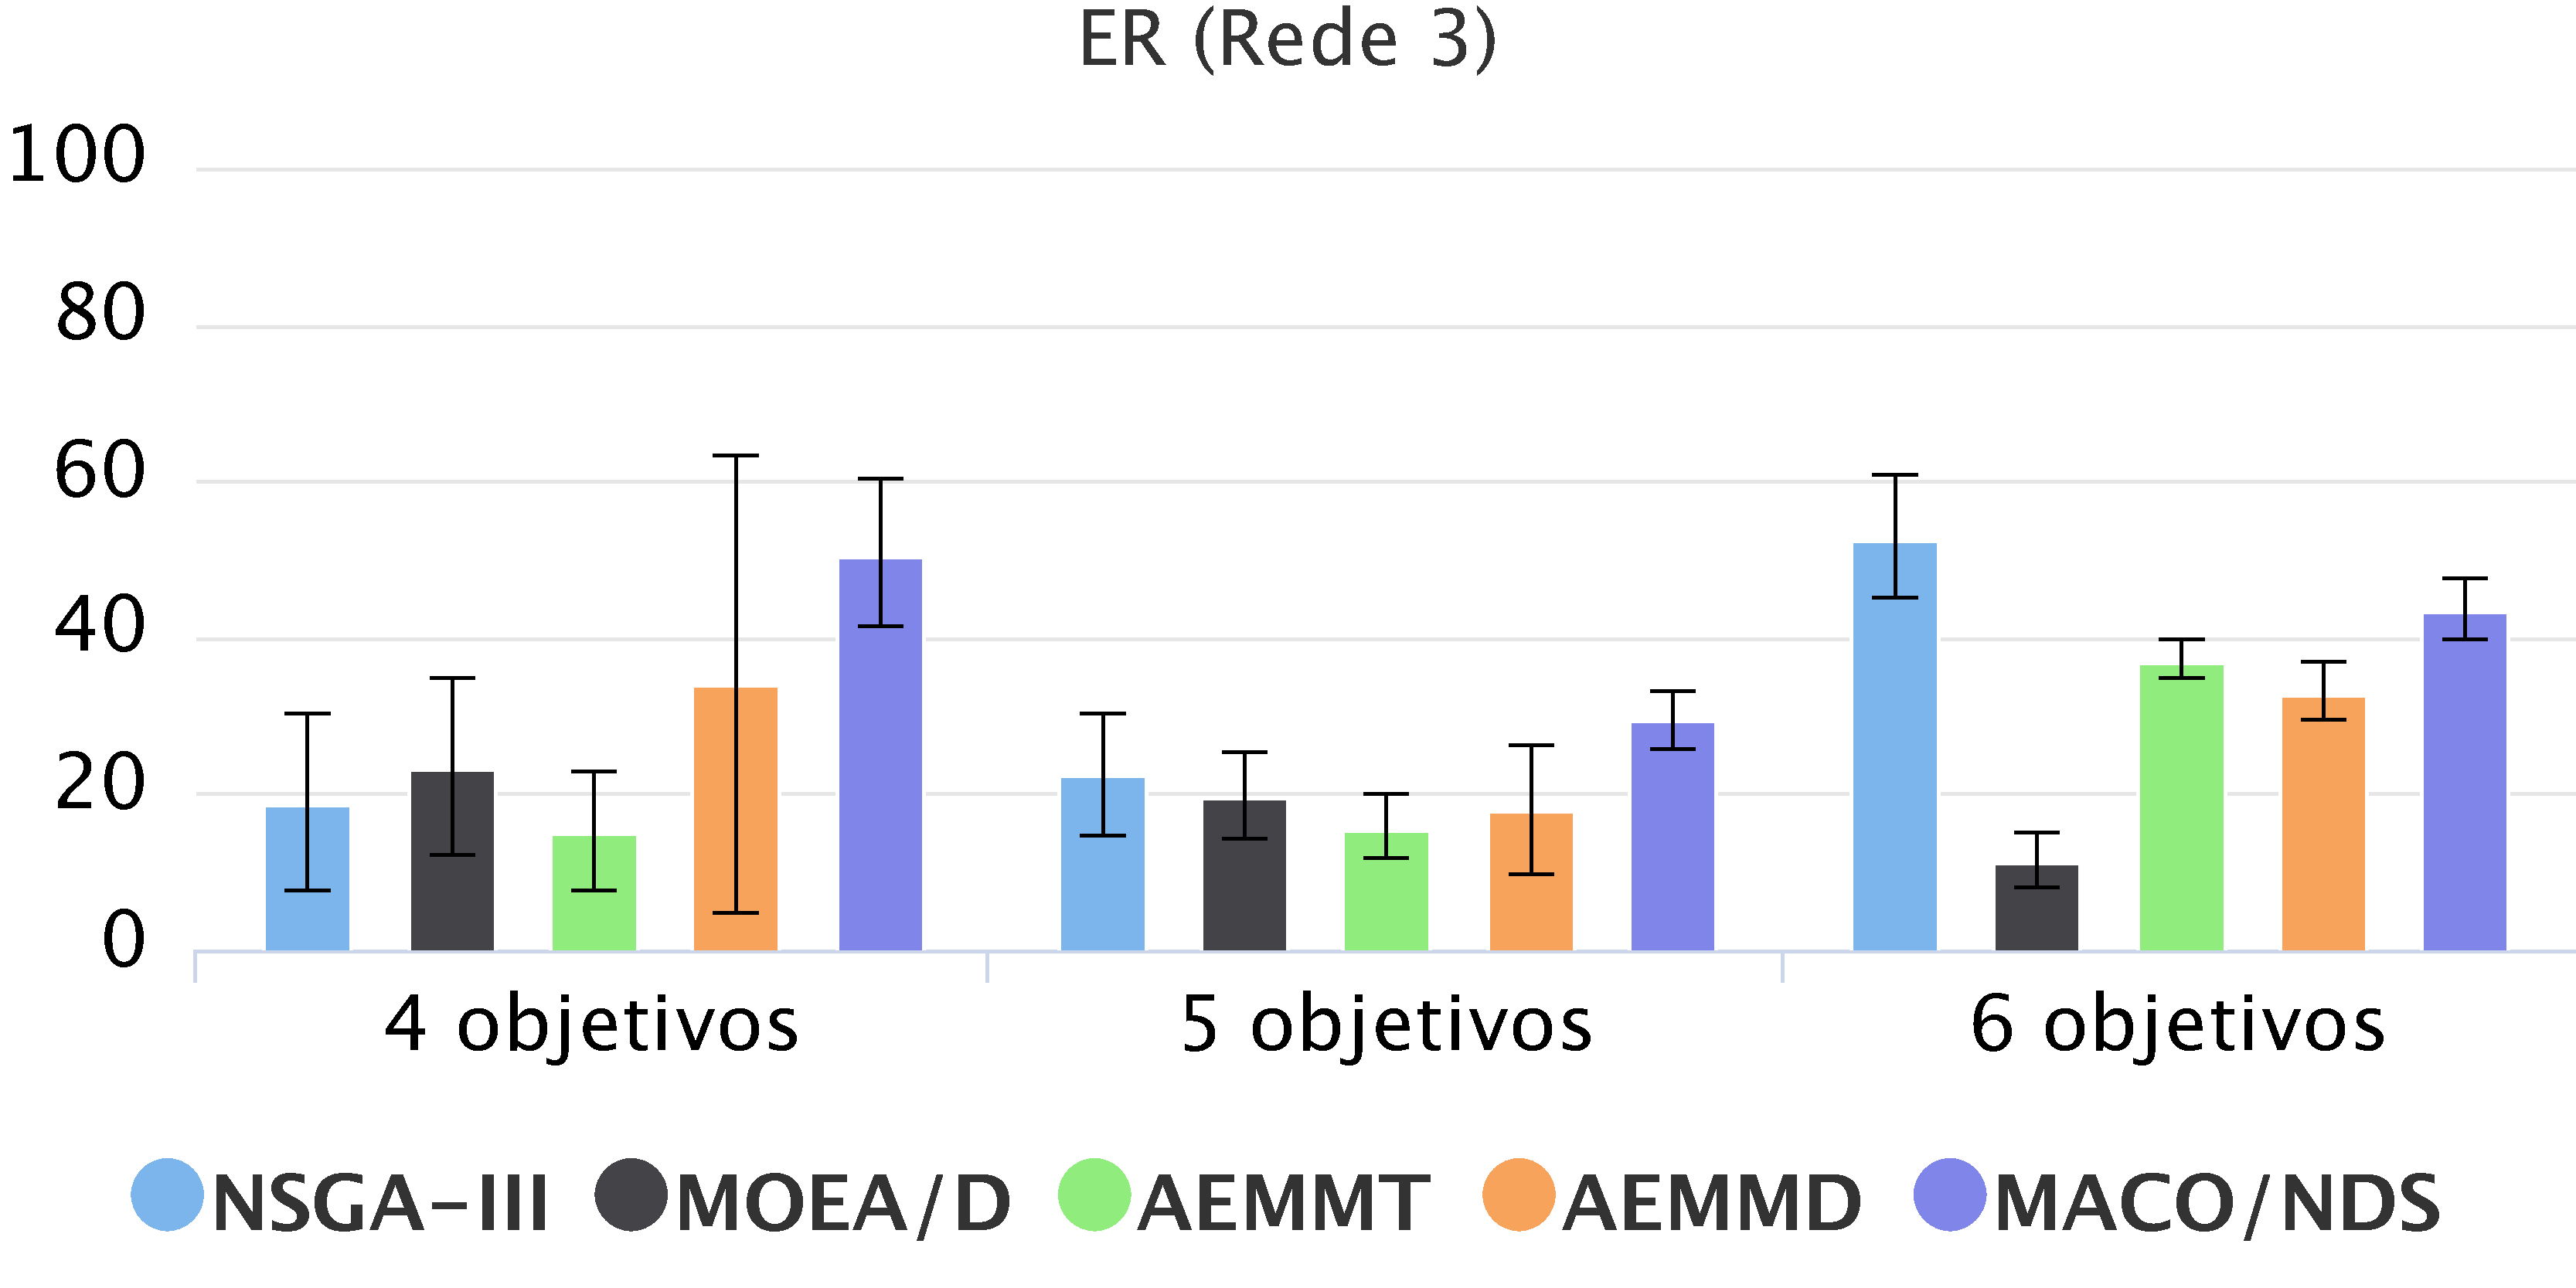
\includegraphics[width=0.5\textwidth]{cap_experimentos/figs/etapa3/er-mrp-r3}
	\includegraphics[width=0.5\textwidth]{cap_experimentos/figs/etapa3/gd-mrp-r3}
	\includegraphics[width=0.5\textwidth]{cap_experimentos/figs/etapa3/ps-mrp-r3}
	\includegraphics[width=0.5\textwidth]{cap_experimentos/figs/etapa3/time-mrp-r3}
	\caption{\label{fig_exp3_prm_r3}Desempenho dos algoritmos na 3ª etapa para o PRM na rede 3}
\end{figure*}

A \autoref{fig_exp3_prm_r3} apresenta o desempenho dos algoritmos no PRM considerando a rede 3, o AEMMT encontra as melhores taxas de erro para 4 (15,2\%) e 5 (15,7\%) objetivos, enquanto que o MOEA/D consegue o melhor resultado para 6 objetivos (11,5\%). O NSGA-III produz o segundo menor $ER$ no problema de 4 objetivos (18,9\%), mas é o segundo pior para 5 objetivos (22,5\%) e o pior com 6 objetivos (52,7\%). O menor $GDp$ no problema com 4 objetivos é dado pelo MACO/NDS (0,7), enquanto o AEMMT obtém os melhores valores nos problemas com 5 e 6 objetivos (0,3 e 0,1, respectivamente). As maiores fronteiras de Pareto são encontradas pelo AEMMD e MACO/NDS, sendo o AEMMD o melhor entre os dois. O algoritmo mais rápido é o MACO/NDS, executando em tempo 5 vezes menor que o método mais lento (AEMMT).

\begin{figure*}[!htbp]	
	\includegraphics[width=0.5\textwidth]{cap_experimentos/figs/etapa3/er-mrp-todos}
	\includegraphics[width=0.5\textwidth]{cap_experimentos/figs/etapa3/gd-mrp-todos}
	\includegraphics[width=0.5\textwidth]{cap_experimentos/figs/etapa3/ps-mrp-todos}
	\includegraphics[width=0.5\textwidth]{cap_experimentos/figs/etapa3/time-mrp-todos}
	\caption{\label{fig_exp3_prm_todos}Resultado consolidado da 3ª etapa considerando o PRM nas redes 1, 2 e 3}
\end{figure*}

Para analisar de forma conjunta os resultados das três redes, todos os experimentos são consolidados através da média aritmética das métricas de desempenho avaliadas. Esses resultados consolidados são apresentados na \autoref{fig_exp3_prm_todos}. De maneira geral, o NSGA-III consegue soluções de qualidade razoável, mas apresenta baixo $PS$ e um tempo de execução mediano. O MOEA/D obtém as melhores taxas de erro no problema de seis objetivos, mas tem um desempenho modesto nos problemas de 4 e 5 objetivos. O algoritmo também está entre os piores para as métricas $GDp$ e $PS$. A velocidade de execução do MOEA/D é tão boa quanto a do MACO/NDS, sendo os dois algoritmos mais rápidos. Assim, o uso desse algoritmo pode ser uma boa opção quando o objetivo da busca é conseguir uma baixa taxa de erro em uma execução mais rápida, sem se preocupar com o $PS$. Analisando-se todas as métricas, os melhores resultados foram obtidos pelo AEMMD e o algoritmo proposto (MACO/NDS). Com relação ao erro, o AEMMD consegue as melhores taxas, enquanto o MACO/NDS, juntamente com o NSGA-III, apresentam os piores valores. Analisando-se o $GDp$, existe uma pequena diferença entre os algoritmos, mas o MACO/NDS gera melhores soluções que o AEMMD. Além disso, o desvio padrão do MACO/NDS é significativamente menor, tornando-o um método mais estável quanto à qualidade das soluções. Um desempenho similar também é observado para a métrica PS. Entretanto, nesse caso, o AEMMD produz as maiores fronteiras de Pareto que o MACO/NDS. Por outro lado, ao analisar o tempo médio de execução, observa-se que o MACO/NDS é consideravelmente mais rápido, chegando a executar em quase 5 vezes menos tempo. Considerando que o PRM é um problema sensível ao tempo de execução, apesar do AEMMD obter um desempenho razoavelmente superior nas métricas $ER$ e $PS$, o MACO/NDS é a melhor opção entre os algoritmos testados, pelo menos nos cenários analisados.

A principal diferença no desempenho do algoritmo proposto (MACO/NDS) em relação aos dois problemas investigados (PMM e PRM) é o tempo de execução. Considerando-se os resultados do PMM apresentados na \autoref{fig_exp3_pmm_todos}, o MACO/NDS é o segundo algoritmo mais lento e seu tempo de execução está altamente relacionado ao número de objetivos. Na \autoref{fig_exp3_prm_todos}, que representa o comportamento geral dos algoritmos no PRM, observa-se o oposto, ou seja, o MACO/NDS é o algoritmo mais rápido e seu tempo de execução se mantém estável, independentemente da formulação de objetivos. Concluímos que essa diferença de comportamento é decorrência do tamanho da fronteira de Pareto (soluções não dominadas). O processo de maior custo computacional no MACO/NDS é a atualização dos feromônios, onde é necessário recalcular o conjunto de soluções não-dominadas $nd$. A cada iteração, para toda solução criada, é necessário passar por todos elementos em $nd$ verificando a relação de não-dominância. Naturalmente, quanto maior o conjunto $nd$, mais caro se torna o processo. No PRM, foram encontradas fronteiras de Pareto de tamanho razoavelmente pequenos, todas com menos de 350 elementos. Nesse caso, para cada solução criada, é preciso fazer no máximo 350 comparações. No PMM, as fronteiras de Pareto são muito grandes. Por exemplo, no problema com 6 objetivos e 50 itens, a cardinalidade do conjunto $nd$ chega a ser maior que 4500 soluções. Quanto maior a quantidade de objetivos do problema, maior o número de soluções no Pareto e mais lento será a classificação de soluções não dominadas. Se o conjunto $nd$ é pequeno até mesmo para a maior quantidade de objetivos (caso do PRM), o processo será rápido e o tempo de execução não será muito diferente entre as formulações de objetivos. Por outro lado, se a cardinalidade de $nd$ é grande e cresce consideravelmente com o aumento na quantidade de objetivos, o tempo necessário para se atualizar os feromônios será muito alto e apresentará grande variação conforme a formulação de objetivos.

A fim de melhor comparar o MACO/NDS aos algoritmos AEMMT e AEMMD, realizou-se o teste de hipótese Z (\textit{Z-test}) com 5\% de significância ($\alpha=0,05$), sendo os resultados mostrados nas Tabelas \ref{tab_ztest_meamt} e \ref{tab_ztest_meams}, respectivamente. Em ambas as tabelas, uma célula de fundo verde representa um cenário onde o MACO/NDS obteve melhor resultado que seu adversário, vermelho significa que o adversário foi melhor e a célula branca indica empate.

\begin{table}[htb]
	\centering
	\def\arraystretch{1.0}
	\caption{Testes de hipótese entre o MACO/NDS e o AEMMT para os problemas investigados}
	\label{tab_ztest_meamt}
	\begin{tabular}{cccccccccc}
		& \multicolumn{3}{l}{\textbf{4 objectives}} & \multicolumn{3}{l}{\textbf{5 objectives}} & \multicolumn{3}{l}{\textbf{6 objectives
		}} \\
		\textbf{Instance} & \textbf{ER} & \textbf{GDp} & \textbf{PS} & \textbf{ER} & \textbf{GDp} & \textbf{PS} & \textbf{ER} & \textbf{GDp} & \textbf{PS} \\ \hline
		30 items & \cellcolor{white} $=$ & \cellcolor{table-green} $<$ & \cellcolor{table-green} $>$ & \cellcolor{table-red} $>$ & \cellcolor{table-green} $<$ & \cellcolor{table-green} $>$ & \cellcolor{table-red} $>$ & \cellcolor{table-green} $<$ & \cellcolor{table-green} $>$ \\
		40 items & \cellcolor{table-green} $<$ & \cellcolor{table-green} $<$ & \cellcolor{table-green} $>$ & \cellcolor{table-green} $<$ & \cellcolor{table-green} $<$ & \cellcolor{table-green} $>$ & \cellcolor{table-red} $>$ & \cellcolor{table-green} $<$ & \cellcolor{table-green} $>$ \\
		50 items & \cellcolor{table-green} $<$ & \cellcolor{white} $=$ & \cellcolor{table-green} $>$ & \cellcolor{table-green} $<$ & \cellcolor{table-green} $<$ & \cellcolor{table-green} $>$ & \cellcolor{table-red} $>$ & \cellcolor{table-green} $<$ & \cellcolor{table-green} $>$ \\  \hline 
		Rede 1 & \cellcolor{table-red} $>$ & \cellcolor{table-green} $<$ & \cellcolor{table-red} $<$ & \cellcolor{table-red} $>$ & \cellcolor{table-green} $<$ & \cellcolor{table-green} $>$ & \cellcolor{table-red} $>$ & \cellcolor{table-green} $<$ & \cellcolor{table-green} $>$ \\
		Rede 2 & \cellcolor{table-red} $>$ & \cellcolor{table-green} $<$ & \cellcolor{table-green} $>$ & \cellcolor{table-red} $>$ & \cellcolor{table-green} $<$ & \cellcolor{table-green} $>$ & \cellcolor{table-green} $<$ & \cellcolor{table-green} $<$ & \cellcolor{table-green} $>$ \\
		Rede 3 & \cellcolor{table-red} $>$ & \cellcolor{table-green} $<$ & \cellcolor{table-red} $<$ & \cellcolor{table-red} $>$ & \cellcolor{table-green} $<$ & \cellcolor{table-green} $>$ & \cellcolor{table-red} $>$ & \cellcolor{table-red} $>$ & \cellcolor{table-green} $>$ \\  \hline 
	\end{tabular}
\end{table}

\begin{table}[htb]
	\centering
	\def\arraystretch{1.0}
	\caption{Testes de hipótese entre o MACO/NDS e o AEMMD para os problemas investigados}
	\label{tab_ztest_meams}
	\begin{tabular}{cccccccccc}
		& \multicolumn{3}{l}{\textbf{4 objectives}} & \multicolumn{3}{l}{\textbf{5 objectives}} & \multicolumn{3}{l}{\textbf{6 objectives
		}} \\
		\textbf{Instance} & \textbf{ER} & \textbf{GDp} & \textbf{PS} & \textbf{ER} & \textbf{GDp} & \textbf{PS} & \textbf{ER} & \textbf{GDp} & \textbf{PS} \\ \hline
		30 items & \cellcolor{table-green} $<$ & \cellcolor{table-green} $<$ & \cellcolor{table-green} $>$ & \cellcolor{table-green} $<$ & \cellcolor{table-red} $>$ & \cellcolor{table-green} $>$ & \cellcolor{table-green} $<$ & \cellcolor{table-red} $>$ & \cellcolor{table-green} $>$ \\
		40 items & \cellcolor{table-green} $<$ & \cellcolor{table-red} $>$ & \cellcolor{table-green} $>$ & \cellcolor{table-green} $<$ & \cellcolor{table-red} $>$ & \cellcolor{table-green} $>$ & \cellcolor{table-green} $<$ & \cellcolor{table-red} $>$ & \cellcolor{table-green} $>$ \\
		50 items & \cellcolor{table-green} $<$ & \cellcolor{table-green} $<$ & \cellcolor{table-green} $>$ & \cellcolor{table-green} $<$ & \cellcolor{table-green} $<$ & \cellcolor{table-green} $>$ & \cellcolor{table-green} $<$ & \cellcolor{table-green} $<$ & \cellcolor{table-green} $>$ \\  \hline 
		Rede 1 & \cellcolor{table-red} $>$ & \cellcolor{table-green} $<$ & \cellcolor{table-red} $<$ & \cellcolor{table-red} $>$ & \cellcolor{table-green} $<$ & \cellcolor{table-red} $<$ & \cellcolor{table-red} $>$ & \cellcolor{table-green} $<$ & \cellcolor{table-red} $<$ \\
		Rede 2 & \cellcolor{table-red} $>$ & \cellcolor{white} $=$ & \cellcolor{table-green} $>$ & \cellcolor{table-red} $>$ & \cellcolor{table-green} $<$ & \cellcolor{table-red} $<$ & \cellcolor{table-red} $>$ & \cellcolor{table-green} $<$ & \cellcolor{table-green} $>$ \\
		Rede 3 & \cellcolor{table-red} $>$ & \cellcolor{table-green} $<$ & \cellcolor{table-red} $<$ & \cellcolor{table-red} $>$ & \cellcolor{white} $=$ & \cellcolor{table-red} $<$ & \cellcolor{table-red} $>$ & \cellcolor{table-red} $>$ & \cellcolor{table-red} $<$ \\  \hline 
	\end{tabular}
\end{table}

Analisando-se o comportamento dos algoritmos, a partir da Tabela \ref{tab_ztest_meamt}, é possível confirmar a superioridade do MACO/NDS em relação ao AEMMT na maioria dos cenários, em ambos os problemas. Na comparação entre o MACO/NDS e o AEMMD, apresentados na Tabela \ref{tab_ztest_meams}, o algoritmo baseado em formigas foi melhor no PMM, mas pior no PRM. Entretanto, o teste de hipótese não considera o tempo de execução, no qual o MACO/NDS foi muito superior ao AEMMD, o que pode ser observado pela \autoref{fig_exp3_prm_todos}.

No PMM, se o tempo de execução é uma preocupação, a melhor alternativa é o algoritmo MOEA/D, que é mais rápido e produz bons resultados. Se a rapidez do algoritmo não é tão importante e deseja-se encontrar um conjunto de soluções mais próximo do Pareto real, o MACO/NDS é o algoritmo mais indicado. No PRM, o método que representa melhor relação entre qualidade e tempo é o MACO/NDS. Por outro lado, se tempo não é importante, o AEMMD é preferível.

A partir desses experimentos, foi publicado um artigo científico no \textit{2018 IEEE Congress on Evolutionary Computation} \cite{Franca2018}.

\section{Análise baseada no hiper-volume}
\label{section_experimentos_etapa4}

Na quarta etapa, os experimentos visam avaliar os algoritmos de otimização \textit{many-objective} NSGA-III, SPEA2-SDE, MOEA/D, AEMMT, AEMMD, MOEA/D-ACO, MOACS e MACO/NDS em instâncias complexas do PMM e PRM utilizando a métrica hiper-volume, a qual independe da estimação e/ou do conhecimento prévio da fronteira de Pareto. Esses experimentos são necessários, pois as etapas anteriores consideraram apenas problemas com complexidade razoável, nos quais é possível estimar previamente a Fronteira de Pareto. Em grande parte dos problemas reais, esse conhecimento prévio é impraticável. Por exemplo, com a inclusão de mais itens no PMM ou o uso de redes mais complexas no PRM torna inviável a obtenção da fronteira de Pareto e se faz necessária a utilização de uma métrica não-paramétrica, neste caso o hiper-volume, para avaliar o desempenho dos algoritmos.

A fim de analisar o comportamento dos algoritmos em espaços de busca mais complexos, duas novas redes (redes 4 e 5), , também investigadas em \cite{LafetaThesis}, e duas novas instâncias do problema da mochila (100 e 200 itens) foram utilizadas. Entretanto, o aumento da complexidade influencia diretamente na cardinalidade do espaço de soluções, tornando inviável a obtenção de um conjunto estável de soluções não-dominadas (fronteira de Pareto aproximada). Tal situação é observada no PRM com as redes $R_3$, $R_4$ e $R_5$, e no PMM com 50, 100 e 200 itens. Nesses cenários, não é adequado basear as conclusões das análises em métricas de desempenho paramétricas, as quais são dependentes do Pareto aproximado. Por isso, nos experimentos dessa etapa, as avaliações consideram apenas duas métricas não-paramétricas, hiper-volume e tempo, as quais são independentes do Pareto.

O hiper-volume, junto ao \ac{IGD}, são as métricas mais utilizadas na literatura para avaliar algoritmos \textit{many-objective}. Uma definição do IGD pode ser encontrada em \cite{IGD}. Como explicado no início deste capítulo, o hiper-volume calcula o volume da figura geométrica formada pelas distâncias das soluções encontradas a um ponto de referência pré-definido. Os pontos de referência utilizados nessa etapa para cada cenário avaliado são apresentados na Tabela \ref{table_exp4_pts_referencia}. Nessa tabela, os valores para o PMM são negativos, pois todos os algoritmos foram implementados para lidar com problemas de minimização. Dessa forma, como no problema da mochila deseja-se maximizar o valor de lucro carregado na mochila, todos os valores são multiplicados por -1 antes de se iniciar a busca.

\begin{table}[!htbp]
	\centering
	\caption{Pontos de referência e limitações no tamanho do arquivo usados para cada cenário de teste}
	\label{table_exp4_pts_referencia}
	\begin{tabular}{clll}
		\textbf{Instância}                                                       & \textbf{Obj.} & \textbf{Ponto de referência}                          & \textbf{Limite} \\ \hline
		\multirow{3}{*}{\begin{tabular}[c]{@{}c@{}}PMM\\ 50 itens\end{tabular}}  & 4             & {[}-15665; -17464; -19122; -16978{]}                   & 600             \\
		& 5             & {[}-15948; -15980; -14696; -14800; -14610{]}           & 1400            \\
		& 6             & {[}-16094; -14354; -12511; -14240; -17865; -11801{]}   & 4500            \\ \hline
		\multirow{3}{*}{\begin{tabular}[c]{@{}c@{}}PMM\\ 100 itens\end{tabular}} & 4             & {[}-30442; -25071; -30870; -29800{]}                   & 1300            \\
		& 5             & {[}-30673; -30266; -30171; -30922; -28821{]}           & 3200            \\
		& 6             & {[}-29389; -27406; -30824; -32040; -30531; -30171{]}   & 3400            \\ \hline
		\multirow{3}{*}{\begin{tabular}[c]{@{}c@{}}PMM\\ 200 itens\end{tabular}} & 4             & {[}-64608; -58090; -61540; -59399{]}                   & 1500            \\
		& 5             & {[}-62513; -63014; -58939; -64477; -65814{]}           & 3000            \\
		& 6             & {[}-59835; -60434; -65232; -60525; -60843; -60753{]}   & 3200            \\ \hline
		\multirow{3}{*}{\begin{tabular}[c]{@{}c@{}}PRM\\ Rede 3\end{tabular}}    & $P_4$         & {[}0,758449304; 283; 115; 52{]}                       & 90              \\
		& $P_5$         & {[}0,47215566; 0,776046738; 304; 159; 56{]}           & 250             \\
		& $P_6$         & {[}0,471416081; 0,776046738; 310; 159; 56; 83,459{]}  & 400             \\ \hline
		\multirow{3}{*}{\begin{tabular}[c]{@{}c@{}}PRM\\ Rede 4\end{tabular}}    & $P_4$         & {[}0,717830882; 185; 107; 33{]}                       & 90              \\
		& $P_5$         & {[}0,454221232; 0,776046738; 256; 157; 42{]}          & 200             \\
		& $P_6$         & {[}0,457194502; 0,776046738; 239; 157; 40; 80,667{]}  & 350             \\ \hline
		\multirow{3}{*}{\begin{tabular}[c]{@{}c@{}}PRM\\ Rede 5\end{tabular}}    & $P_4$         & {[}0,776046738; 259; 146; 43{]}                       & 90              \\
		& $P_5$         & {[}0,458729196; 0,776046738; 296; 166; 49{]}          & 100             \\
		& $P_6$         & {[}0,458729196; 0,776046738; 287; 177; 48; 101,938{]} & 250             \\ \hline
	\end{tabular}
\end{table}

Nesta etapa foram avaliados 8 algoritmos bio-inspirados \textit{many-objective}: NSGA-III, SPEA2-SDE, MOEA/D, AEMMT, AEMMD, MOEA/D-ACO, MOACS, e MACO/NDS. Esses algoritmos foram usados em 3 formulações de objetivo para cada problema (4, 5 e 6 objetivos) e 3 instâncias, totalizando 18 cenários de teste (problema, instância e objetivo). Foram realizadas 30 execuções, para cada algoritmo e em cada cenário, e os resultados foram calculados a partir das médias dos hiper-volumes das execuções. O tempo foi avaliado através da média de três execuções em uma máquina i7-3770k@4.36GHz. Todos os algoritmos foram implementados na linguagem Javascript.

Os parâmetros utilizados na configuração de cada algoritmo podem ser encontrados na Tabela \ref{table_exp4_params}. Os parâmetros quantidade de formigas e tamanho dos grupos (marcados com ``*'' na tabela) dependem, respectivamente, das constantes $H$ e $K$ descritas originalmente em \cite{Ke2013}. Ambos os parâmetros $H$ e $K$ servem como guia para gerar os pesos aleatórios das formigas e dos grupos. Quanto maior o valor de $H$, maior será o número de formigas. A mesma relação também vale para $K$ e a quantidade de grupos. Em nossos experimentos foi adotado um mesmo valor para $K$ em todos os cenários testados (PMM e PRM). O valor de $H$ também foi constante para os cenários do PRM, mas variou de acordo com a quantidade de objetivos no PMM. No PMM, os valores de $H$ foram: $H=8$ para 4 objetivos, $H=6$ para 5 objetivos e $H=5$ para 6 objetivos. Independentemente dos valores adotados, o número de iterações no laço principal é ajustado para que sempre se tenha o mesmo número de avaliações (9000 no PRM e 15000 no PMM). Todos os parâmetros foram ajustados de acordo com execuções prévias dos algoritmos. 

\begin{table}[!htbp]
	\caption{Parâmetros utilizados pelos algoritmos da 4ª etapa, de acordo com o problema tratado.}
	\label{table_exp4_params}
	\begin{center}
		\begin{tabular}{c|r|r}
			\textbf{Parâmetro} & \textbf{PRM} &  \textbf{PMM} \\ %\hline
			\hline
			Tamanho da população               &    90 &      150 \\ %\hline
			Número de comparações        &   9000 &      15000 \\ %\hline
			Taxa de crossover                & 100\% &    100\% \\ %\hline
			Taxa de mutação                 &  20\% &      5\% \\ %\hline
			Tamanho da vizinhança (MOEA/D e MOEA/D-ACO)    &    10 &       10 \\ %\hline
			Tamanho das tabelas (MEAMT)   &    30 &       50 \\ %\hline
			Tamanho da tabela de dominância (MEAMT) &    90 &      150 \\ %\hline
			Número de divisões (NSGA-III)&     8 &        8 \\ %\hline
			$\alpha, \beta, \rho$ (ACOs)& 1; 2; 0,3 & 1; 4,3; 0,3 \\ %\hline
			Intervalo de valores para os feromônios (ACOs)& [0,1; 0,9] & [0,1; 0,9] \\ %\hline
			$\delta$ (MOEA/D-ACO)& 0,2 & 0,2 \\ %\hline
			$H$, relacionado à quantidade de formigas (MOEA/D-ACO)*& 6 & variável \\ %\hline
			$K$, relacionado à quantidade de grupos (MOEA/D-ACO)*& 3 & 3 \\ %\hline
			Taxa de elitismo (MOEA/D-ACO)& 0,9 & 0 \\ %\hline
			Tamanho das amostras (MACO/NDS)& 10 & 10 \\  %\hline
			Tamanho do grupo de estruturas ativas (MACO/NDS)& 5 & 5 \\
			\hline
		\end{tabular}
	\end{center}
\end{table}

Nesta etapa, a implementação dos algoritmos NSGA-III e SPEA2-SDE emprega uma estratégia diferente para limitar o tamanho do arquivo, ou seja, a fronteira de Pareto aproximada que é devolvida como solução da execução. Ao invés de impedir o crescimento do conjunto de soluções não-dominadas, além do tamanho máximo da população, esse limite foi ajustado para coincidir com o tamanho médio dos Paretos encontrados pelos algoritmos que retornaram os maiores conjuntos de soluções. Dessa forma, ambos algoritmos (NSGA-III e SPEA2-SDE) podem encontrar Paretos tão grandes quanto os demais métodos. A Tabela \ref{table_exp4_pts_referencia} mostra os limites utilizados para cada cenário de teste.

Para os algoritmos baseados em colônias de formigas (MOEA/D-ACO, MOACS e MACO/NDS), a fim de se testar o \textit{framework} da forma mais isolada possível, foi utilizada a mesma estratégia de construção da solução para os três métodos. O MOEA/D-ACO não foi proposto para os problemas da mochila nem do roteamento, o que fez necessária a adaptação da construção da solução em ambos os casos. O MOACS, por sua vez, já foi proposto para um problema parecido com o PRM, o problema do roteamento de veículos com janelas de tempo \cite{Baran2003}. Mesmo assim, preferiu-se utilizar o método proposto para o MACO/NDS, pois, através de experimentos prévios, observou-se que nossa estratégia retornou os melhores resultados no PRM. Essas estratégias de construção da solução para ambos os problemas estão descritas no capítulo \ref{chapter_macod}. No MOEA/D-ACO, cada formiga possui uma solução corrente que interfere nas probabilidades ao construir uma nova solução. Para suportar essa característica, o processo de construção foi adaptado de modo que, ao calcular o feromônio no MOEA/D-ACO, soma-se um novo termo correspondente à presença ou ausência da aresta (ou item) na solução atual da formiga.

Para o PRM, todos os 8 algoritmos foram executados 30 vezes. Entretanto, devido à maior cardinalidade do espaço de busca do PMM, o custo computacional para realizar tais repetições se mostrou proibitivo em algumas situações. Por exemplo, a execução do SPEA2-SDE no cenário mais simples do problema, ou seja, 50 itens e 4 objetivos, levou 5,4 minutos para executar. Com 50 itens e 5 objetivos, o algoritmo precisou de 1 hora e 11 minutos. Já no próximo cenário (50 itens e 6 objetivos), o computador apresentou problemas de memória. Por essa razão, o SPEA2-SDE não foi avaliado para o problema da mochila. Com relação ao NSGA-III, o tempo de execução foi muito superior aos demais algoritmos analisados para esse problema, chegando a mais de uma hora em uma das situações. Por essa razão, nos cenários com 6 objetivos, tomou-se a média de apenas 5 execuções ao invés das 30, originalmente previstas. Além disso, para facilitar a visualização do tempo de execução nos gráficos, as informações referentes ao NSGA-III. Em vez disso, o tempo do NSGA-III, para cada um dos cenários do PMM, é informado na Tabela \ref{table_exp4_tempos_nsga3}. Assim, no PMM foram avaliados apenas 7 algoritmos, sendo que os cenários com 6 objetivos do NSGA-III foram feitos a partir da média de 5 execuções ao invés de 30.

\begin{table}[!htbp]
	\centering
	\caption{Tempos médios de execução para o NSGA-III nos cenários do PMM}
	\label{table_exp4_tempos_nsga3}
	\begin{tabular}{cll}
		\textbf{Instância}                                                       & \textbf{Obj.} & \textbf{Tempo de execução} \\ \hline
		\multirow{3}{*}{\begin{tabular}[c]{@{}c@{}}PMM\\ 50 itens\end{tabular}}  & 4             & 1m 1s                      \\
		& 5             & 5m 34s                     \\
		& 6             & 1h 9m 5s                   \\ \hline
		\multirow{3}{*}{\begin{tabular}[c]{@{}c@{}}PMM\\ 100 itens\end{tabular}} & 4             & 4m 39s                     \\
		& 5             & 30m 34s                    \\
		& 6             & 35m 10s                    \\ \hline
		\multirow{3}{*}{\begin{tabular}[c]{@{}c@{}}PMM\\ 200 itens\end{tabular}} & 4             & 6m 21s                     \\
		& 5             & 26m 52s                    \\
		& 6             & 30m 49s                    \\ \hline
	\end{tabular}
\end{table}

As Figuras \ref{fig_exp4_mkp_o4} a \ref{fig_exp4_mkp_o6} mostram o desempenho dos algoritmos nos 9 cenários do PMM, enquanto as Figuras \ref{fig_exp4_mrp_o4} a \ref{fig_exp4_mrp_o6} apresentam os gráficos com os resultados para os 9 cenários do PRM. O hiper-volume é representado pelas barras e o eixo do lado esquerdo, enquanto o tempo de execução é mostrado pela linha e o eixo do lado direito. No eixo do hiper-volume, as unidades $K$, $M$, $P$ e $E$ significam, respectivamente, $10^3$, $10^6$, $10^{15}$ e $10^{18}$. Em ambos os problemas, os gráficos foram agrupados por formulação de objetivo.

\begin{figure*}[!htbp]
	\includegraphics[width=1\textwidth]{cap_experimentos/figs/etapa4/i50o4}
	\includegraphics[width=1\textwidth]{cap_experimentos/figs/etapa4/i100o4}
	\includegraphics[width=1\textwidth]{cap_experimentos/figs/etapa4/i200o4}
	\caption{\label{fig_exp4_mkp_o4}Resultados dos algoritmos \textit{many-objective} no PMM com 4 objetivos}
\end{figure*}

Para 4 objetivos, o melhor valor de hiper-volume é obtido pelo MOEA/D-ACO, seguido do MACO/NDS e do MOACS. Além disso, os dois algoritmos baseados em ACO com hiper-volumes menores (MOACS e MACO/NDS) levam tempo similar ou maior que o MOEA/D-ACO. Portanto, o MOEA/D-ACO é o melhor ACO nesse cenário. Todos os algoritmos evolutivos obtêm valores de hiper-volume muito abaixo àqueles obtidos pelos ACOs, mas o MOEA/D e o AEMMD têm a vantagem de serem muito mais rápidos, sendo que o MOEA/D apresenta a melhor relação custo/benefício entre os algoritmos evolutivos.

\begin{figure*}[!htbp]
	\includegraphics[width=1\textwidth]{cap_experimentos/figs/etapa4/i50o5}
	\includegraphics[width=1\textwidth]{cap_experimentos/figs/etapa4/i100o5}
	\includegraphics[width=1\textwidth]{cap_experimentos/figs/etapa4/i200o5}
	\caption{\label{fig_exp4_mkp_o5}Resultados dos algoritmos \textit{many-objective} no PMM com 5 objetivos}
\end{figure*}

Os resultados para 5 objetivos não mudam muito em relação à formulação anterior. O MOEA/D-ACO continua sendo o algoritmo que obtém o melhor valor de hiper-volume. Dentre os três algoritmos baseados em colônia de formiga, o MOACS apresentou o pior resultado, tanto em tempo quanto em hiper-volume. O MACO/NDS executou em tempo similar ao melhor algoritmo (MOEA/D-ACO), mas obteve pior desempenho em relação ao hiper-volume. Novamente, os algoritmos evolutivos atingiram hiper-volumes inferiores aos ACOs, com exceção do NSGA-III que, apesar do alto custo em tempo de execução, conseguiu um valor de hiper-volume similar ao MOACS. Em termos de tempo de execução, o melhor algoritmo foi o MOEA/D, mas seu hiper-volume foi muito baixo em comparação aos métodos com os melhores resultados.

\begin{figure*}[!htbp]
	\includegraphics[width=1\textwidth]{cap_experimentos/figs/etapa4/i50o6}
	\includegraphics[width=1\textwidth]{cap_experimentos/figs/etapa4/i100o6}
	\includegraphics[width=1\textwidth]{cap_experimentos/figs/etapa4/i200o6}
	\caption{\label{fig_exp4_mkp_o6}Resultados dos algoritmos \textit{many-objective} no PMM com 6 objetivos}
\end{figure*}

Com 6 objetivos, o tempo médio necessário para executar os algoritmos AEMMT e AEMMD crescem consideravelmente, tornando-os ainda menos eficientes para o PMM. Nesses cenários, o MOEA/D-ACO possui, em geral, o segundo menor tempo de execução, perdendo apenas para o MOEA/D. O melhor hiper-volume, assim como nas formulações de objetivo anteriores, é dado pelo MOEA/D-ACO, o que faz dele o melhor algoritmo, pois consegue o melhor conjunto de soluções em um tempo satisfatório.

Em geral, no problema da mochila, todos os métodos evolutivos obtiveram hiper-volumes baixos quando comparados aos ACOs. Em termos de tempo médio de execução, o MOEA/D é, de longe, o algoritmo mais rápido dentre todos os métodos investigados. O NSGA-III, apesar de conseguir o melhor hiper-volume dentre os algoritmos evolutivos, é muito mais lento que qualquer outro método. Além disso, apresenta valores de hiper-volume menores que as abordagens baseadas em ACO. Portanto, não é uma boa opção em nenhum dos cenários analisados. Apesar de demandarem um maior tempo de execução, mas ainda se mantendo abaixo de 1 minuto, o MOEA/D-ACO e o MACO/NDS geram conjuntos de soluções de qualidade muito superior aos obtidos pelos algoritmos evolutivos. Dentre os três ACOs, o MOACS demorou mais a executar e obteve os piores resultados, enquanto o MOEA/D-ACO foi superior tanto em hiper-volume quanto em tempo, fazendo dele o melhor algoritmo para o problema da mochila multiobjetivo considerando-se os cenários analisados.

\begin{figure*}[!htbp]	
	\includegraphics[width=1\textwidth]{cap_experimentos/figs/etapa4/r3o4}
	\includegraphics[width=1\textwidth]{cap_experimentos/figs/etapa4/r4o4}
	\includegraphics[width=1\textwidth]{cap_experimentos/figs/etapa4/r5o4}
	\caption{\label{fig_exp4_mrp_o4}Resultados dos algoritmos \textit{many-objective} no PRM com 4 objetivos}
\end{figure*}

No PRM, o primeiro gráfico da \autoref{fig_exp4_mrp_o4} mostra o desempenho dos algoritmos quando submetidos ao cenário mais simples (rede 3 com 4 objetivos). Nesse cenário, o AEMMD apresenta o pior hiper-volume (922), enquanto o MOACS e o MACO/NDS se destacam, sendo o MOACS o melhor, tanto em hiper-volume quanto em tempo de execução (2548 em 8,2 segundos). Os algoritmos evolutivos SPEA2-SDE e o AEMMT atingem um hiper-volume próximo ao do MACO/NDS, mas levam consideravelmente mais tempo para executar (2207 em 15,1 segundos e 2141 em 15,5 segundos, respectivamente). Neste cenário, o MOACS é claramente a melhor estratégia para o problema.

Na rede 4 com 4 objetivos (segundo gráfico da \autoref{fig_exp4_mrp_o4}), os algoritmos evolutivos apresentaram os hiper-volumes mais baixos, enquanto que as abordagens baseadas em colônias de formigas retornaram os maiores valores. O MOEA/D-ACO é o algoritmo mais rápido e obtém um bom hiper-volume (7502 em 4,3 segundos), enquanto o MOACS resultou no melhor hiper-volume, mas gastando um pouco mais de tempo (8330 em 7,1 segundos). O MACO/NDS foi o pior algoritmo baseado em formiga para esse cenário, apesar do desempenho muito superior aos AEMOs. Ele precisa de 9,5 segundos de execução para atingir um hiper-volume de 5953.

A rede 5 é a mais complexa utilizada em nossos experimentos. Considerando os resultados dos experimentos com 4 objetivos, apresentados no terceiro gráfico da \autoref{fig_exp4_mrp_o4}, o NSGA-III apresentou o pior resultado de hiper-volume (1036). O MOEA/D-ACO levou praticamente o mesmo tempo que o algoritmo MOEA/D (6,3 contra 6,5 segundos), mas obteve um hiper-volume consideravelmente maior (5904 contra 4292). Já os demais algoritmos evolutivos (SPEA2-SDE, AEMMD e AEMMT), atingiram um desempenho intermediário (4985, 4756 e 5305, respectivamente). Os melhores valores de hiper-volume foram obtidos pelo MACO/NDS e pelo MOACS. Entretanto, a melhor relação custo/benefício foi obtida pelo MOACS, que apresentou o segundo maior hiper-volume (5904) e um tempo de execução razoável (9,5 segundos). O MACO/NDS, apesar de alcançar o melhor valor de hiper-volume (5927), teve o pior desempenho em tempo de execução (13,4 segundos).

\begin{figure*}[!htbp]	
	\includegraphics[width=1\textwidth]{cap_experimentos/figs/etapa4/r3o5}
	\includegraphics[width=1\textwidth]{cap_experimentos/figs/etapa4/r4o5}
	\includegraphics[width=1\textwidth]{cap_experimentos/figs/etapa4/r5o5}
	\caption{\label{fig_exp4_mrp_o5}Resultados dos algoritmos \textit{many-objective} no PRM com 5 objetivos}
\end{figure*}

Para a rede 3 com 5 objetivos (primeiro gráfico da \autoref{fig_exp4_mrp_o5}), o SPEA2 com a modificação SDE resultou no melhor hiper-volume entre todos os algoritmos (66.647). Em contrapartida, o custo do algoritmo, uma das principais desvantagens do SPEA2, também é um problema para o SPEA2-SDE. Nos experimentos, a execução desse algoritmo exigiu um tempo muito maior que as demais estratégias. Enquanto a execução do SPEA2-SDE demora, em média, 1,71 minutos, o NSGA-III (segundo pior algoritmo em tempo) demanda 42,1 segundos e as abordagens baseadas em ACO gastam, em média, 5,2 segundos. Em termos de hiper-volume, os piores resultados foram obtidos pelos algoritmos AEMMT, NSGA-III, MOEA/D e MOEA/D-ACO, nesta ordem. O AEMMD também apresentou bom valor de hiper-volume (65.747), bem próximo do SPEA2-SDE, só que com um tempo de execução bem mais baixo (17 segundos). Os algoritmos MOACS e MACO/NDS são mais rápidos (6,7 e 7,8 segundos, respectivamente) e atingiram bons valores de hiper-volume (44.303 e 46.033), embora inferiores ao AEMMD. Neste cenário, não está claro qual é o melhor algoritmo. Se o hiper-volume for priorizado em relação ao tempo de execução, o AEMMD é a melhor opção. Caso seja aceitável uma pequena redução no desempenho em favor de um algoritmo mais rápido, tanto o MOACS quanto o MACO/NDS são adequados. Ainda, se for analisada a relação hiper-volume/tempo, tem-se que o melhor algoritmo é o MOACS (6612 $HV/s$), seguido do MACO/NDS (5902 $HV/s$) e do AEMMD (3867 $HV/s$).

Considerando o segundo gráfico da \autoref{fig_exp4_mrp_o5} (rede 4 com 5 objetivos), o SPEA2-SDE volta a mostrar os melhores valores para o hiper-volume (122.749). Entretanto, seu alto custo (42,9 segundos) em relação aos demais algoritmos, o torna menos atrativo em aplicações práticas. Os algoritmos AEMMD e MOACS são os que apresentam melhor desempenho geral. Enquanto o AEMMD consegue o segundo maior hiper-volume (94.005) e leva 10 segundos para executar, o MOACS atinge um hipe-rvolume um pouco mais baixo (87.681) em 7,3 segundos. Os algoritmos MACO/NDS e MOEA/D apresentam um desempenho similar e um pouco abaixo dos algoritmos anteriores. O MACO/NDS obteve um hiper-volume de 75.276 em 8,3 segundos de execução, enquanto que o MOEA/D atingiu 65.579 de hiper-volume em 6,3 segundos. Os piores valores de hiper-volume foram retornados pelo NSGA-III e AEMMT (6.554 e 45.310, respectivamente).

Na rede 5 com 5 objetivos (terceiro gráfico da \autoref{fig_exp4_mrp_o5}), os melhores hiper-volumes são dados pelo AEMMD e MACO/NDS. O AEMMD apresenta um conjunto de soluções de melhor qualidade (47.297 de hiper-volume), mas leva um pouco mais de tempo para calculá-las (12,7 segundos). As soluções encontradas pelo MACO/NDS são ligeiramente inferiores (43.666 de hiper-volume), mas o tempo necessário para obtê-las é um pouco menor (11 segundos).

\begin{figure*}[!htbp]	
	\includegraphics[width=1\textwidth]{cap_experimentos/figs/etapa4/r3o6}
	\includegraphics[width=1\textwidth]{cap_experimentos/figs/etapa4/r4o6}
	\includegraphics[width=1\textwidth]{cap_experimentos/figs/etapa4/r5o6}
	\caption{\label{fig_exp4_mrp_o6}Resultados dos algoritmos \textit{many-objective} no PRM com 6 objetivos}
\end{figure*}

No primeiro gráfico da \autoref{fig_exp4_mrp_o6}, que mostra os resultados para a rede 3 com 6 objetivos, o SPEA2-SDE repete o comportamento dos cenários anteriores, ou seja, consegue um resultado de hiper-volume muito bom, mas a um custo muito alto de tempo (4.768.243 em 6,53 minutos). O MOACS retorna um ótimo valor de hiper-volume, demandando um tempo significativamente menor de execução (4.162.784 em 7,3 segundos). O AEMMD consegue hiper-volume pouco melhor que o MOACS (4.394.789), mas exigindo quase o quádruplo ($3,6\times$) do tempo de execução (26,6 segundos). O MACO/NDS obteve um valor intermediário para o hiper-volume (2.538.591), com um tempo de execução similar ao MOACS (8,4 segundos). Os demais algoritmos, apesar de terem um bom tempo de execução (exceto o NSGA-III), retornaram valores muito baixos para o hiper-volume. 

Na rede 4 com 6 objetivos (segundo gráfico da \autoref{fig_exp4_mrp_o6}), o melhor hiper-volume é dado pelo MACO/NDS (8.684.287), seguido de perto pelo SPEA2-SDE (8.073.724), pelo MOACS (7.816.354) e pelo AEMMD (7.329.717). Devido ao seu tempo de execução (3 minutos), o SPEA-SDE possui uma péssima relação custo/benefício quando comparado às demais abordagens. O AEMMD possui um tempo de execução satisfatório, mas pior que as abordagens baseadas em ACO. Entre o MOACS e o MACO/NDS, o segundo consegue um conjunto de soluções de qualidade superior ao primeiro e leva apenas um segundo a mais para executar, sendo o algoritmo indicado para esse cenário.

O terceiro gráfico da \autoref{fig_exp4_mrp_o6} apresenta os resultados obtidos para o cenário mais complexo do PRM nesta etapa, o qual é dado pela rede 5 com 6 objetivos. Nele, os piores resultados foram encontrados pelo NSGA-III (53.130) e MOEA/D-ACO (743.365) e MOEA/D (2.385.997). O SPEA2-SDE e o AEMMT obtiveram valores intermediários de hiper-volumes (4.731.148 e 3.954.286, respectivamente), mas , junto com o NSGA-III, apresentam os piores tempos de execução: 6,26 minutos para o SPEA2-SDE, 34,1 segundos para o NSGA-III e 26,8 segundos para o AEMMT. Novamente, repetindo o ocorrido no cenário anterior, o AEMMD e MACO/NDS foram os algoritmos que atingiram os melhores resultados de hiper-volume. O AEMMD com hiper-volume melhor e tempo pior (7.577.440 em 21,7 segundos), e o MACO/NDS com hiper-volume pior e tempo melhor (7.402.986 em 11,2 segundos).

De forma geral, percebe-se que o SPEA2-SDE encontra ótimos resultados, mas a um custo muito alto de tempo de execução, tornando-o inviável para aplicações como o PRM, onde é importante que se tenha uma resposta rápida sobre qual rota tomar. Dentre os métodos evolutivos, o melhor método foi o AEMMD que, na maioria dos casos, conseguiu um bom hiper-volume com um tempo de execução satisfatório. A grande vantagem das abordagens baseadas em ACO em relação aos algoritmos evolutivos investigados está no tempo de execução. Além disso, em 4 dos 9 cenários testados, os algoritmos baseados em formigas ultrapassam os AGs também em hiper-volume. Para o PRM, parece ser mais adequado utilizar uma abordagem baseada em ACO, pois assim é possível encontrar boas soluções a um custo computacional menor. Dentre os três ACOs investigados, na maioria da vezes, o MOACS apresentou melhores resultados que o MACO/NDS, tanto em tempo quanto em hiper-volume. Entretanto, é importante notar que, na rede 5, os valores de hiper-volume alcançados pelo MACO/NDS superam os do MOACS em todas as formulações de objetivos. Isso é um indício que o MACO/NDS pode se tornar a melhor alternativa para redes mais complexas. Também é importante destacar que o MOACS implementado neste trabalho utiliza a abordagem do MACO/NDS para construir as soluções. Através de experimentos preliminares, foi possível observar que essa modificação melhorou o desempenho do algoritmo em relação à sua versão original \cite{Riveros2016}.

Considerando ambos os problemas, tanto o NSGA-III quanto o SPEA2-SDE não obtiveram desempenho satisfatório. O NSGA-III é muito caro computacionalmente para o PMM e não produz resultados muito bons de hiper-volume no PRM. O SPEA2-SDE leva muito tempo para executar tanto no PMM como no PRM, sendo inviável em ambos. O MOEA/D gera bons resultados em alguns cenários específicos do PRM, como a rede 5 com 4 e a rede 5 com 5 objetivos, mas, apesar de apresentar bons tempos de execução, no geral, não atinge um hiper-volume satisfatório. Os algoritmos AEMMT e AEMMD têm desempenhos muito ruins no PMM, mas, em contrapartida, atingem bons valores de hiper-volume no PRM, sendo que o AEMMD consegue o melhor resultado em vários cenários (rede 5 com 5 objetivos e rede 5 com 6 objetivos, por exemplo). A deficiência do AEMMT e do AEMMD está no tempo de execução, que é, em geral, superior aos algoritmos baseados em colônia de formigas. Os resultados mais interessantes foram obtidos pelos ACOs, que conseguiram bons valores de hiper-volumes a custos razoáveis de tempo. No PMM, o melhor algoritmo foi o MOEA/D-ACO, com valores de hiper-volume muito superiores aos AGs e tempo de execução, apesar de maior que os algoritmos evolutivos (excluindo o NSGA-III), inferior a 1 minuto. No PRM, os melhores algoritmos foram o AEMMD, o MOACS e o MACO/NDS. Em geral, o AEMMD obteve melhores valores de hiper-volume, mas exigindo um maior tempo de execução, enquanto os ACOs conseguiram valores muito bons de hiper-volume a um custo menor de tempo. Entre o MOACS e MACO/NDS, o primeiro atingiu melhor hiper-volume e tempo médio de execução na maioria dos cenários, mas o MACO/NDS conseguiu os melhores resultados nos experimentos mais complexos (redes 4 e 5 com 6 objetivos), o que é um indício de que possa funcionar melhor em instâncias mais complexas do problema. Também é interessante notar que o MACO/NDS foi o único algoritmo a conseguir bom desempenho tanto no problema da mochila quanto no problema do roteamento. De forma geral, considerando-se os 8 algoritmos investigados, o MACO/NDS foi o algoritmo de comportamento mais estável ao ser avaliado sobre os dois problemas discretos.
